\newpage
\setcounter{section}{0}

\appendix
\onecolumn
\appendix
\pdfbookmark{Appendix}{unnumbered}
\section*{Appendix}\label{sec:appendix}
\setcounter{section}{0}
\renewcommand{\thesubsection}{\Alph{subsection}}

\counterwithin{figure}{subsection}
\counterwithin{table}{subsection}
\renewcommand\thefigure{\thesubsection\arabic{figure}}
\renewcommand\thetable{\thesubsection\arabic{table}}

\subsection{Author Contributions}
Katie, Lechao, Jaehoon and Jeffrey were the four core project contributors. All core contributors were closely involved throughout the duration of the project and made contributions to developing the theory, analyzing and debugging experiments, framing the narrative, reviewing code and giving feedback on writing. Katie led the project and led the theory, implemented and ran all experiments, produced all figures, and wrote the paper. Lechao made particular contributions to theory. Jaehoon made particular contributions to experimental design and framing the paper in relation to prior work, including drafting the related work section. Jeffrey made particular contributions to theory, experiment analysis, and paper framing and provided the primary advising on the project.

The experiments were implemented on top of a base Transformer model codebase. Peter led the development of this base model codebase and Roman, Mitchell, Jaehoon, Lechao and Katie made significant contributions to this codebase.

In addition, Mitchell contributed expertise on optimizers and weight decay. Alex contributed expertise on quantifying the uncertainty in exponent measurements. Roman implemented a small library used for reparameterization and gradient scaling. Jascha contributed to early discussions on parameterization and gradient scaling, contributed ideas about weight decay, and gave feedback on writing. Izzeddin contributed to technical discussions on alignment. Leslie contributed to technical discussions and gave feedback on paper framing and writing.

\subsection{Theoretical Details}
\label{app:theory}
In this section, we provide formal definitions and a complete derivation of the constraints for our alignment-general space of parameterizations.

\subsubsection{Model}
\label{app:theory_model}
Following a similar model and notation as \citet{yang2021tensoriv}, we consider a multilayer perceptron with $L$ hidden layers, input and output dimensionality $d$, hidden layer dimensionality $n$, and nonlinearity $\phi: \R \rightarrow \R$. The weight matrices are denoted:
\begin{itemize}
    \item $W_1 \in \R^{n \times d}$ for the embedding layer
    \item $W_2, \ldots W_L \in \R ^ {n \times n}$ for the hidden layers, and
    \item $W_{L+1} \in \R^{d \times n}$ for the readout layer.
\end{itemize}

The parameterization for each layer $l$ is specified by three values $\{a_l, b_l, c_l\}$, where:
\begin{itemize}
    \item the parameter multiplier is $n^{-a_l}$,
    \item the parameter initialization is $W_l \sim \mathcal{N}(0, n^{-2b_l})$, and
    \item  the learning rate $\eta_l \propto n^{-c_l}$ with width-independent constant of proportionality that we omit here.
\end{itemize}

For an input $x \in \R^d$, the model has activations $z_1, \ldots z_L$ and outputs logits $z_{L+1}$:
\begingroup
\begin{align*}
    z_1 &= \phi(n^{-a_1} W_1 \cdot x)\\
    z_l &= \phi(n^{-a_l} W_l \cdot z_{l-1}), \quad l \in [2, L]\\
    z_{L+1} &= n^{-a_{L+1}} W_{L+1} \cdot z_L
\end{align*}
\endgroup
There can be additional values prescribed in a width-scaling parameterization beyond the initialization scale, parameter multipliers and learning rate. For example, \citet{yang2023tensorivb} includes the epsilon hyperparameter, gradient clipping and weight decay in the parameterization for adaptive optimizers like Adam.

\subsubsection{Equivalence classes}
\label{app:theory_equivalence_classes}
These parameterizations occupy equivalence classes because in any layer we can ``factor out'' a constant term from the parameter initialization into the parameter multiplier, which exactly preserves the output of the forward pass while multiplying the gradients by this constant. This change in the gradients can then be ``corrected for'' by modifying the learning rate in an optimizer-specific manner.

In this one-dimensional symmetry group parameterized by $\theta$, to preserve the forward pass, regardless of the optimizer apply
\begin{align*}
    &a_l \leftarrow a_l + \theta\MoveEqLeft[1]\\
    &b_l \leftarrow b_l - \theta.\\
\intertext{Then specific to the optimizer, to preserve the effect of the backwards pass, correct the learning rate according to}
    \textrm{SGD:}\quad&c_l \leftarrow c_l - 2\theta\\
    \textrm{Adam:}\quad&c_l \leftarrow c_l - \theta\\
    \textrm{Adafactor:}\quad&c_l \leftarrow c_l.
\end{align*}

In particular, under the right learning rates, our four parameterizations occupy two equivalence classes: standard and NTK are equivalent and muP and mean-field parameterization are equivalent. In this paper, we will consider all four parameterizations separately, as these equivalences hold only under infinite precision, while neural networks regularly encounter finite-precision effects. These equivalences were observed for SGD and Adam in \citet{yang2021tensoriv} and \citet{yang2023tensorivb} respectively, and we propose this equivalence for Adafactor.

\subsubsection{Defining ``scale"}
\label{app:theory_scale}
Throughout this derivation, we are interested in the ``scale" of various quantities in the infinite-width limit, specifically the exponent with respect to width $n$ as the width becomes large.

\begin{appendixdef}
We say that the \emph{scale} of a quantity $U$ is $n^v$ if 
\begin{align*}
v = \lim_{n \rightarrow \infty} \log_n \norm{U}_{RMS}
\end{align*}
\end{appendixdef}
where the norm is the root-mean-square (RMS) norm. Intuitively, the RMS norm describes the size of ``typical" entries in a matrix: if all entries were the same then the RMS norm would match the value of each entry.

We use standard Big O notation or the $\sim$ symbol to denote this asymptotic behavior and write:

\begin{align*}
U = \Theta(n^v) \textrm{ or } U \sim n^v \textrm{ if } v =  \lim_{n \rightarrow \infty} \log_n \norm{U}_{RMS}\\
U = O(n^v) \textrm{ if } v \geq  \lim_{n \rightarrow \infty} \log_n \norm{U}_{RMS}\\
U = \Omega(n^v) \textrm{ if } v \leq  \lim_{n \rightarrow \infty} \log_n \norm{U}_{RMS}
\end{align*}

\subsubsection{Assumptions and Notation}
\label{app:theory_assumptions}
We will assume the following:
\begin{itemize}
    \setlength\itemsep{-0.2em}
    \item The input data is $\Theta(1)$.
    \item The number of layers $L$ is $O(1)$.
    \item The number of training steps $T$ is $O(1)$.
    \item The batch size is one.
    \item The input and output dimensionality $d$ is $O(1)$.
    \item The nonlinearity $\phi$ has bounded (weak) derivative, so the derivative of the nonlinearity does not contribute to the exponent in the infinite-width limit. As such, we omit the nonlinearity in the following calculations, equivalent to assuming $\phi$ is the identity function.
    \item We assume that the derivative of the loss with respect to the logits $\nabla_{z_{L+1}} \loss$ is $\Theta(1)$. Since the output dimensionality $d$ is $O(1)$, this assumption holds for many common loss functions.
    \item Our theoretical derivations use real numbers, i.e. assuming infinite precision, despite possible effects from finite precision in practice.
    \item We denote the difference in a quantity after initialization as $\Delta \bullet^t \coloneqq \bullet ^t - \bullet ^0$, for example $\Delta z_l^t \coloneqq z_l ^t - z_l ^0$.
    \item When the timestep is clear from the context, we omit the superscripts.
    \item Unless otherwise stated, a norm refers to the RMS norm.
    \item The learning rate $\eta_l$ is proportional to $n^{-c_l}$ with a width-independent proportionality constant that is typically determined empirically. For our derivations we will omit the proportionality constant and write $\eta_l = n^{-c_l}$.
    \item We use $\nabla_{W_l} \loss$ and $\partialloss{W_l}$ interchangeably.
\end{itemize}


\subsubsection{Defining stability and nontriviality}
\label{app:theory_stability_nontriviality_def}

We will use the definitions from \citet{yang2021tensoriv} for stability and nontriviality:
\begin{appendixdef}
A parameterization is \emph{stable} if the activations have exactly constant scale, i.e. $z_l^t = \Theta(1) \enspace \forall l \in [1,L]$ and the logits are at most constant scale, i.e. $z_{L+1} = O(1)$, at all timesteps $0 \leq t \leq T$ during training.
\end{appendixdef}
\begin{appendixdef}
A parameterization is \emph{nontrivial} if the change in logits after initialization is at least constant scale, i.e. $z_{L+1}^t - z_{L+1}^0 = \Omega(1)$ for some timestep $0 \leq t \leq T$ during training.
\end{appendixdef}
The specific choice to require exactly constant scale activations and at most constant scale logits should be thought of as a design choice from which theoretical results follow rather than a theoretical result itself.

\subsubsection{First Forward Pass: Stability at initialization}
\label{app:theory_first_forward}
The stability constraints at initialization ensure that all intermediate activations $z_l$ are $\Theta(1)$ and the logits $z_{L+1}$ are $O(1)$. The constraints apply iteratively across $O(1)$ layers: since the input $x$ is $O(1)$, the constraint on the first layer ensures that $z_1$ is $O(1)$, then the constraint on layer $l$ ensures that $z_l$ is $O(1)$ assuming the previous layer $l-1$ constraint are satisfied so that $z_{l-1}$ is $O(1)$.

This gives the constraints for stability at initialization:
\begin{align*}
    &a_1 + b_1 = 0\\
    &a_l + b_l = 1/2,\quad l \in [2, \ldots, L]\\
    &a_{L+1} + b_{L+1} \geq 1/2
\end{align*}

\subsubsection{Gradients at Initialization}
\label{app:theory_gradients_init}
At initialization, the gradients for each layer can be calculated using straightforward application of the chain rule. We first define $g_l^t$ as the negative exponent of the gradient scale of the loss with respect to the parameters in layer $l$ at timestep $t$.

\begin{appendixdef}
Let $\displaystyle g_l^t = -\lim_{n \rightarrow \infty} \log_n \norm{\frac{\partial \mathcal{L}}{\partial W_l^t}}$ so that $\frac{\partial \mathcal{L}}{\partial W_l} = \Theta(n ^ {-g_l})$.
\end{appendixdef}

Then by the chain rule, the gradient decomposes as
\begin{align*}
    \partialloss{W_l} = \partialloss{z_{L+1}} \partialfrac{z_{L+1}}{z_L} \cdots \partialfrac{z_{l+1}}{z_l} \partialfrac{z_l}{W_l}
\end{align*}
where $\partialfrac{z_{L+1}}{z_L} = \Theta(1)$ by assumption, $\partialfrac{z_{l}}{z_{l-1}} \sim n^{-a_{l}} \cdot n^{-b_{l}}$ and $\partialfrac{z_l}{W_l} \sim n^{-a_l}$.

After taking the logarithm and flipping the negative signs, this gives
\begin{align*}
    g_l = a_{L+1} + b_{L+1} + \left(\: \sum_{i = l+1} ^{L} (a_i + b_i - 1/2) \right) + a_l
\end{align*}

If we then assume the stability at initialization constraints, the terms inside the sum for all hidden layers cancel, leaving that the gradients at initialization are:
\begin{align*}
    g_l &= a_l + a_{L+1} + b_{L+1} \textrm{ for } l \in [1, \ldots, L]\\
    g_{L+1} &= a_{L+1}
\end{align*}

\subsubsection{Optimizer Update Rules}
\label{app:theory_optimizer_updates}
We write out the version of the update rules that we use for these derivations for each optimizer family, which include the aspects that are essential to the scaling exponents but omit more specific features like momentum or moving averages, learning rate schedules, weight decay, clipping, and low-rank factoring. For intuition, it is useful to consider the relationship between the scale of the updates, gradients, parameters, and learning rate for each optimizer. In SGD, the scale of the update matches the scale of the learning rate times the scale of the gradients. In Adam, or similar adaptive optimizers that normalize by the gradient scale, the scale of the updates match the scale of the learning rate regardless of the gradient scale. In Adafactor, Adam with parameter scaling, or similar optimizers that normalize by the gradient scale and then multiply by the parameter scale, the scale of the updates matches the scale of the learning rate times the scale of the parameters.

\begin{align*}
    \textrm{SGD:}\hquad &\Delta W_l = \eta_l \cdot \nabla_{W_l} \loss\\
    \textrm{Adam:}\hquad &\Delta W_l = \eta_l \cdot \frac{\nabla_{W_l} \loss}{\norm{\nabla_{W_l} \loss}}\\
    \textrm{Adafactor:}\hquad &\Delta W_l = \eta_l \cdot \norm{W_l} \cdot \frac{\nabla_{W_l} \loss}{\norm{\nabla_{W_l} \loss}}\\
\end{align*}

\subsubsection{First Backward Pass}
\label{app:theory_first_backward}
Using the update rules in the previous section, we write out the update for each optimizer during the first backward pass. We note here that so far the calculations and constraints have been the same for all optimizers, and this step is the first one that is specific to the optimizer based on its update rule.

\begin{align*}
\textrm{SGD:} \hquad &\Delta W_l = \eta_l \cdot \nabla_{W_l} \loss \sim n^{-c_l} \cdot n^{-g_l},\\
\textrm{where}\hquad &g_{L+1} = a_{L+1} \textrm{ or } g_l = a_l + a_{L+1} + b_{L+1},\\
\textrm{so}\hquad &\Delta W_l \sim n^{-a_{L+1} - b_{L+1} - a_l - c_l},\\
&\Delta W_{L+1} \sim n^{-a_{L+1} - c_{L+1}}\\ \\
\textrm{Adam: }\hquad &\Delta W_l = \eta_l \cdot \frac{\nabla_{W_l} \mathcal{L}}{\norm{\nabla_{W_l} \mathcal{L}}} \sim n^{-c_l} \cdot 1 \\
  \textrm{so } &\Delta W_l \sim n^{-c_l}\\ \\
\textrm{Adafactor:}\hquad &\Delta W_l = \eta_l \cdot \norm{W_l} \cdot \frac{\nabla_{W_l} \mathcal{L}}{\norm{\nabla_{W_l} \mathcal{L}}} \sim n^{-c_l} \cdot n^{-b_l} \cdot 1\\
    \textrm{so } &\Delta W_l \sim n^{-c_l - b_l}\\
\end{align*}

\subsubsection{Defining the activation update residual}
We next define a feature learning residual quantity $r_l$ that measures how far the parameterization is from the feature learning regime. For each layer $l$ in $[1, L]$, we define $r_l$ as the negative exponent of the scale of $\Delta z_l$, where $\Delta z_l$ the change in activations following layer $l$ during training. To preserve stability, this change cannot exceed constant scale, so $r_l$, as the negative exponent, cannot be less than zero. Feature learning, where the change in activations immediately prior to the readout layer has constant scale, then corresponds to $r_L = 0$ exactly. Conceptually, feature learning occurs if at least one of the embedding or hidden layers contributes at least one constant scale term to the activations.

\begin{appendixdef}
For all $l$ in $[1, L]$, let $\displaystyle r_l \coloneqq - \lim_{n \rightarrow \infty} \log_n \norm{\Delta z_l}$, so that $\Delta z_l \sim n^{-r_l}$.
\end{appendixdef}


\subsubsection{Defining Alignment Variables}
\label{app:theory_align_vars}

In this section, we will define three alignment variables $\alpha_l, \omega_l$ and $u_l$ that are the exponents of the alignment contributions from the $\Delta W_l \cdot z_{l-1} $, $W_l \cdot \Delta z_{l-1}$ and $ \Delta W_l \cdot \Delta z_{l-1}$ terms respectively.

Starting in the second forward pass, each activation for layer $l$ in $[2,L+1]$ expands into four terms:
\begin{align*}
    z_l &= n^{-a_l}(W_l + \Delta W_l)(z_{l-1} + \Delta z_{l-1})\\
    &= n^{-a_l}( W_l \cdot z_{l-1} +  \cdot W_l \Delta z_{l-1}  + \Delta W_l \cdot z_{l-1}  + \Delta W_l \cdot \Delta z_{l-1})
\end{align*}

Due to the random initialization, the $W_l \cdot z_{l-1}$ term has no alignment. For the remaining three terms, we introduce the following alignment variables.
\begingroup
\begin{appendixdef} We define the alignment variables as
\begin{align*}
\alpha_l &=  \lim_{n \rightarrow \infty} \log_n \frac{\norm{ \Delta W_l z_{l-1}}}{\norm{\Delta W_l} \norm{z_{l-1}}}\quad\textrm{so that}\quad\Delta W_l z_{l-1} \sim n^{\alpha_l} \norm{\Delta W_l}\norm{z_{l-1}},\\
\omega_l &=  \lim_{n \rightarrow \infty} \log_n \frac{\norm{W_l \Delta z_{l-1}}}{\norm{W_l}\norm{\Delta z_{l-1}}}\quad\textrm{so that}\quad W_l\Delta z_{l-1} \sim n^{\omega_l} \norm{ W_l}\norm{\Delta z_{l-1}},\\
u_l &= \lim_{n \rightarrow \infty} \log_n \frac{\norm{\Delta W_l \Delta z_{l-1}}}{\norm{\Delta W_l}\norm{\Delta z_{l-1}}}\quad\textrm{so that}\quad \Delta W_l \Delta z_{l-1} \sim n^{u_l} \norm{\Delta W_l}\norm{\Delta z_{l-1}}.\\
\end{align*}
\end{appendixdef}
\endgroup
We have omitted the timestep superscripts above, but alignment is a dynamic quantity so more formally we have 
\begin{align*}
\alpha_l^t \coloneqq  \lim_{n \rightarrow \infty} \log_n \frac{\norm{ \Delta W_l^t z_{l-1}^t}}{\norm{\Delta W_l^t} \norm{z_{l-1}^t}}
\end{align*}
and similarly for $\omega_l^t$ and $u_l^t$.

Note that for many quantities in our notation, we define the variable to be a negative exponent, but for these alignment variables we are defining $\alpha_l$, $\omega_l$, $u_l$ as positive exponents so they take on values between $0$ and $1$.




\subsubsection{Second Forward Pass: Stability During Training}
\label{app:theory_second_forward}
To derive stability constraints for the second forward pass that ensure all intermediate activations are exactly constant scale and the logits are at most constant scale, we will proceed starting from the embedding layer $l$, followed by the hidden layers $l$ in $[2,L]$ and finally the readout layer $L+1$. These constraints work iteratively across layers: the first constraints will ensure $z_1 = \Theta(1)$, and then the subsequent constraints will ensure $z_{l} = \Theta(1)$ assuming that $z_{l-1} = \Theta(1)$, and finally the readout constraints will ensure that $z_{L+1} = O(1)$ assuming $z_{L} = \Theta(1)$.

In the second forward pass, the embedding layer activations are
\begin{align*}
    z_1^1 &= n^{-a_1} (W_1^0 + \Delta W_1^1)x\\
    &= n^{-a_1}W_1^0x + n^{-a_1}\Delta W_1^1x\\
    &= z_1^0 + n^{-a_1}\Delta W_1^1x.\\
\end{align*}
Recall that the input $x$ is $O(1)$ and that the input dimensionality $d$ that is the interior dimension in the $W_1 \cdot x$ term is $O(1)$. Since $z_1^0 = \Theta(1)$ by the stability at initialization constraints, we have $\Delta z_1^1 = n^{-a_1}\Delta W_1^1x = O(1) \iff z_1^1 = \Theta(1)$. Then by plugging in $\Delta W_1^1$ for each optimizer from \sref{app:theory_first_backward}, we have

\begingroup
\renewcommand{\arraystretch}{1.5}
\begin{table}[h!]
\centering
\begin{tabularx}{\textwidth}{>{\raggedleft\arraybackslash}X V{1}>{\raggedright\arraybackslash}X V{1}>{\raggedright\arraybackslash}X V{1}>{\raggedright\arraybackslash}X}
 & \multicolumn{1}{c|}{SGD} & \multicolumn{1}{c|}{Adam} & \multicolumn{1}{c}{Adafactor}\\ \hline
$\Delta W_1^1 \sim$ & $n^{-a_{L+1}-b_{L+1} - a_l - c_l}$    &  $n^{-c_1}$    &   $n^{-b_1 -c_1}$       \\
$\Delta z_1^1 = n^{-a_1}\Delta W_1^1x \sim$ &  $n^{-a_{L+1} - b_{L+1} - 2a_1 - c_1}$   &  $n^{-a_1 - c_1}$    &    $n^{-a_1 - b_1 - c_1}$\\
$\Delta z_1^1 = O(1) \Leftrightarrow$ & $a_{L+1} + b_{L+1} + 2a_1 + c_1 \geq 0$    &  $a_1 + c_1 \geq 0$    &   $c_1 \geq 0$ since $a_1 + b_1 = 0$       \\ 
\end{tabularx}
\end{table}
\endgroup

\FloatBarrier

Next, for the hidden layer activations we have
\begin{align*}
    z_l^1 &= n^{-a_l}W_l^1 z_{l-1}^1 = n^{-a_l}(W_l^0 + \Delta W_l^1)(z_{l-1}^0 + \Delta z_{l-1}^1)\\
    &= n^{-a_l}W_l^0 z_{l-1}^0 + n^{-a_l}W_l^0 \Delta z_{l-1}^1 + n^{-a_l}\Delta W_l^1 z_{l-1}^0 + n^{-a_l}\Delta W_l^1 \Delta z_{l-1}^1
\end{align*}
where $z_l^0 = \Theta(1)$ by the stability at initialization constraints and we assume that $z_{l-1}^1 = \Theta(1)$ by these constraints on the previous layer. This gives us four terms to bound, and in the table below we write one row for each term and in the columns we write the constraints needed to bound that term for the relevant optimizer.

\begingroup
\renewcommand{\arraystretch}{2.5}
\begin{table}[h!]
\centering
\adjustbox{scale=0.9}{
\begin{tabular}{V{1}>{\raggedleft\arraybackslash}r V{1}>{\raggedright\arraybackslash}l V{1}>{\raggedright\arraybackslash}l V{1}>{\raggedright\arraybackslash}l V{1}}
\hline
 & \multicolumn{1}{c|}{SGD} & \multicolumn{1}{c|}{Adam} & \multicolumn{1}{c|}{Adafactor}\\ \hline
$n^{-a_l} W_l^0 z_{l-1}^0$ & \multicolumn{3}{c|}{$a_l + b_l - 1/2 = 0$ by stability at init so no constraint required}       \\ \hline
$n^{-a_l} W_l^0 \Delta z_{l-1}^1$ &  \multicolumn{3}{c|}{$1/2 + r_{l-1} - \omega_l \geq 0$} \\ \hline
$n^{-a_l} \Delta W_l^1 z_{l-1}^0$ & $a_{L+1} + b_{L+1} + 2a_l + c_l - \alpha_l \geq 0$    &  $a_l + c_l - \alpha_l \geq 0$   &   $1/2 + c_l - \alpha_l \geq 0$       \\ \hline
$n^{-a_l} \Delta W_l^1 \Delta z_{l-1}^1$ & $a_{L+1} + b_{L+1} + 2a_l + c_l + r_{l-1} - u_l \geq 0$    &  $a_l + c_l + r_{l-1} - u_l \geq 0$   &   $1/2 + c_l + r_{l-1} - u_l \geq 0$       \\ \hline
\end{tabular}}
\end{table}
\endgroup
\FloatBarrier
Finally, for the logits we have
\begin{align*}
    z_{L+1}^1 &= n^{-a_{L+1}}W_{L+1}^1 z_{L}^1 = n^{-a_{L+1}}(W_{L+1}^0 + \Delta W_{L+1}^1)(z_{L}^0 + \Delta z_{L}^1)\\
    &= n^{-a_{L+1}}W_{L+1}^0 z_{L}^0 + n^{-a_{L+1}}W_{L+1}^0 \Delta z_{L}^1 + n^{-a_{L+1}}\Delta W_{L+1}^1 z_{L}^0 + n^{-a_{L+1}}\Delta W_{L+1}^1 \Delta z_{L}^1
\end{align*}
where $z_L^0 = \Theta(1)$ by stability at initialization and $z_L^1 = \Theta(1)$ by the constraints on the hidden layers, and we want to find the constraints so that $z_{L+1}^1 = O(1)$.

Similar to the hidden activations, we have four terms to bound and show the constraints for each term and optimizer in the following table:

\begingroup
\begin{table}[h!]
\renewcommand{\arraystretch}{2.5}
\centering
\adjustbox{scale=0.8}{
\begin{tabular}{V{1}>{\raggedleft\arraybackslash}r V{1}>{\raggedright\arraybackslash}l V{1}>{\raggedright\arraybackslash}l V{1}>{\raggedright\arraybackslash}l V{1}}
\hline
 & \multicolumn{1}{c|}{SGD} & \multicolumn{1}{c|}{Adam} & \multicolumn{1}{c|}{Adafactor}\\ \hline
$n^{-a_{L+1}} W_{L+1}^0 z_{L}^0$ & \multicolumn{3}{c|}{$a_{L+1} + b_{L+1} - 1/2 \geq 0$ by stability at init so no constraint required}       \\ \hline
$n^{-a_{L+1}} W_{L+1}^0 \Delta z_{L}^1$ &  \multicolumn{3}{c|}{$a_{L+1} + b_{L+1} + r_{L} - \omega_{L+1} \geq 0$} \\ \hline
$n^{-a_{L+1}} \Delta W_{L+1}^1 z_{L}^0$ & $2a_{L+1} + c_{L+1} - \alpha_{L+1} \geq 0$    &  $a_{L+1} + c_{L+1} - \alpha_{L+1} \geq 0$   &   $a_{L+1} + b_{L+1} + c_{L+1} - \alpha_{L+1} \geq 0$       \\ \hline
$n^{-a_{L+1}} \Delta W_{L+1}^1 \Delta z_{L}^1$ &  $2a_{L+1} + c_{L+1} + r_L - u_{L+1} \geq 0$    &  $a_{L+1} + c_{L+1} + r_L - u_{L+1} \geq 0$   &   $a_{L+1} + b_{L+1} + c_{L+1} + r_L - u_{L+1} \geq 0$ \\ \hline
\end{tabular}}
\end{table}
\endgroup
\FloatBarrier
\subsubsection{Third and Subsequent Forward Passes: Stability During Training}
\label{app:theory_third_forward}
For the third and subsequent forward passes, there are slight modifications required to the stability constraints from the second forward pass. Since we require the activations to be exactly constant scale at initialization, the parameter updates for the embedding and hidden layers are never larger in scale than the initial parameters and therefore never dominate the contribution from the initial parameters to the activations following that layer. However, the readout parameters might have updates that are larger in scale than the initialization, so we need to calculate the scale of the readout parameters after the first update and then consider how this changes the constraints on each optimizer.

For SGD, after the first update we have $W_{L+1}^1 = W_{L+1}^0 + \Delta W_{L+1}^1 \sim \max(-b_{L+1}, -a_{L+1} - c_{L+1})$. This changes the gradients for all layers before the readout layer, which were $g_l^0 = a_{L+1} + b_{L+1} + a_l$, and are now $g_l^1 = \max(a_{L+1} + b_{L+1}, 2a_{L+1} + c_{L+1}) + a_l$. We account for this by replacing the constraints
\begin{align*}
    \begin{cases}
    &g_1^0 + a_1 + c_1 = a_{L+1} + b_{L+1} + 2a_1 + c_1 \geq 0\\
    &g_l^0 + a_l + c_l - \alpha_l = a_{L+1} + b_{L+1} + 2a_l + c_l - \alpha_l \geq 0\\
    &g_l^0 + a_l + c_l + r_{l-1} - u_l = a_{L+1} + b_{L+1} + 2a_l + c_l + r_{l-1} - u_l \geq 0\\
    \end{cases}
\end{align*}
with 
\begin{align*}
    \begin{cases}
    &g_1^1 + a_1 + c_1 = \max(a_{L+1} + b_{L+1}, 2a_{L+1} + c_{L+1}) + 2a_1 + c_1 \geq 0\\
    &g_l^1 + a_l + c_l - \alpha_l = \max(a_{L+1} + b_{L+1}, 2a_{L+1} + c_{L+1}) + 2a_l + c_l - \alpha_l \geq 0\\
    &g_l^1 + a_l + c_l + r_{l-1} - u_l = \max(a_{L+1} + b_{L+1}, 2a_{L+1} + c_{L+1}) + 2a_l + c_l + r_{l-1} - u_l \geq 0\\
    \end{cases}
\end{align*}

For Adam, even if the readout parameters do increase in scale after initialization, leading to increased gradient scales, the Adam update scale does not depend on the gradient scale so the existing constraints are sufficient.

For Adafactor, similar to Adam we do not require an additional constraint as a result of a change in gradient scales, but there is one additional constraint required due to the parameter scaling: we require $c_{l} \geq 0$ to avoid exponential growth as $n^{-c_{l} \cdot t}$ across steps $t$.

Finally, by induction over the steps, combining all the above constraints ensures stability for any time $t \leq T$. Note that it is essential that we assumed the number of training steps $T$ is $O(1)$ so that this induction step does not introduce any width dependence.

\subsubsection{Nontriviality}
\label{app:theory_nontriviality}
Recall that a parameterization is nontrivial if the change in logits after initialization is at least constant scale. This corresponds to exact equality on one of the stability constraints on the logits, specifically
\begingroup
\renewcommand{\arraystretch}{1.5}
\begin{table}[h!]
\centering
\adjustbox{scale=0.9}{
\begin{tabularx}{\textwidth}{>{\centering\arraybackslash}X V{1}>{\centering\arraybackslash}X V{1}>{\centering\arraybackslash}X}
 \multicolumn{1}{c|}{SGD} & \multicolumn{1}{c|}{Adam} & \multicolumn{1}{c}{Adafactor}\\ \hline
 $a_{L+1} + b_{L+1} + r_L - \omega_{L+1} = 0$    &  $a_{L+1} + b_{L+1} + r_L - \omega_{L+1} = 0$     &   $a_{L+1} + b_{L+1} + r_L - \omega_{L+1} = 0$        \\
 or & or & or \\
  $2a_{L+1} + c_{L+1} - \alpha_{L+1} = 0$   &  $a_{L+1} + c_{L+1} - \alpha_{L+1} = 0$    &    $a_{L+1} + b_{L+1} + c_{L+1} - \alpha_{L+1} = 0$\\
  or & or & or \\
  $2a_{L+1} + c_{L+1} + r_L - u_{L+1} = 0$   &  $a_{L+1} + c_{L+1} + r_L - u_{L+1} = 0$    &    $a_{L+1} + b_{L+1} + c_{L+1} + r_L - u_{L+1} = 0$
\end{tabularx}}
\end{table}
\endgroup

\subsubsection{Summary of Constraints}
\label{app:theory_summary_constraints}
In Table 2, we summarize the full set of stability and nontriviality constraints derived in the previous sections, which define the alignment-general space of parameterizations.
\clearpage
\newcommand{\STAB}[1]{\begin{tabular}{@{}c@{}}#1\end{tabular}}

\begingroup
\renewcommand{\arraystretch}{2.5}
\begin{table*}[h!]
\centering
\adjustbox{scale=0.86}{
\begin{footnotesize}
\begin{tabular}{c | c | c| c}
 & \normalsize{\textbf{SGD}} & \normalsize{\textbf{Adam}} & \normalsize{\textbf{Adafactor}}\\ \hline
 \multirow{3}{*}[1.2ex]{\rotatebox[origin=c]{90}{\parbox[l]{1.75cm}{\centering{\textbf{Stability at initialization}}}}} & \multicolumn{3}{c}{$a_1 + b_1 = 0$}\\[-1.5ex]
     & \multicolumn{3}{c}{$a_l + b_l = 1/2$ for $l \in [2, L]$} \\[-1.5ex]
     & \multicolumn{3}{c}{$a_{L+1} + b_{L+1} \geq 1/2$} \\ \hline
  \multirow{4}{*}{\rotatebox[origin=c]{90}{\parbox[c]{2.4cm}{\centering\textbf{Stable activations during training}}}} & $r_1 \coloneqq g_1 + a_1 + c_1 \geq 0$    &  $r_1 \coloneqq a_1 + c_1 \geq 0$    &   $r_1 \coloneqq c_1 \geq 0$\\
  & $r_l \coloneqq \min \begin{cases}g_l + a_l + c_l - \alpha_l\\ g_l + a_l + c_l + r_{l-1} - u_l\\ 1/2 + r_{l-1} - \omega_l\end{cases}\hspace{-0.5em}\geq 0$ & $r_l \coloneqq \min \begin{cases}a_{l} + c_{l} - \alpha_l\\a_{l} + c_{l} + r_{l-1} - u_{l}\\1/2 + r_{l-1} - \omega_l\end{cases}\hspace{-0.5em} \geq 0$    &    $r_l \coloneqq \min \begin{cases}1/2 + c_{l} - \alpha_l\\1/2 + c_{l} + r_{l-1} - u_{l}\\ 1/2 + r_{l-1} - \omega_l\end{cases}\hspace{-0.5em}\geq 0$\\
  & \multicolumn{1}{l|}{where $g_i \coloneqq$} & & $c_l \geq 0$\\[-3ex]
  & $\max(a_{L+1} + b_{L+1}, 2a_{L+1} + c_{L+1}) + a_i$& & \\ \hline
  \multirow{2}{*}[2.5ex]{\rotatebox[origin=c]{90}{\parbox[c]{2.4cm}{\centering\textbf{Stable logits during training}}}} & $\min \begin{cases}a_{L+1} + b_{L+1} + r_L - \omega_{L+1}\\ 2a_{L+1} + c_{L+1} - \alpha_{L+1} \\ 2a_{L+1} + c_{L+1} + r_L - u_{L+1} \end{cases}\hspace{-0.5em}\geq 0$ \rule{0pt}{8ex} &  $\min \begin{cases}a_{L+1} + b_{L+1} + r_L - \omega_{L+1}\\a_{L+1} + c_{L+1} - \alpha_{L+1}\\a_{L+1} + c_{L+1} +r_L - u_{L+1} \end{cases}\hspace{-0.5em}\geq 0$     &   $\min \begin{cases}a_{L+1} + b_{L+1} + r_L - \omega_{L+1}\\a_{L+1} + b_{L+1} + c_{L+1} - \alpha_{L+1}\\a_{L+1} + b_{L+1} + c_{L+1} +r_L - u_{L+1} \end{cases}\hspace{-0.5em}\geq 0$\\
  & & & $c_{L+1} \geq 0$ \\\hline
  \multirow{3}{*}{\STAB{\rotatebox[origin=c]{90}{\textbf{Nontriviality}}}} & $a_{L+1} + b_{L+1} + r_L - \omega_{L+1} = 0$   &  $a_{L+1} + b_{L+1} + r_L - \omega_{L+1} = 0$     &   $a_{L+1} + b_{L+1} + r_L - \omega_{L+1} = 0$        \\
 & or \hquad $2a_{L+1} + c_{L+1} - \alpha_{L+1} = 0$   &  or \hquad $a_{L+1} + c_{L+1} - \alpha_{L+1} = 0$    &    or \hquad $a_{L+1} + b_{L+1} + c_{L+1} - \alpha_{L+1} = 0$\\
  & or \hquad $2a_{L+1} + c_{L+1} + r_L - u_{L+1} = 0$   &  or \hquad$a_{L+1} + c_{L+1} + r_L - u_{L+1} = 0$    &    or \hquad$a_{L+1} + b_{L+1} + c_{L+1} + r_L - u_{L+1} = 0$\\
\end{tabular}
\end{footnotesize}}
\vspace{2pt}
\caption{Summary of stability and nontriviality constraints for our alignment-general space of parameterizations.}
\label{tab:app_stability_training_constraints}
\end{table*}
\endgroup






\subsubsection{Tensor Programs as a Special Case}

When we assume $\alpha_l = 1 \;\forall l \in [2, L+1]$, $\omega_l = 1/2$ for $l \in [2, L]$, and $\omega_{L+1} = 1$, by plugging these values into our constraints we recover exactly the stability and nontriviality constraints in~\citet{yang2021tensoriv,yang2023tensorivb}. These assumptions are the necessary and sufficient conditions to recover their constraints exactly. In particular, their constraints imply no assumption on $u_l$ as their $\alpha_l = 1$ is maximal so $\alpha_l \geq u_l$ in all cases and the $\Delta z_{l-1} \Delta W_l$ term never dominates the $z_{l-1} \Delta W_l$ term.


\subsubsection{Maximum Stable Learning Rates for All Parameterizations}

In \cref{tab:common_parameterizations} (repeated here), we compute the maximum stable per-layer learning rate exponents under two specific alignment assumptions: ``full alignment" where $\alpha_l = u_l = 1$, and ``no alignment" where $\alpha_l = u_l = 1/2,\,l \in [2, L+1]$. In both of these settings, we assume $\omega_{l} = 1/2,\, l\in[2, L+1]$. This $\omega_{L+1}$ term is the alignment exponent on the $\Delta z_{L} W_{L+1}$ term, which quantifies the alignment between parameter updates in earlier layers that contribute to $\Delta z_L$ and the initialization in the readout layer $W_{L+1}$. Our $\omega_{L+1} = 1/2$ relaxes the $\omega_{L+1} = 1$ assumption in \citet{yang2021tensoriv,yang2023tensorivb}.

The maximal learning rate exponents follow by first plugging in the values for $\alpha_l, \omega_l$, and $u_l$ and then solving for the minimal value of $c_l$ (where minimal $c_l$ corresponds to the maximal learning rate, as $c_l$ is the negative exponent) that satisfies the stability constraints in each layer $l$. Due to the relaxation with $\omega_{L+1} = 1/2$, for all parameterizations and optimizers in both our alignment settings, this results in values of $c_l$ that make $r_l = 0$ for all $l \in [2,L+1]$, indicating that all layers are being updated maximally and that the parameterization is in a feature learning limit.

For standard and NTK parameterizations, our full alignment per-layer learning rate prescriptions differ from prior work, and can attain feature learning. For muP and MFP, our full alignment per-layer learning rates coincide exactly for SGD and Adam in \citet{yang2021tensoriv} and \citet{yang2023tensorivb} respectively as the $\omega_{L+1}$ term does not constrain the learning rates in the embedding and hidden layers in those parameterizations.

\begingroup
\captionsetup[table]{labelformat = repeattable}
\setcounter{stashtablecounter}{\value{table}}
\setcounter{table}{\therepeattablecounter}
\renewcommand\thetable{\arabic{table}}
\begin{table*}
  \caption{Left: Parameterizations and gradients at initialization for width $n$. Middle: Max stable per-layer learning rate scaling for each optimizer assuming $\alpha_l = 1, \omega_l = 1/2$ for all layers $l$. Right: Max stable learning rates assuming $\alpha_l = \omega_l = u_l = 1/2$ for all layers.}
  \vspace{2pt}
  \centering
  \begin{footnotesize}
    \setlength\extrarowheight{2.5pt}
    \adjustbox{scale=0.8}{
    \begin{tabular}
        {r | l | p{1.45cm}| p{1.3cm} | p{1.1cm} || p{1.3cm} 
        | p{1.3cm} 
        | p{1.8cm}  || p{1.3cm}
        | p{1.3cm}
        | p{1.8cm} |}
        \hline
        \multicolumn{2}{ V{1} r V{1}}{}
        & Initialization Variance & Parameter Multiplier & Gradient & SGD LR, Full Align & Adam LR, Full Align & Adafactor LR, Full Align & SGD LR, No Align & Adam LR, No Align & Adafactor LR, No Align
        \\ 
        \hline
        \multicolumn{1}{ V{1} r V{1}}{\multirow{3}{*}{Standard}} & Embedding & 
        $1\hphantom{/n}$    & $1\hphantom{/\sqrt{n}}$                  & $1/\sqrt{n}$                  & $\sqrt{n}\hphantom{/\sqrt{n}}$         & $1\hphantom{/\sqrt{n}}$ & 1  & $\sqrt{n}\hphantom{/\sqrt{n}}$         & $1\hphantom{/\sqrt{n}}$ & 1              
        \\ 
        \multicolumn{1}{ V{1} r V{1}}{}                                   & Hidden    & 
        $1/n$               & $1\hphantom{/\sqrt{n}}$                  & $1/\sqrt{n}$                  & $1/\sqrt{n}$                           & $1/n\hphantom{n}$               & $1/\sqrt{n}$ & $1\hphantom{/\sqrt{n}}$  & $1/\sqrt{n}$ & 1 
        \\ 
        \multicolumn{1}{ V{1} r V{1}}{}                                   & Readout   & 
        $1/n$               & $1\hphantom{/\sqrt{n}}$                  & $1\hphantom{/\sqrt{n}}$       & $1/n\hphantom{n}$                      & $1/n\hphantom{n}$                & $1/\sqrt{n}$ & $1/\sqrt{n}$ & $1/\sqrt{n}$ & 1 
        \\ 
        \hline
        \multicolumn{1}{ V{1} r V{1}}{\multirow{3}{*}{NTK}}      & Embedding & 
        $1\hphantom{/n}$    & $1\hphantom{/\sqrt{n}}$                  & $1/\sqrt{n}$                  & $\sqrt{n}\hphantom{/\sqrt{n}}$         & $1\hphantom{/\sqrt{n}}$  & 1 & $\sqrt{n}\hphantom{/\sqrt{n}}$         & $1\hphantom{/\sqrt{n}}$  & 1               
        \\ 
        \multicolumn{1}{ V{1} r V{1}}{}                                   & Hidden    & 
        $1\hphantom{/n}$    & $1/\sqrt{n}$                             & $1/n\hphantom{n}$             & $\sqrt{n}\hphantom{/\sqrt{n}}$         & $1/\sqrt{n}$      & $1/\sqrt{n}$ & $n\hphantom{/\sqrt{n}}$ & $1\hphantom{/\sqrt{n}}$ & 1   
        \\ 
        \multicolumn{1}{ V{1} r V{1}}{}                                   & Readout   & 
        $1\hphantom{/n}$    & $1/\sqrt{n}$                             & $1/\sqrt{n}$                  & $1\hphantom{/\sqrt{n}}$                & $1/\sqrt{n}$        & $1/\sqrt{n}$ & $\sqrt{n}\hphantom{/\sqrt{n}}$ & $1\hphantom{/\sqrt{n}}$ & 1 
        \\ 
        \hline
        \multicolumn{1}{ V{1} r V{1}}{\multirow{3}{*}{muP}}      & Embedding & 
        $1/n$               & $\sqrt{n}\hphantom{/\sqrt{n}}$           & $1/\sqrt{n}$                  & $1\hphantom{/\sqrt{n}}$                & $1/\sqrt{n}$     & 1    & $1\hphantom{/\sqrt{n}}$                & $1/\sqrt{n}$     & 1 
        \\ 
        \multicolumn{1}{ V{1} r V{1}}{}                                   & Hidden    & 
        $1/n$               & $1\hphantom{/\sqrt{n}}$                  & $1/n\hphantom{n}$             & $1\hphantom{/\sqrt{n}}$                & $1/n\hphantom{n}$       & $1/\sqrt{n}$    & $\sqrt{n}\hphantom{/\sqrt{n}}$ &  $1/\sqrt{n}$ & 1      
        \\ 
        \multicolumn{1}{ V{1} r V{1}}{}                                   & Readout   & 
        $1/n$               & $1/\sqrt{n}$                             & $1/\sqrt{n}$                  & $1\hphantom{/\sqrt{n}}$                & $1/\sqrt{n}$         & $1$ & 1 & $1\hphantom{/\sqrt{n}}$ & 1 
        \\ 
        \hline
        \multicolumn{1}{ V{1} r V{1}}{\multirow{3}{*}{MFP}}      & Embedding & 
        $1\hphantom{/n}$    & $1\hphantom{/\sqrt{n}}$                  & $1/n\hphantom{n}$             & $n\hphantom{/\sqrt{n}}$                & $1\hphantom{/\sqrt{n}}$     & 1       & $n\hphantom{/\sqrt{n}}$                & $1\hphantom{/\sqrt{n}}$     & 1       
        \\ 
        \multicolumn{1}{ V{1} r V{1}}{}                                   & Hidden    & 
        $1\hphantom{/n}$    & $1/\sqrt{n}$                             & $1/n^{1.5}\hspace{-2pt}$      & $n\hphantom{/\sqrt{n}}$                & $1/\sqrt{n}$         & $1/\sqrt{n}$ & $n^{1.5}\hphantom{/\sqrt{n}}$  & $1\hphantom{/\sqrt{n}}$ & 1 
        \\ 
        \multicolumn{1}{ V{1} r V{1}}{}                                   & Readout   & 
        $1\hphantom{/n}$    & $1/n\hphantom{n}$                        & $1/n\hphantom{n}$             & $n\hphantom{/\sqrt{n}}$                & $1\hphantom{/\sqrt{n}}$       & $1$          & $n\hphantom{/\sqrt{n}}$  & $\sqrt{n}\hphantom{/\sqrt{n}}$ & 1 
        \\ 
        \hline
    \end{tabular}
    }
    \vspace{-12pt}
    \end{footnotesize}
\end{table*}
\endgroup
\setcounter{table}{\thestashtablecounter}

We note here that throughout the paper, we consider from a theoretical perspective what the maximum stable learning rate exponents should be, but empirically we are interested in the optimal learning rate. It is not necessarily the case that the maximum stable learning rate and optimal learning rate scale with the same exponents, and future work could more carefully investigate the relationship between these two entities.
\clearpage

\subsection{Experimental Details}\label{app:expt_details}

\subsubsection{Architecture and training details}
All experiments use the NanoDO~\citep{nanodo} decoder-only Transformer architecture employing learned positional embeddings, pre-layer norm~\citep{xiong2020layer}, and GeLU nonlinearity~\citep{hendrycks2016gaussian} with no tying of the embedding and readout parameters. We do not use bias terms for weight parameters or Layernorm, following~\citet{chowdhery2023palm}. Layernorm has a learnable scale parameter. We do not use dropout. All experiments are implemented in Flax~\citep{flax2020github} on top of JAX~\citep{jax2018github} and use Optax optimizers~\citep{deepmind2020jax}. For all optimizers except Adafactor, we use ZeRO3~\citep{rajbhandari2020zero} fully-sharded data parallelism (FSDP). Our FSDP implementation did not work with Adafactor out-of-the-box due to tensor shape mismatches as a result of the factored matrices in Adafactor so we omit it for that optimizer.

All models are trained on the C4 dataset~\citep{t5} encoded with the T5 SentencePiece~\citep{kudo2018sentencepiece} tokenizer, with an additional beginning-of-sequence (BOS) token, resulting in the vocabulary size of $V = 32,001$ ($32,000$ original vocabulary + $1$ BOS).\footnote{Effective vocabulary dimension in experiments is $32,101$ due to $100$ unused tokens.} Training inputs are sequence-packed, while evaluation inputs are padded.

We use a fixed batch size $256$, context length $512$ and depth $L=8$ for all experiments. The different model sizes considered are listed in \cref{tab:model_sizes}. Specifically, we fix the head dimension $h=128$ and co-scale the model dimension $D$, number of heads $H$ and MLP dimension $F$ such that $D = H \times h$ and $F = 4 \times D$ in all models. The resulting number of parameters is approximately $L\times 12 D^2 + 2 V D$, with exact parameter counts reported in \cref{tab:model_sizes}. The compute optimal experiments include models up to $H=32$ or $H=48$, and the fixed ($50{,}000$) step experiments include models up to $H=128$.

For each model size, we sweep the learning rate in increments of $2^{0.25}$ or $2^{0.5}$, with the largest stable learning rate determined by a heuristic: if the learning rate exceeds the optimal learning rate and the eval loss exceeds the minimum eval loss by more than $20\%$ or causes NaNs, we consider the learning rate unstable. We ensured that our learning rate sweeps covered this stability threshold so that the gap between the largest plotted learning rate and smallest unstable learning rate is at most $2^{0.5}$ and in many cases is $2^{0.25}$. The learning rate sweep plots show only the stable learning rates so learning rates larger than the rightmost point in each plot can therefore be considered unstable.

\begin{table}[h]
\centering
\caption{Model sizes used in experiments.}
\resizebox{0.9\columnwidth}{!}{%
\begin{tabular}{@{}n{3}{0}n{5}{0}n{5}{0}n{9}{0}n{11}{0}n{11}{0}@{}}
\toprule
\multicolumn{1}{l}{Number of heads} & \multicolumn{1}{l}{Model dimension} & \multicolumn{1}{l}{MLP width} & \multicolumn{3}{c}{Parameter Counts}                                                        \\
\multicolumn{1}{l}{$H$}            & \multicolumn{1}{l}{$D=128 H$}       & \multicolumn{1}{l}{$F = 4 D$} & \multicolumn{1}{r}{Embedding} & \multicolumn{1}{r}{Non-embedding} & \multicolumn{1}{r}{Total} \\ \midrule
1                                                   & 128                                                  & 512                                            & 4108928                       & 5749504                   & 9858432                   \\
2                                                   & 256                                                  & 1024                                           & 8217856                       & 14644736                  & 22862592                  \\
4                                                   & 512                                                  & 2048                                           & 16435712                      & 41872384                  & 58308096                  \\
6                                                   & 768                                                  & 3072                                           & 24653568                      & 81682944                  & 106336512                 \\
8                                                   & 1024                                                 & 4096                                           & 32871424                      & 134076416                 & 166947840                 \\
12                                                  & 1536                                                 & 6144                                           & 49307136                      & 276612096                 & 325919232                 \\
16                                                  & 2048                                                 & 8192                                           & 65742848                      & 469479424                 & 535222272                 \\
20                                                  & 2560                                                 & 10240                                          & 82178560                      & 712678400                 & 794856960                 \\
24                                                  & 3072                                                 & 12288                                          & 98614272                      & 1006209024                & 1104823296                \\
32                                                  & 4096                                                 & 16384                                          & 131485696                     & 1744265216                & 1875750912                \\
48                                                  & 6144                                                 & 24576                                          & 197228544                     & 3824357376                & 4021585920                \\
64                                                  & 8192                                                 & 32768                                          & 262971392                     & 6709755904                & 6972727296                \\
96                                                  & 12288                                                & 49152                                          & 394457088                     & 14896472064               & 15290929152               \\
128                                                 & 16384                                                & 65536                                          & 525942784                     & 26304413696               & 26830356480       
\\ \bottomrule
\end{tabular}
}
\label{tab:model_sizes}
\end{table}

\subsubsection{Parameterization Details}
This section includes details about the parameterization implementations for our Transformer model. For the purpose of parameterization, the \emph{embedding} layers include the embeddings, positional embeddings and the Layernorm scale parameter, the \emph{hidden} layers include the MLP layers in the Transformer block, the dense query, key and value layers, and the attention output projection layer, and the \emph{readout} layer is just the readout layer.

We use the variant of muP originally proposed by \citet{yang2021tensoriv}, which is also presented in Table 9 of \citet{yang2022tensorv}.

When the embedding initialization is a constant (i.e. has zero as the exponent), we use $0.01$ for the embedding and positional embedding initialization standard deviation. We otherwise omit constant factors from parameterized quantities unless otherwise specified.

The attention operator contains a tensor contraction between the query and key matrices, which induces another question about alignment: if we assume alignment between the query and key, then we should normalize by the head dimension $h$ and if we do not assume alignment then we should normalize by $\sqrt{h}$ inside the softmax. We follow convention and use $\sqrt{h}$ for standard and NTK parameterizations and $h$ for muP and mean-field. However, we note that due to our fixed head dimension that this difference amounts to only a constant factor.



\subsubsection{Optimizer Details}
\label{app:optim_details}
We list the default optimizer hyperparameters for each optimizer in \cref{tab:optim_hyperparameters}. We use these hyperparameters unless otherwise stated, for example in the epsilon experiments. Note that Adam + parameter scaling differs from Adam only by the parameter scaling. Adafactor uses the default optimizer hyperparameter values from the Optax implementation~\citep{deepmind2020jax}.

We do not use weight decay except for in the weight decay experiments in \cref{fig:appendix_adam_weight_decay} which use decoupled (independent) weight decay of 1e-4. The learning rate schedule for all experiments uses linear warmup of $1{,}000$ steps followed by a cosine decay schedule with initial and final learning rates of $0.0$.

\begin{table}[h!]
\centering
\caption{Default optimizer hyperparameters used in all experiments unless otherwise stated.}
\label{tab:optim_hyperparameters}
\begin{tabular}{lcccc} %
\toprule
\textbf{Hyperparameter} & \textbf{SGD} & \textbf{Adam} & \textbf{Adam + PS} & \textbf{Adafactor} \\ 
\midrule
Momentum / Beta1 (first moment exponential decay) & 0.9 & 0.9 & 0.9 &  1.0 \\ 
Beta2 (second moment exponential decay) &  & 0.98 & 0.98 & 0.8 \\ 
Epsilon &  & 1e-9 & 1e-9 & 1e-30 \\ 
Parameter Scaling &  & False & True & True \\ 
Factored Gradient RMS &  & False & False & True \\ 
Update Clipping (by block RMS) &  & None & None & 1.0 \\ 
\bottomrule
\end{tabular}
\end{table}
\clearpage
\subsubsection{Hyperparameter tuning for constant per-layer learning rate factors}
\label{app:tune_constant_factors}
When tuning the per-layer constant multiplicative factors defined in \cref{sec:results_per_layer}, we use a Bayesian optimization library~\citep{google_vizier} to perform a three-dimensional hyperparameter search for $(\gamma_1, \gamma_h, \gamma_{L+1})$ at the base model dim $b=1024$. Recall that we define the learning rate in layer $l$ as $\eta_l = \beta_n \cdot \gamma_l \cdot \frac{n}{b} ^ {-c_l}$ and sweep one dimension at all model sizes to determine $\beta_n$, so these values of $(\gamma_1, \gamma_h, \gamma_{L+1})$ define two ratios where any common factor can be absorbed by $\beta_n$.

For each optimizer $\times$ parameterization, we run 800 trials with at most 100 trials in parallel with a range set to $[1e-2, 1e2]$ for each constant. If the optimal value for any of the constants is at or near the edge of the range after this first search, we extend the range of the sweep for that constant to 0.01 and 100x the optimal value found in the original sweep and repeat the same tuning procedure.

Since the eval loss has some noise, we consider all trials that perform within $0.1\%$ relative eval loss of the best trial to be equivalently good, and determine the optimal constants using the average for each constant over this set of best trials.
\vspace{8pt}
\begin{table}[h]
\caption{Optimal per-layer learning rate multipliers found via three-dimensional hyperparameter search with Bayesian optimization for each optimizer and parameterization at the base model dim $b=1024$.}
\vspace{6pt}
\label{tab:optimal_per_layer_multipliers}
\centering
\adjustbox{scale=0.9}{
\begin{tabular}{lllll}
\toprule
\textbf{Optimizer} & \textbf{Parameterization} & \textbf{Embedding} & \textbf{Hidden} & \textbf{Readout} \\
\midrule
\multirow{4}{*}{SGD} &  STP  & 10.426 & 5.404 & 0.092 \\
 & NTK & 0.034 & 53.176 & 0.232 \\
 & muP & 1398.861 & 5.532 & 0.020 \\
 & MFP & 1.325 & 6.506 & 0.504 \\
\midrule
\multirow{4}{*}{Adam} & STP & 5.357 & 1.133 & 2.596 \\
 & NTK & 0.144 & 0.886 & 2.095 \\
 & muP & 5.303 & 1.258 & 11.723 \\
 & MFP & 0.351 & 0.939 & 2.814 \\
\midrule
\multirow{4}{*}{Adam+PS} &  STP  & 2.598 & 1.845 & 0.838 \\
 & NTK & 1.224 & 0.881 & 0.591 \\
 & muP & 0.503 & 0.794 & 0.914 \\
 & MFP & 2.339 & 1.060 & 0.516 \\
\midrule
 \multirow{4}{*}{Adafactor} & STP  & 0.918 & 1.048 & 0.703 \\
 & NTK & 0.837 & 0.955 & 0.765 \\
 & muP & 0.784 & 1.170 & 0.668 \\
 & MFP & 1.879 & 0.928 & 0.646 \\
\bottomrule 
\end{tabular}
}
\end{table}
\clearpage

\subsubsection{Adam-atan2 Code Change}
\label{sec:adam_atan_code}

To implement \emph{Adam-atan2} using the jax numpy package, imported here as \Verb +jnp+, we change a single line of code to replace the default Adam update rule:
\begin{center}
\begin{BVerbatim}[vspace=0pt,baselinestretch=0.0]
lambda m, v: m / (jnp.sqrt(v + eps_root) + eps)
\end{BVerbatim}
\end{center}
with the \emph{Adam-atan2} update rule:
\begin{center}
\begin{BVerbatim}[vspace=0pt,baselinestretch=0.0]
lambda m, v: a * jnp.arctan2(m, b * jnp.sqrt(v))
\end{BVerbatim}
\end{center}
where $a$ and $b$ are constants. We use $a = b = 1$ for all experiments, but other values might be considered in future work as discussed below.


The $\atan2(x,y)$ function is a standard library function that is typically a thin wrapper~\citep{numpy_atan2} around the arctangent function that determines the appropriate quadrant, handles zero / NaN / infinity values, and otherwise returns $\arctan(x/y)$. Recall the small-angle approximation $\tan \theta \approx \theta$ that applies for the inverse function $\arctan \theta \approx \theta$ as well. Therefore, for values of $x/y$ close to zero, $\atan2(x, y) = \arctan(x/y) \approx x/y$ which approximates the usual division operation in Adam.

For values away from zero, the arctangent function smoothly approaches $\pm\,\pi/2$ as the argument goes to $\pm\,\infty$. In particular, when the second-order moment estimate is out-of-date due to slow decay of the moving average, we may have $m > \sqrt{v}$ resulting in an argument with large magnitude that would be smoothly clipped by the arctangent function. This likely results in an effect similar to the update clipping used in Adafactor~\citep{shazeer2018adafactor}. However, unlike an additive constant epsilon, $\atan2$ is scale-invariant up to precision limits in that $\Adam-atan2(\lambda g) = \atan2(\lambda m, \lambda \sqrt{v}) = \atan2(m, \sqrt{v}) = \Adam-atan2(g)$ whereas $\Adamoptim(\lambda g) = \frac{\lambda m}{\lambda \sqrt{v} + \epsilon} \neq \frac{m}{\sqrt{v} + \epsilon} = \Adamoptim(g)$ where $g$ represents the gradients and $\lambda$ is a constant.

\begin{figure*}[h!]
\centering
\adjustbox{scale=0.95}{
    \begin{minipage}[b]{0.48\linewidth} %
        \centering
        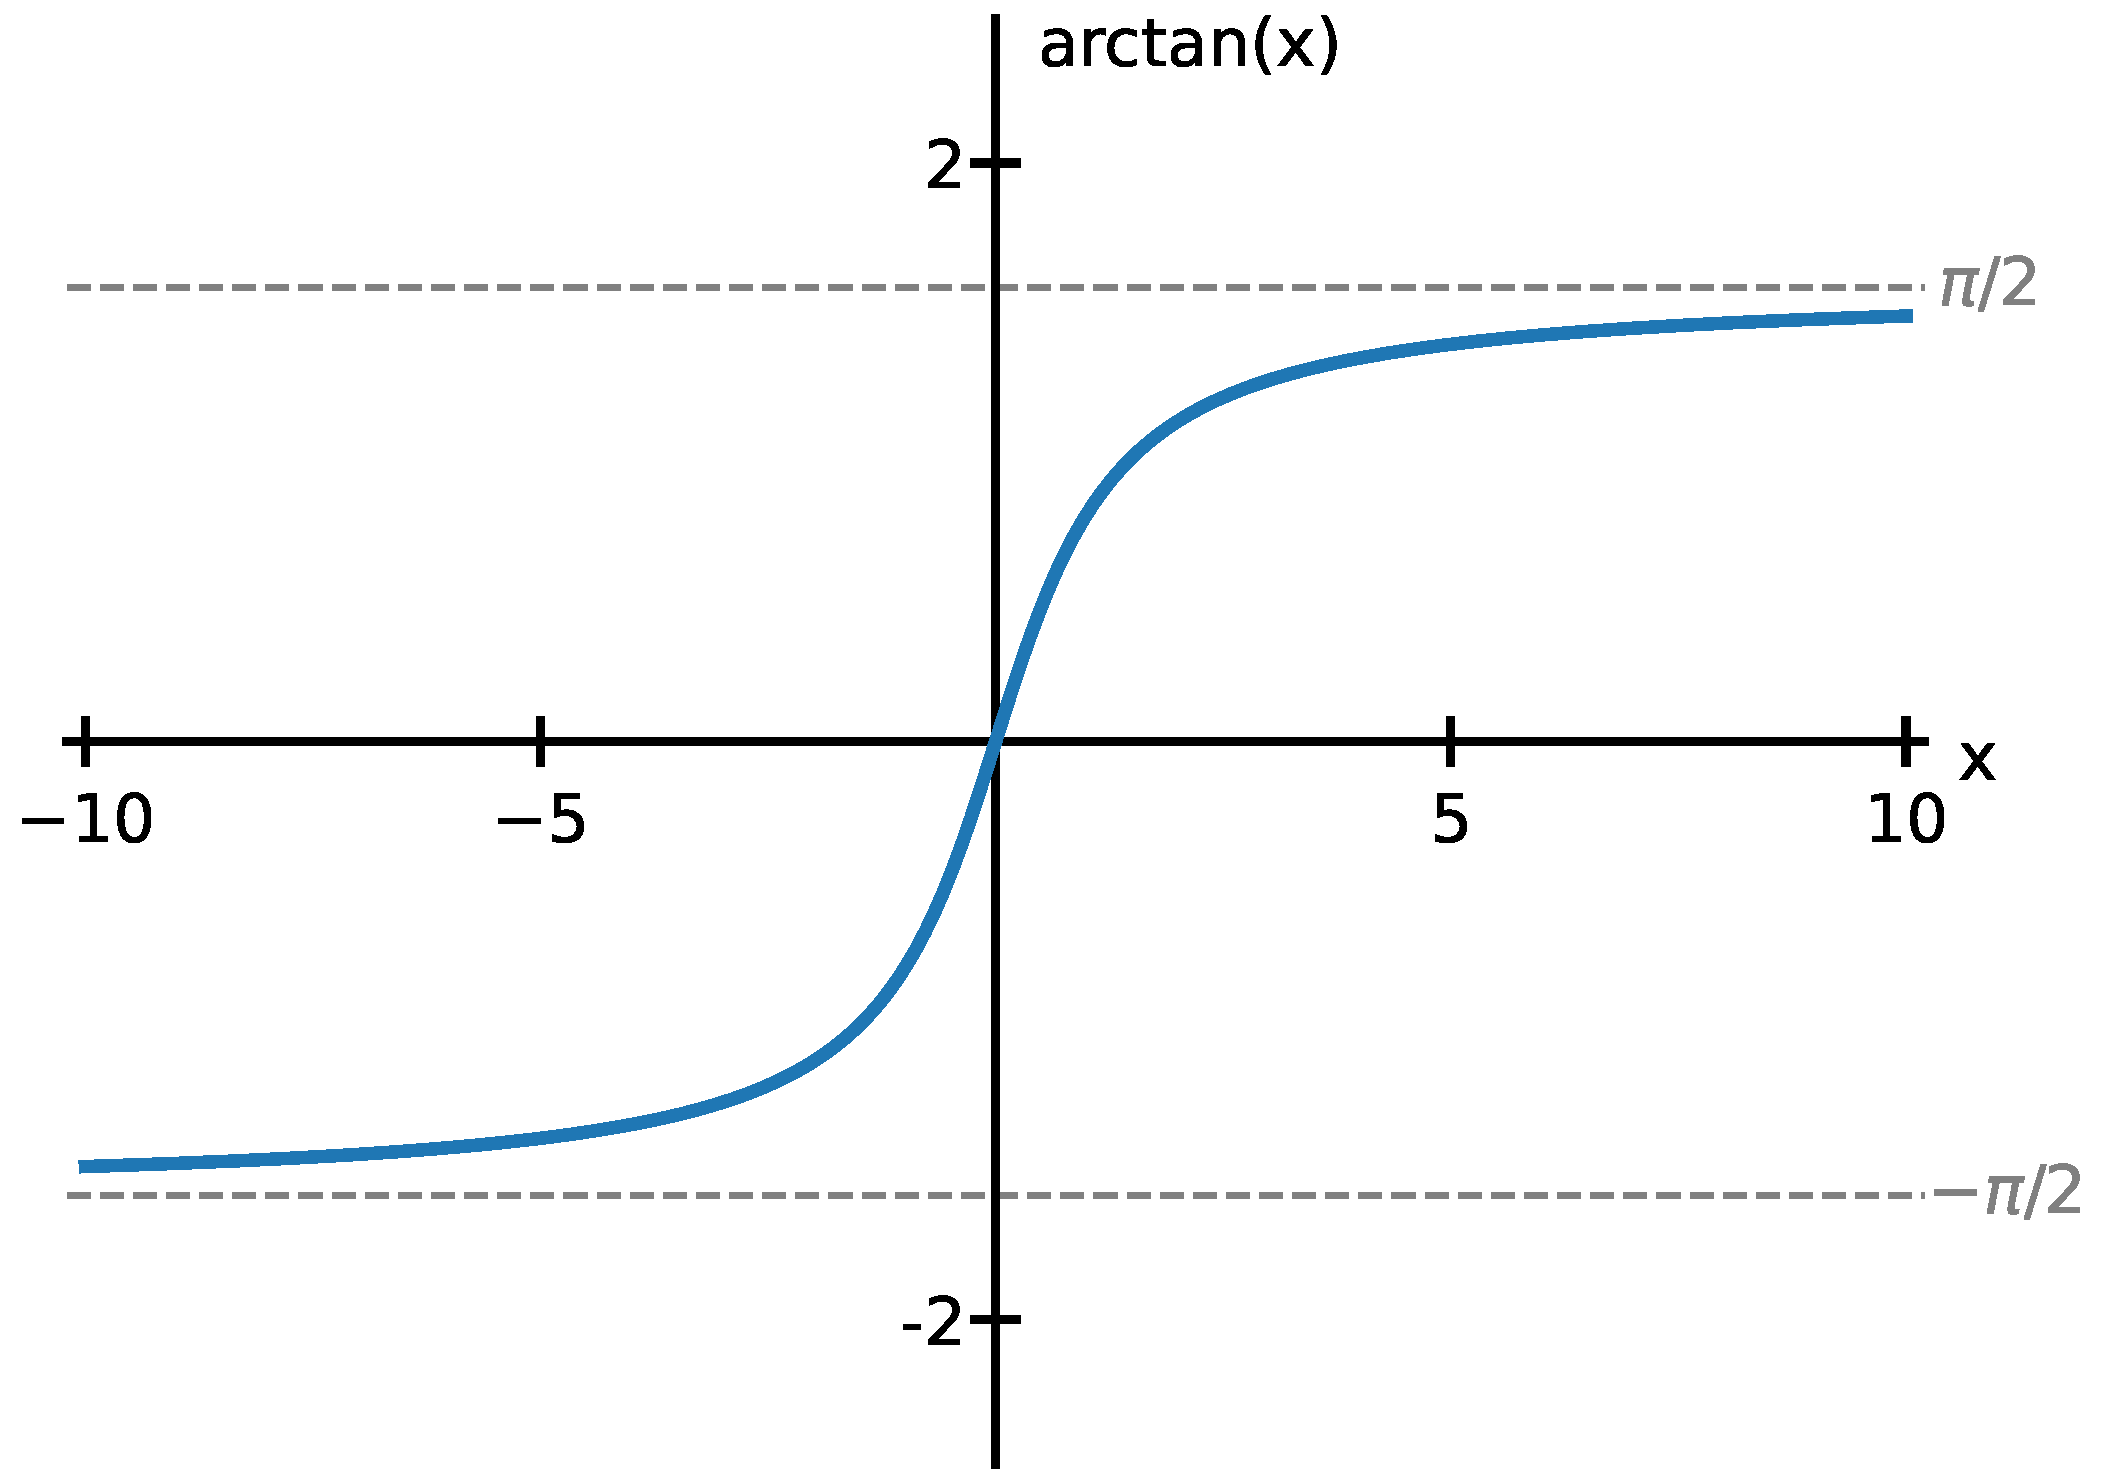
\includegraphics[width=\linewidth, trim={0, 0, 0, 0},clip]{icml2024/figures/arctangent/arctan_plot_wide.pdf}
        \caption{Arctangent function}
        \label{fig:appendix_arctan_function}
    \end{minipage}
    \hfill %
    \begin{minipage}[b]{0.48\linewidth} %
        \centering
        \begingroup
        \renewcommand{\arraystretch}{1.7}
        \begin{tabular}{|c|c|c|}
        \hline
         $b$ & $a$, if $m \ll \sqrt{v}$ & $a$, if $m \sim \sqrt{v}$ \\ \hline
         1 & 1 & $1/\arctan(1) = 1.27$ \\ \hline
         2 & 2 & $1/\arctan(\frac{1}{2}) = 2.16$ \\ \hline
         4 & 4 & $1/\arctan(\frac{1}{4}) = 4.08$ \\ \hline
         8 & 8 & $1/\arctan(\frac{1}{8}) = 8.04$ \\ \hline
         16 & 16 & $1/\arctan(\frac{1}{16}) = 16.02$ \\ \hline
         32 & 32 & $1/\arctan(\frac{1}{32}) = 32.01$ \\ \hline 
        \end{tabular}
        \vspace{12pt}
        \captionof{table}{Constants $a$ and $b$ for scaling arctangent.}
        \label{tab:arctan_constants}
        \endgroup
    \end{minipage}
    }
\end{figure*}


Regarding the constant values $a$ and $b$, using a value of $b > 1$ rescales the argument to be closer to zero which extends the region where arctangent acts as a small-angle approximation. For a given $b$, the choice of $a$ controls the approximation when the argument is far from zero. We note, however, that changing the value of $a$ simply rescales the effective learning rate and would be absorbed into a sweep of the base learning rate.

Depending on the relationship between $m$ and $v$, we derive different values of $a$ that would preserve the effective learning rate for Adam for a particular value of $b$. Recall that $m$ and $v$ are the first- and second-order moment estimates of the gradient, so when the moving average is up-to-date then $\norm{m} \leq \norm{\sqrt{v}}$ and the arctangent argument will be in the range $[-1/b, 1/b]$. If $m << \sqrt{v}$, to give an accurate small-angle approximation, we want $a=b$ so that the first term in the Taylor series $a \cdot \arctan(x, b\cdot y) = \frac{a}{by} x + \ldots$ matches the usual division operator that is linear in $x$ with coefficient $1/y$. If $m \sim \sqrt{v}$, to give an accurate approximation when $m / \sqrt{v}$ approaches $\pm 1$, we want $a = \frac{1}{arctan(1/b)}$ so that $a \cdot \arctan(m, b \cdot \sqrt{v}) = a \cdot arctan(1/b) = 1$. For $b=1$, this corresponds to $a = 4 / \pi \approx 1.27$. It is therefore possible that our choice of $a=1$ when $b=1$ may induce a change of up to this $\approx 1.27$ factor in the effective learning rate, but this change would be absorbed into our learning rate sweeps. We note in \cref{tab:arctan_constants} that as $b$ becomes larger, the values from $a$ converge between these two regimes.













\newcommand{\figwidth}{0.2\paperwidth}
\newcommand{\figvspace}{\vspace{0.5cm}}
\newcommand{\appsinglefigure}[1]{\includegraphics[width=\figwidth, trim={0, 0, 0, 0},clip]{#1}}


\newcommand{\appfigure}[2]{
    \centerline{
        \appsinglefigure{icml2024/appendix_figures/lr_sweep/#1+stp+50k_steps#2.pdf}
        \appsinglefigure{icml2024/appendix_figures/power_law/#1+stp+50k_steps#2.pdf}
        \appsinglefigure{icml2024/appendix_figures/lr_sweep/#1+stp+compute_opt#2.pdf}
        \appsinglefigure{icml2024/appendix_figures/power_law/#1+stp+compute_opt#2.pdf}
    }
    \centerline{
        \appsinglefigure{icml2024/appendix_figures/lr_sweep/#1+ntk+50k_steps#2.pdf}
        \appsinglefigure{icml2024/appendix_figures/power_law/#1+ntk+50k_steps#2.pdf}
        \appsinglefigure{icml2024/appendix_figures/lr_sweep/#1+ntk+compute_opt#2.pdf}
        \appsinglefigure{icml2024/appendix_figures/power_law/#1+ntk+compute_opt#2.pdf}
    }
    \centerline{
        \appsinglefigure{icml2024/appendix_figures/lr_sweep/#1+mup_table_9+50k_steps#2.pdf}
        \appsinglefigure{icml2024/appendix_figures/power_law/#1+mup_table_9+50k_steps#2.pdf}
        \appsinglefigure{icml2024/appendix_figures/lr_sweep/#1+mup_table_9+compute_opt#2.pdf}
        \appsinglefigure{icml2024/appendix_figures/power_law/#1+mup_table_9+compute_opt#2.pdf}
    }
    \centerline{
        \appsinglefigure{icml2024/appendix_figures/lr_sweep/#1+mfp+50k_steps#2.pdf}
        \appsinglefigure{icml2024/appendix_figures/power_law/#1+mfp+50k_steps#2.pdf}
        \appsinglefigure{icml2024/appendix_figures/lr_sweep/#1+mfp+compute_opt#2.pdf}
        \appsinglefigure{icml2024/appendix_figures/power_law/#1+mfp+compute_opt#2.pdf}
    }
}

\clearpage
\begin{figure*}[ht]
\subsection{Additional Alignment Experiments}
\label{app:alignment_expts}
\figvspace
\figvspace
    \begin{center}
        \textbf{SGD+Momentum Alignment Experiments}\\
        \figvspace
        
        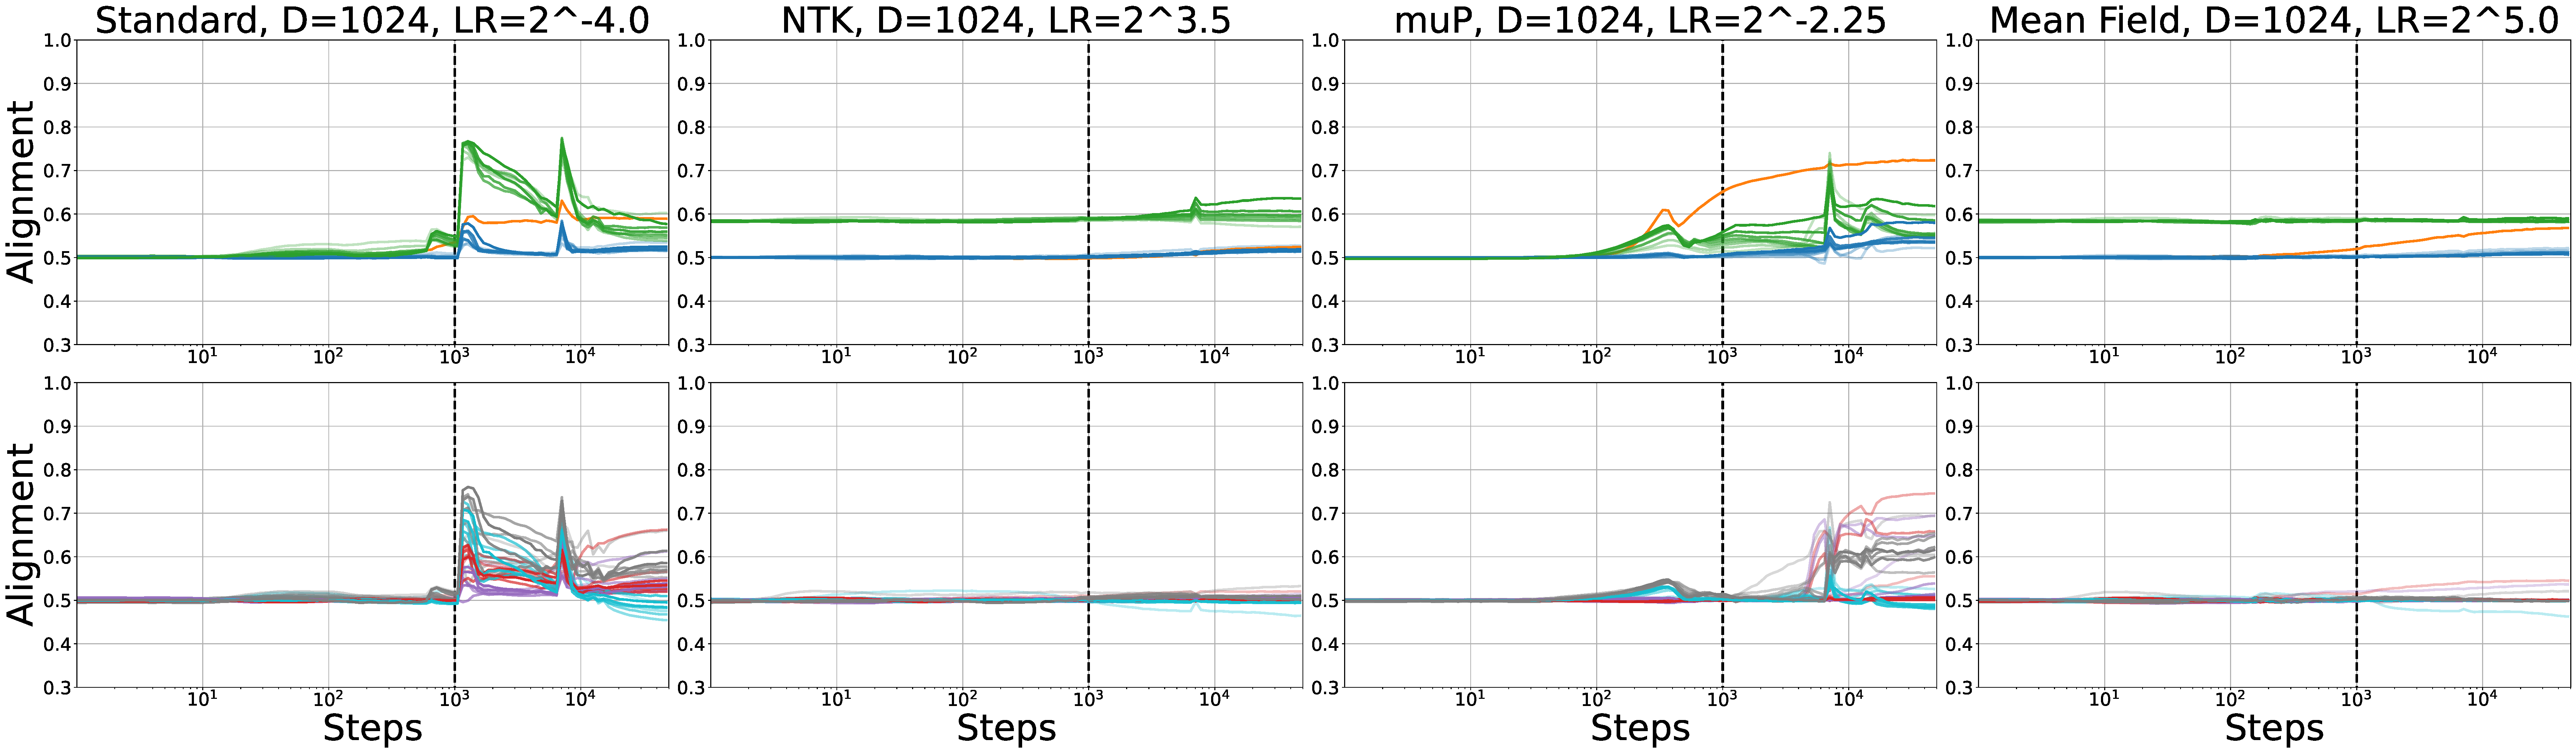
\includegraphics[width=\linewidth, trim={0, 0, 0, 0},clip]{icml2024/figures/alignment/appendix/sgdw_v2+momentum_1024.pdf}
       
        \figvspace
        \figvspace
       
        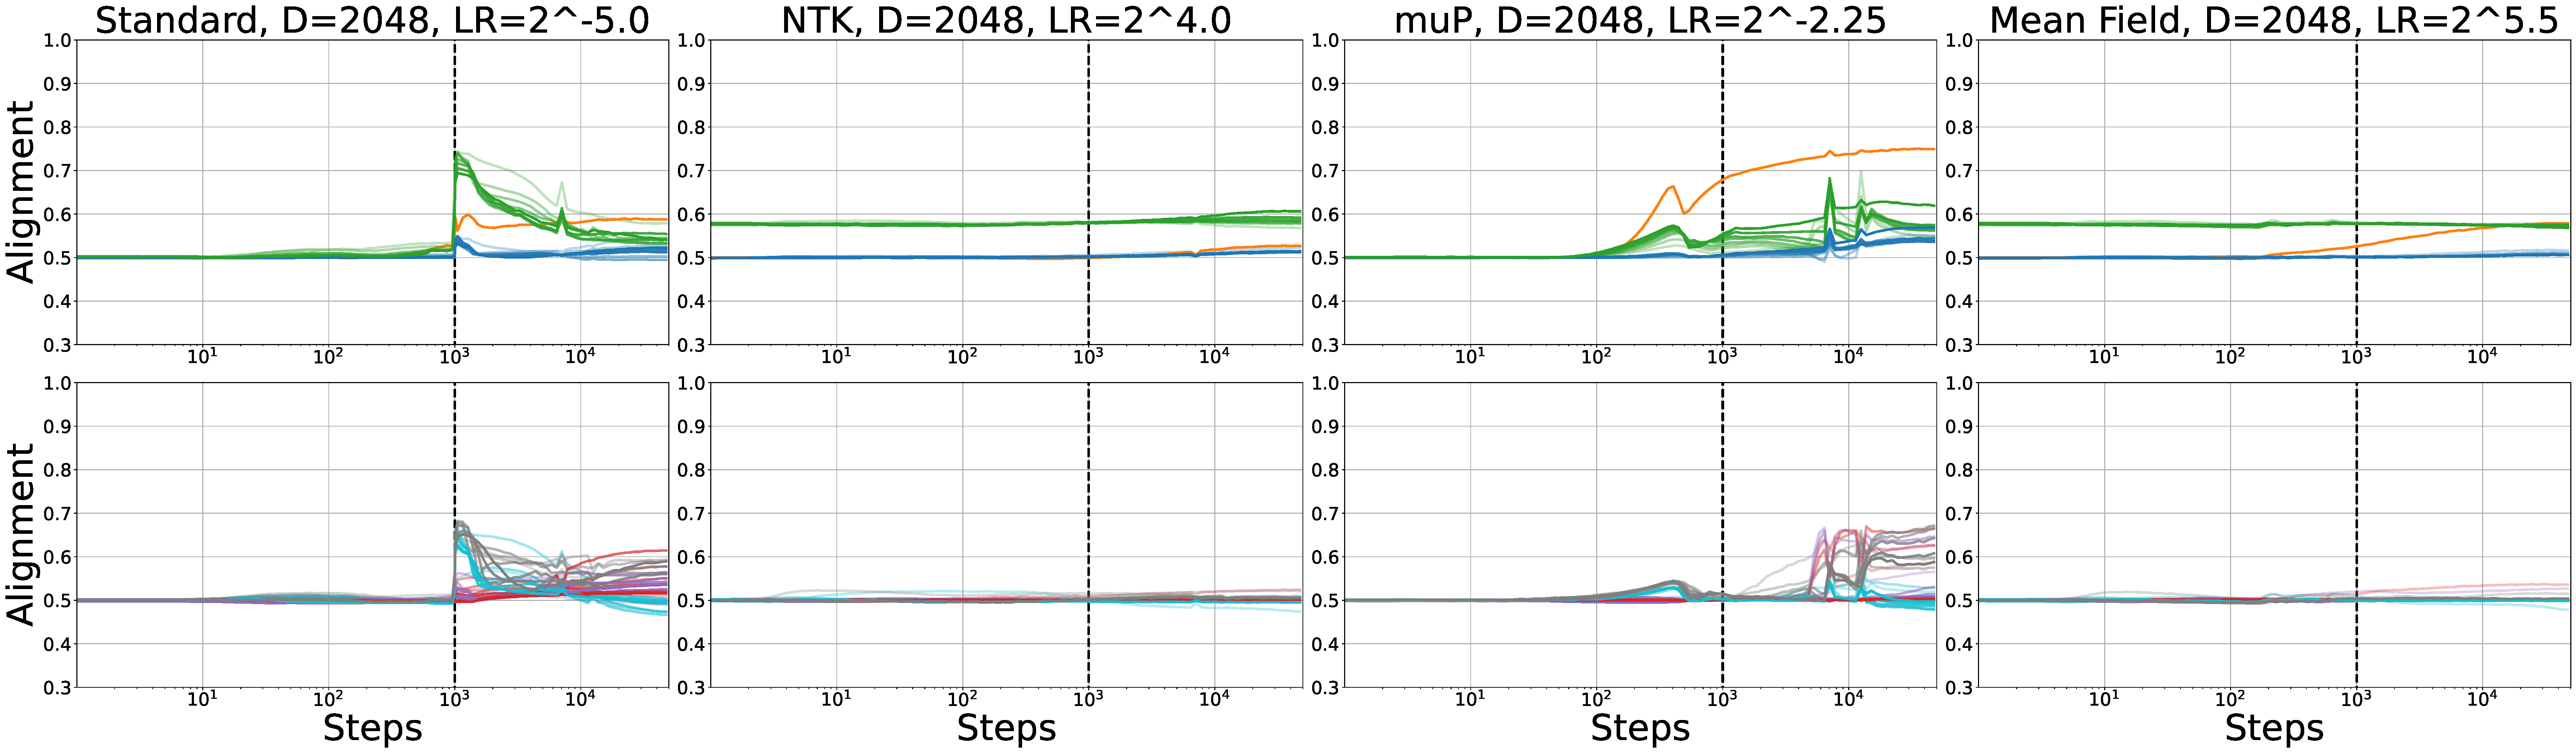
\includegraphics[width=\linewidth, trim={0, 0, 0, 0},clip]{icml2024/figures/alignment/appendix/sgdw_v2+momentum_2048.pdf}
       
        \figvspace
        \figvspace
       
        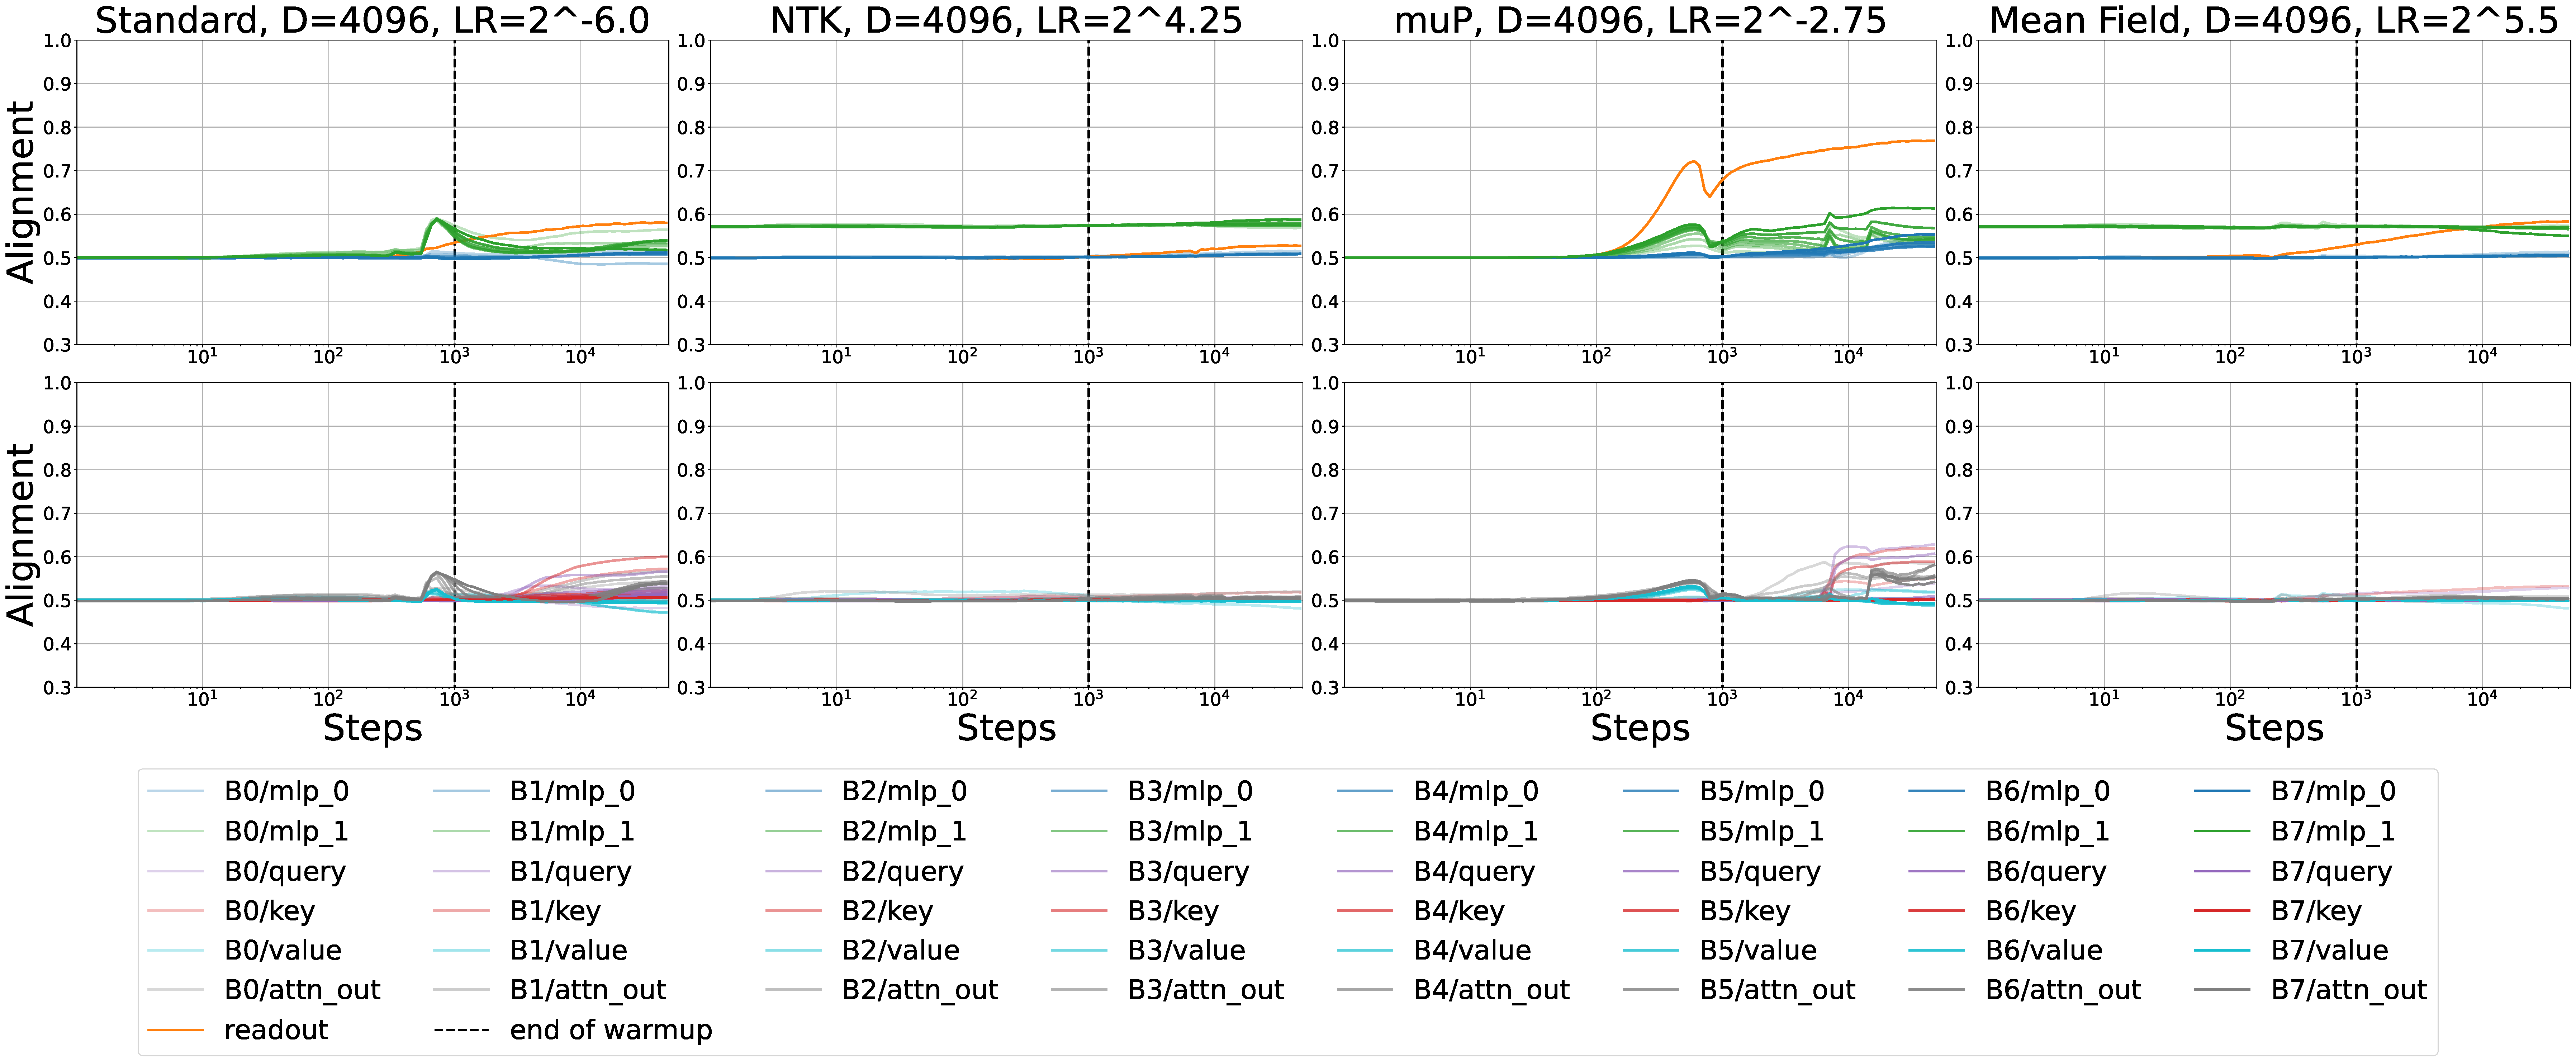
\includegraphics[width=\linewidth, trim={0, 0, 0, 0},clip]{icml2024/figures/alignment/appendix/sgdw_v2+momentum_4096_legend.pdf}
        \caption{The log alignment ratio measured in all dense layers across training steps for SGD using a global learning rate at approximately the optimal learning rate for each setting. Top = $167M$ parameter model $(D=1024)$, middle = $535M$ parameter model $(D=2048)$, bottom = $1.9B$ parameter model $(D=4096)$. Note the log scale on the x-axis.}
        \figvspace
        \label{fig:appendix_alignment_sgd}
    \end{center}
\end{figure*}
\clearpage

\begin{figure*}[ht]
    \begin{center}
        \textbf{Adam Alignment Experiments}\\
        \figvspace
        
        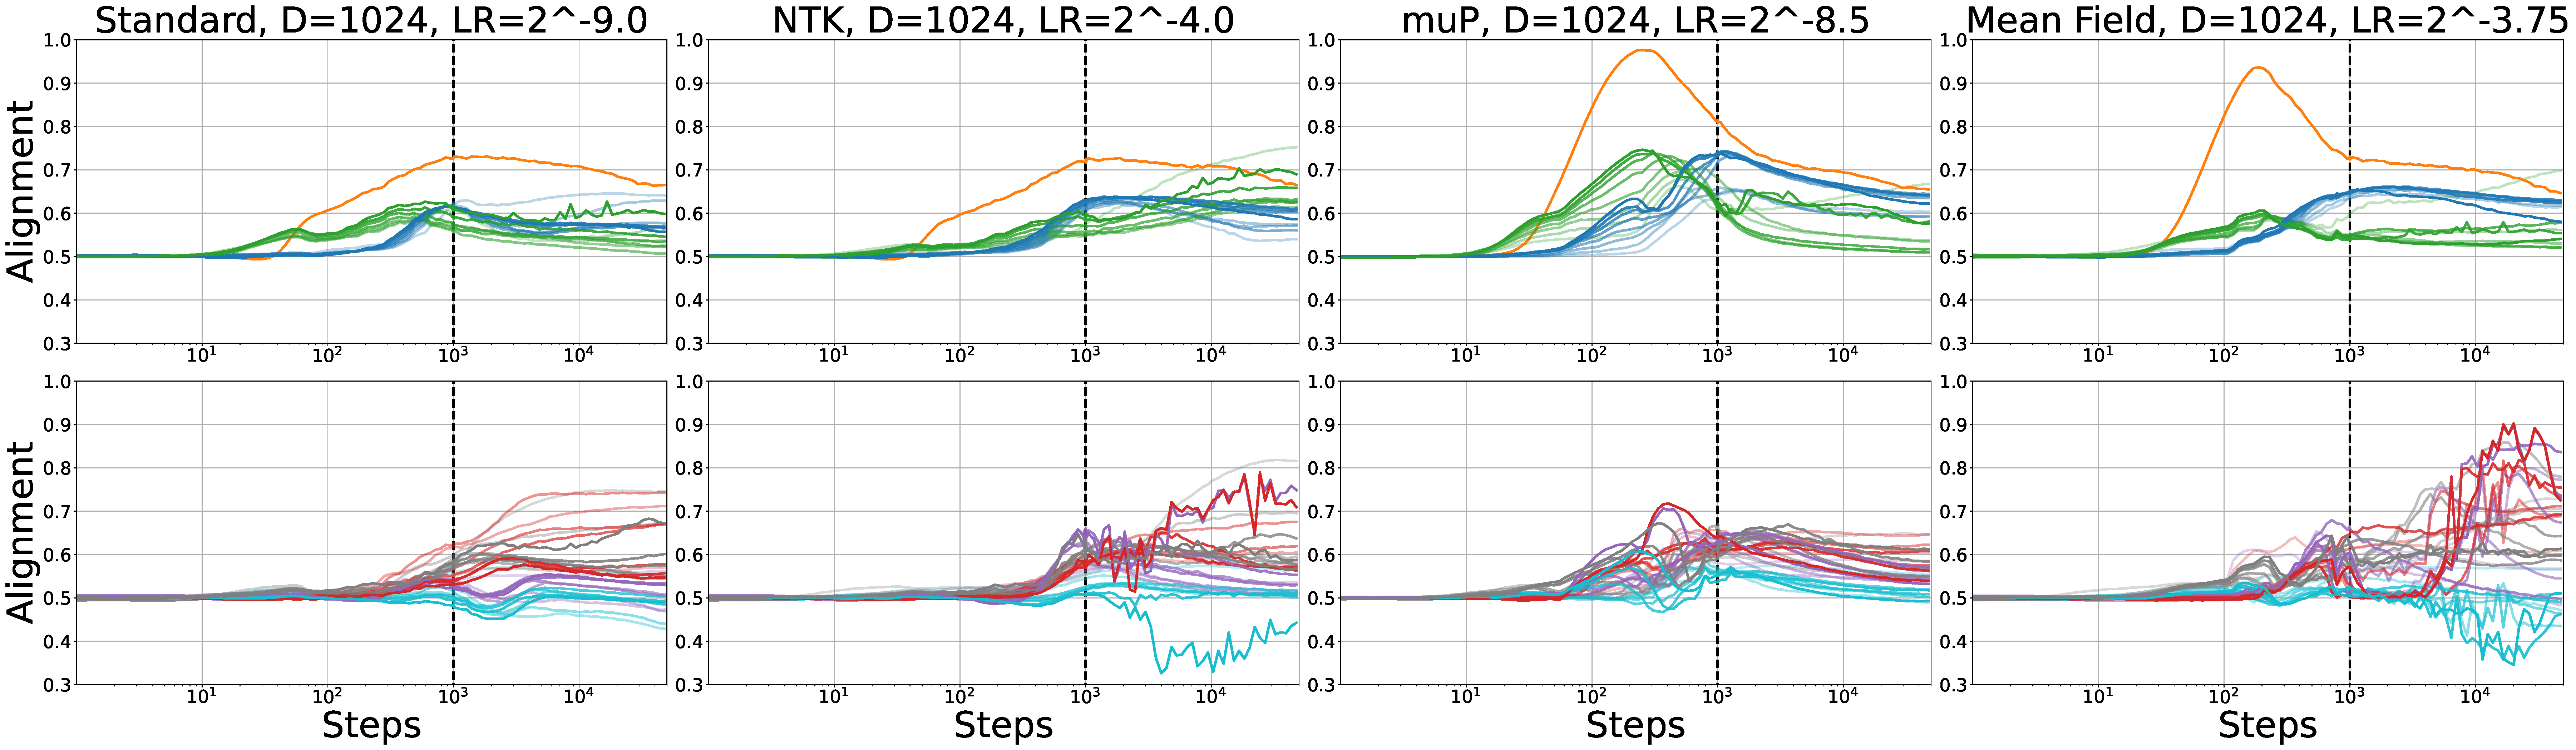
\includegraphics[width=\linewidth, trim={0, 0, 0, 0},clip]{icml2024/figures/alignment/appendix/adamw_1024.pdf}
       
        \figvspace
        \figvspace
       
        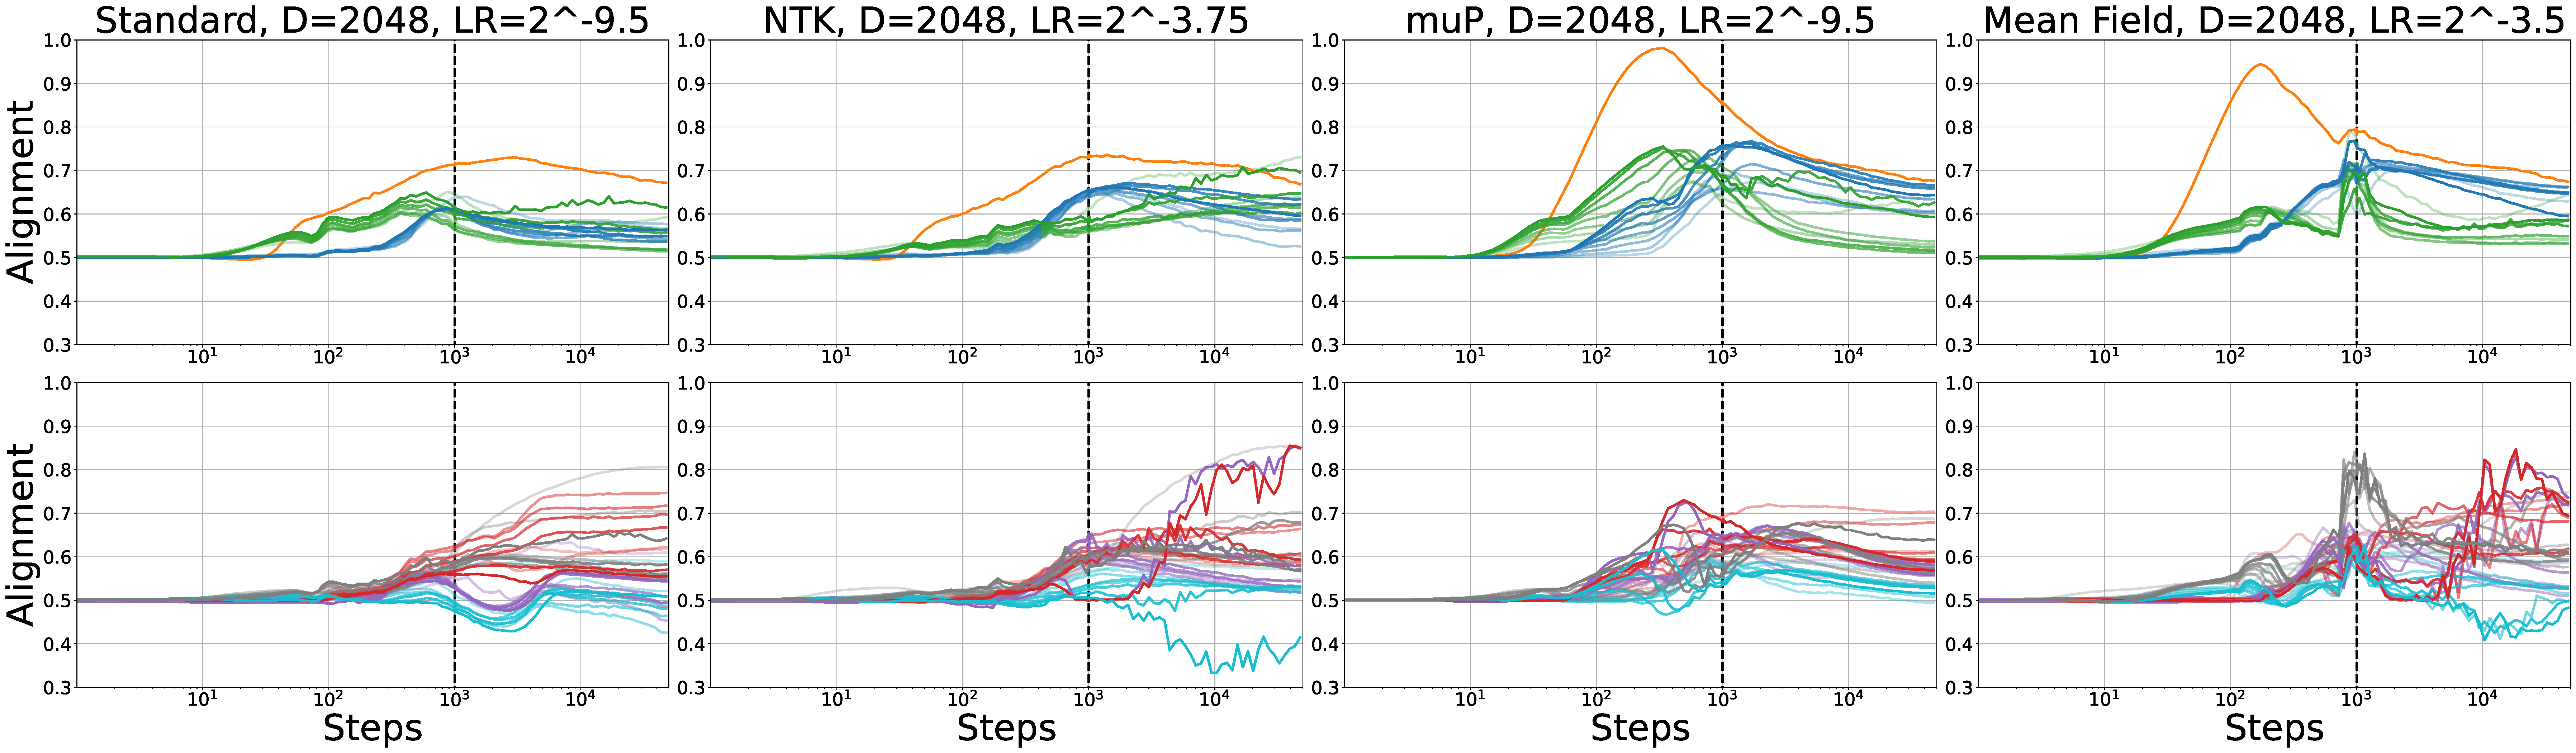
\includegraphics[width=\linewidth, trim={0, 0, 0, 0},clip]{icml2024/figures/alignment/appendix/adamw_2048.pdf}
       
        \figvspace
        \figvspace
       
        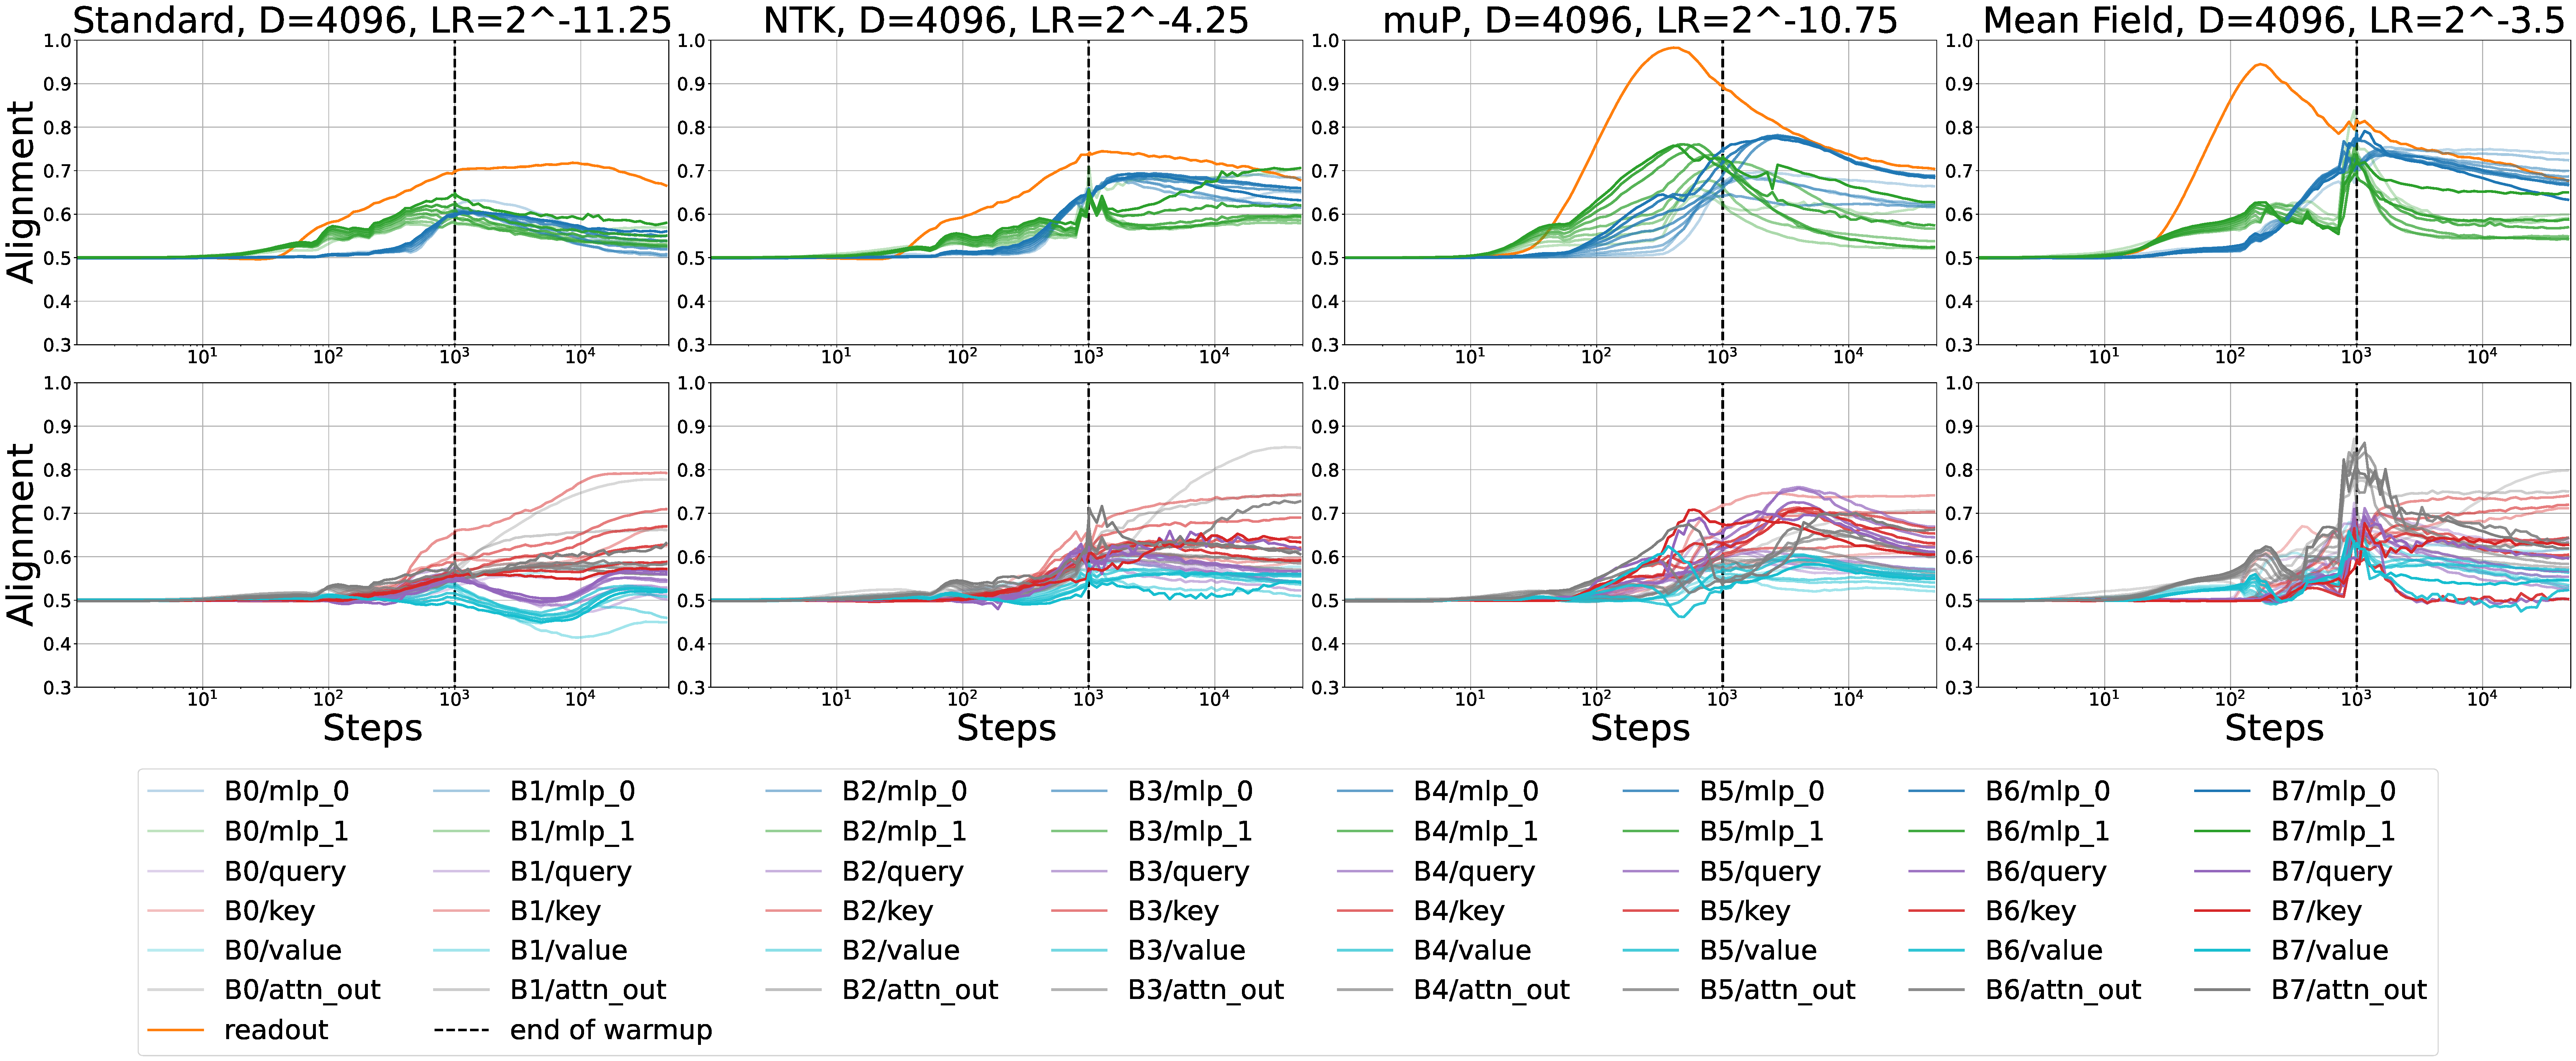
\includegraphics[width=\linewidth, trim={0, 0, 0, 0},clip]{icml2024/figures/alignment/appendix/adamw_4096_legend.pdf}
        \caption{The log alignment ratio measured in all dense layers across training steps for Adam using a global learning rate at approximately the optimal learning rate for each setting. Top = $167M$ parameter model $(D=1024)$, middle = $535M$ parameter model $(D=2048)$, bottom = $1.9B$ parameter model $(D=4096)$. Note the log scale on the x-axis.}
        \label{fig:appendix_alignment_adam}
    \end{center}
\end{figure*}
\newpage


\begin{figure*}[ht]
    \begin{center}
        \textbf{Adafactor Alignment Experiments}\\
        \figvspace
        
        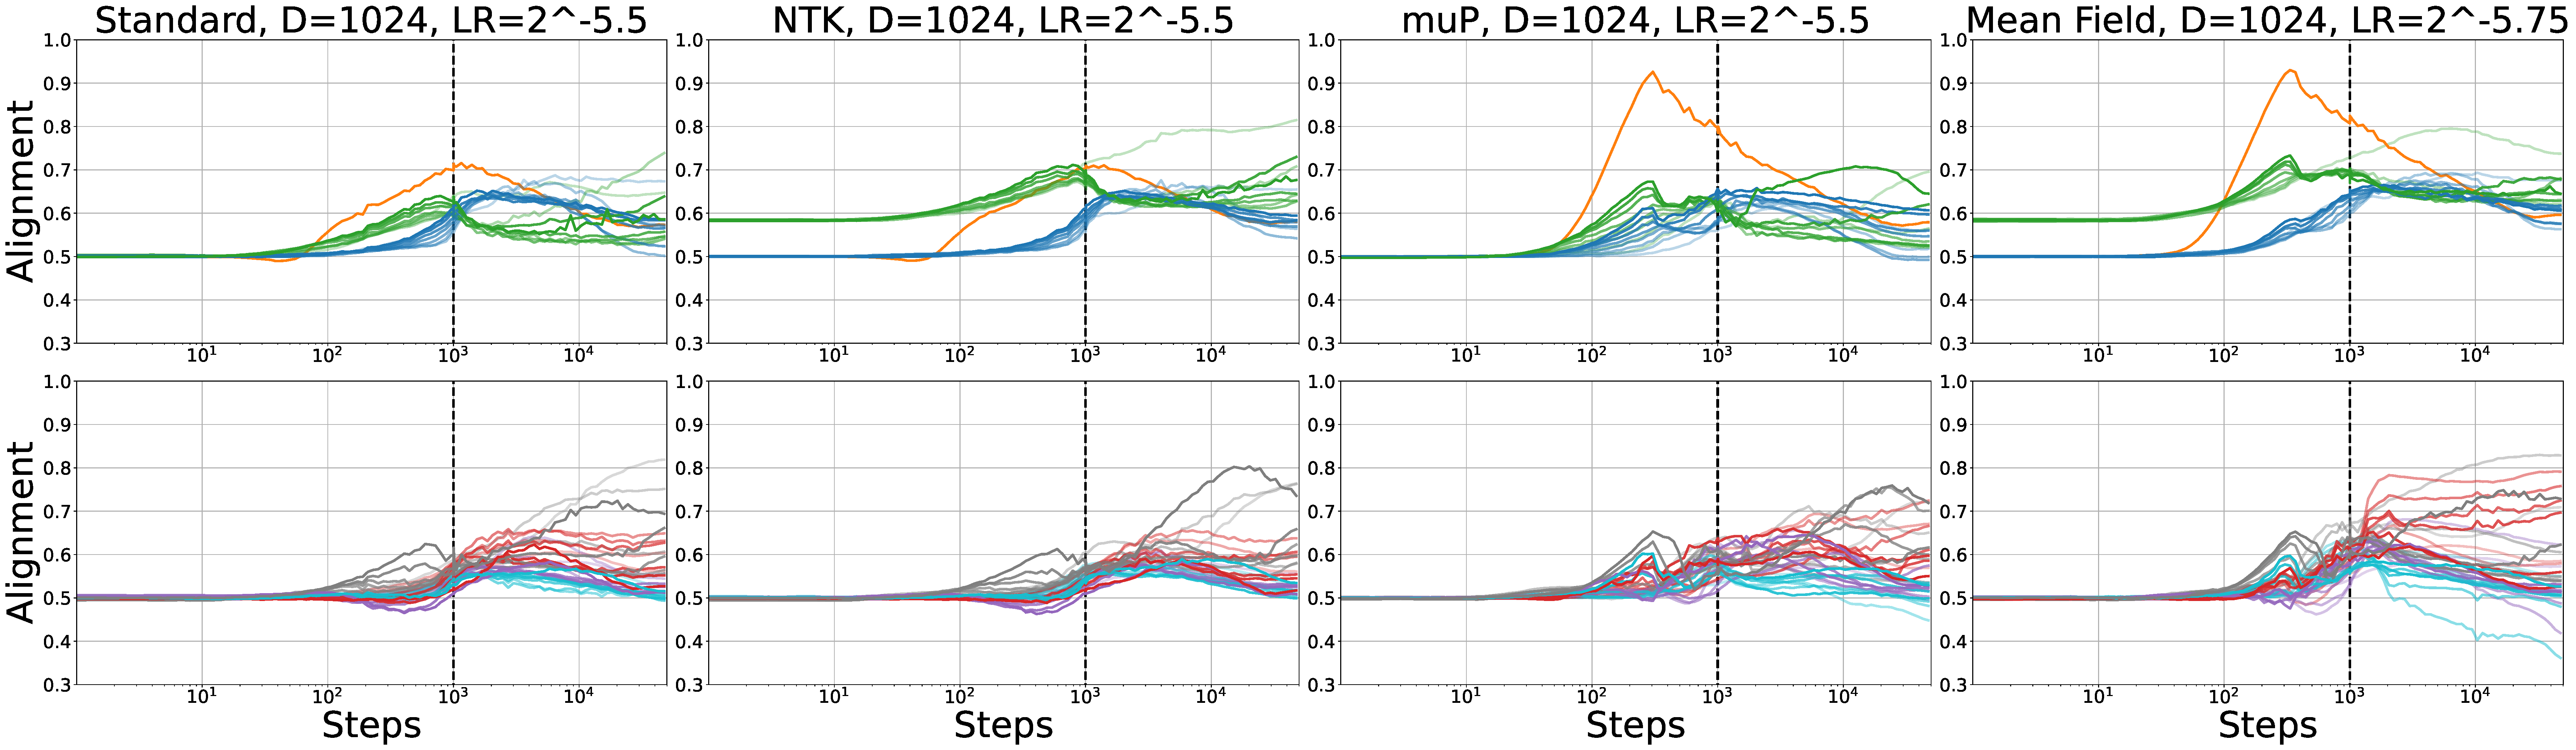
\includegraphics[width=\linewidth, trim={0, 0, 0, 0},clip]{icml2024/figures/alignment/appendix/adafactor_ps_on_1024.pdf}
       
        \figvspace
        \figvspace
       
        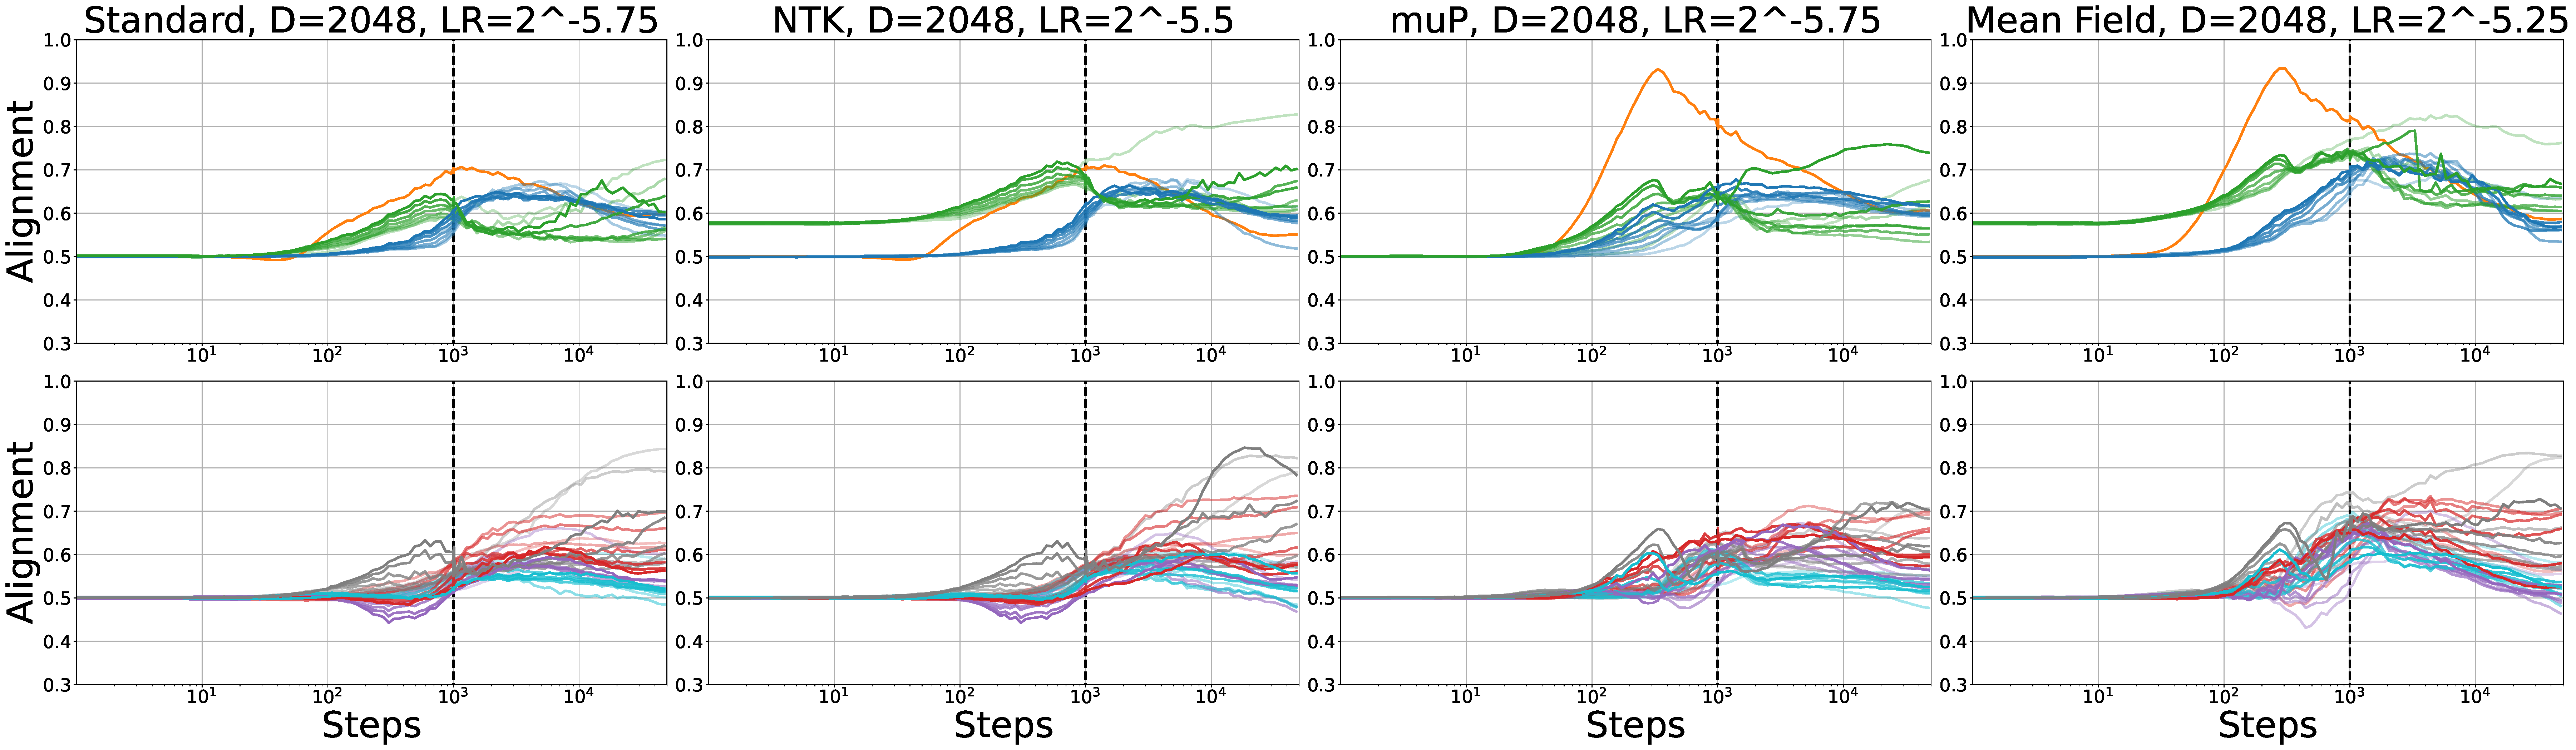
\includegraphics[width=\linewidth, trim={0, 0, 0, 0},clip]{icml2024/figures/alignment/appendix/adafactor_ps_on_2048.pdf}
       
        \figvspace
        \figvspace
       
        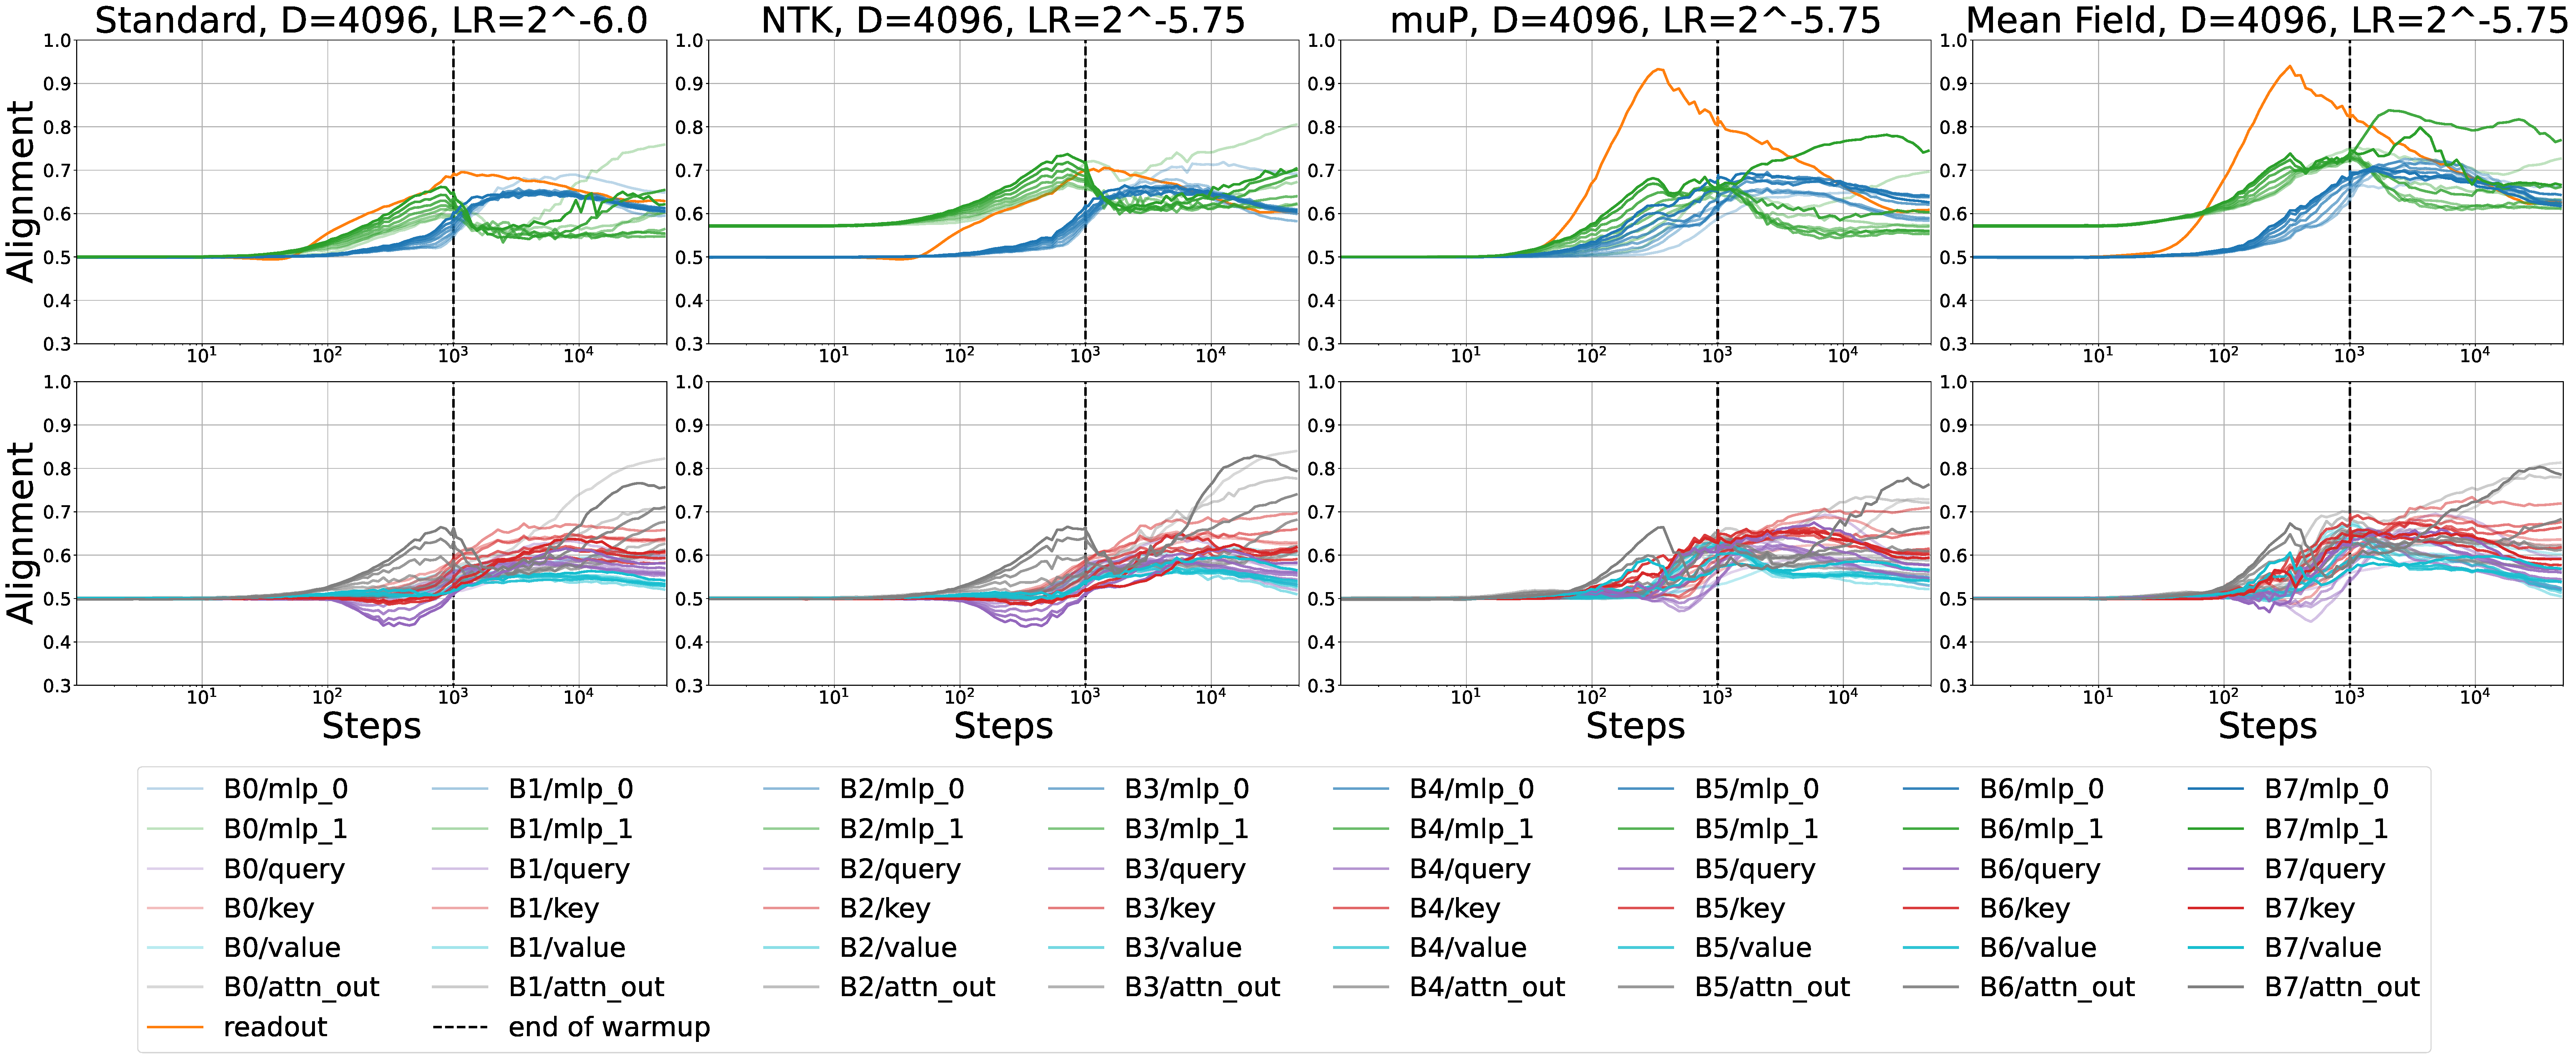
\includegraphics[width=\linewidth, trim={0, 0, 0, 0},clip]{icml2024/figures/alignment/appendix/adafactor_ps_on_4096_legend.pdf}
        \caption{The log alignment ratio measured in all dense layers across training steps for Adafactor using a global learning rate at approximately the optimal learning rate for each setting. Top = $167M$ parameter model $(D=1024)$, middle = $535M$ parameter model $(D=2048)$, bottom = $1.9B$ parameter model $(D=4096)$. Note the log scale on the x-axis.}
        \label{fig:appendix_alignment_adafactor}
    \end{center}
\end{figure*}
\clearpage

\subsection{Additional Per-Layer Learning Rate Experiment Results}
\label{sec:app_per_layer_lr_results}
This section includes additional results for the per-layer learning rate experiments in \cref{sec:results_per_layer}. In \cref{fig:app_hparam_transfer_align_comparison}, we show the difference in the scale-dependence of the optimal learning rate for the full alignment vs no alignment settings for Adam. In \cref{tab:appendix_table} we report the eval losses for the six largest model sizes in all settings including per-layer epsilon settings. In \cref{fig:app_scaling_optimal_constants}, we show eval loss vs model size scaling curves for all optimizers for all settings that use optimal per-layer learning rate constant multipliers. In \cref{fig:app_scaling_ablation}, we include eval loss vs model size scaling curves for an ablation of global vs per-layer learning rates and default vs optimal constants. Learning rate sweeps for all settings are included in \sref{sec:app_lr_sweeps_sgd}, \sref{sec:app_lr_sweeps_adam} and \sref{sec:app_lr_sweeps_adam_ps}.


\vfill
\begin{figure}[h]
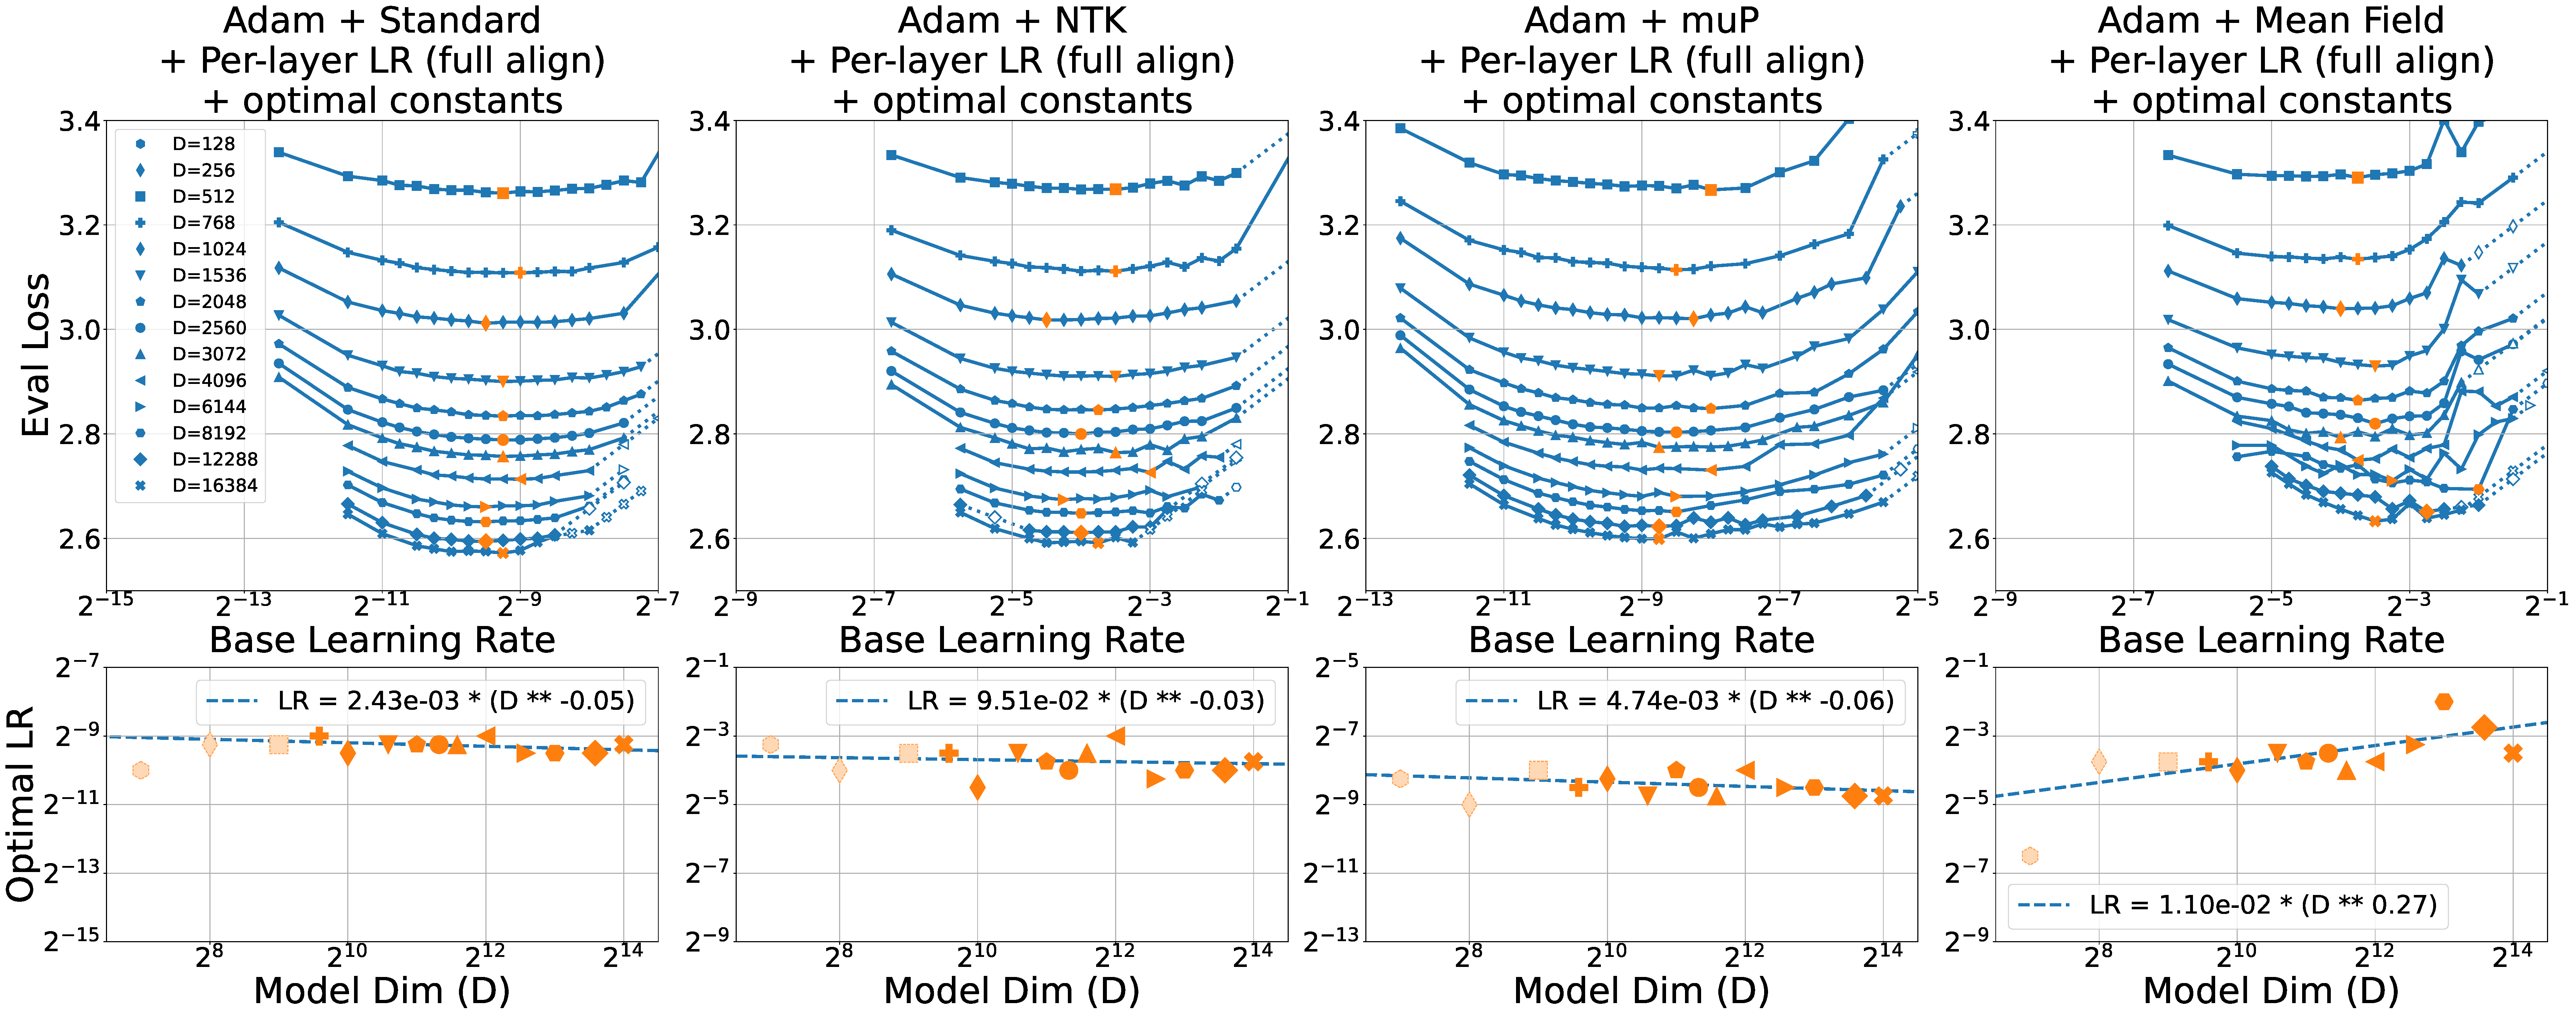
\includegraphics[width=\linewidth]{icml2024/figures/lr_sweeps/appendix/adam/adam+50k_steps_per_module_lr_optimal_constants.pdf}

\figvspace

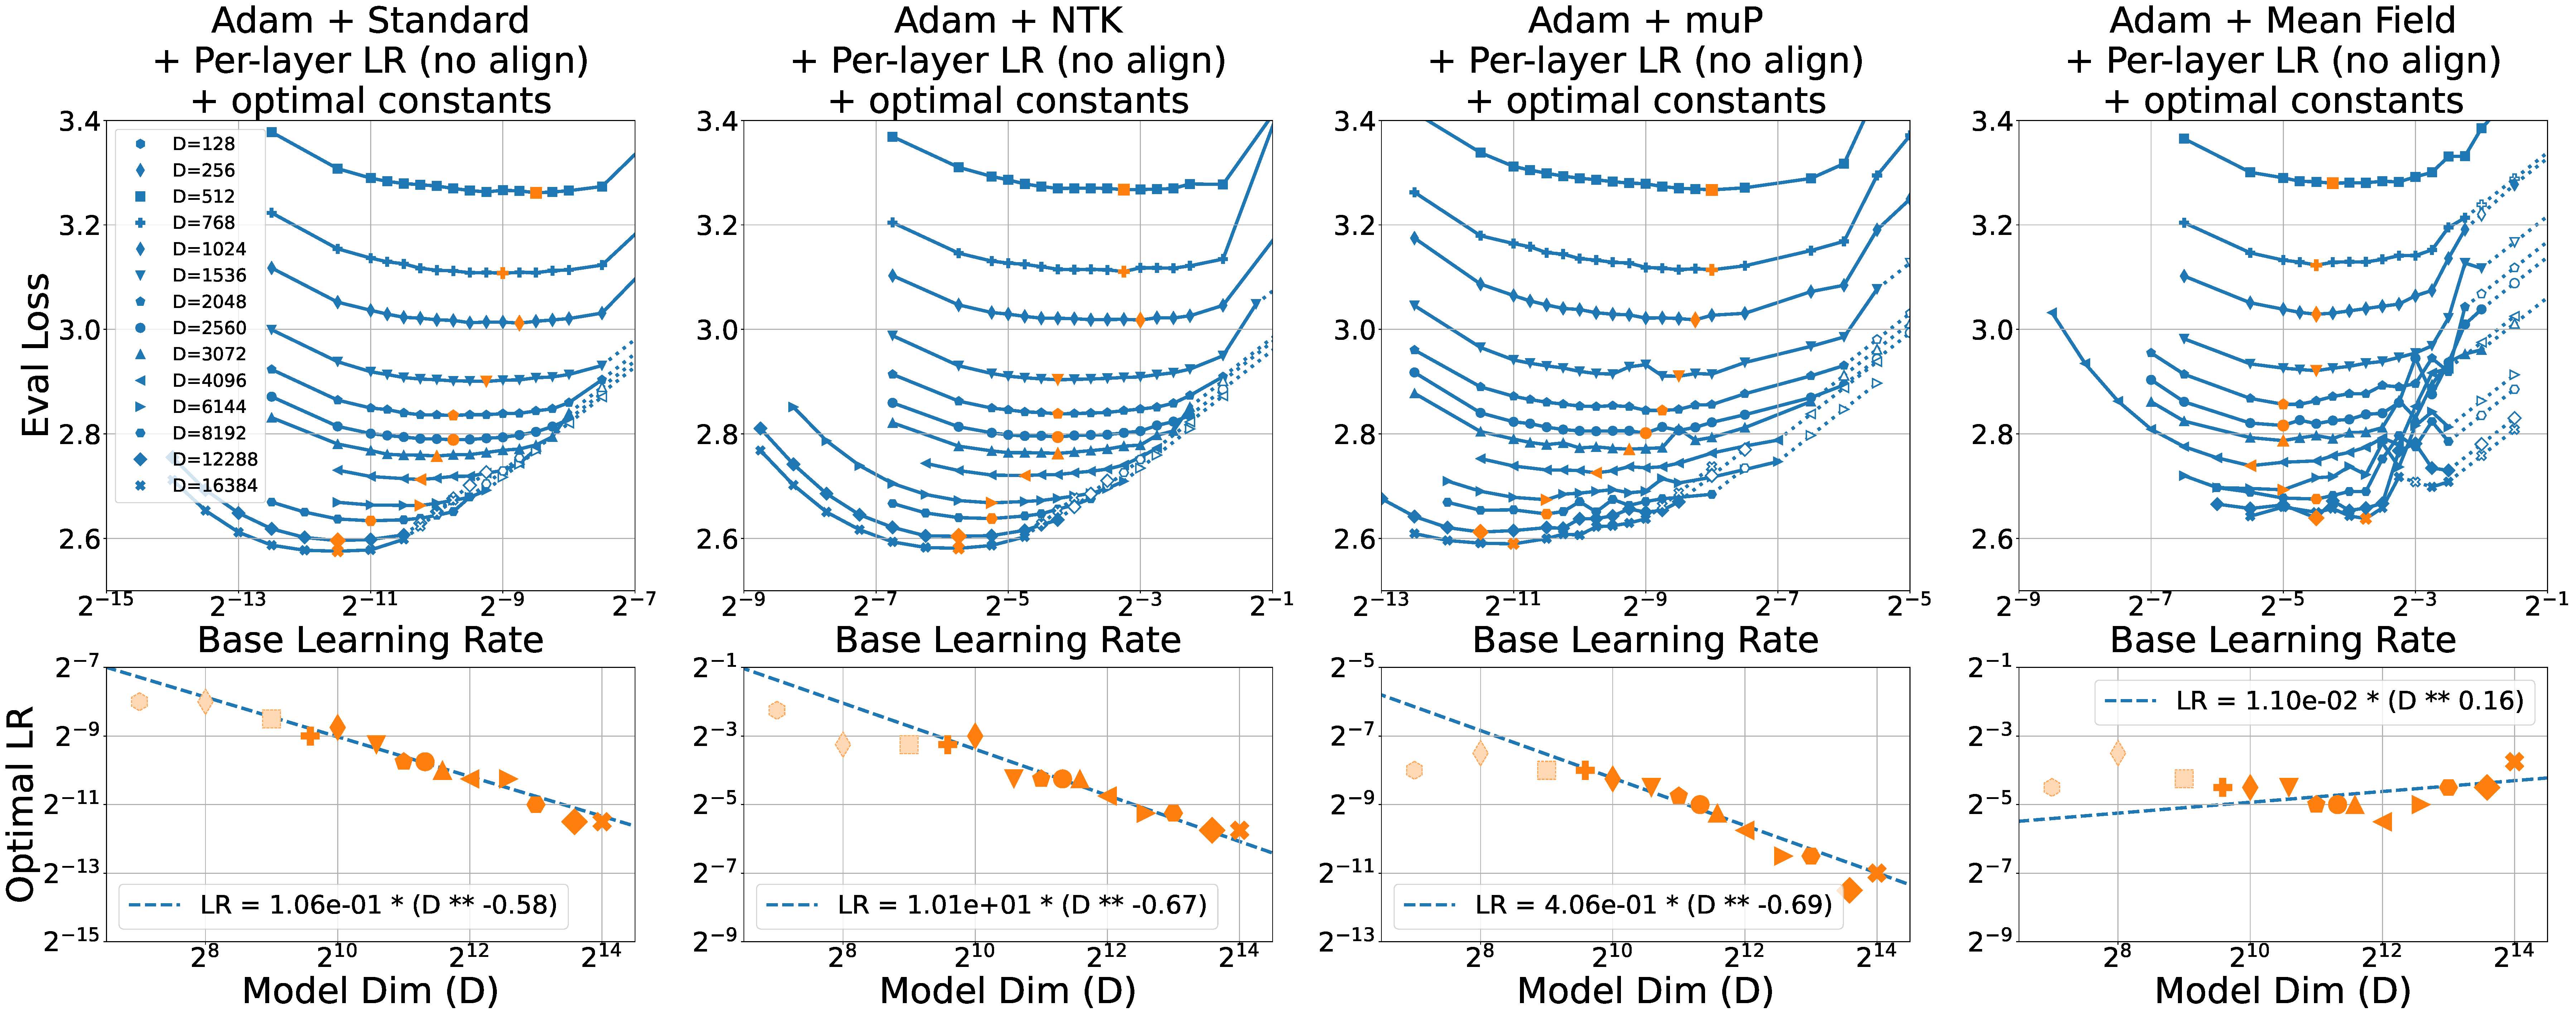
\includegraphics[width=\linewidth]{icml2024/figures/lr_sweeps/appendix/adam/adam+50k_steps_per_module_lr_optimal_constants_no_align.pdf}
\caption{\textbf{Despite slight improvements in the eval loss under no alignment assumptions for NTK, muP and MFP, the full alignment experiments show better scale-invariance of the optimal learning rate.} Learning rate sweeps and power laws fit to optimal learning rate vs model dim. Top = Adam + per-layer learning rates assuming full alignment + optimal constants. Bottom = Adam + per-layer learning rates assuming no alignment + optimal constants. Number of training steps = $50{,}000$.}
\label{fig:app_hparam_transfer_align_comparison}
\end{figure}
\vfill
\clearpage

\begingroup
\renewcommand{\arraystretch}{1}
\begin{table*}[h!]
\centering
\caption{\textbf{Best eval losses for six largest model sizes.} For each optimizer $\times$ parameterization $\times$ model size $\times$ setting, we sweep the base LR and report the best eval loss. For per-layer epsilon experiments (rightmost two columns), we use base epsilon = 1e-12.}
\label{tab:appendix_table}
\adjustbox{scale=0.6}{
\begin{tabularx}{1.65\textwidth}{XXX | XXXXXXX}
\toprule[1.5\heavyrulewidth]
& & & Global LR \newline+ default & Global LR \newline+ optimal & Per-layer LR \newline+ full align \newline+ default & Per-layer LR \newline+ full align \newline+ optimal & Per-layer LR \newline+ no align \newline+ optimal & Per-layer LR \newline+ perf align \newline+ optimal \newline+ per-layer eps & Per-layer LR \newline+ no align \newline+ optimal \newline+ per-layer eps\\
\midrule[\heavyrulewidth]
\multirow{24}{*}{\Large SGD} & \multirow{6}{*}{\Large STP } & 1.1B & 3.464 & 3.256 & 3.810 & \textbf{3.122} & 3.252 &  &  \\ &  & 1.9B & 3.749 & \textbf{3.178} & 3.543 & 3.345 & 3.302 &  &  \\ &  & 4B & \textbf{3.220} & \textbf{3.220} & 3.628 & 3.264 & 3.294 &  &  \\ &  & 7B & 3.414 & 3.214 & 3.601 & 3.124 & \textbf{3.089} &  &  \\ &  & 15.3B & 3.172 & 3.074 & 3.386 & \textbf{3.037} & 3.377 &  &  \\ &  & 26.8B & 3.657 & \textbf{3.312} & 3.510 & 3.385 & 3.318 &  &  \\  \cmidrule{2-10}  & \multirow{6}{*}{\Large NTK } & 1.1B & 4.029 & \textbf{3.087} & 4.134 & 3.305 & 3.160 &  &  \\ &  & 1.9B & 4.029 & 3.385 & 4.029 & 3.374 & \textbf{3.325} &  &  \\ &  & 4B & 3.726 & 3.393 & 3.791 & \textbf{3.247} & 3.412 &  &  \\ &  & 7B & 3.794 & 3.134 & 3.704 & \textbf{3.076} & 3.087 &  &  \\ &  & 15.3B & 3.718 & 3.320 & 3.572 & \textbf{3.028} & 3.194 &  &  \\ &  & 26.8B & 3.732 & \textbf{3.210} & 3.627 & 3.313 & 3.324 &  &  \\  \cmidrule{2-10}  & \multirow{6}{*}{\Large muP } & 1.1B & 4.029 & 3.188 & 3.973 & 3.188 & \textbf{3.074} &  &  \\ &  & 1.9B & 3.883 & 3.759 & 3.883 & 3.759 & \textbf{3.050} &  &  \\ &  & 4B & 3.852 & 3.666 & 3.796 & 3.666 & \textbf{3.627} &  &  \\ &  & 7B & 3.464 & \textbf{3.098} & 3.532 & \textbf{3.098} & 3.828 &  &  \\ &  & 15.3B & 3.357 & 3.252 & 3.430 & 3.578 & \textbf{3.166} &  &  \\ &  & 26.8B & 4.224 & 3.810 & 4.184 & \textbf{3.809} & 4.222 &  &  \\  \cmidrule{2-10}  & \multirow{6}{*}{\Large MFP } & 1.1B & \textbf{3.805} & 4.010 & 4.255 & 4.082 & 4.095 &  &  \\ &  & 1.9B & 4.217 & 4.057 & 4.378 & 4.132 & \textbf{4.048} &  &  \\ &  & 4B & 4.131 & 3.795 & 3.939 & 3.946 & \textbf{3.782} &  &  \\ &  & 7B & 3.874 & 3.825 & 4.034 & 3.820 & \textbf{3.700} &  &  \\ &  & 15.3B & 3.968 & 3.910 & 4.131 & 3.945 & \textbf{3.742} &  &  \\ &  & 26.8B & 4.131 & 4.092 & 4.319 & 4.092 & \textbf{3.898} &  &  \\  \midrule[\heavyrulewidth] \multirow{24}{*}{\Large Adam} & \multirow{6}{*}{\Large STP } & 1.1B & 2.776 & 2.760 & 2.766 & \textbf{2.757} & 2.758 & \textbf{2.757} & 2.758 \\ &  & 1.9B & 2.734 & 2.715 & 2.717 & \textbf{2.713} & \textbf{2.713} & 2.714 & \textbf{2.713} \\ &  & 4B & 2.688 & 2.667 & 2.666 & \textbf{2.660} & 2.663 & 2.661 & 2.663 \\ &  & 7B & 2.665 & 2.641 & 2.636 & \textbf{2.632} & 2.634 & \textbf{2.632} & 2.633 \\ &  & 15.3B & 2.638 & 2.608 & 2.598 & 2.594 & 2.596 & \textbf{2.593} & 2.596 \\ &  & 26.8B & 2.625 & 2.590 & 2.576 & \textbf{2.572} & 2.575 & 2.573 & 2.576 \\  \cmidrule{2-10}  & \multirow{6}{*}{\Large NTK } & 1.1B & 2.782 & \textbf{2.761} & 2.789 & 2.764 & 2.763 & \textbf{2.761} & 2.763 \\ &  & 1.9B & 2.736 & 2.726 & 2.743 & 2.726 & 2.720 & \textbf{2.717} & 2.719 \\ &  & 4B & 2.672 & 2.674 & 2.695 & 2.674 & 2.668 & \textbf{2.665} & 2.666 \\ &  & 7B & 2.647 & 2.643 & 2.666 & 2.648 & 2.638 & \textbf{2.634} & 2.636 \\ &  & 15.3B & 2.605 & 2.605 & 2.634 & 2.611 & 2.604 & 2.600 & \textbf{2.597} \\ &  & 26.8B & 2.592 & 2.584 & 2.615 & 2.591 & 2.581 & \textbf{2.576} & 2.577 \\  \cmidrule{2-10}  & \multirow{6}{*}{\Large muP } & 1.1B & 2.822 & 2.773 & 2.802 & 2.774 & 2.771 & 2.773 & \textbf{2.770} \\ &  & 1.9B & 2.799 & 2.730 & 2.755 & 2.731 & \textbf{2.725} & 2.728 & 2.727 \\ &  & 4B & 2.756 & 2.682 & 2.714 & 2.680 & \textbf{2.674} & 2.680 & 2.679 \\ &  & 7B & 2.738 & 2.656 & 2.692 & 2.651 & 2.647 & 2.652 & \textbf{2.646} \\ &  & 15.3B & 2.729 & 2.628 & 2.664 & 2.623 & 2.612 & 2.623 & \textbf{2.611} \\ &  & 26.8B & 2.727 & 2.614 & 2.646 & 2.599 & \textbf{2.590} & 2.601 & \textbf{2.590} \\  \cmidrule{2-10}  & \multirow{6}{*}{\Large MFP } & 1.1B & 2.816 & 2.798 & 2.807 & 2.793 & 2.787 & \textbf{2.778} & 2.780 \\ &  & 1.9B & 2.770 & 2.756 & 2.756 & 2.750 & 2.739 & \textbf{2.736} & 2.738 \\ &  & 4B & 2.717 & 2.711 & 2.706 & 2.711 & 2.693 & 2.681 & \textbf{2.680} \\ &  & 7B & 2.699 & 2.693 & 2.686 & 2.694 & 2.675 & \textbf{2.645} & 2.649 \\ &  & 15.3B & 2.668 & 2.650 & 2.649 & 2.651 & 2.639 & 2.612 & \textbf{2.609} \\ &  & 26.8B & 2.638 & 2.649 & 2.630 & 2.633 & 2.638 & 2.590 & \textbf{2.583} \\  \midrule[\heavyrulewidth] \multirow{24}{*}{\makecell[l]{\Large Adam+\\\Large Param\\\Large Scaling}} & \multirow{6}{*}{\Large STP } & 1.1B & 2.778 & \textbf{2.760} & 2.784 & 2.779 & \textbf{2.760} & 2.815 & 2.765 \\ &  & 1.9B & 2.722 & 2.717 & 2.723 & 2.753 & 2.717 & 2.780 & \textbf{2.716} \\ &  & 4B & 2.668 & 2.668 & 2.677 & 2.730 & 2.668 & 2.737 & \textbf{2.667} \\ &  & 7B & 2.637 & 2.638 & 2.660 & 2.709 & 2.638 & 2.718 & \textbf{2.635} \\ &  & 15.3B & 2.600 & \textbf{2.599} & 2.630 & 2.687 & \textbf{2.599} & 2.691 & 2.601 \\ &  & 26.8B & 2.580 & 2.577 & 2.613 & 2.675 & 2.577 & 2.678 & \textbf{2.576} \\  \cmidrule{2-10}  & \multirow{6}{*}{\Large NTK } & 1.1B & 2.751 & 2.753 & 2.759 & 2.786 & 2.753 & 2.792 & \textbf{2.735} \\ &  & 1.9B & 2.699 & 2.698 & 2.722 & 2.752 & 2.698 & 2.760 & \textbf{2.690} \\ &  & 4B & 2.654 & 2.653 & 2.680 & 2.721 & 2.653 & 2.716 & \textbf{2.643} \\ &  & 7B & 2.624 & 2.626 & 2.658 & 2.703 & 2.626 & 2.696 & \textbf{2.613} \\ &  & 15.3B & 2.592 & 2.591 & 2.632 & 2.681 & 2.591 & 2.669 & \textbf{2.580} \\ &  & 26.8B & 2.570 & 2.566 & 2.623 & 2.667 & 2.566 & 2.654 & \textbf{2.554} \\  \cmidrule{2-10}  & \multirow{6}{*}{\Large muP } & 1.1B & 2.740 & \textbf{2.738} & 2.753 & 2.746 & \textbf{2.738} & 2.748 & \textbf{2.738} \\ &  & 1.9B & 2.698 & 2.694 & 2.727 & 2.705 & 2.694 & 2.711 & \textbf{2.691} \\ &  & 4B & 2.654 & \textbf{2.651} & 2.701 & 2.666 & \textbf{2.651} & 2.669 & 2.656 \\ &  & 7B & 2.627 & \textbf{2.623} & 2.682 & 2.643 & \textbf{2.623} & 2.649 & 2.625 \\ &  & 15.3B & \textbf{2.590} & 2.591 & 2.659 & 2.618 & 2.591 & 2.622 & 2.598 \\ &  & 26.8B & \textbf{2.574} & 2.575 & 2.655 & 2.606 & 2.575 & 2.611 & \textbf{2.574} \\  \cmidrule{2-10}  & \multirow{6}{*}{\Large MFP } & 1.1B & 2.773 & \textbf{2.770} & 2.775 & 2.832 & \textbf{2.770} & 2.847 & 2.787 \\ &  & 1.9B & \textbf{2.727} & 2.729 & 2.730 & 2.843 & 2.729 & 2.806 & 2.742 \\ &  & 4B & \textbf{2.675} & 2.701 & 2.698 & 2.804 & 2.701 & 2.776 & 2.697 \\ &  & 7B & 2.669 & 2.679 & 2.675 & 2.781 & 2.679 & 2.765 & \textbf{2.659} \\ &  & 15.3B & 2.641 & 2.648 & 2.656 & 2.765 & 2.648 & 2.740 & \textbf{2.622} \\ &  & 26.8B & 2.624 & 2.623 & 2.640 & 2.772 & 2.623 & 2.730 & \textbf{2.602} \\ 
\bottomrule[1.5\heavyrulewidth]
\end{tabularx}}
\end{table*}
\endgroup

\clearpage

\thispagestyle{plain}
\begin{SidewaysFigure}
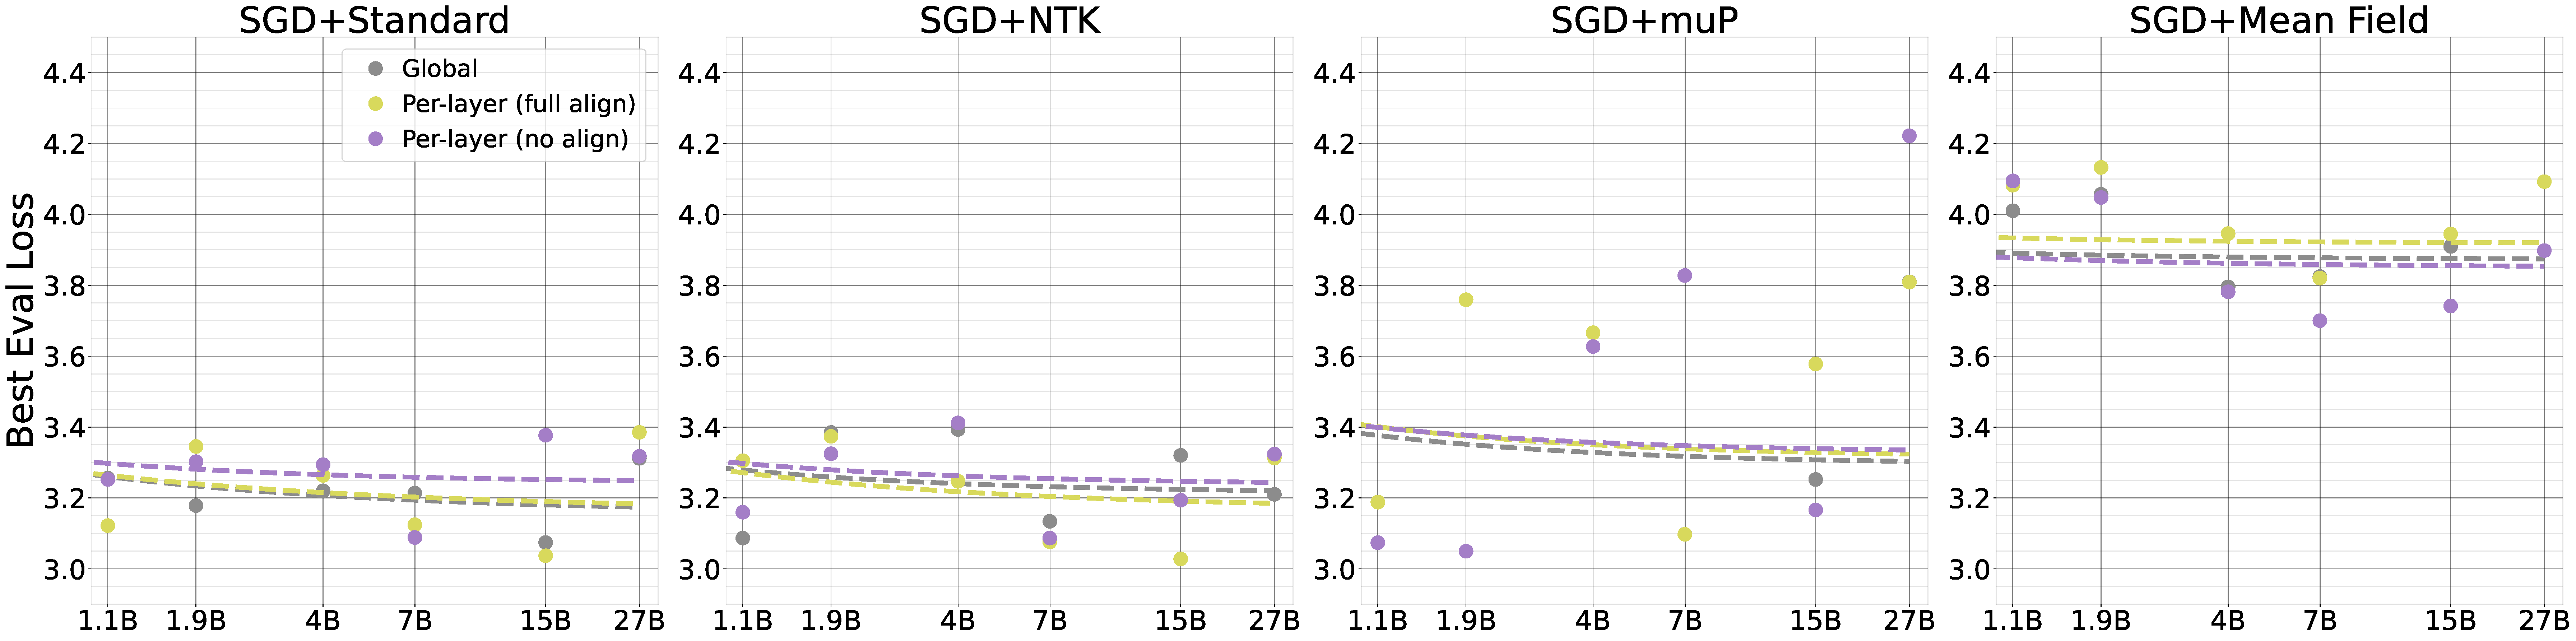
\includegraphics[width=\linewidth, trim={0, 0, 0, 0},clip]{icml2024/figures/per_layer_lr_appendix/sgd_appendix_grid.pdf}
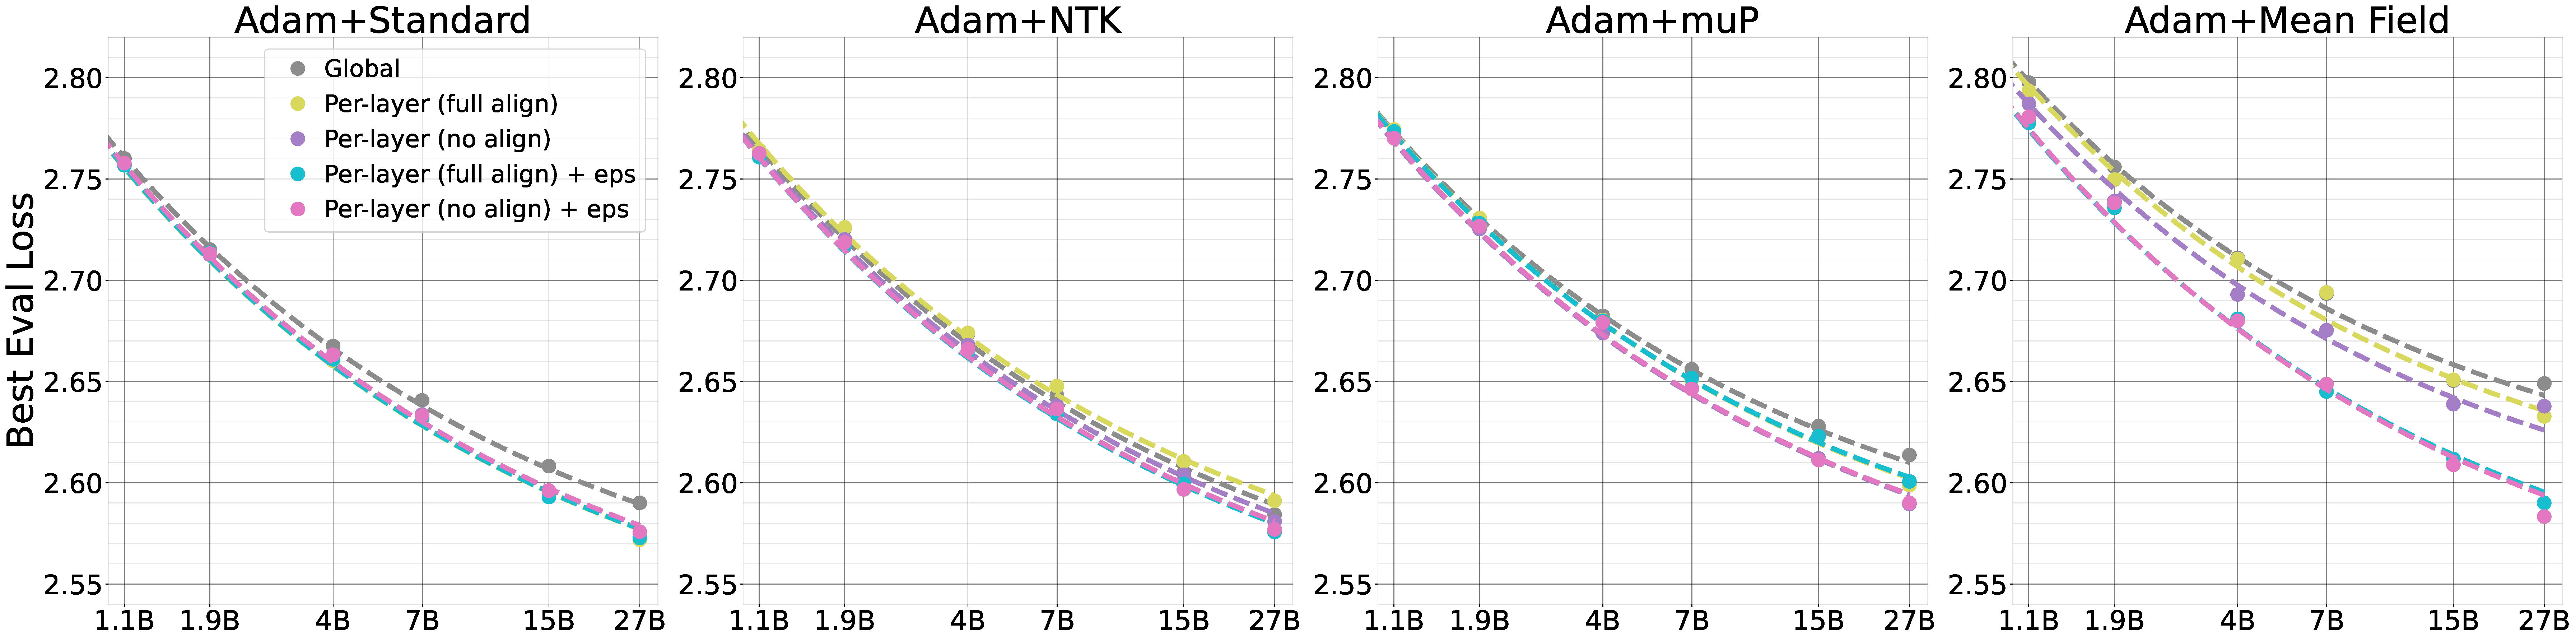
\includegraphics[width=\linewidth, trim={0, 0, 0, 0},clip]{icml2024/figures/per_layer_lr_appendix/adamw_appendix_grid.pdf}
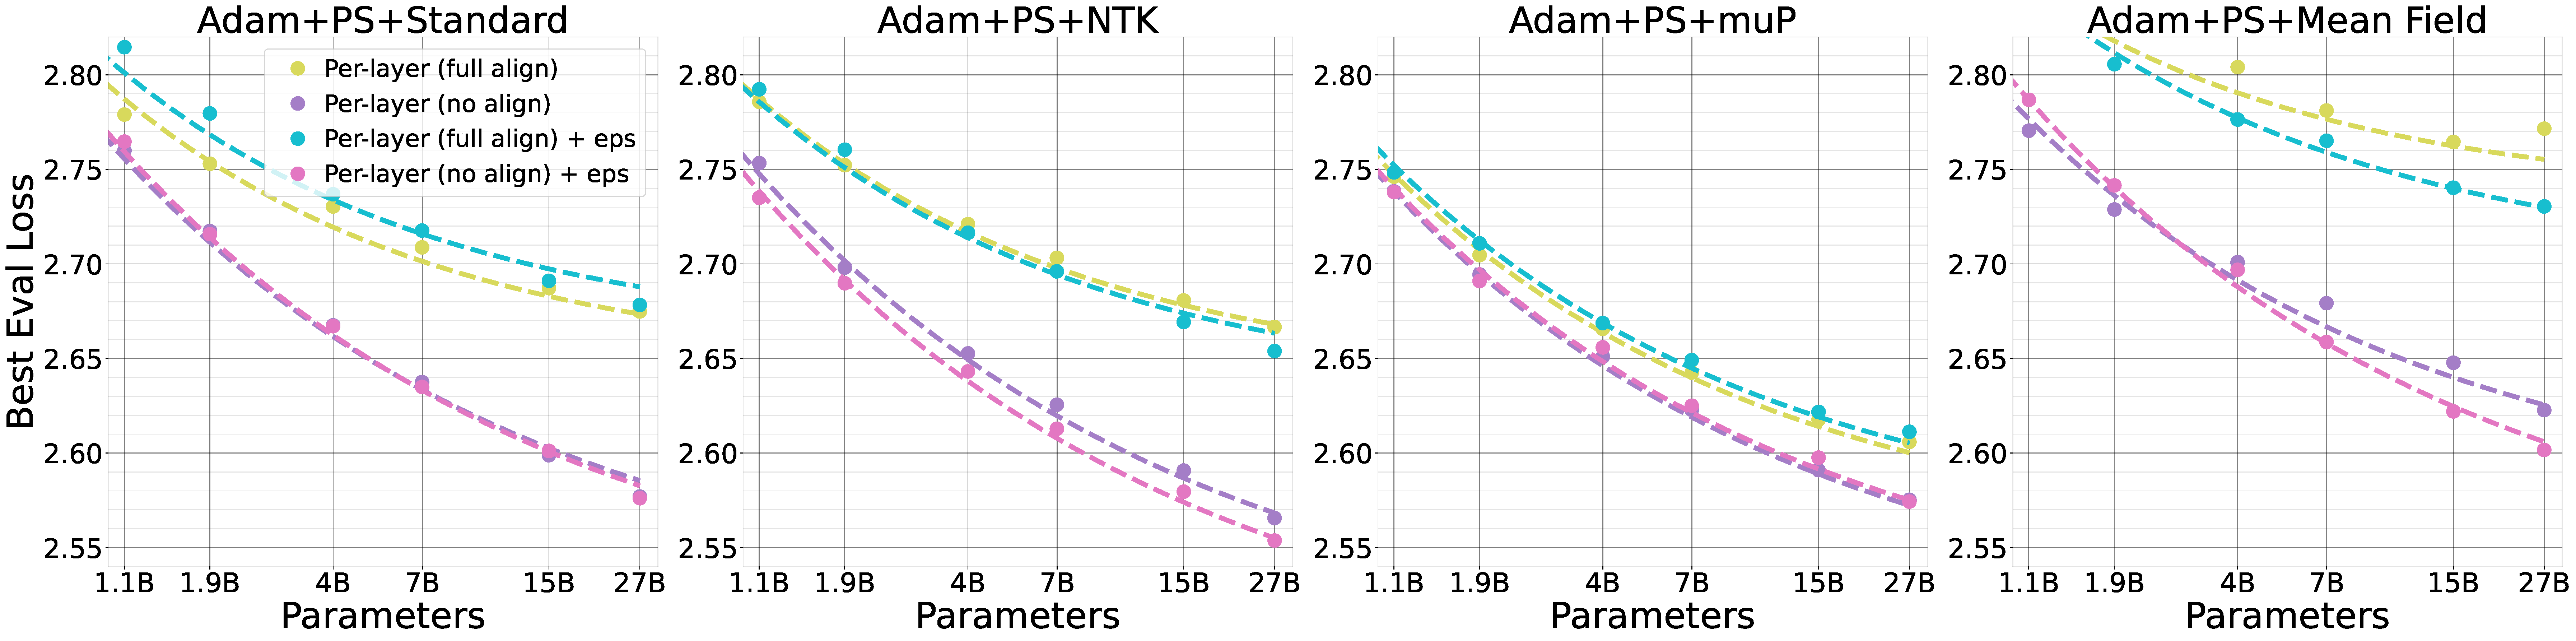
\includegraphics[width=\linewidth, trim={0, 0, 0, 0},clip]{icml2024/figures/per_layer_lr_appendix/adam_ps_appendix_grid.pdf}
\caption{Eval losses for the six largest model sizes for all settings with optimal constants. Rows = optimizers (SGD, Adam, Adam+parameter scaling), columns = parameterizations (standard, NTK, muP, Mean Field). Settings denoted "+eps" use per-layer epsilon with base epsilon = 1e-12. Note that Adam+parameter scaling global learning rate coincides with per-layer no alignment so there is no separate curve to show for global learning rates in the bottom row.}
\label{fig:app_scaling_optimal_constants}
\end{SidewaysFigure}
\clearpage

\thispagestyle{plain}
\begin{SidewaysFigure}
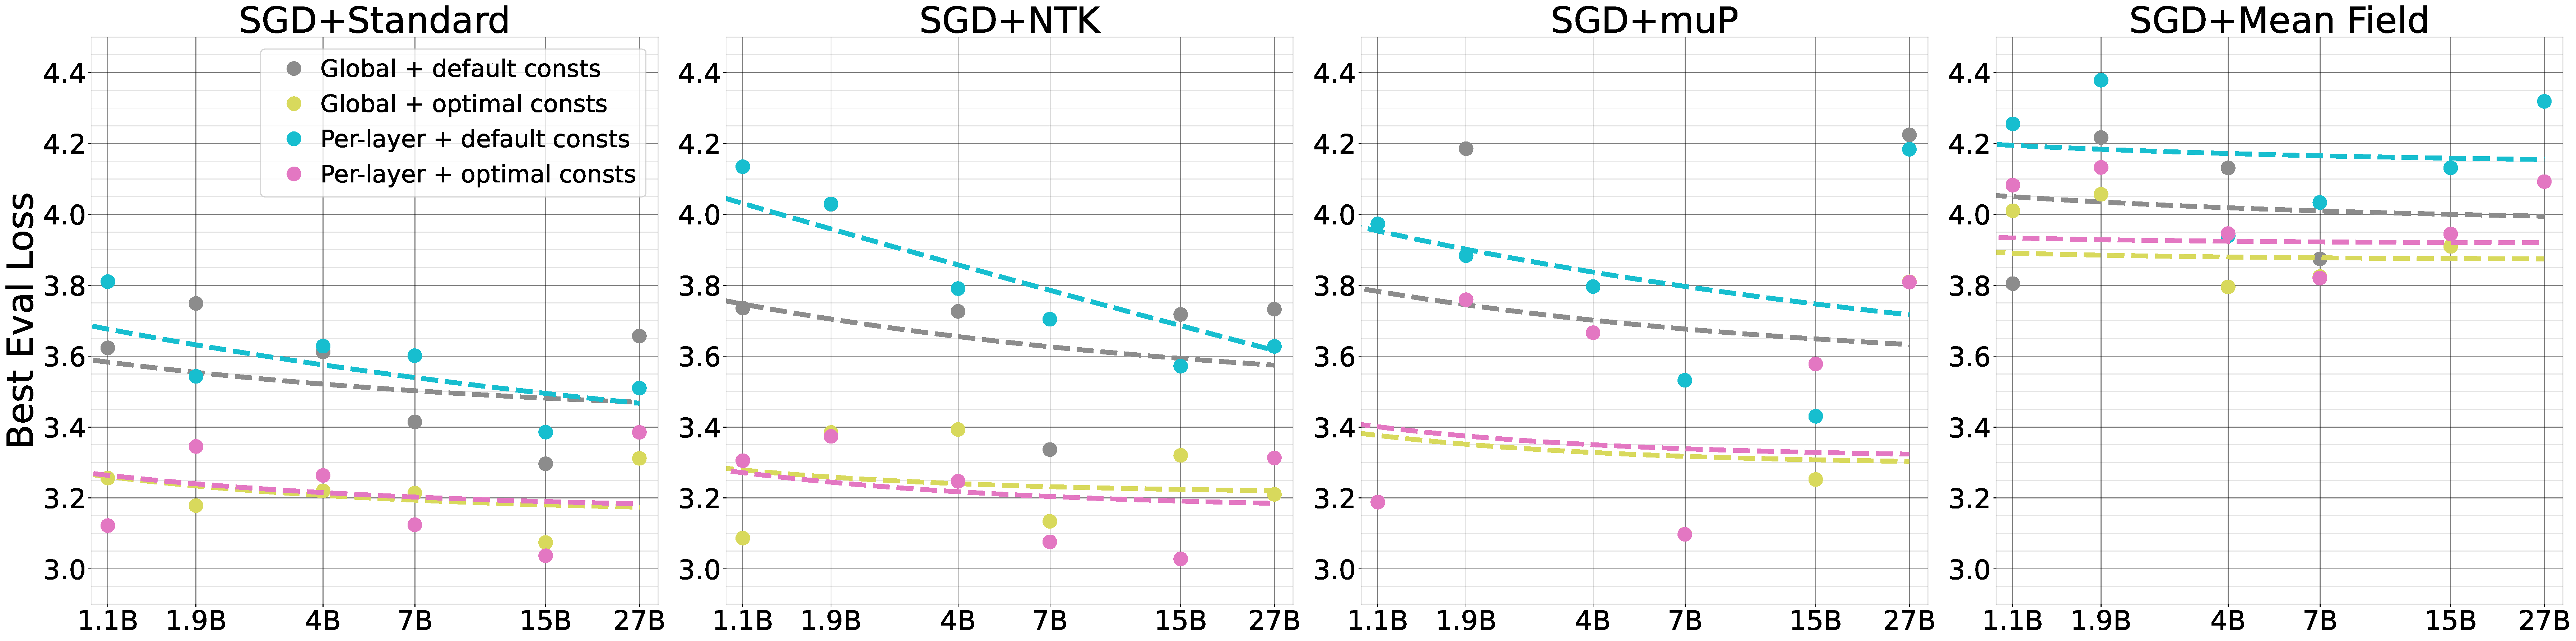
\includegraphics[width=\linewidth, trim={0, 0, 0, 0},clip]{icml2024/figures/per_layer_lr_appendix/sgd_ablation_appendix_grid.pdf}
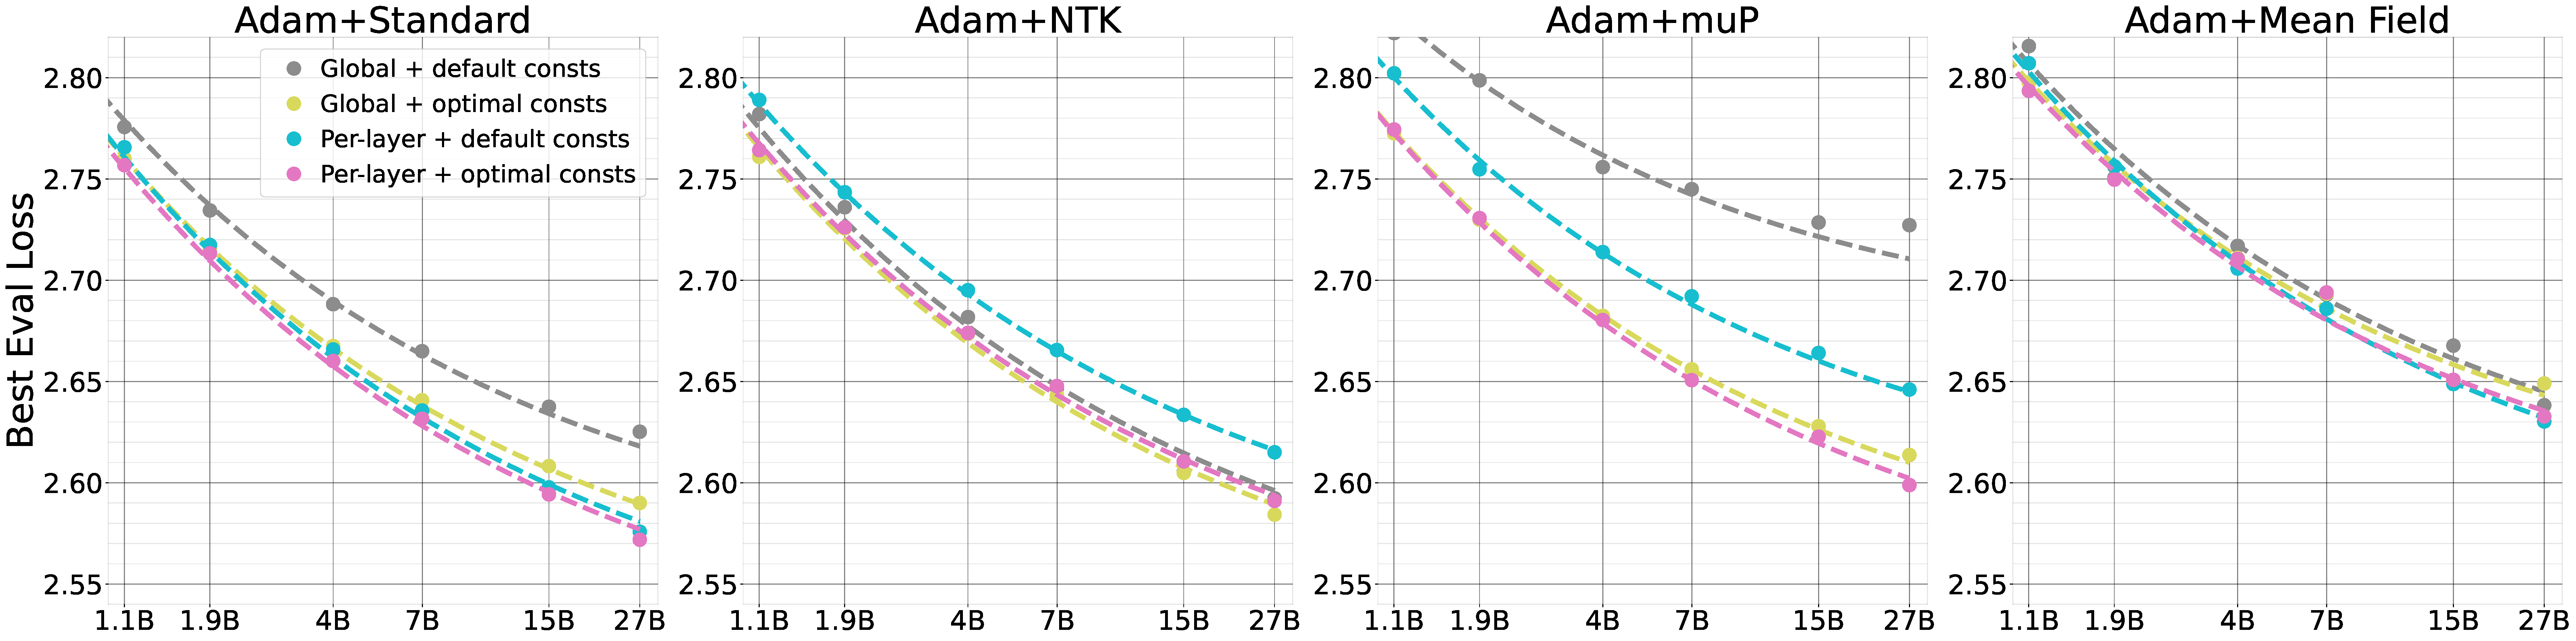
\includegraphics[width=\linewidth, trim={0, 0, 0, 0},clip]{icml2024/figures/per_layer_lr_appendix/adamw_ablation_appendix_grid.pdf}
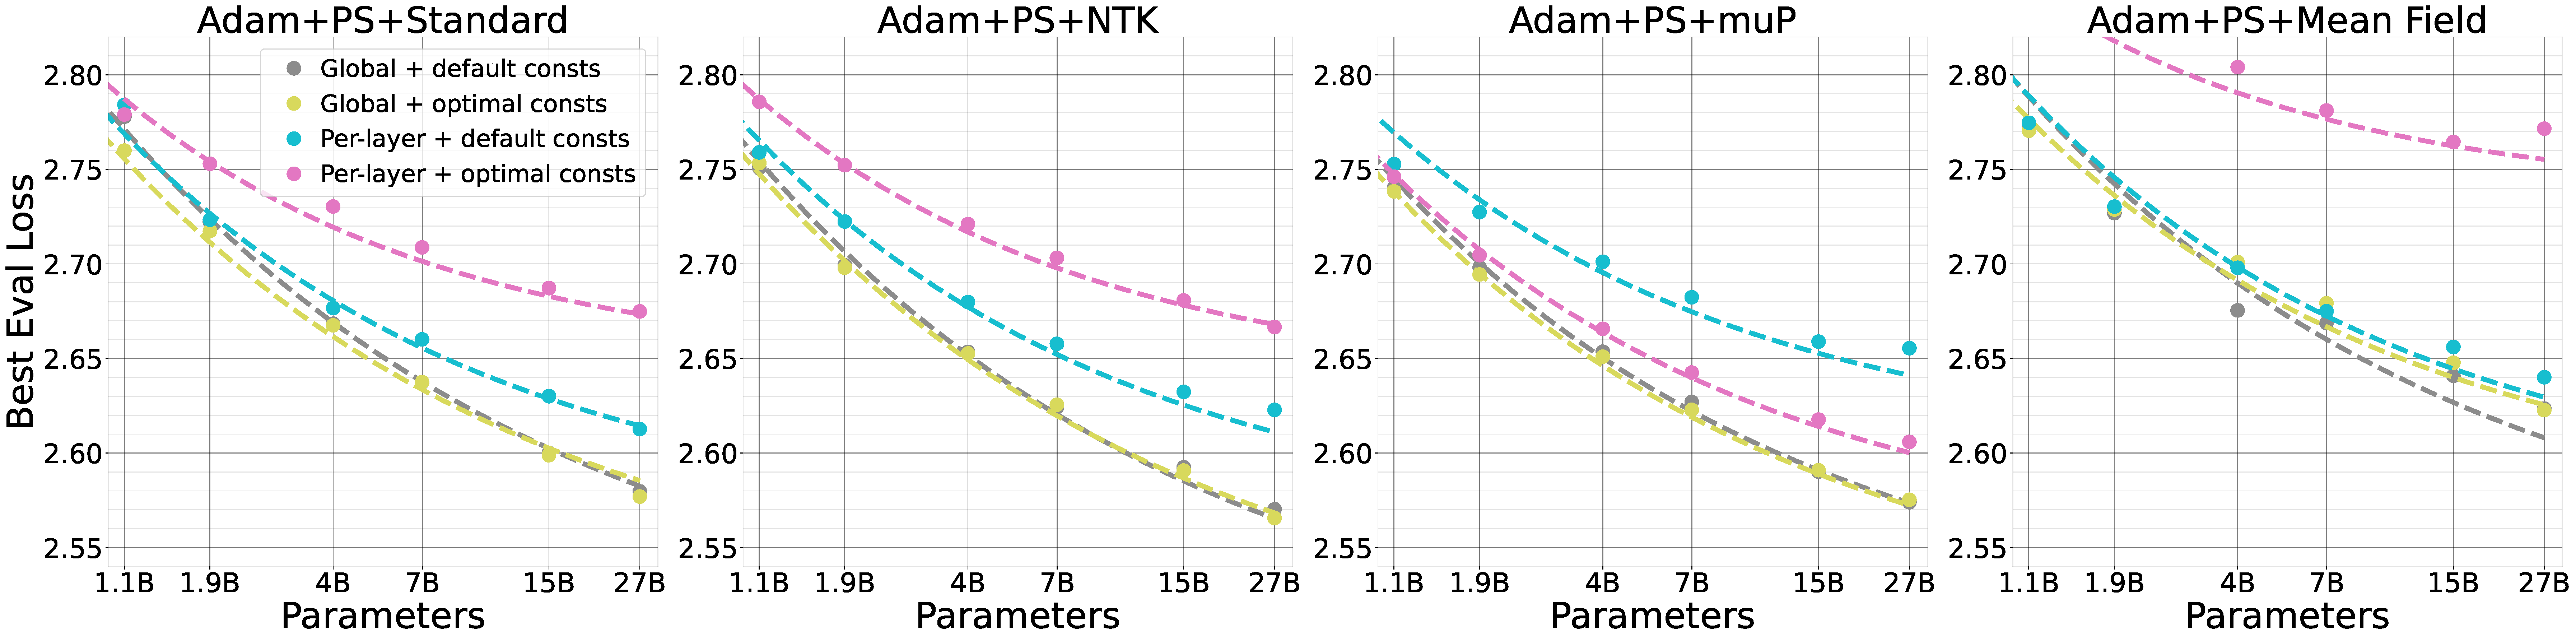
\includegraphics[width=\linewidth, trim={0, 0, 0, 0},clip]{icml2024/figures/per_layer_lr_appendix/adam_ps_ablation_appendix_grid.pdf}
\caption{Ablation showing eval losses for the six largest model sizes for all combinations of global or per-layer (full alignment) learning rates, and default or optimal constants. Rows = optimizers (SGD, Adam, Adam+parameter scaling), columns = parameterizations (standard, NTK, muP, Mean Field).}
\label{fig:app_scaling_ablation}
\end{SidewaysFigure}
\clearpage

\subsection{Additional Adam Epsilon Experiments}

In this section, we include additional results for epsilon experiments across all parameterizations.

In \cref{fig:epsilon_appendix_heatmaps}, we show heatmaps from tuning epsilon on all parameterizations. For both the constant epsilon and per-layer epsilon settings, we perform a learning rate sweep at each model dim for each value of epsilon or base epsilon. Using the best eval loss from each learning rate sweep, the heatmaps compare the eval loss to the other values of epsilon within that epsilon setting for that parameterization and model size. That is, each heatmap entry is colored based on the absolute difference to the best eval loss of the six entries in its row.

These results show that all parameterizations are affected by the choice of epsilon, but that different parameterizations have both different optimal values and different levels of sensitivity to epsilon. In all parameterizations, a constant epsilon of 1e-30 is too small and harms performance for the largest $26.8B$ parameter model ($D = 16{,}384$). Similarly, for per-layer epsilon, a base epsilon of 1e-4 is too large and harms performance. Compared to standard parameterization, muP tolerates large values of epsilon better (e.g. per-layer epsilon with base epsilon = 1e-4) and is harmed more by very small value epsilon (e.g. constant epsilon = 1e-30). Mean-field parameterization is most sensitive to epsilon and has the most narrow range of epsilon values with good performance, for both the constant and per-layer epsilon settings. NTK is overall quite similar to standard parameterization, with the exception that it NTK performance is harmed slightly by the default constant value of 1e-9.

In \cref{fig:epsilon_appendix_scaling_plots}, we show the eval loss vs model size for all three epsilon mitigations (constant epsilon = 1e-15, per-layer epsilon with base epsilon = 1e-12, and \emph{Adam-atan2}) compared against the baseline with the default constant epsilon of 1e-9 in all parameterizations. All three epsilon mitigations result in similar performance improvements, with different parameterizations having different sensitivity. Both standard and muP perform well with the default constant value of epsilon (1e-9) in our model sizes and are not affected by any of the epsilon mitigations. NTK performance improves slightly and MFP performance improves more substantially with all of the epsilon mitigations.

\begin{figure*}[ht]
    \begin{center}
        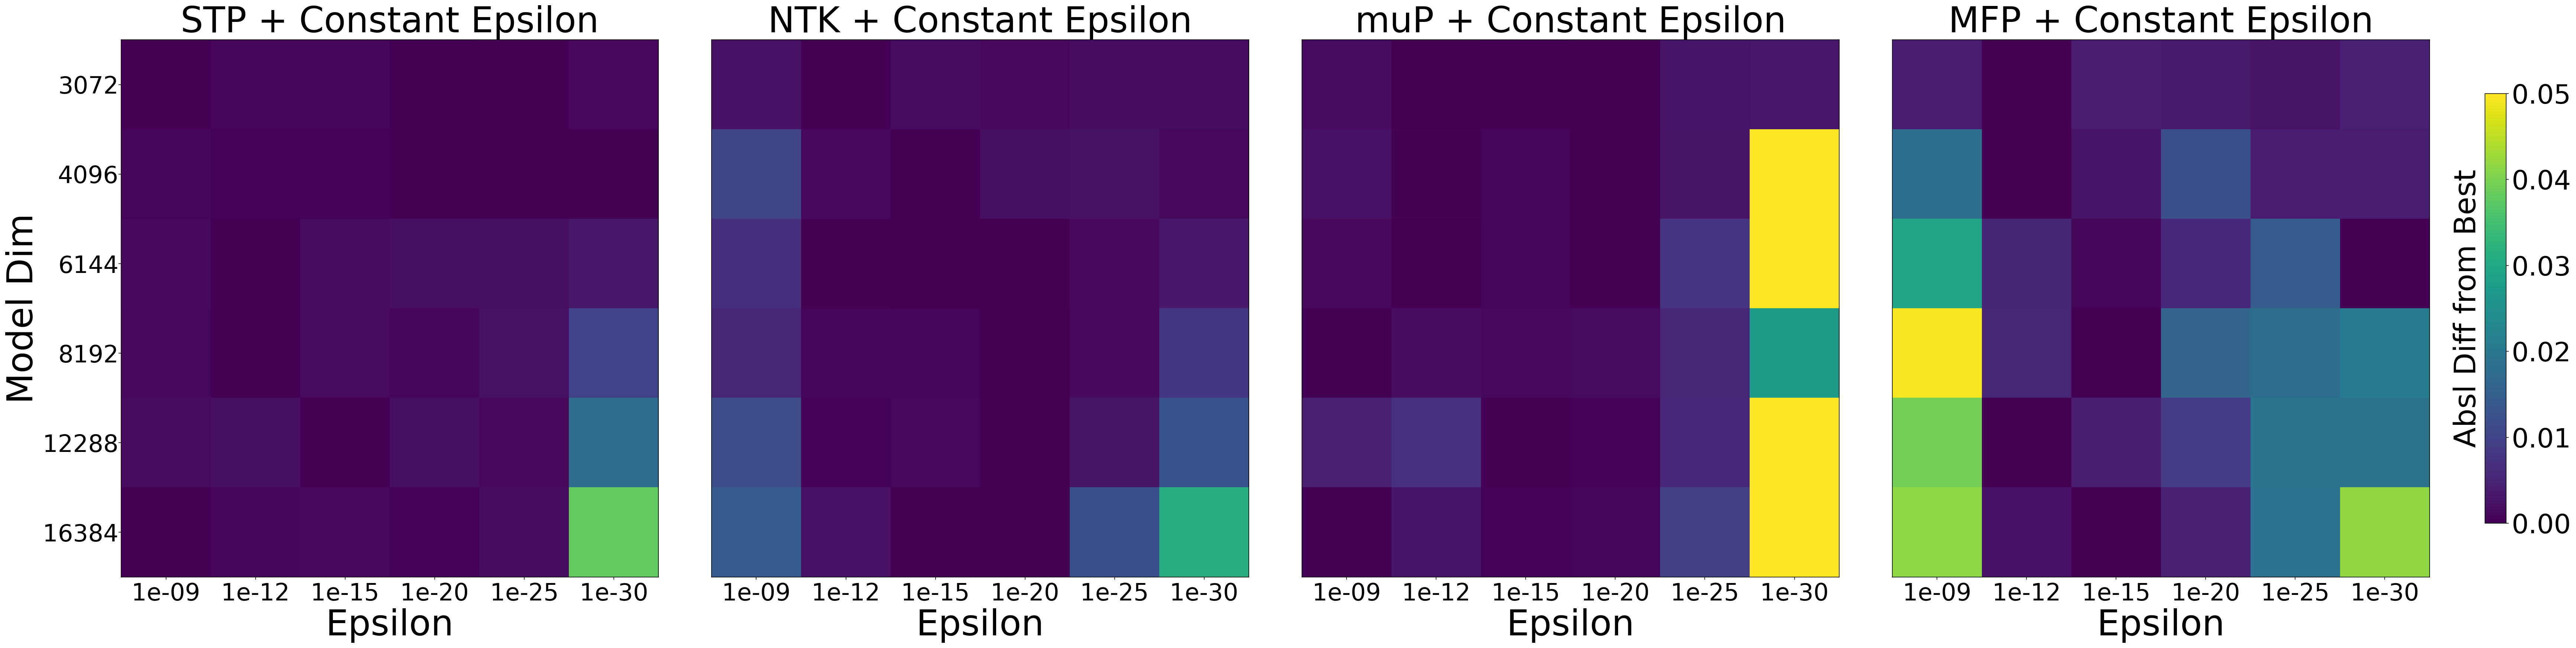
\includegraphics[width=\linewidth, trim={0, 0, 0, 0},clip]{icml2024/figures/epsilon/appendix_heatmaps/constant_epsilon_heatmaps.png}
       
        \figvspace
       
        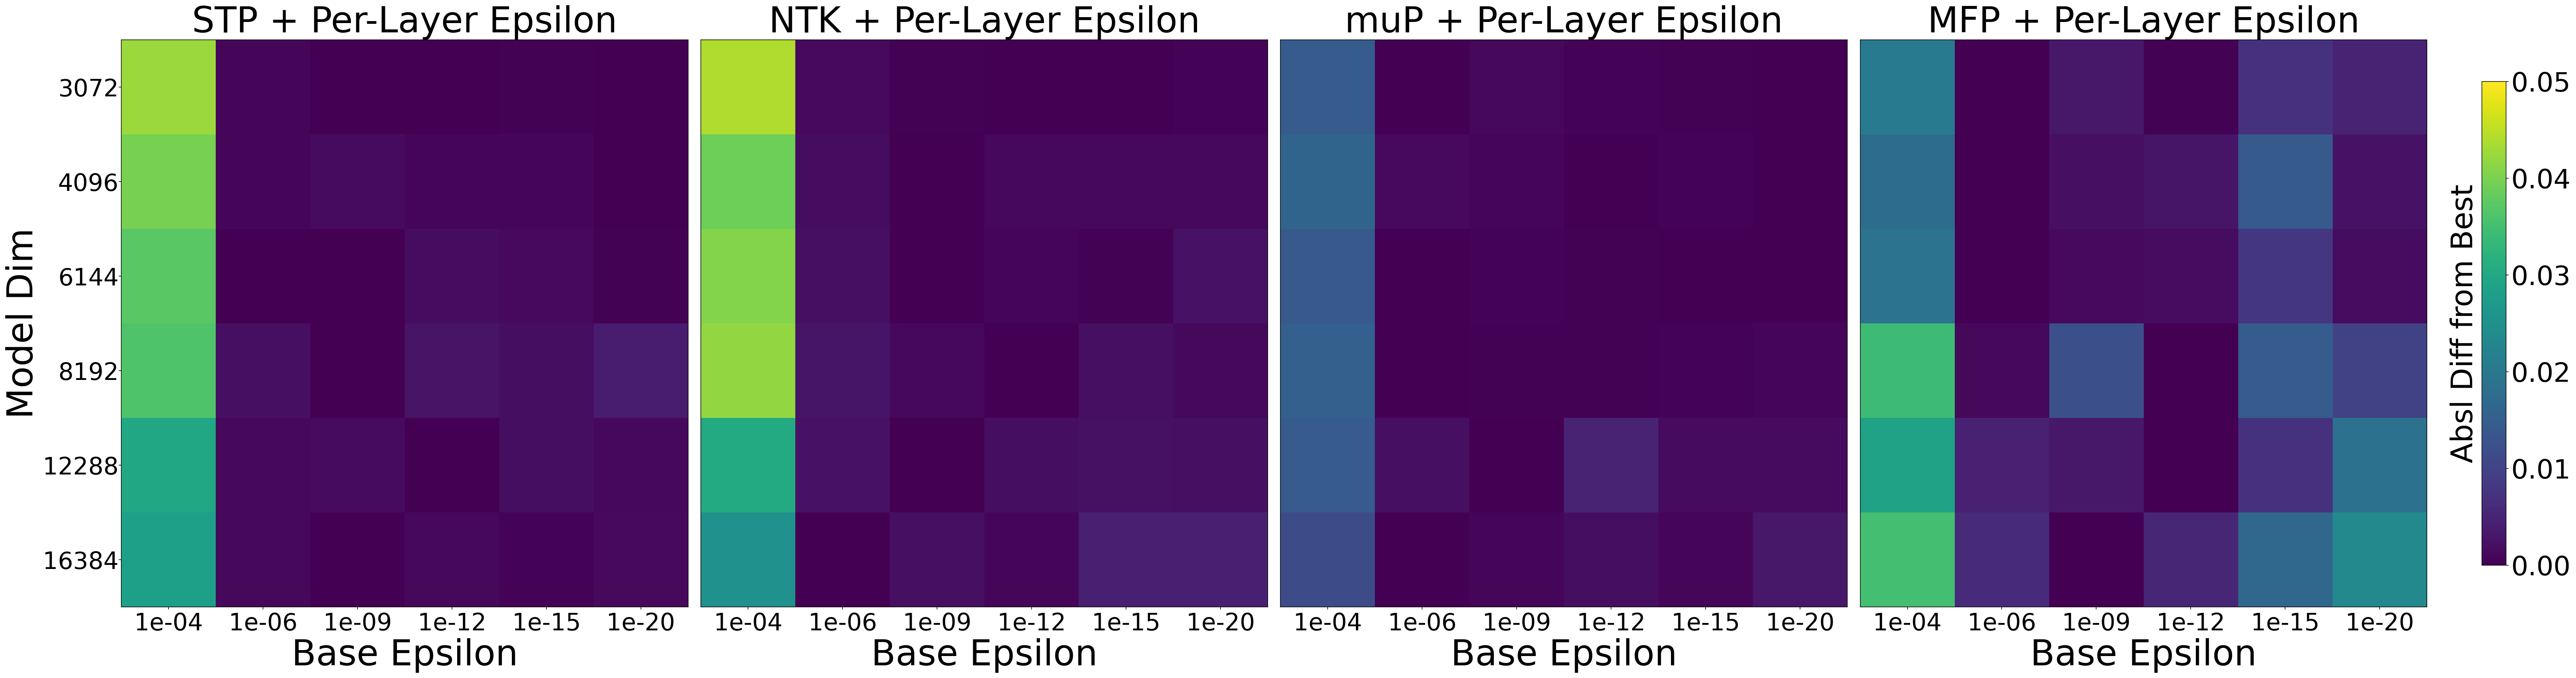
\includegraphics[width=\linewidth, trim={0, 0, 0, 0},clip]{icml2024/figures/epsilon/appendix_heatmaps/per_layer_epsilon_heatmaps.png}
       
       
        \caption{\textbf{All parameterizations are affected by epsilon but different parameterizations have different levels of sensitivity and different optimal values.} All experiments use Adam + per-layer learning rates assuming full alignment + optimal constants. Top row = constant epsilon, bottom row = per-layer epsilon. Number of training steps = $50{,}000$.}
        \label{fig:epsilon_appendix_heatmaps}
        \vspace{-24pt}
    \end{center}
\end{figure*}


\begin{figure*}[ht]
    \begin{center}
        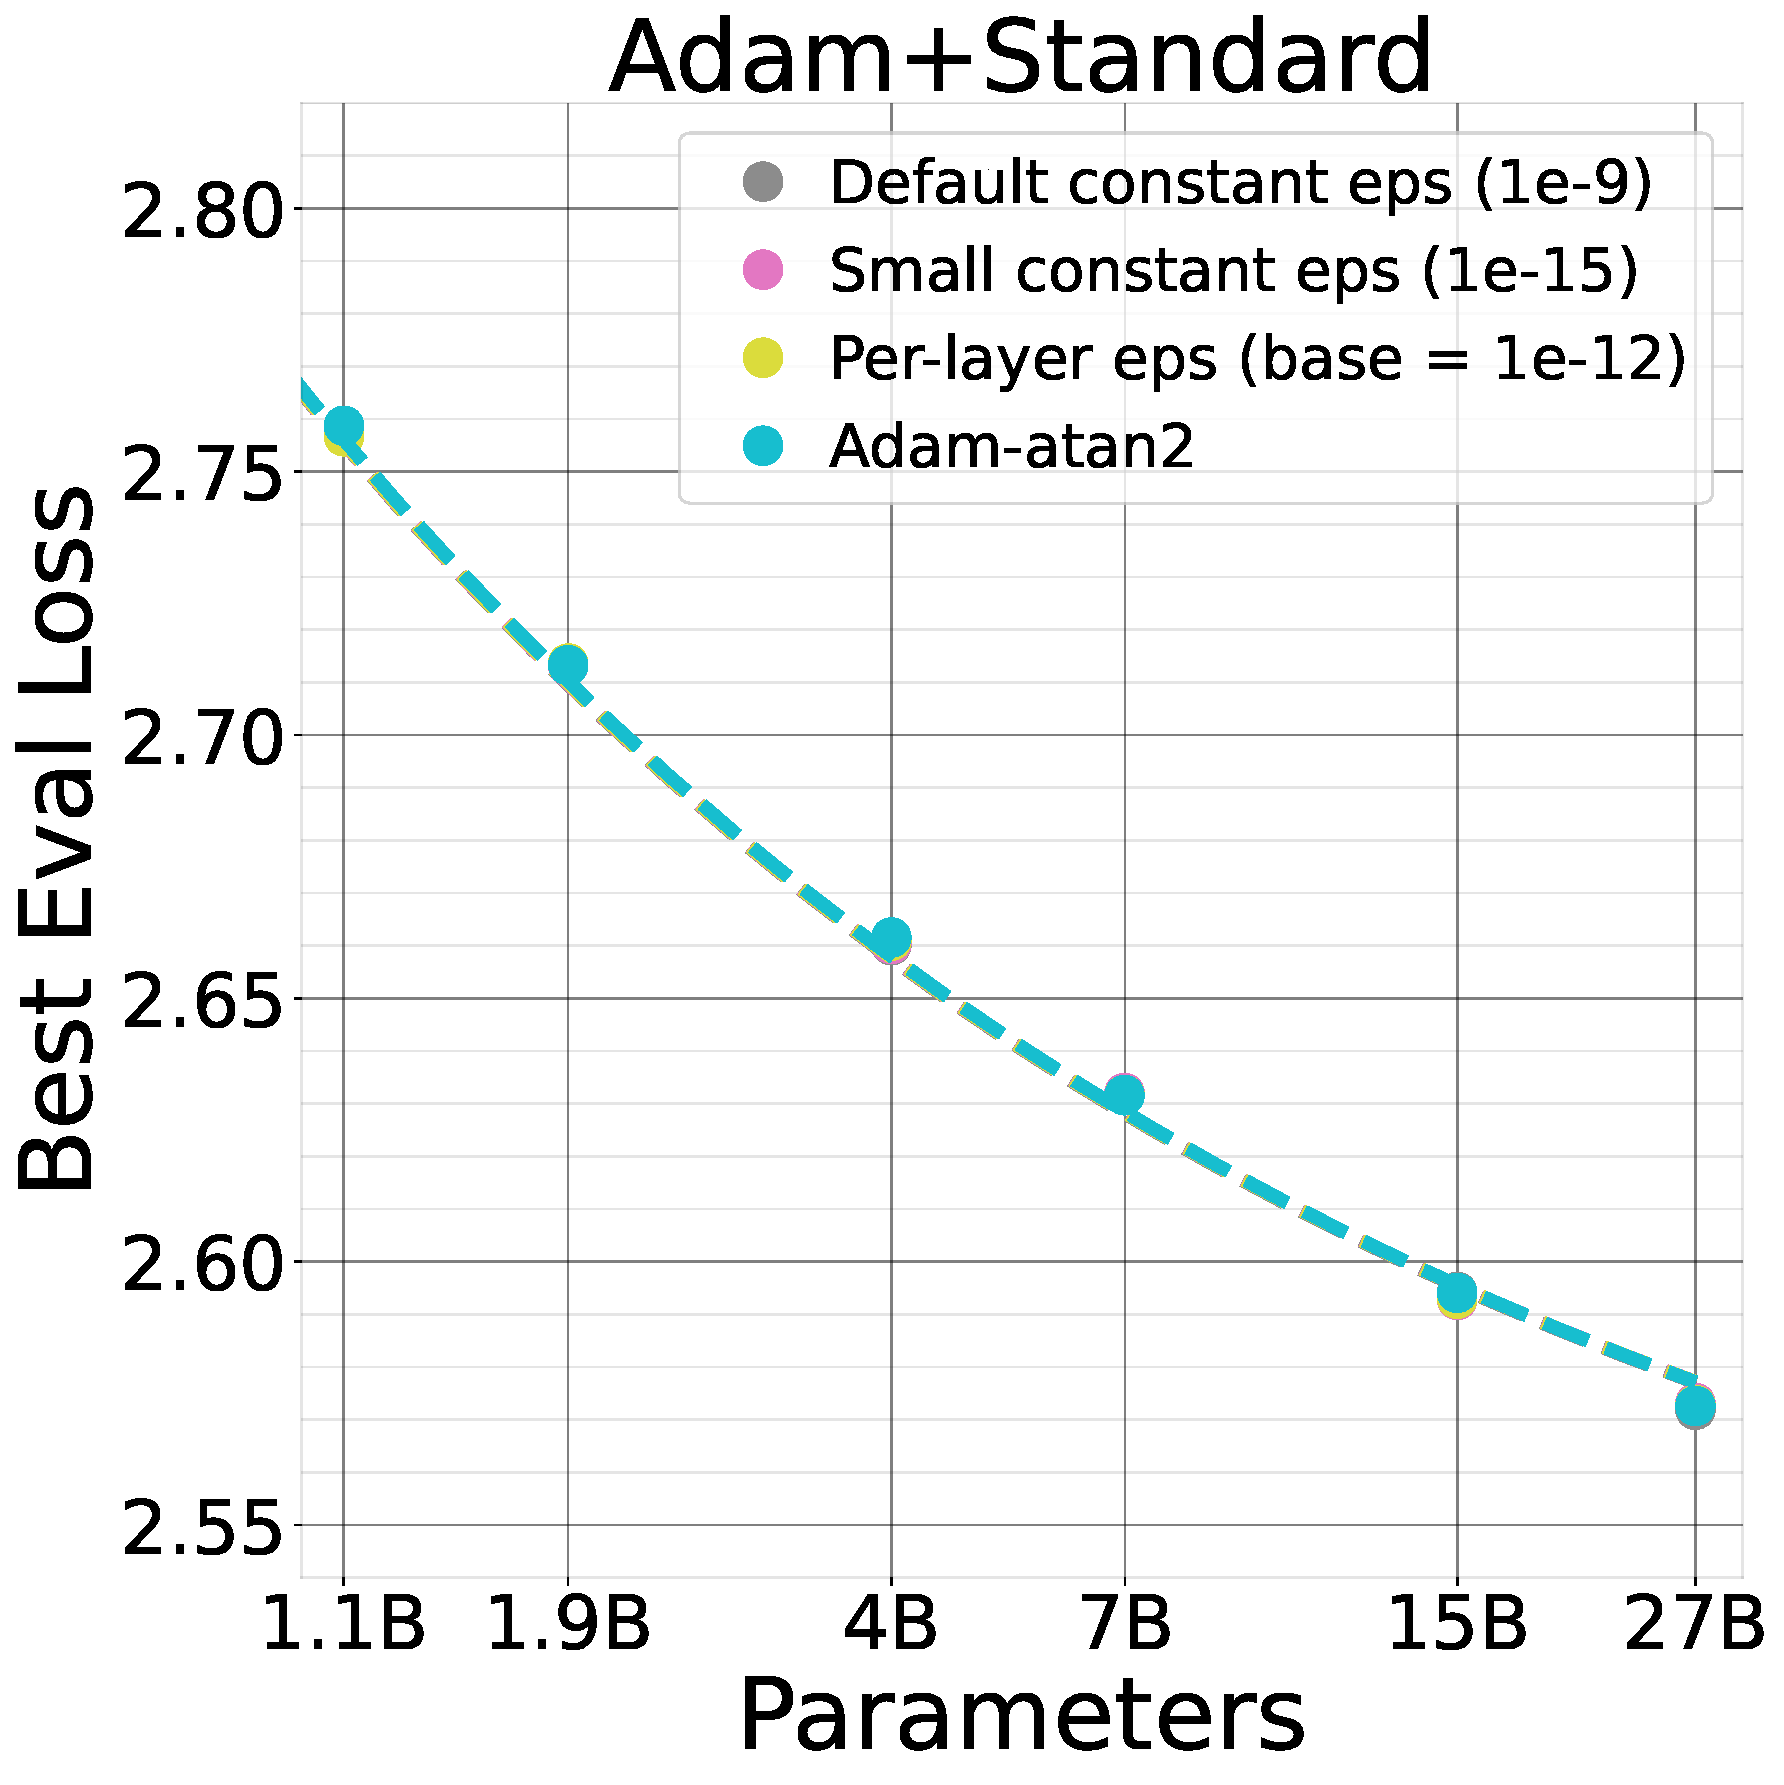
\includegraphics[width=0.48\linewidth, trim={0, 0, 0, 0},clip]{icml2024/figures/epsilon/stp_epsilon_eval_loss_comparisons_zoom6.pdf}
        \hfill
        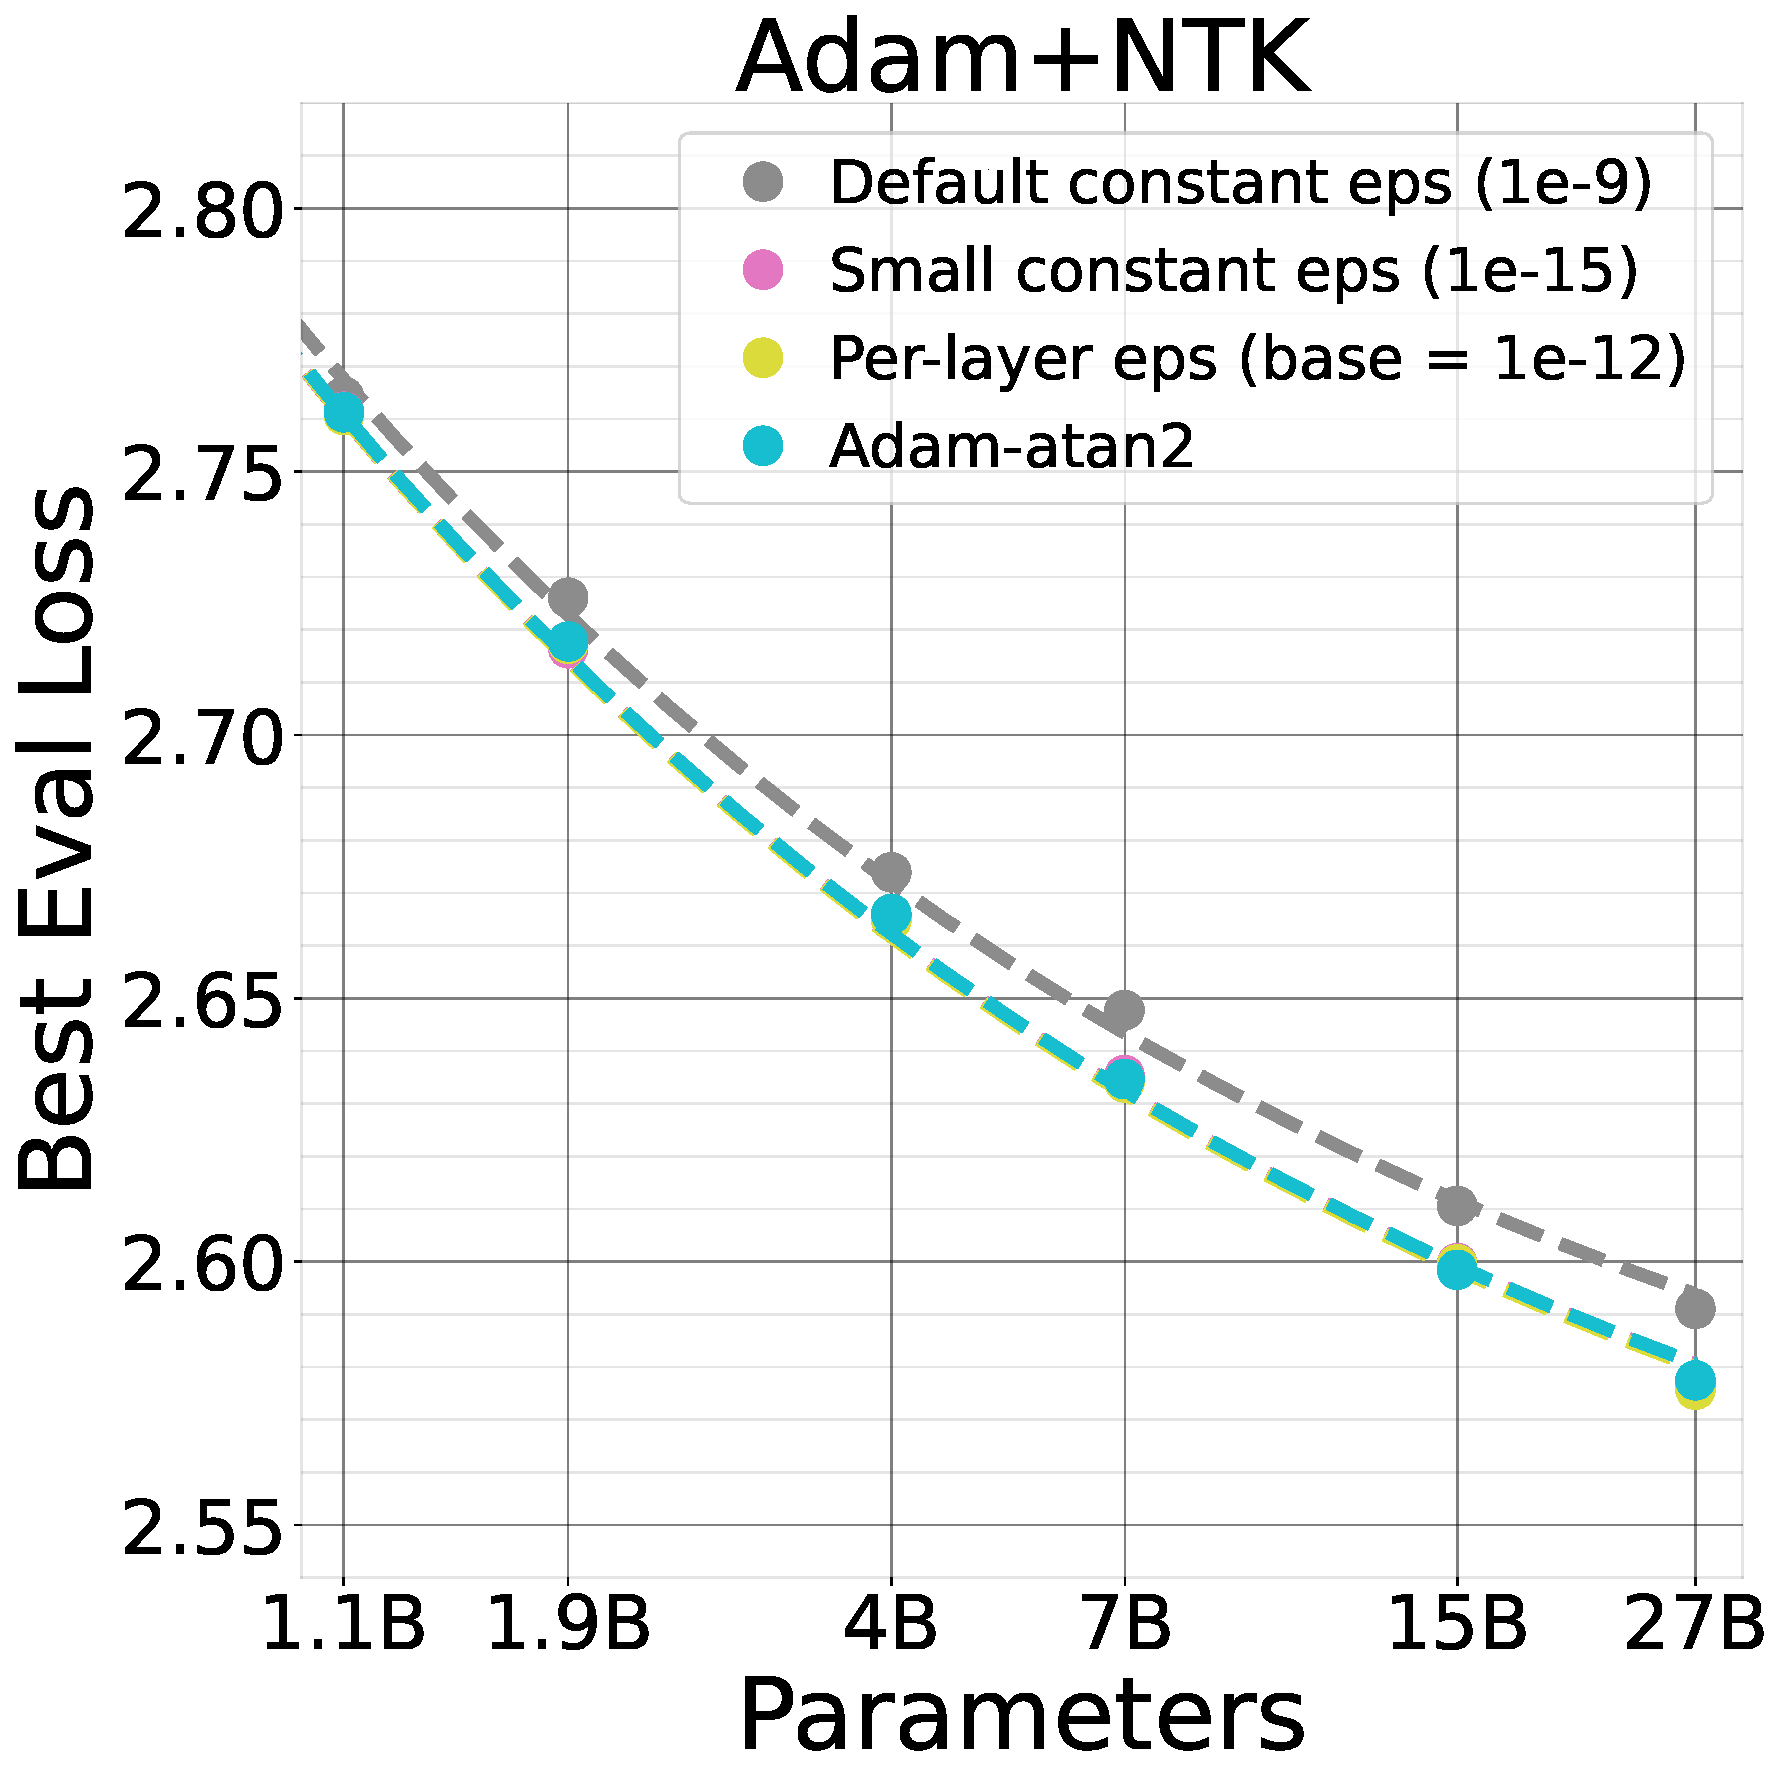
\includegraphics[width=0.48\linewidth, trim={0, 0, 0, 0},clip]{icml2024/figures/epsilon/ntk_epsilon_eval_loss_comparisons_zoom6.pdf}
       
        \figvspace
       
        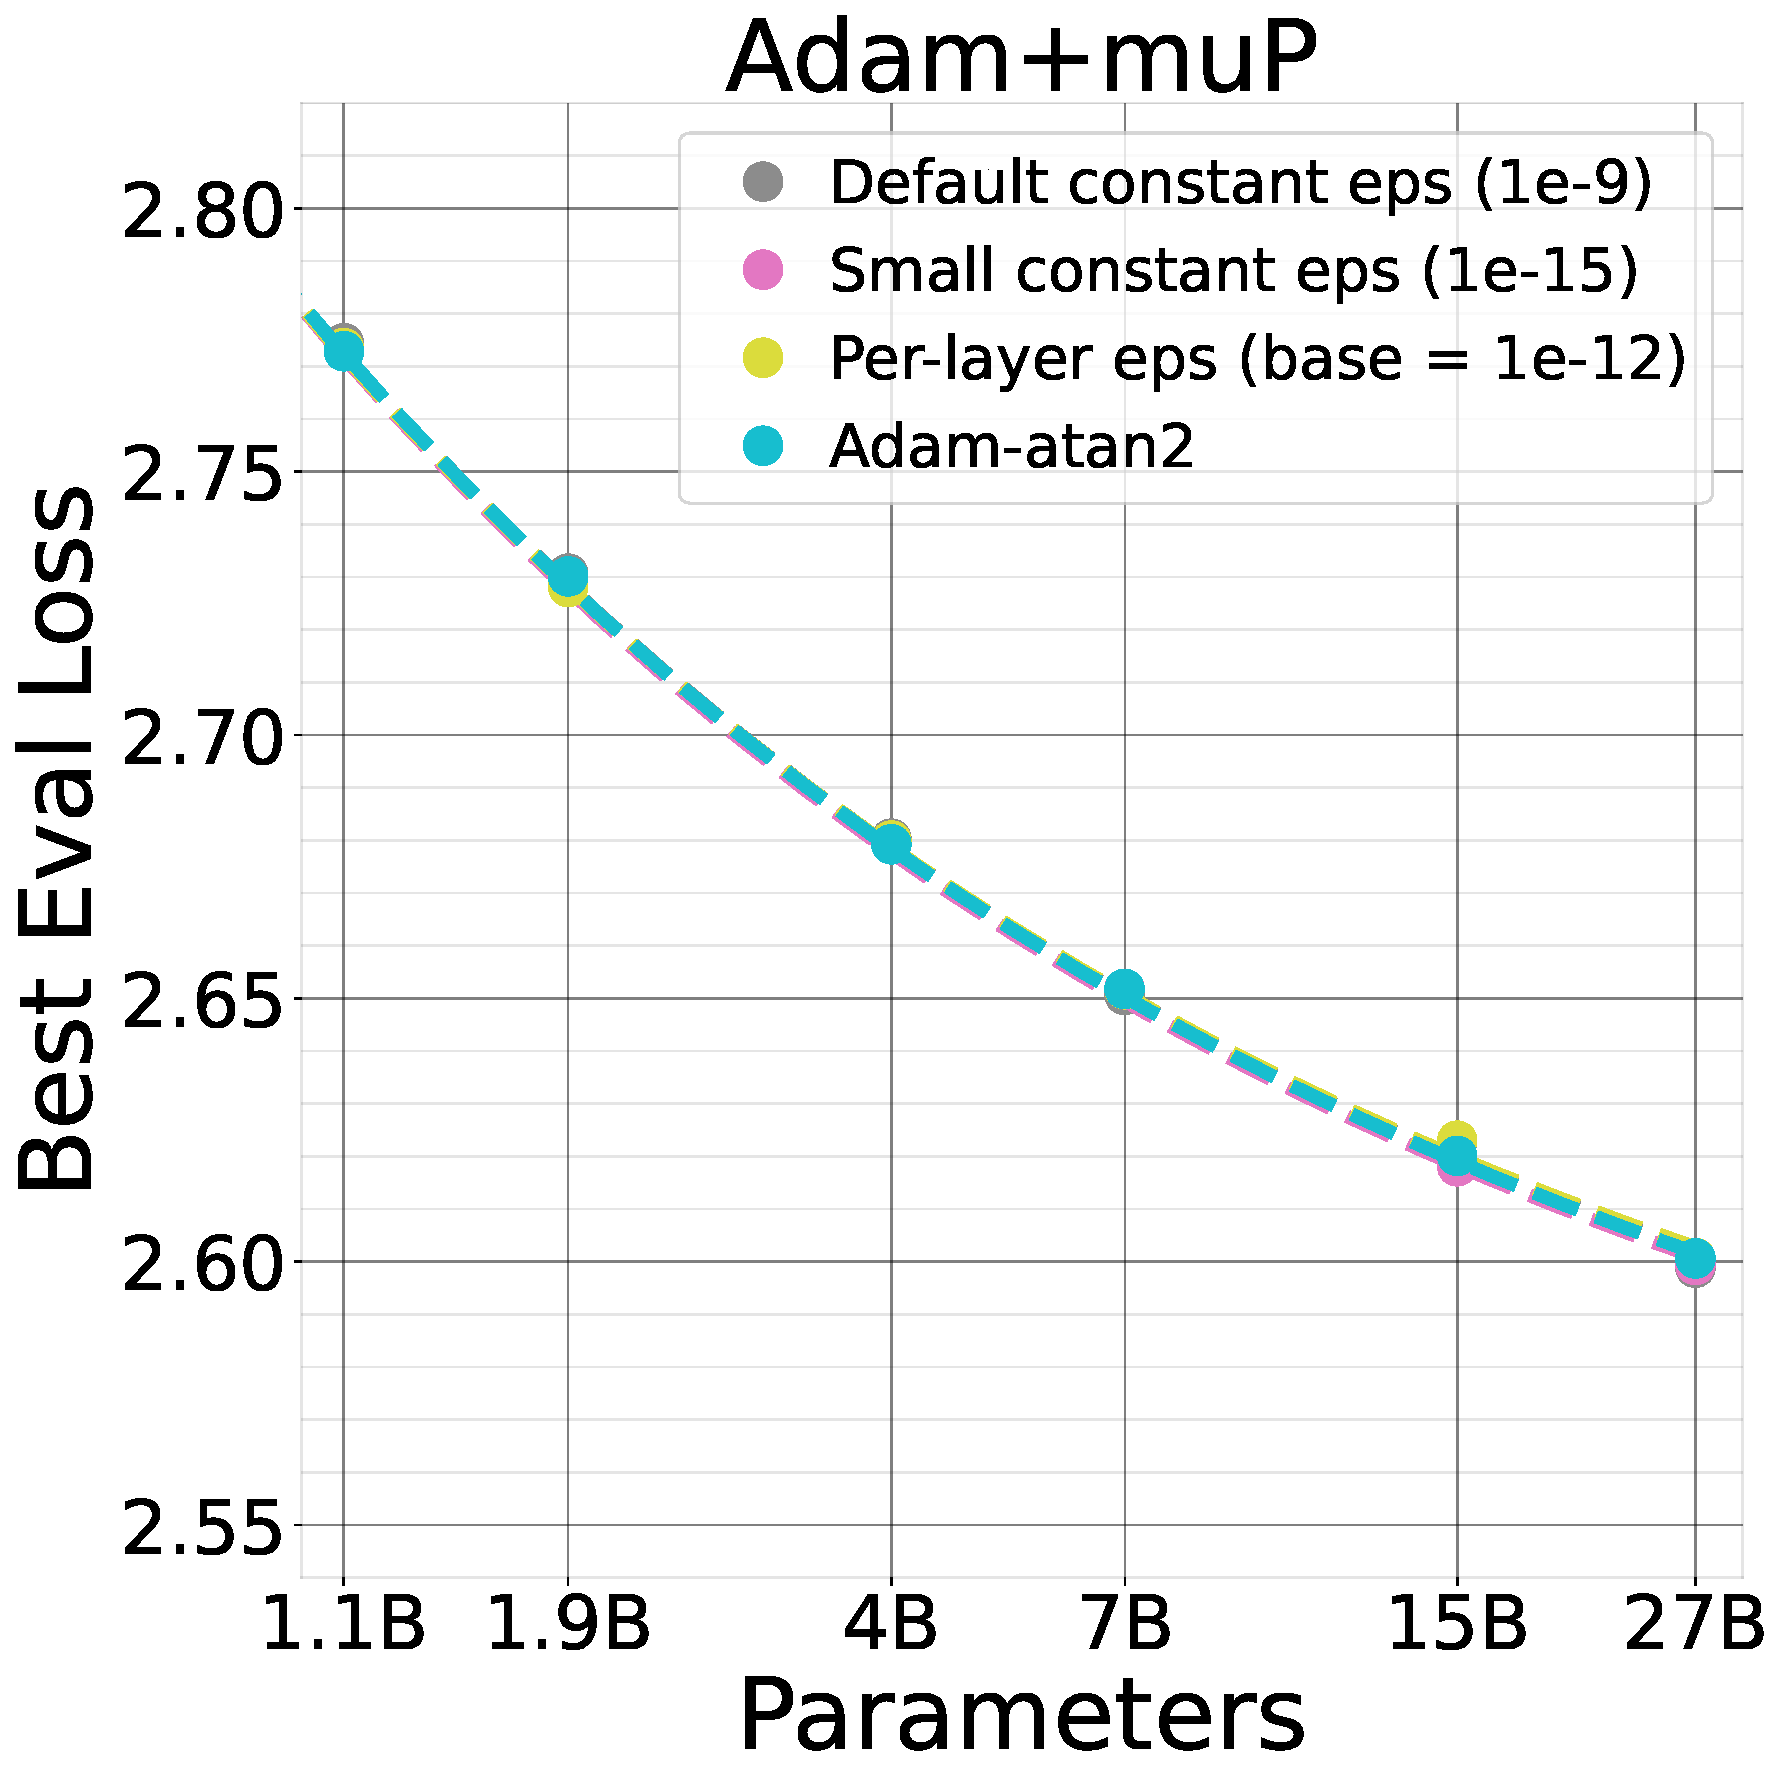
\includegraphics[width=0.48\linewidth, trim={0, 0, 0, 0},clip]{icml2024/figures/epsilon/mup_epsilon_eval_loss_comparisons_zoom6.pdf}
        \hfill
        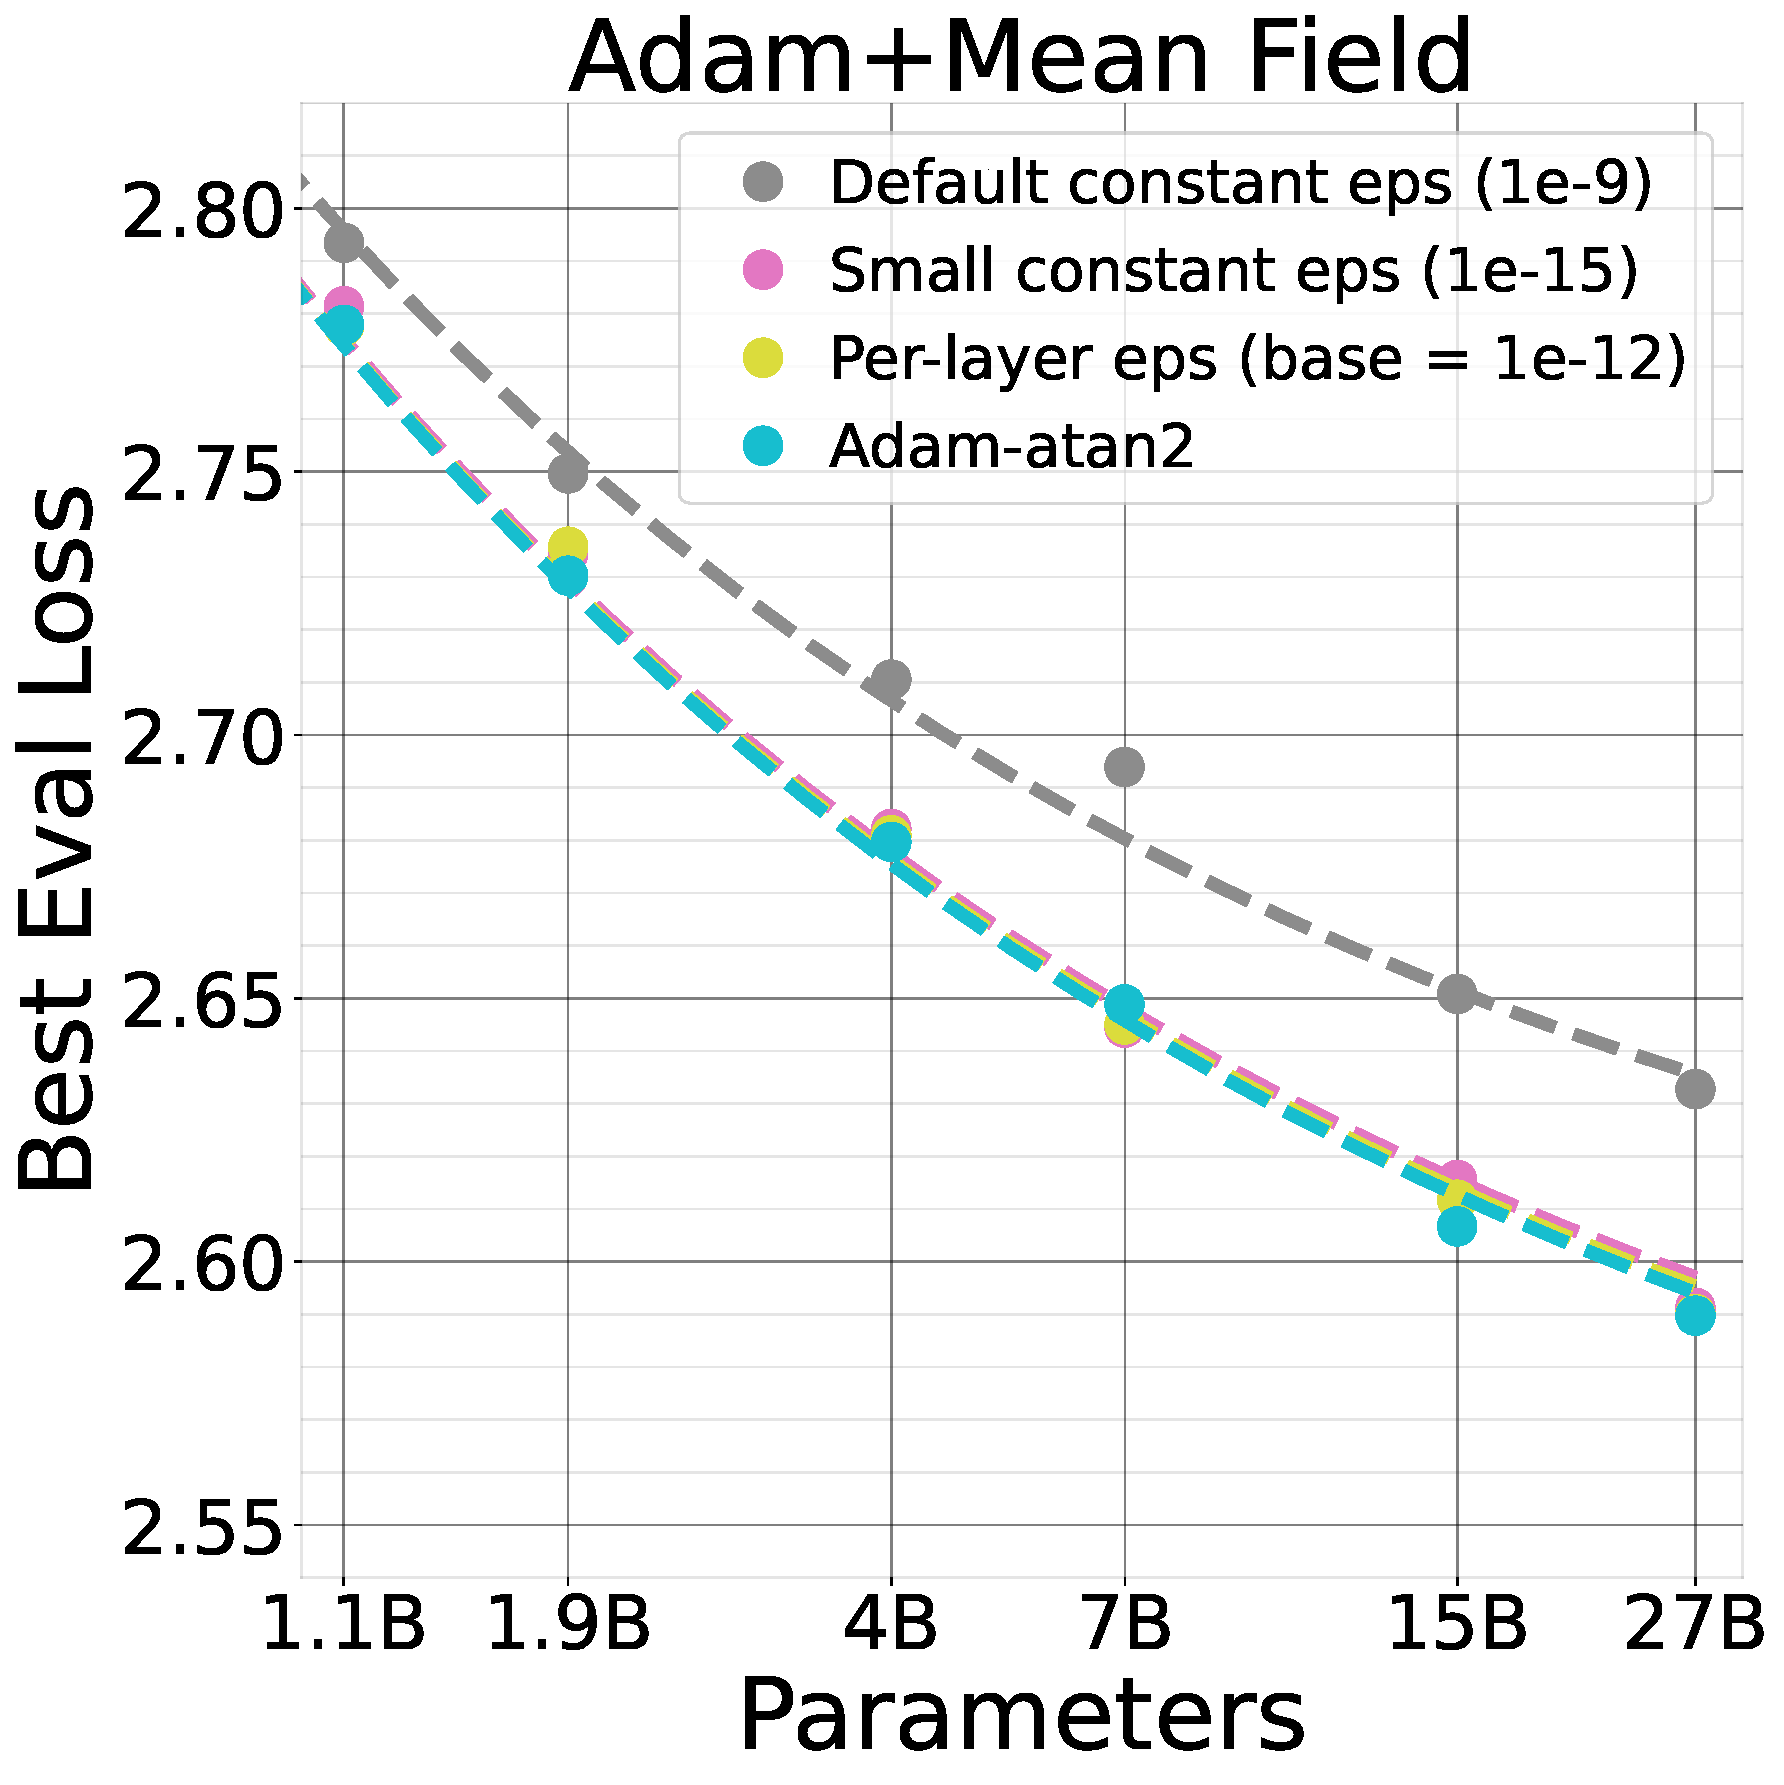
\includegraphics[width=0.48\linewidth, trim={0, 0, 0, 0},clip]{icml2024/figures/epsilon/mfp_epsilon_eval_loss_comparisons_zoom6.pdf}
       
       
        \caption{\textbf{All three epsilon mitigations similarly improve Adam performance on NTK and MFP, and do not change performance on STP and muP.} Experiments for all parameterizations comparing the three epsilon mitigations for Adam (small constant epsilon = 1e-15, per-layer epsilon with base epsilon = 1e-12, and Adam-atan2) to the baseline default constant epsilon of 1e-9.}
        \label{fig:epsilon_appendix_scaling_plots}
        \vspace{-24pt}
    \end{center}
\end{figure*}
\clearpage

\subsection{Weight Decay Experiments}
\label{app:weight_decay}
In current practice, weight decay is typically used for training large Transformers and may improve training stability by providing a small amount of regularization \citep{brown2020gpt3}. For the majority of our experiments, we do not use weight decay in order to reduce the number of possible confounding factors and focus our investigation on the impact of the parameterization and optimizer choices.

As a cross-check to ensure our conclusions are likely to transfer to settings with weight decay, we perform a set of experiments for Adam using per-layer learning rates assuming full alignment with a small constant weight decay of 1e-4, using ``decoupled" or ``independent" weight decay as proposed in AdamW \citep{loshchilov2018decoupled}. In decoupled weight decay, the weight decay is not scaled by the base learning rate; our value of 1e-4 decoupled weight decay corresponds to the higher values around 1e-2 or 1e-1 typically used for weight decay that does scale by the base learning rate.

Across parameterizations, with weight decay we see an improvement in the eval loss but similar learning rate scaling compared to the no weight decay setting. This suggests that while weight decay plays a beneficial role, it does not significantly alter the scaling behavior or have major parameterization-specific interactions and therefore we expect that our conclusions should transfer to settings with a small amount of weight decay. Learning rate sweeps for the weight decay experiments are included in  \cref{fig:appendix_adam_weight_decay}.

\vspace{48pt}

\begin{figure*}[ht]
    \begin{center}
        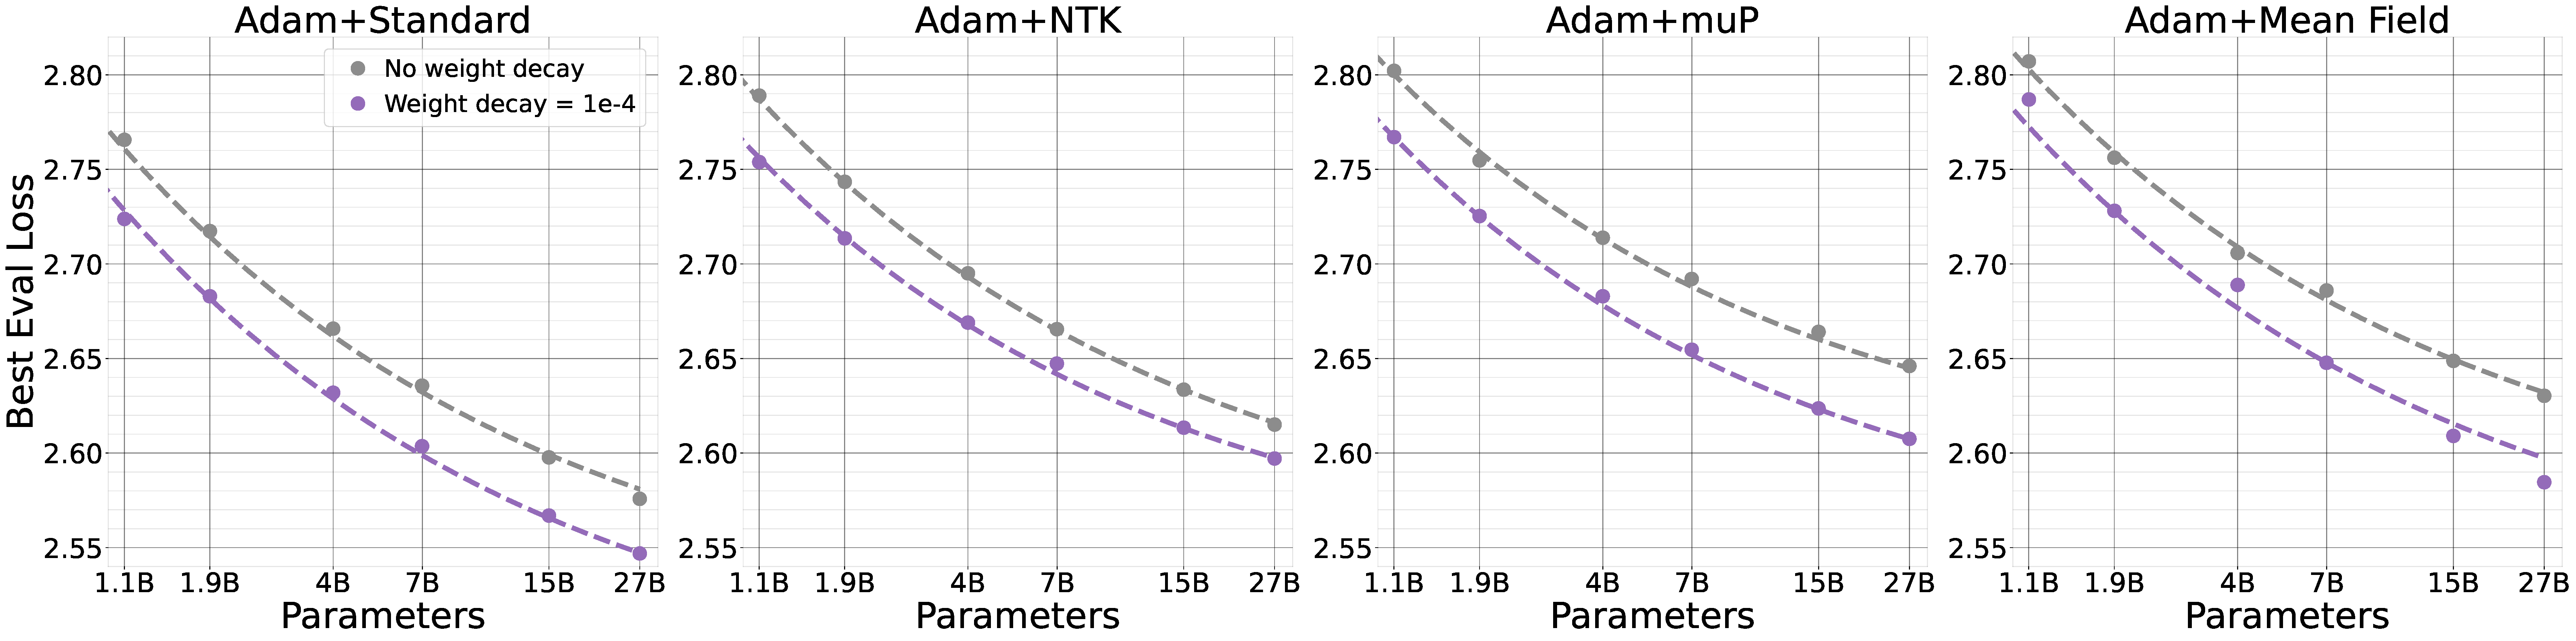
\includegraphics[width=\linewidth, trim={0, 0, 0, 0},clip]{icml2024/figures/wd_appendix/wd_per_module_lr_scaling_plot.pdf}
       
        \caption{\centering{\textbf{Weight decay = 1e-4 (decoupled) improves the eval loss for all parameterizations and model sizes but overall scaling behavior is similar.} All experiments use Adam + per-layer learning rates assuming full alignment + default constants. Number of training steps = $50{,}000$.}}
        \label{fig:wd_lr_sweeps}
    \end{center}
\end{figure*}

\vfill

\clearpage
\thispagestyle{plain}
\begin{SidewaysFigure}
        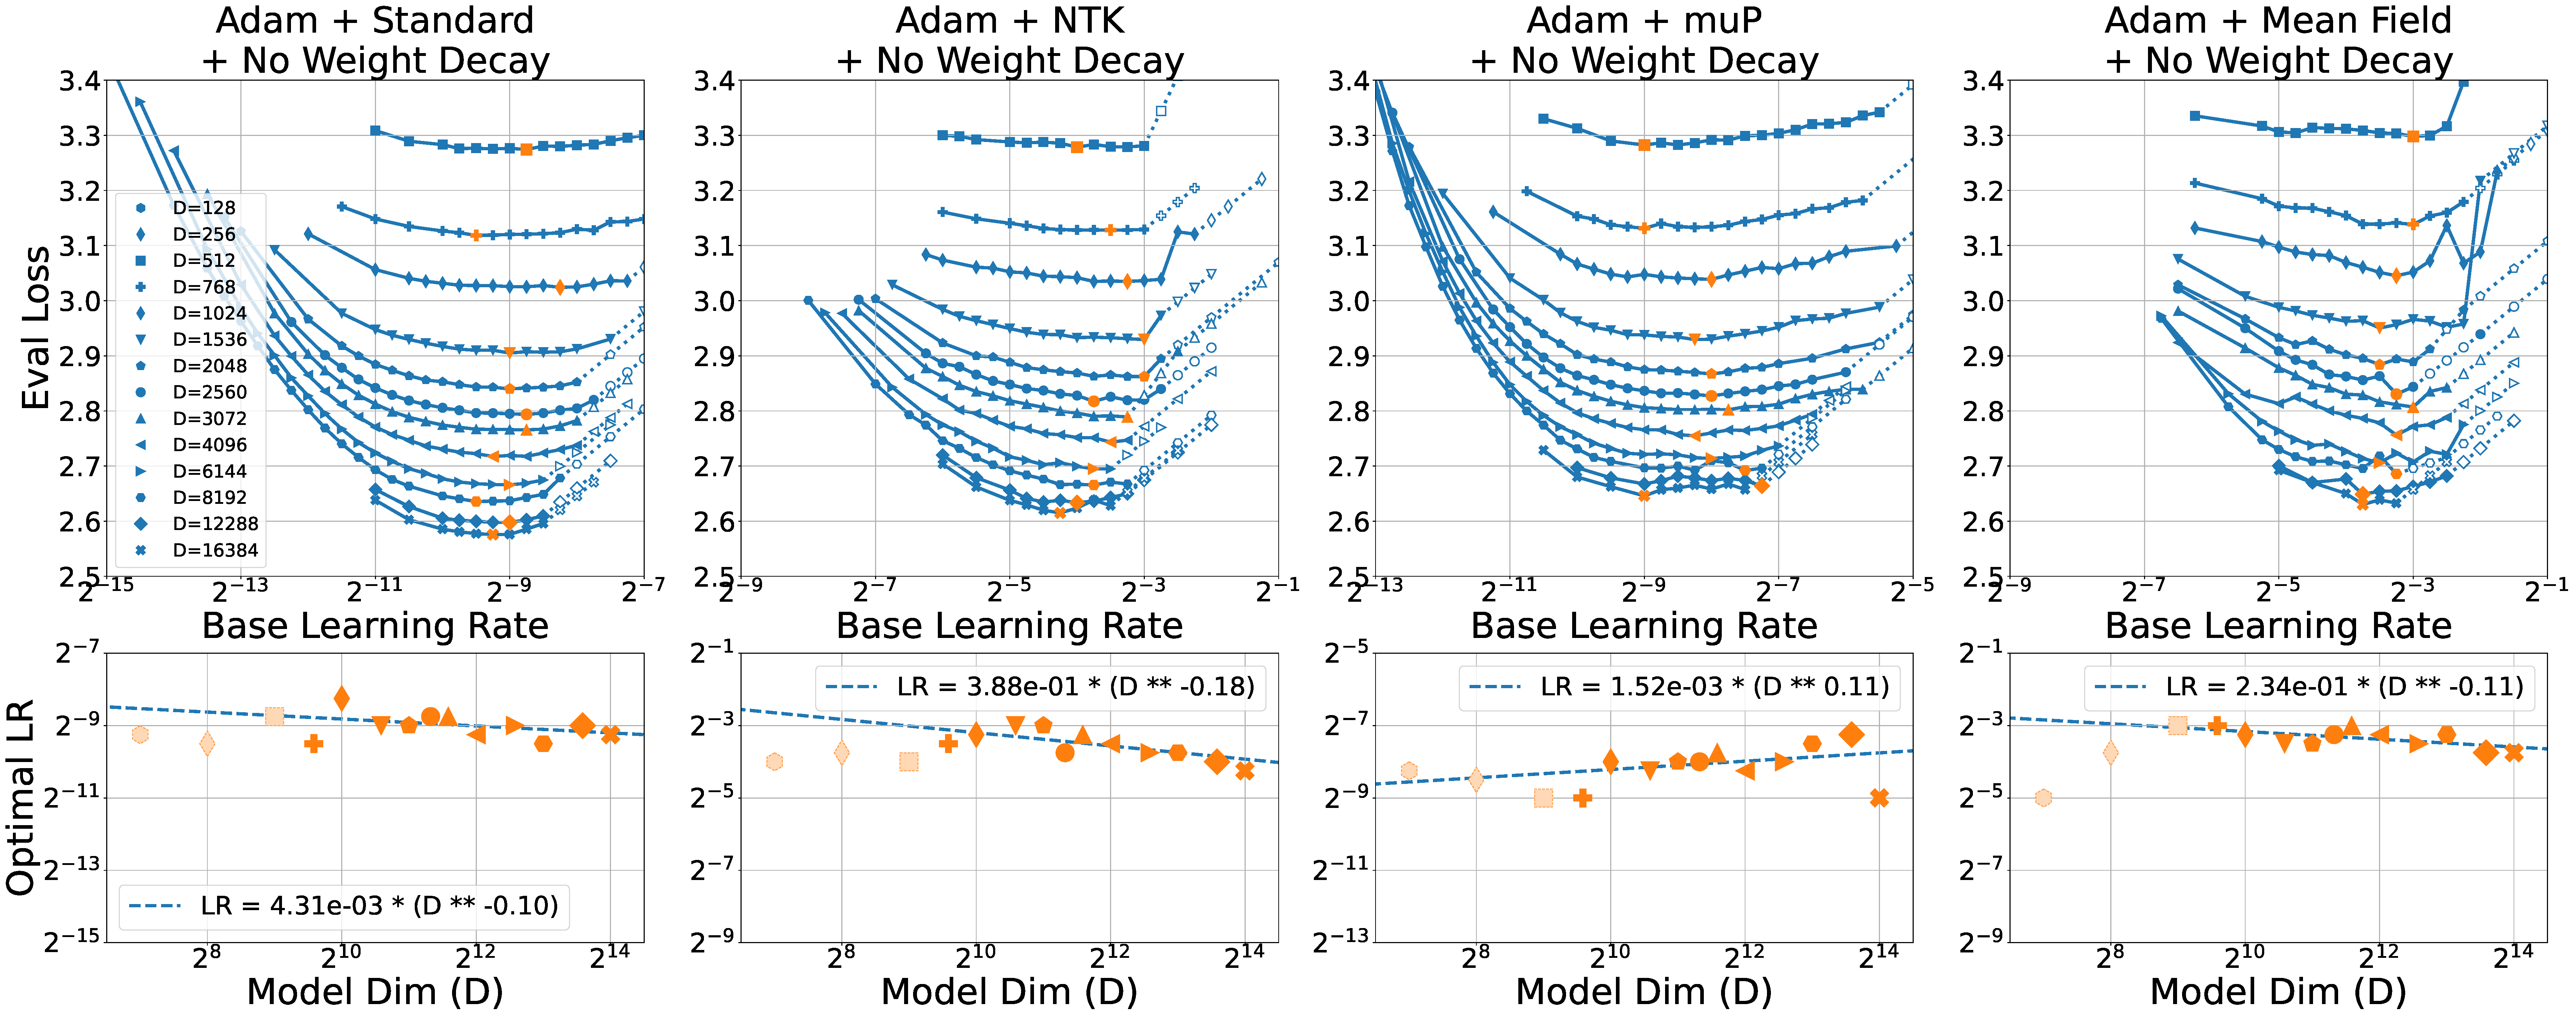
\includegraphics[width=\linewidth]{icml2024/figures/wd_appendix/adam+50k_steps_per_module_lr.pdf}
        
        \figvspace
        
        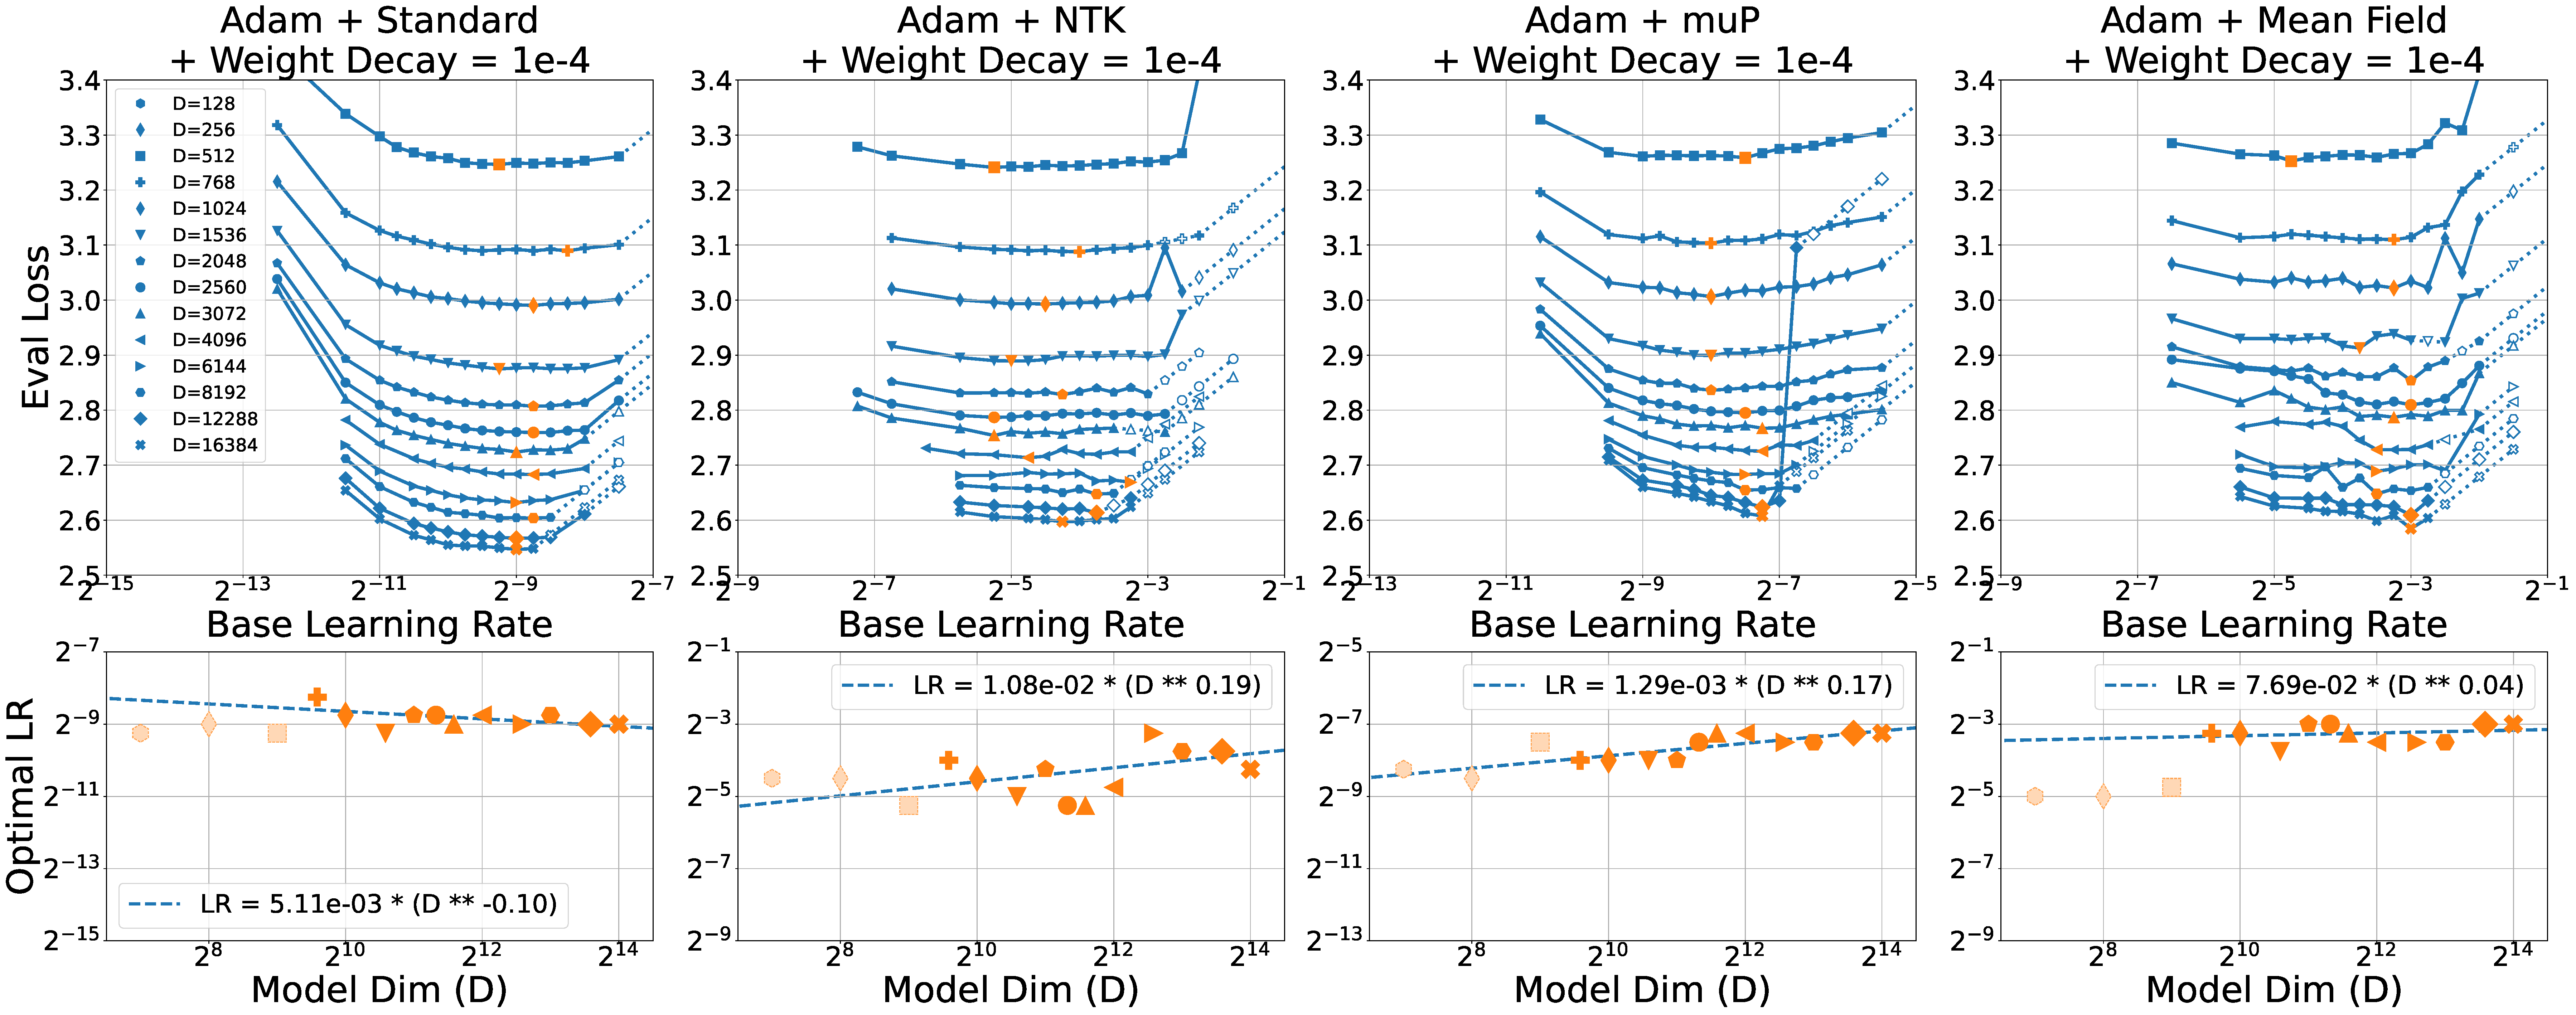
\includegraphics[width=\linewidth]{icml2024/figures/wd_appendix/adam+50k_steps_per_module_lr_wd.pdf}
        \caption{\textbf{Weight decay improves eval losses but learning rate scaling behavior is similar.} Top = Adam + per-layer learning rates assuming full alignment + default constants + no weight decay. Bottom = Adam + per-layer learning rates assuming full alignment + default constants + decoupled weight decay = 1e-4. Number of training steps = $50{,}000$.}
        \label{fig:appendix_adam_weight_decay}
\end{SidewaysFigure}
\clearpage

        
        

\subsection{Adafactor and Adam + Parameter Scaling experiments}
\label{app:adafactor_adam_ps}
As a cross-check that Adafactor and Adam + parameter scaling are in similar width-scaling regimes, we compare the two optimizers on all parameterizations in two settings: global learning rate + default constants and per-layer learning rate + full alignment + optimal constants. Due to the factored matrices in Adafactor, we encountered issues with tensor shape mismatches when using Adafactor with our implementation of FSDP, which the limited the model sizes we could use for Adafactor. Instead, we use Adam + parameter scaling for all our experiments in \cref{sec:results_per_layer}.

See \cref{app:optim_details} for details on the optimizers and hyperparameters. The differences between Adam+parameter scaling and Adafactor are: the factored second moment estimate in Adafactor, different values of beta1 and beta2, update clipping in Adafactor, and the value of epsilon. We see in \cref{fig:adafactor_cross_check} that there are minor differences in performance but overall the optimizers show similar scaling behavior across model sizes up to $4B$ parameters, suggesting these two optimizers should be considered members of the same width-scaling regime.

\vspace{48pt}
\begin{figure*}[ht]
    \begin{center}
        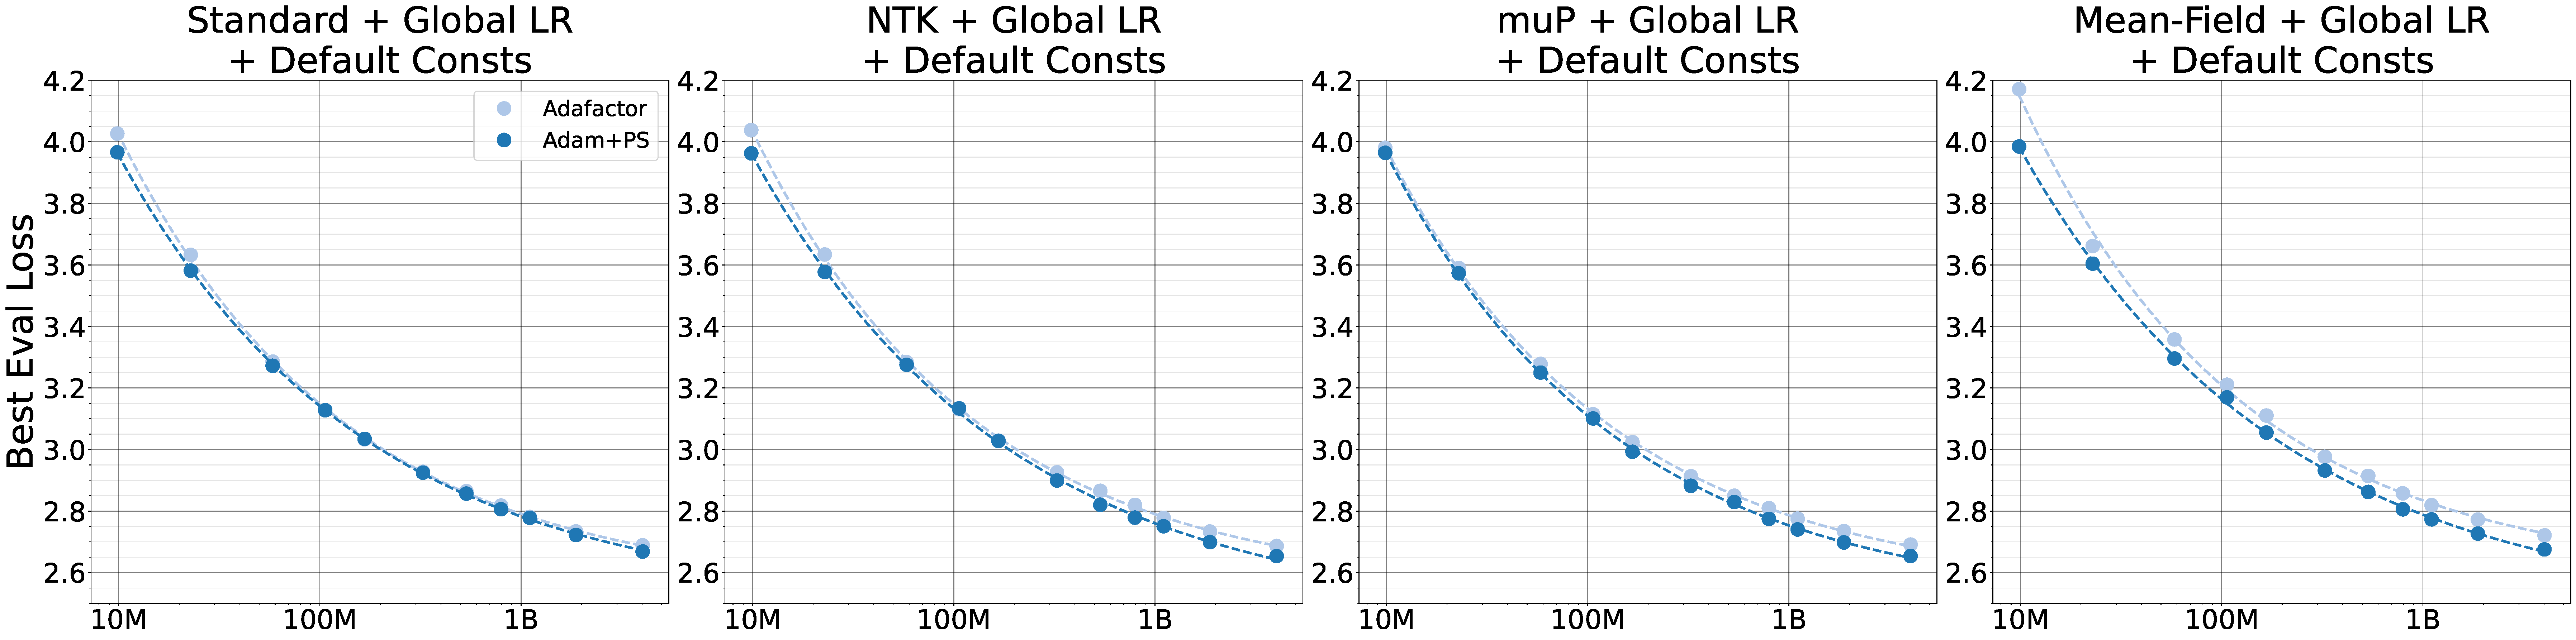
\includegraphics[width=\linewidth, trim={0, 0, 0, 0},clip]{icml2024/figures/adafactor_cross_check/adafactor_cross_check+50k_steps.pdf}
       
        \figvspace

        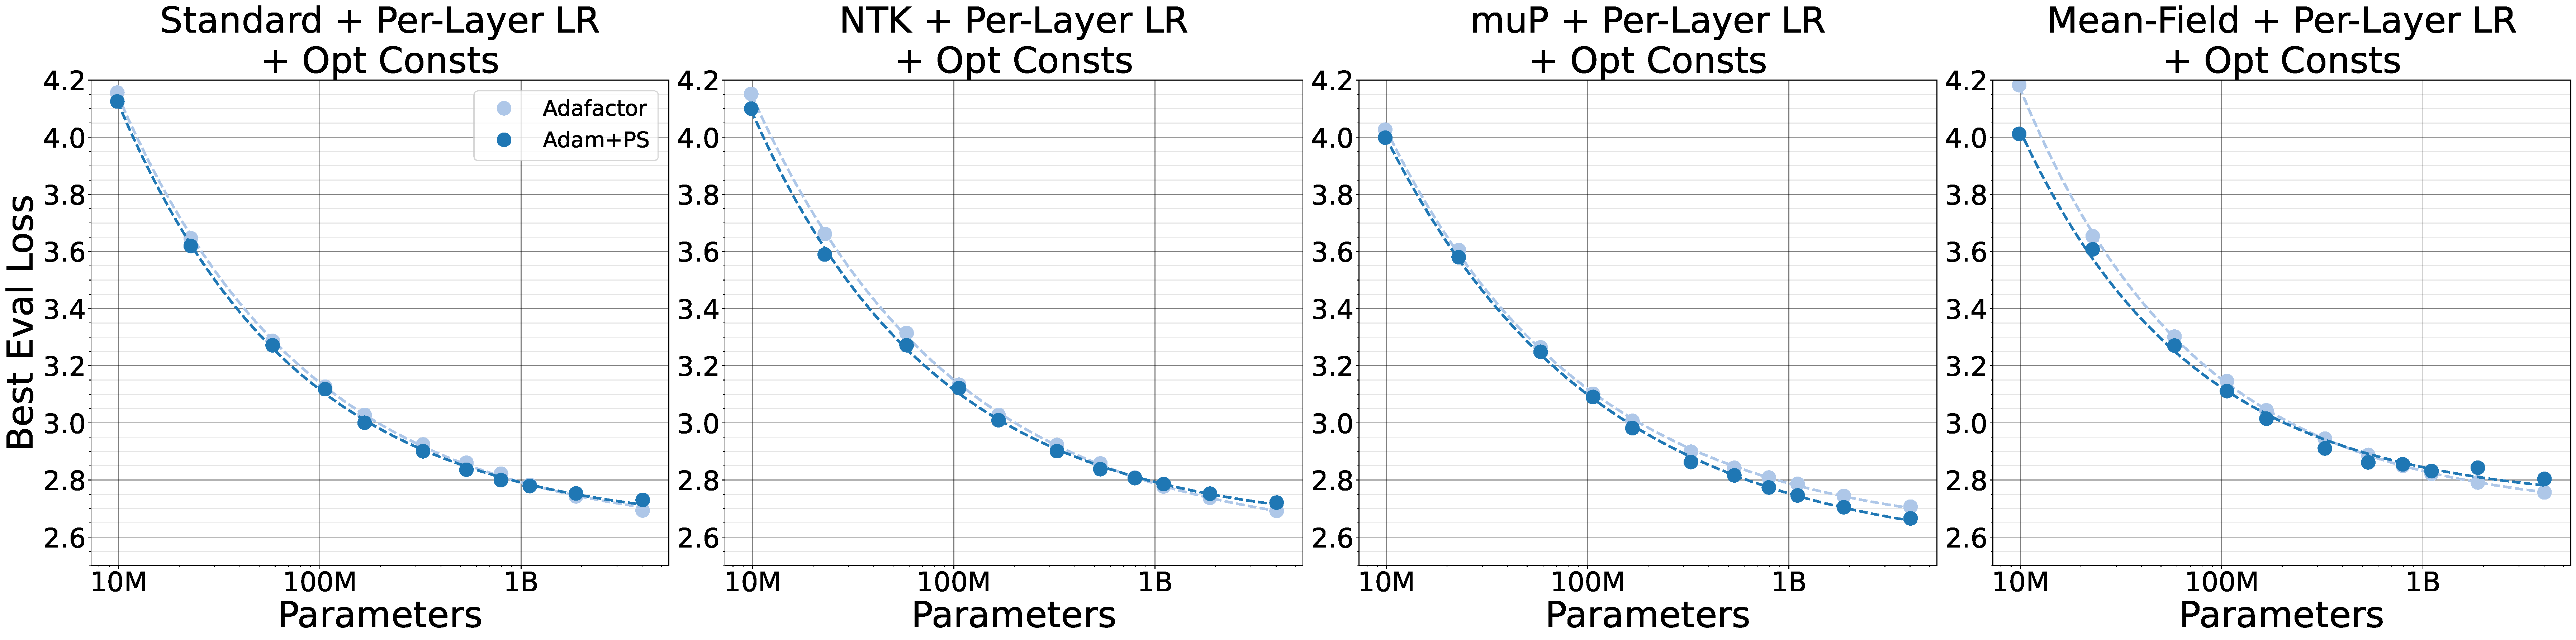
\includegraphics[width=\linewidth, trim={0, 0, 0, 0},clip]{icml2024/figures/adafactor_cross_check/adafactor_cross_check+50k_steps_per_module_lr_optimal_constants.pdf}
        \caption{\centering{\textbf{Adafactor and Adam + parameter scaling are in the same width-scaling regime.} Figures show the best eval loss across a learning rate sweep at each model size for both optimizers. Top row = global learning rate + default constants, bottom row = per-layer learning rate assuming full alignment + optimal constants. There are minor performance differences between the optimizers but the overall scaling behavior is similar in all settings.}}
        \label{fig:adafactor_cross_check}
    \end{center}
\end{figure*}

\clearpage

\subsection{Fixed Step vs Compute Optimal experiments}
\label{app:fixed_vs_compute_opt}
Since the cost of compute is currently the most significant factor that limits the scale of large model training runs, the dominant paradigm for training large models in practice is the compute-optimal regime. The compute-optimal setting~\citep{kaplan2019notes} aims to maximize model performance under a fixed budget of FLOPS for training, where these FLOPS can be traded off between the number of parameters in the model and the number of training tokens the model is trained on. The Chinchilla paper~\citep{hoffmann2022training} finds empirically that the optimal tradeoff occurs when the number of parameters and number of tokens scale in proportion. When the batch size and context length are fixed, as in our setting, the number of training tokens is proportional to the number of training steps. Due to the $n \times n$ parameter matrices in dense hidden layers with width $n$, the number of parameters grow quadratically with respect to the width. Therefore, the Chinchilla results imply that the compute optimal number of steps grows \emph{quadratically} with respect to the model width.

This contradicts the fixed step assumption used in the theoretical derivations in both this paper and \citet{yang2021tensoriv,yang2023tensorivb}, which assume that the number of training steps $T$ is $O(1)$. Intuitively, this fixed step assumption is used so that the derivations can consider the contributions to the scaling exponents of a single step at a time: if we satisfactorily bound the contribution of each step to the scaling exponents, and then take only a constant number of steps, then the constant number of steps does not introduce any width-dependent scaling factors. The naive extension of this theory to a setting with $\Theta(n^2)$ instead of $O(1)$ training steps would give impractical bounds: in the worst-case analysis, each learning rate would need to be divided by $n^2$ to correct for the $n^2$ number of steps giving learning rates that are far too conservative to be useful.

We therefore take an empirical approach rather than a worst-case theoretical analysis to investigate the role of the training horizon. We perform a set of experiments using both fixed step and compute optimal training horizons in the global learning rate settings for SGD+momentum, Adam and Adafactor across all parameterizations using default constant learning rate multipliers. In each setting, we sweep both model width and learning rate, and then fit a power law with an irreducible loss term to determine the scaling exponent for the optimal learning rate. The measured learning rate exponents are reported in \cref{tab:compute_opt_exponents}. For all fixed step experiments, we train for $50{,}000$ steps. For the compute optimal setting, we compute the training horizon using the Chinchilla-optimal heuristic \citep{hoffmann2022training} with 20x multiplier, i.e. the number of training tokens is equal to 20 times the number of non-embedding parameters. Full results for the learning rate sweeps are included in \cref{fig:app_compute_opt_sgd}, \ref{fig:app_compute_opt_adam} and \ref{fig:app_compute_opt_adafactor}.

\begin{table}[htbp]
  \centering
  \caption{\textbf{Power law exponents fit to the optimal learning rate vs model dimension} for each optimizer $\times$ parameterization combination, measured for fixed step (50k) and compute optimal training horizon experiments.}
  \vspace{2pt}
  \begin{adjustbox}{scale=0.8}
    \begin{tabular}{rrrr}
        \toprule
            &           & \textbf{Fixed Step (50k)}           & \textbf{Compute Optimal}  \\
         \midrule
          \multirow{4}{*}{SGD} & STP        & -0.38         & -1.27  \\
          & NTK                             & 0.56          & 0.04   \\
          & muP                             & -0.17         & -0.85  \\
          & MFP	                            & 0.31          & -0.41  \\  \midrule
          \multirow{4}{*}{Adam} & STP       & -0.95         & -1.18  \\
          & NTK	                            & -0.66	        & -0.67  \\
          & muP	                            & -1.09         & -1.38  \\
          & MFP	                            & -0.16         & -0.45  \\ \midrule
          \multirow{4}{*}{Adafactor} & STP  & -0.12         & -0.55  \\
          & NTK                             & -0.10         & -0.52  \\
          & muP                             & -0.15         & -0.66  \\
          & MFP                             & -0.09         & -0.57 \\
        \bottomrule
    \end{tabular}
    \end{adjustbox}
  \label{tab:compute_opt_exponents}
\end{table}

Our exponent measurements show that in every parameterization $\times$ optimizer setting, the learning rate exponent in the compute optimal setting is \emph{smaller} than in the fixed steps setting, indicating that the learning rate would need to decrease more aggressively as width grows than predictions from the fixed steps setting would imply. The median difference from the twelve optimizer $\times$ parameterization settings is $0.46$ and ranges from $0.01$ to $0.89$. We note this difference of $0.46$ is much less than the difference of $2$ that would come from the naive worst-case theoretical analysis.

This result has implications both for theoretical and empirical settings. First, it motivates theoretical work to consider the compute optimal setting instead of the fixed steps setting. Second, it implies that hyperparameter search should be careful not to assume that results from the fixed step setting will extrapolate to the compute optimal setting. In particular, given a fixed compute budget to spend on hyperparameter search before training a single large model with a compute optimal horizon, one possible approach to choosing the learning rate would be to train model sizes close to the final model size for shorter training horizons, and use this to extrapolate the best learning rate for the large model compute optimal run. A priori, this strategy might be advantageous because the shorter training horizons let you use larger models for the same hyperparameter search budget so the search occurs closer in size to the final model. However, our results suggest that this may not be a viable strategy: if we extrapolate a learning rate to larger models based on an exponent fitted in the fixed steps setting, we may significantly overestimate the learning rate that is optimal in the compute optimal setting. Instead, we recommend considering performing the hyperparameter search for the learning rate by training smaller models at their compute optimal training horizon and then extrapolating across model sizes to the compute optimal setting for the largest model.

\clearpage
\thispagestyle{plain}
\begin{SidewaysFigure}
\centering{\textbf{SGD global learning rate experiments: 50k steps and compute optimal}}\\
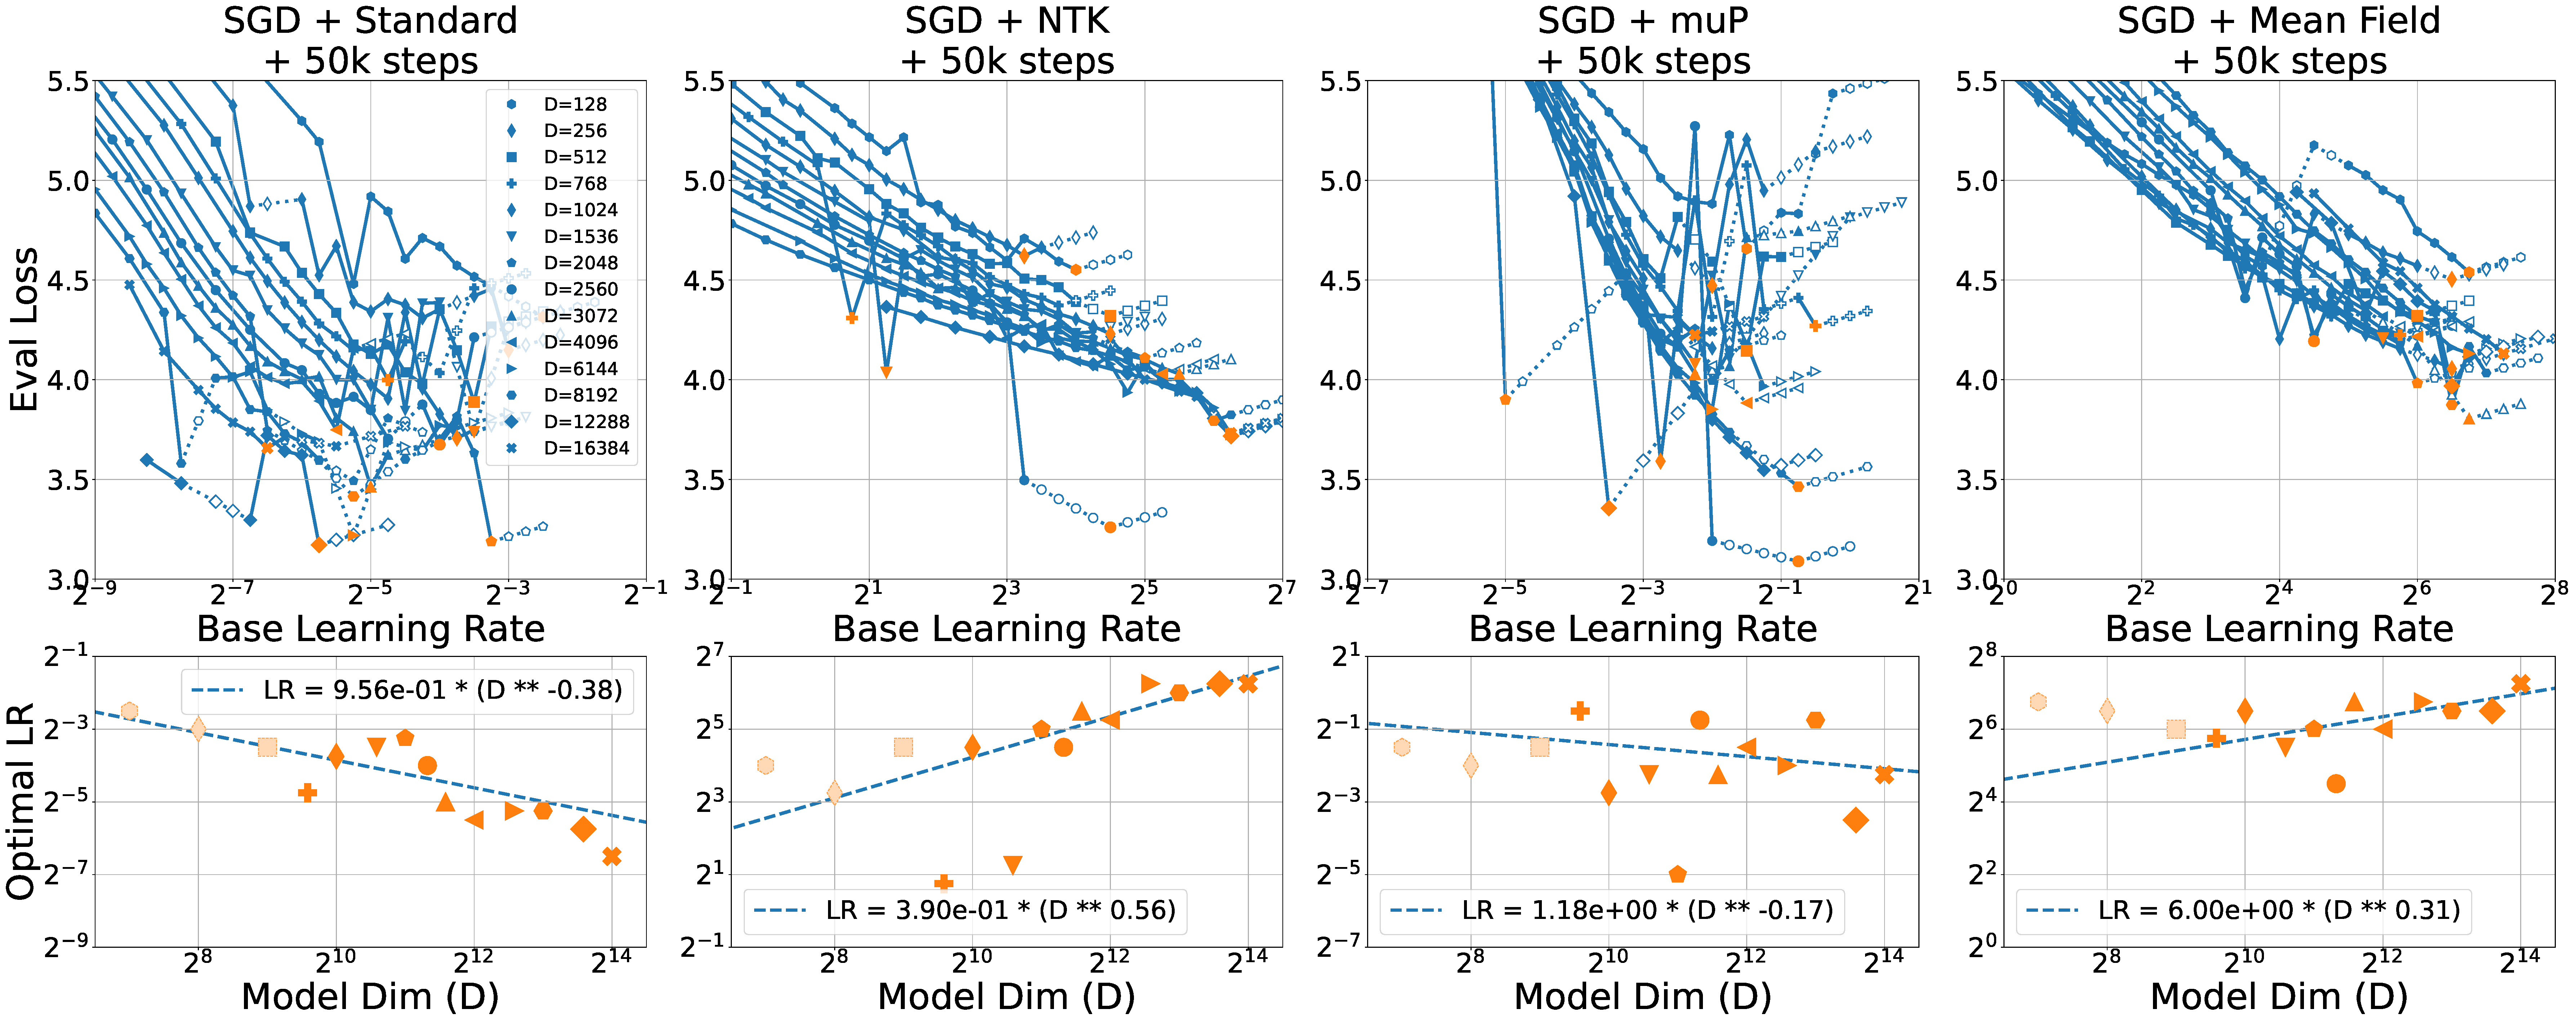
\includegraphics[width=0.98\linewidth]{icml2024/figures/lr_sweeps/compute_opt_appendix/sgd+50k_steps.pdf}

\figvspace

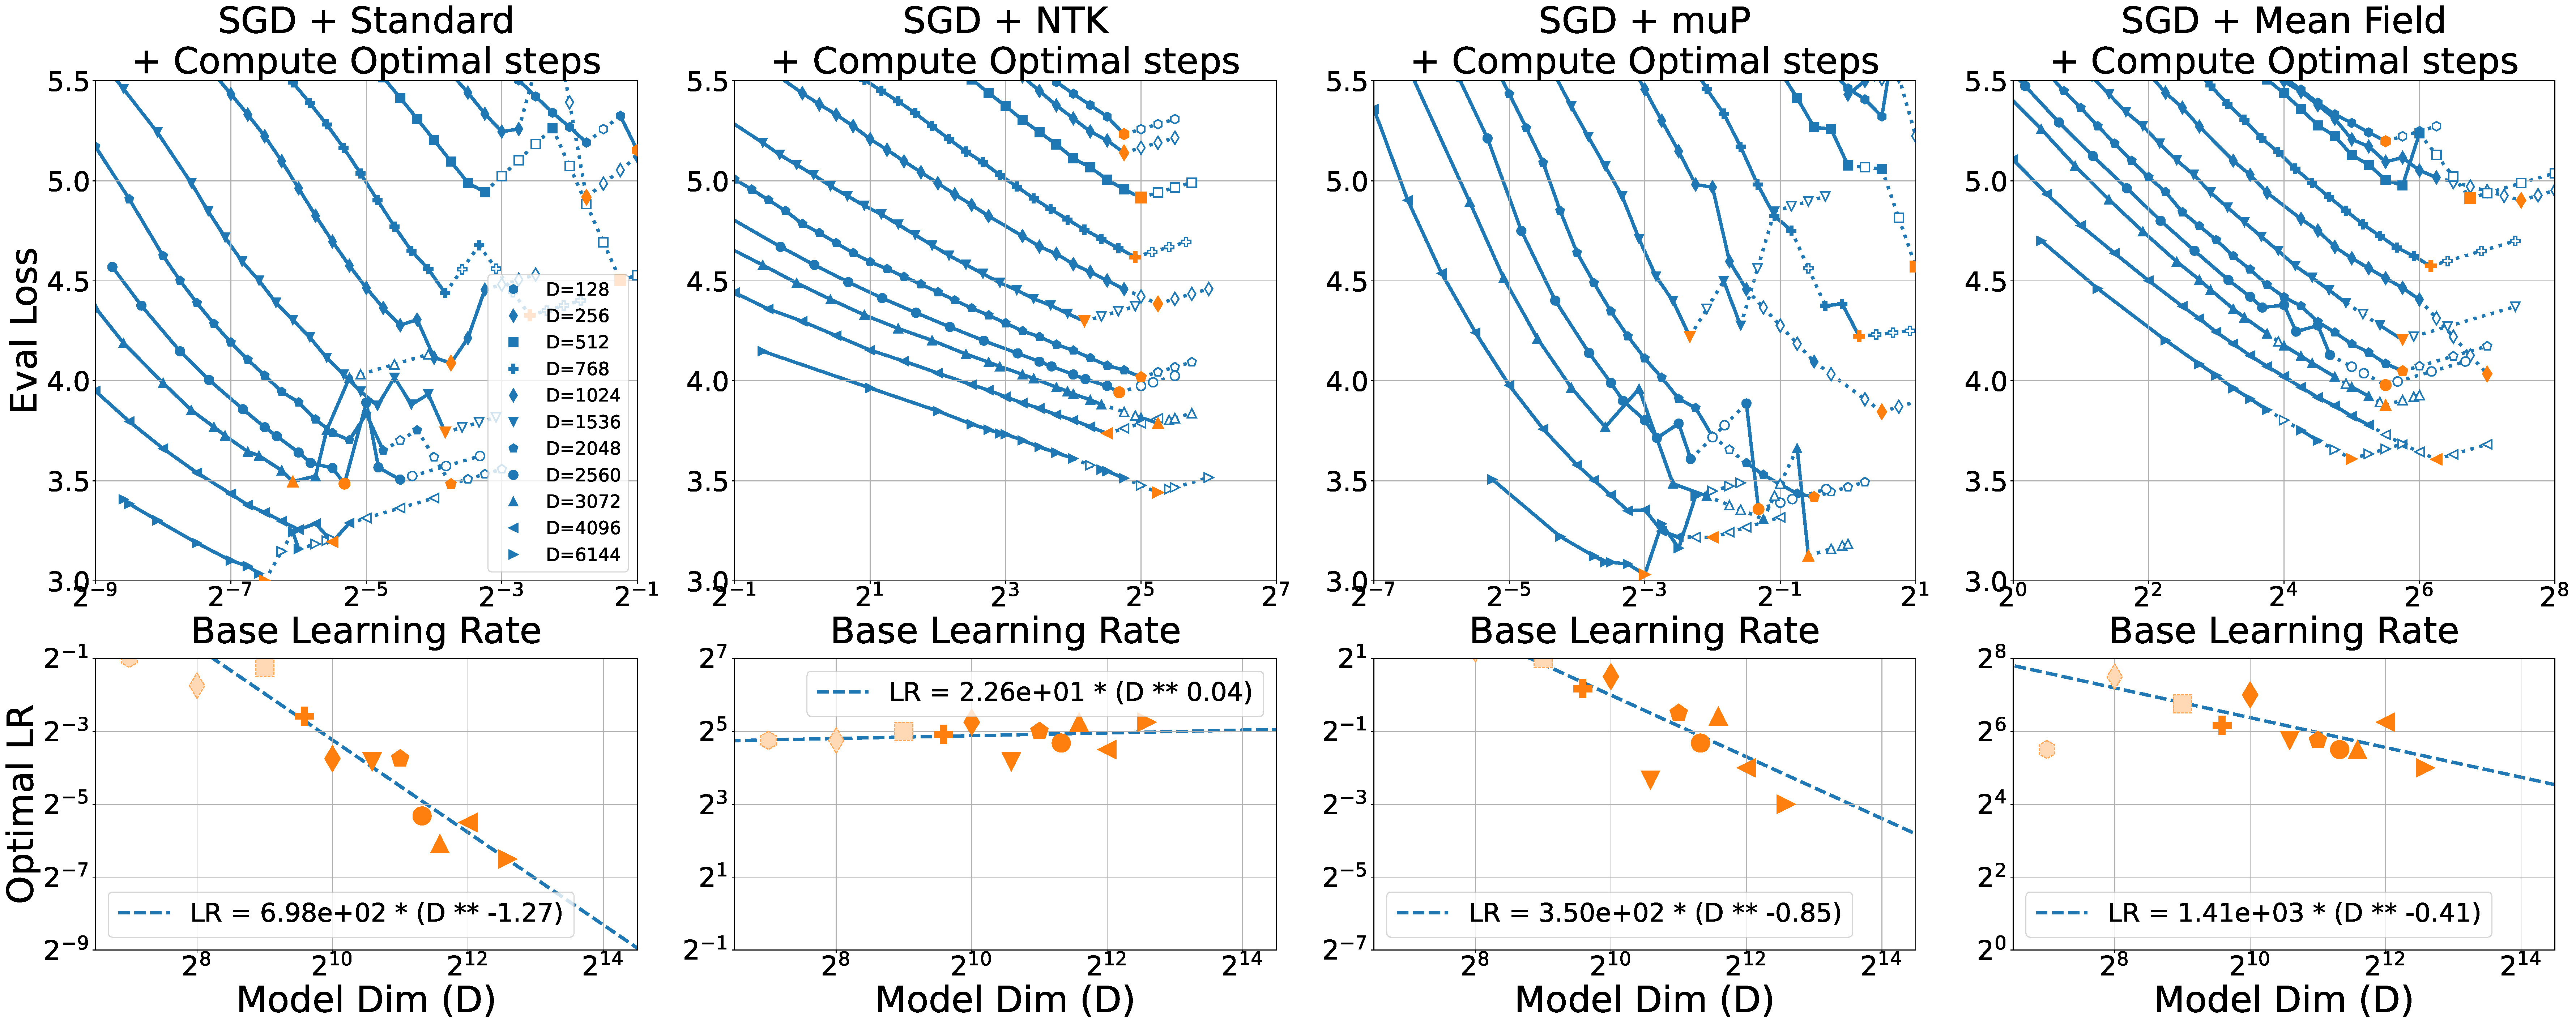
\includegraphics[width=0.98\linewidth]{icml2024/figures/lr_sweeps/compute_opt_appendix/sgd+compute_opt.pdf}
\caption{SGD learning rate sweeps and power laws fit to optimal learning rate vs model dim, using global learning rate and default constants. Top = $50{,}000$ steps. Bottom = compute optimal (Chinchilla 20x) training steps.}
\label{fig:app_compute_opt_sgd}
\end{SidewaysFigure}
\clearpage

\thispagestyle{plain}
\begin{SidewaysFigure}
\centering{\textbf{Adam global learning rate experiments: 50k steps and compute optimal}}\\
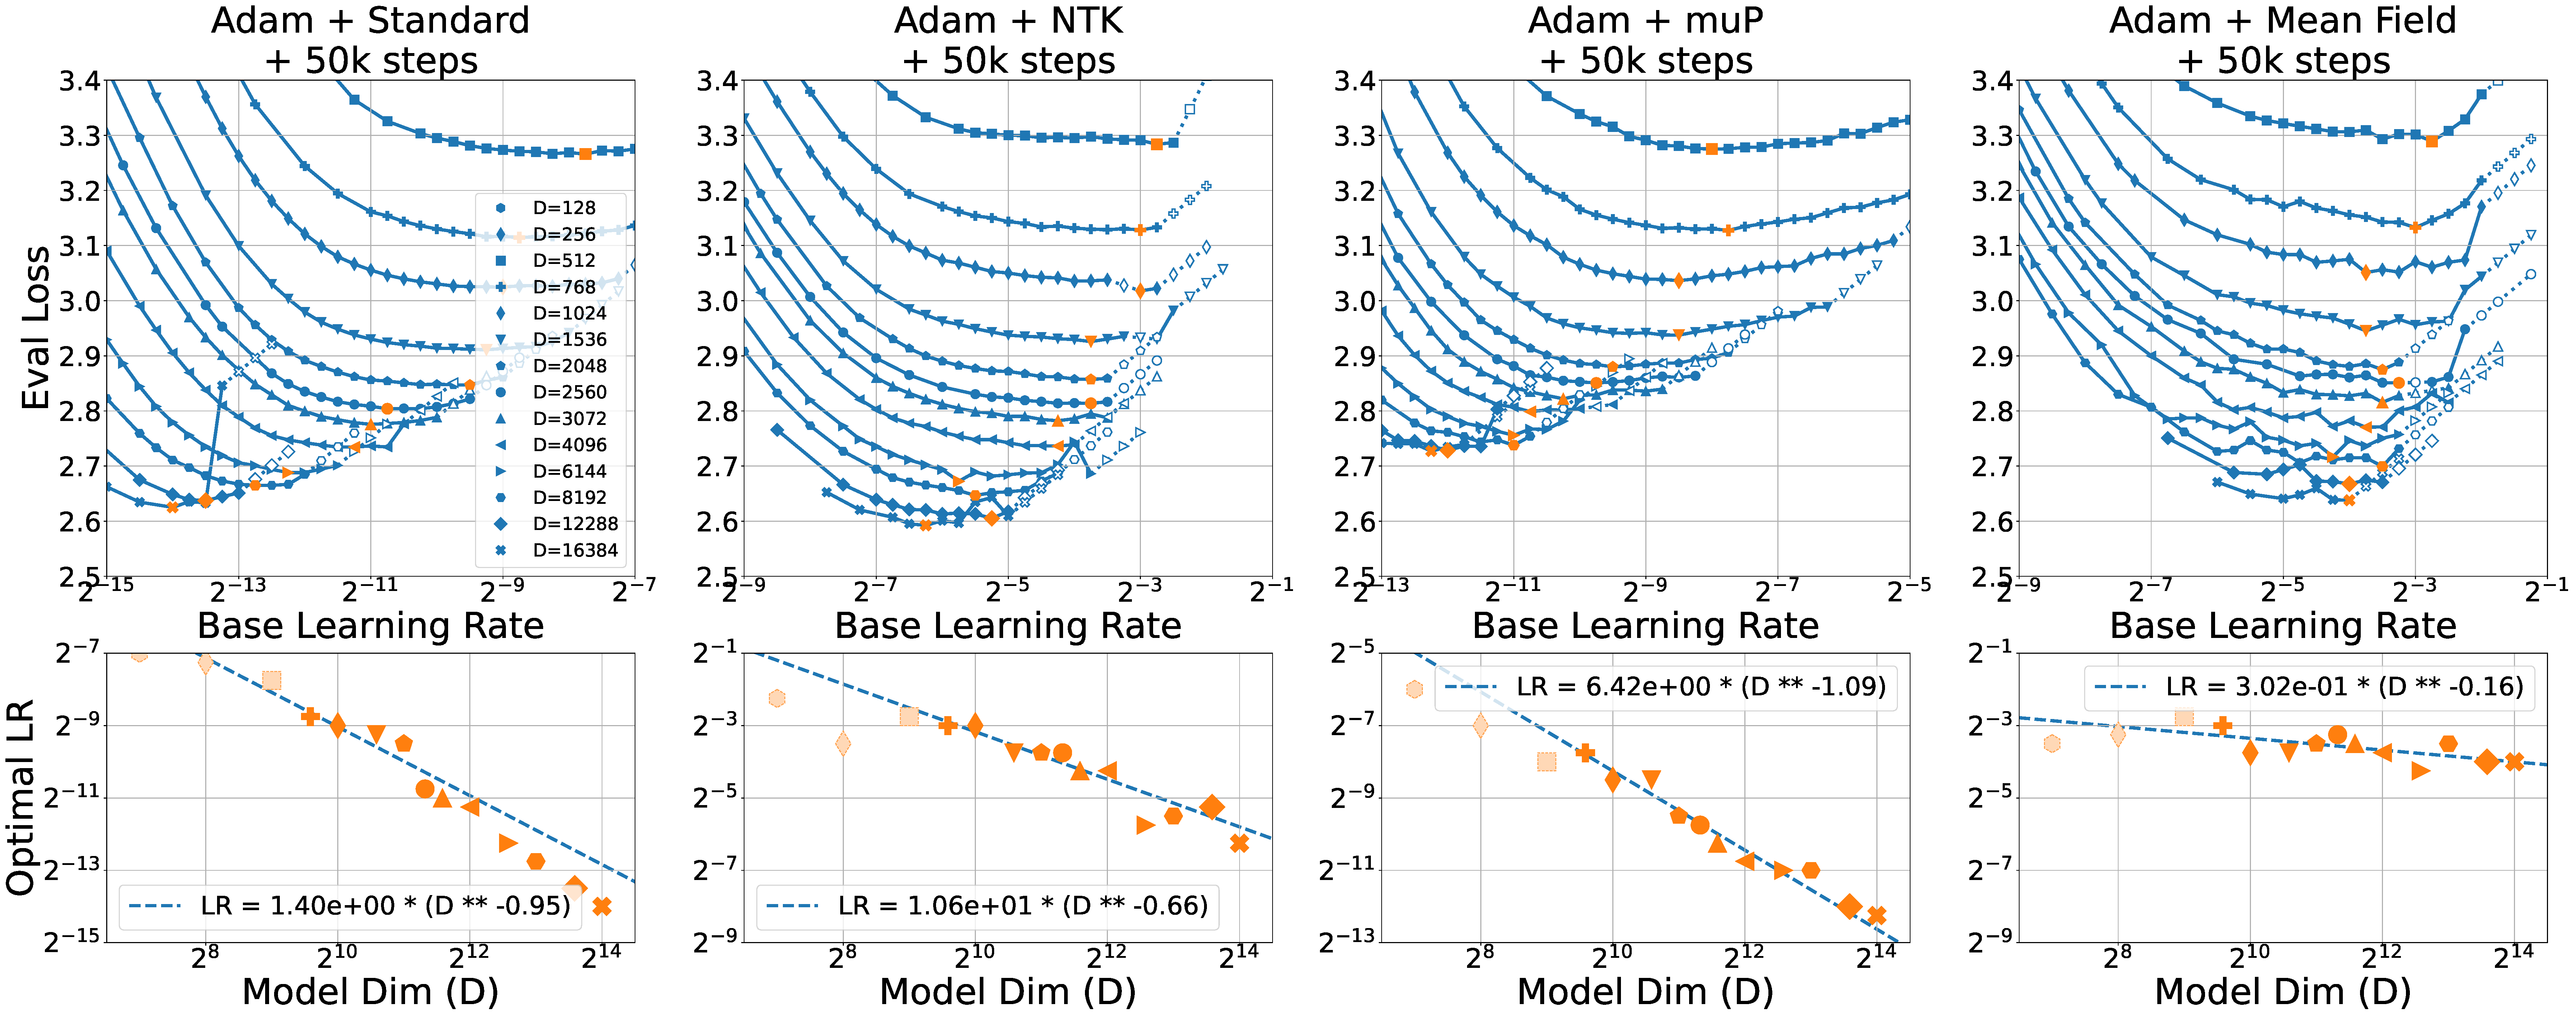
\includegraphics[width=0.98\linewidth]{icml2024/figures/lr_sweeps/compute_opt_appendix/adam+50k_steps.pdf}

\figvspace

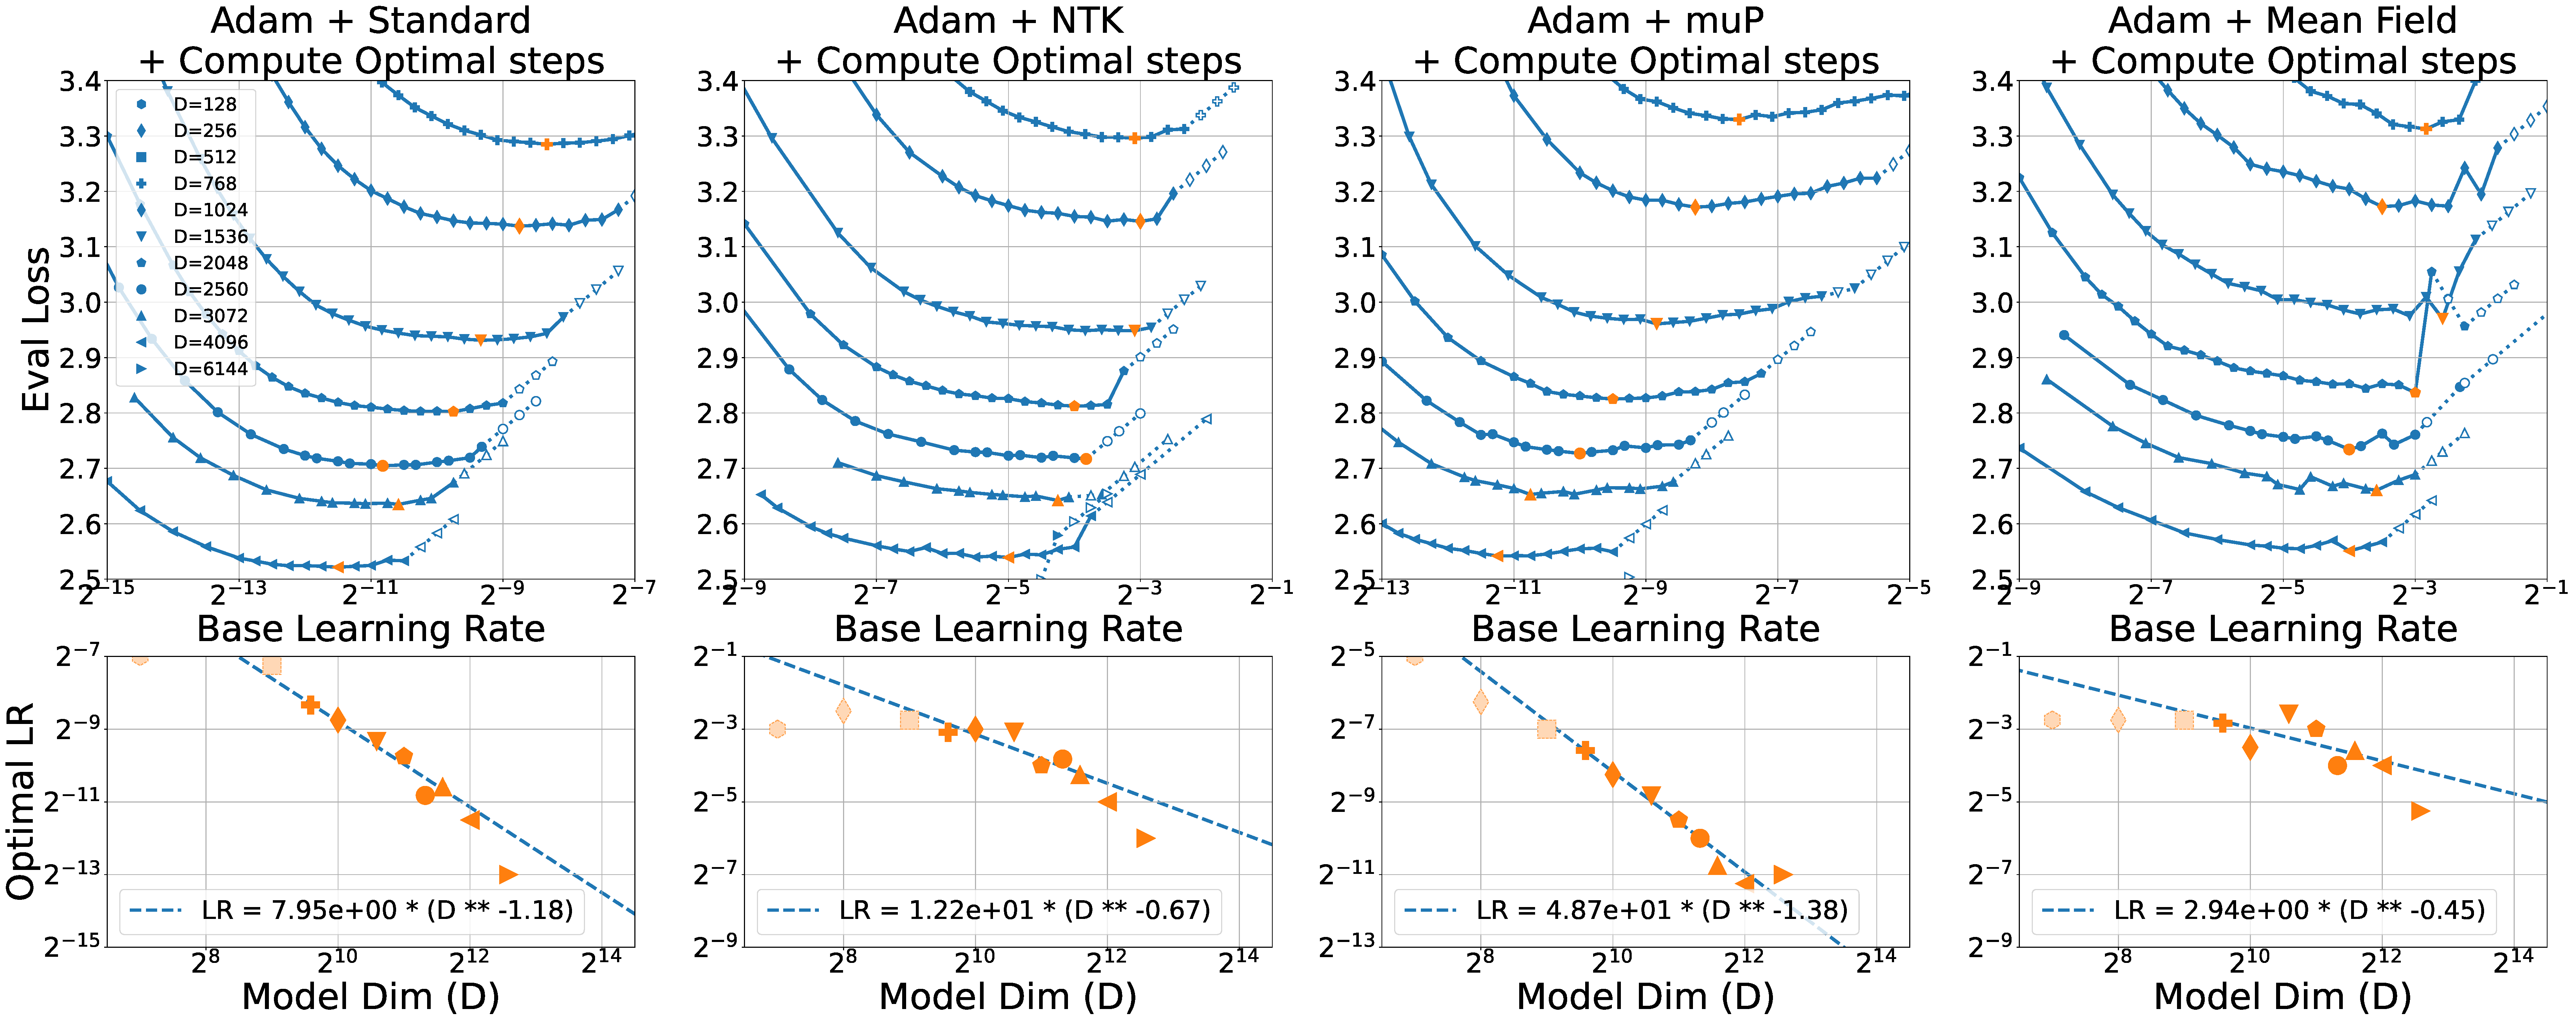
\includegraphics[width=0.98\linewidth]{icml2024/figures/lr_sweeps/compute_opt_appendix/adam+compute_opt.pdf}
\caption{Adam learning rate sweeps and power laws fit to optimal learning rate vs model dim, using global learning rate and default constants. Top = $50{,}000$ steps. Bottom = compute optimal (Chinchilla 20x) training steps.}
\label{fig:app_compute_opt_adam}
\end{SidewaysFigure}
\clearpage

\thispagestyle{plain}
\begin{SidewaysFigure}
\centering{\textbf{Adafactor global learning rate experiments: 50k steps and compute optimal}}\\
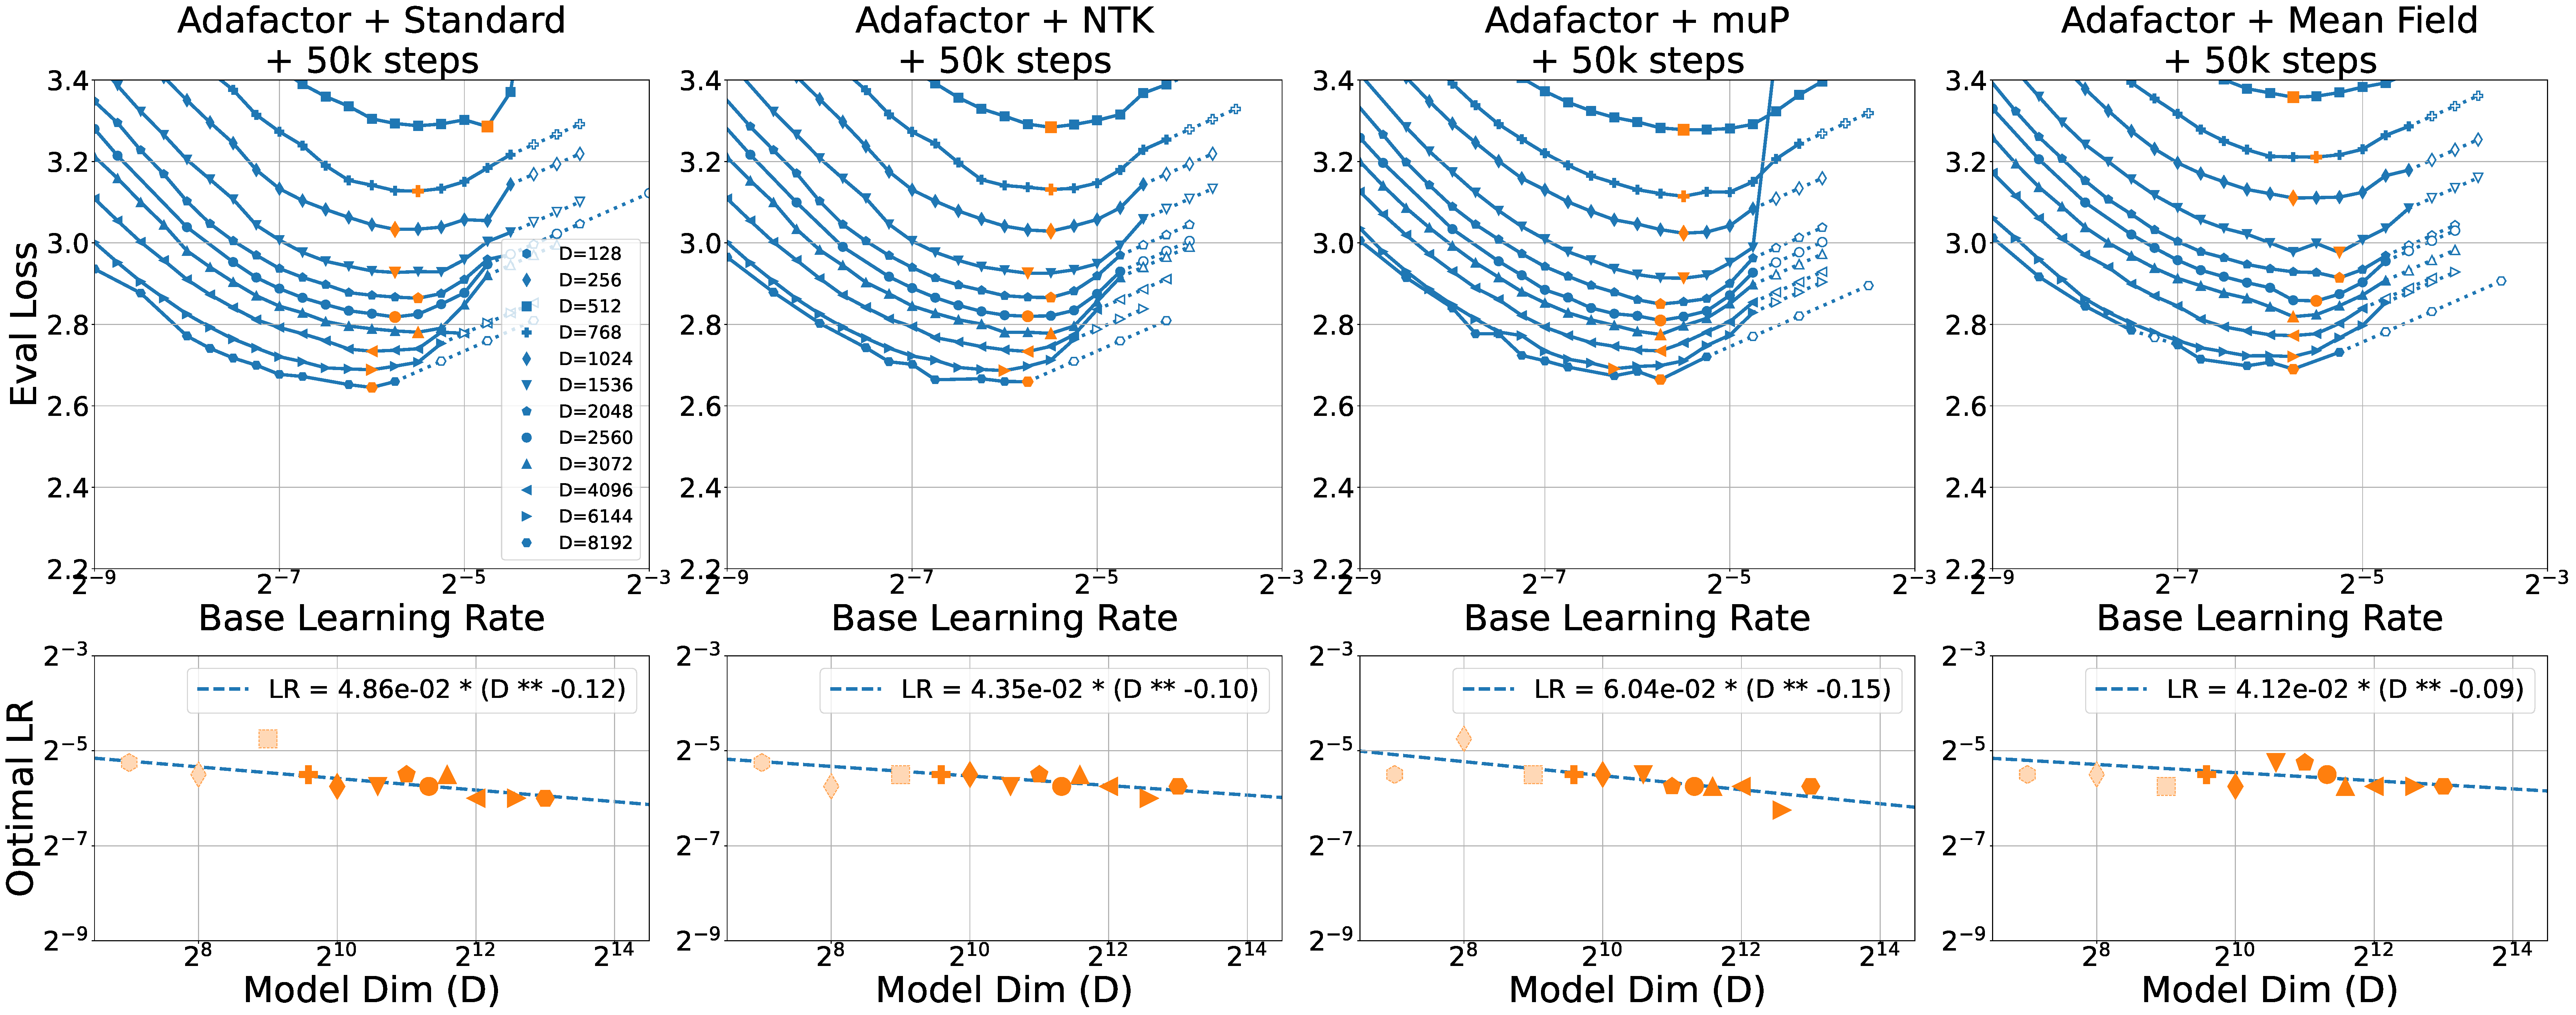
\includegraphics[width=0.98\linewidth]{icml2024/figures/lr_sweeps/compute_opt_appendix/adafactor+50k_steps.pdf}

\figvspace

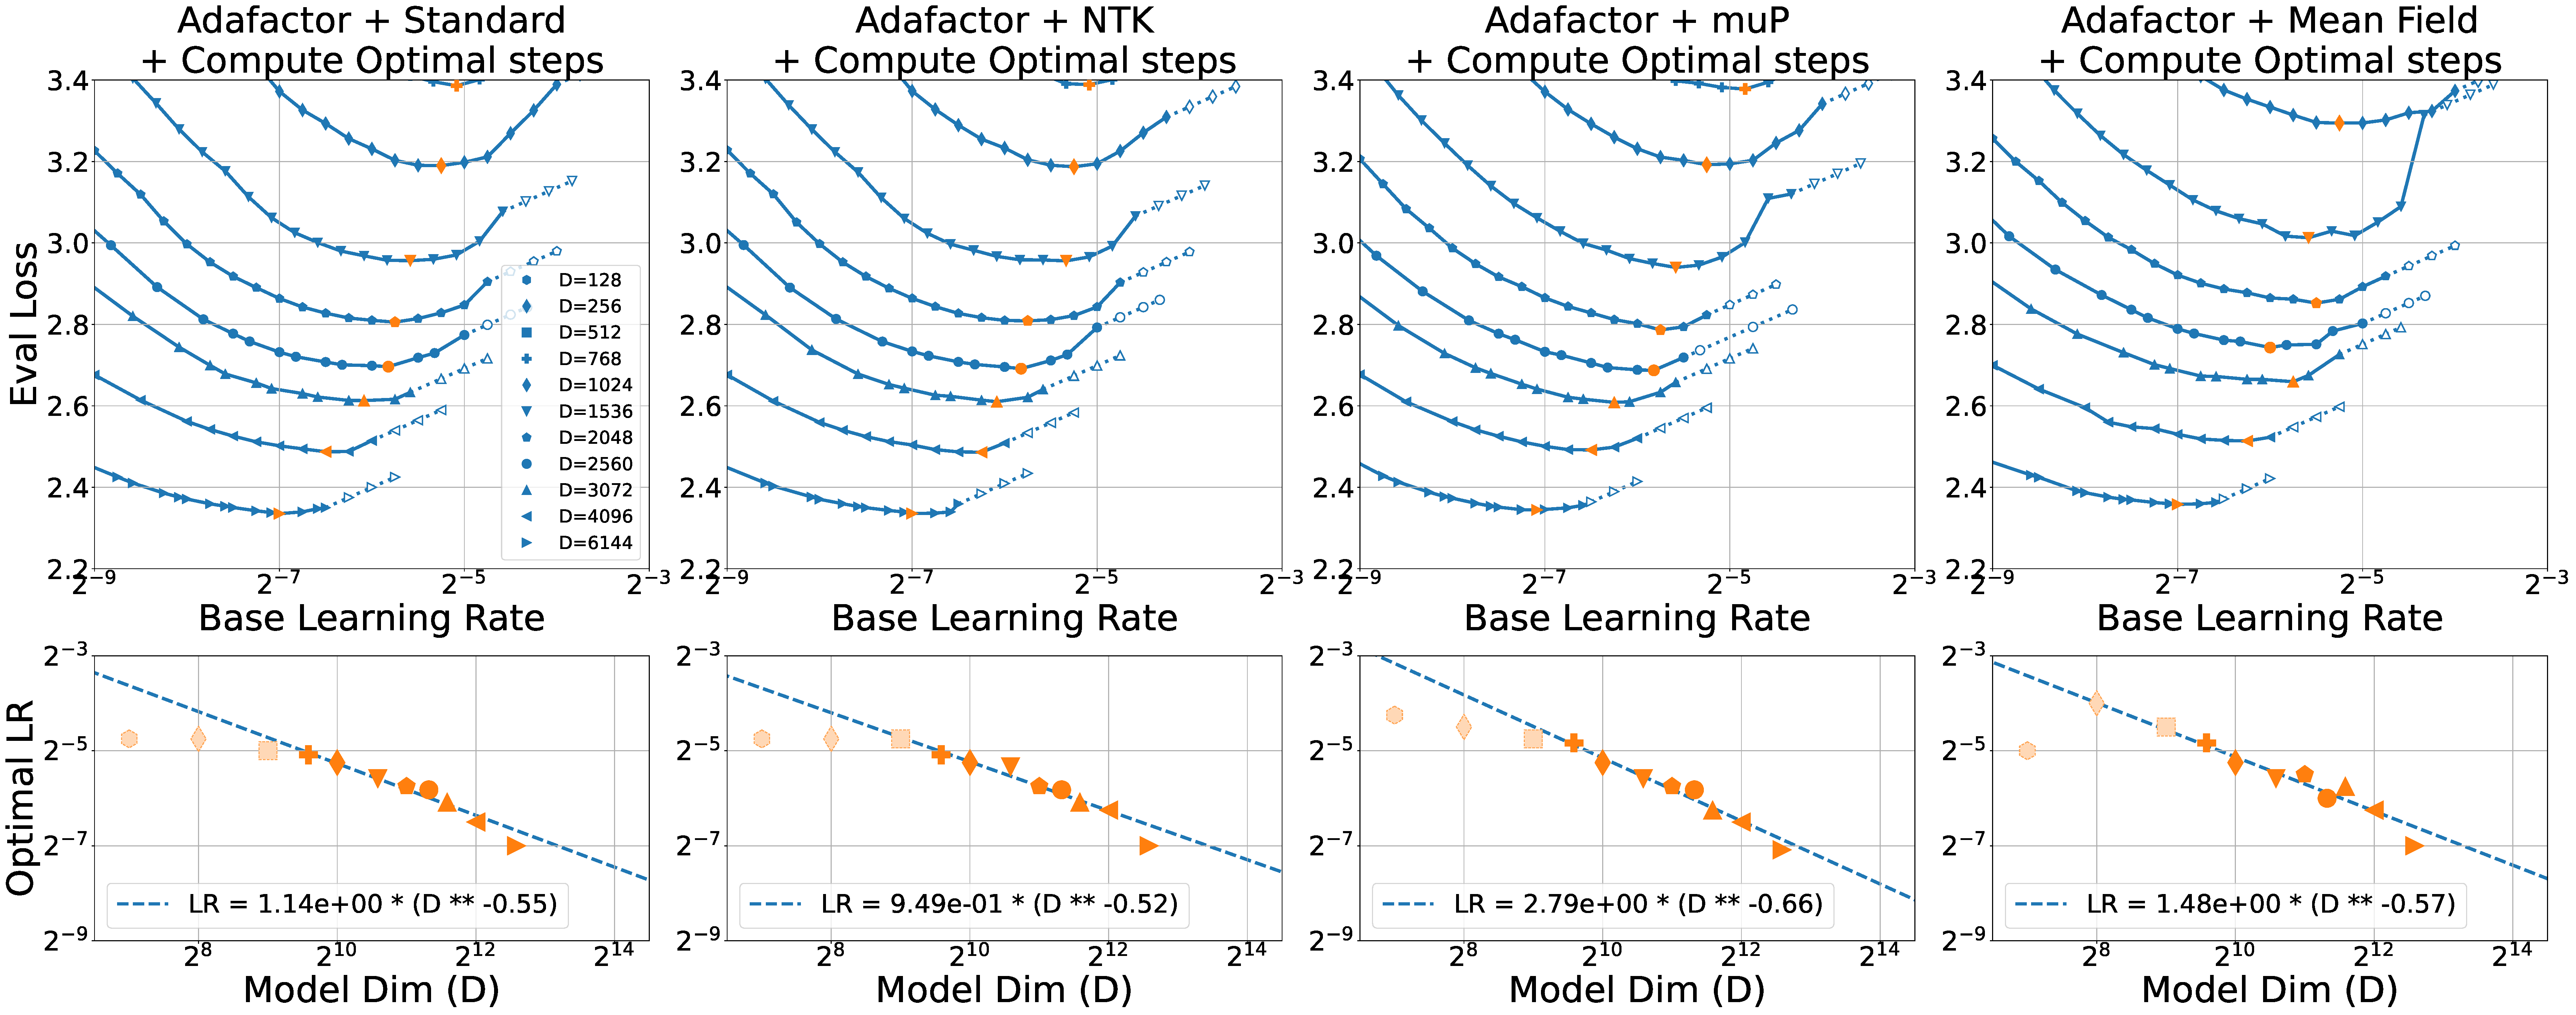
\includegraphics[width=0.98\linewidth]{icml2024/figures/lr_sweeps/compute_opt_appendix/adafactor+compute_opt.pdf}
\caption{Adafactor learning rate sweeps and power laws fit to optimal learning rate vs model dim, using global learning rate and default constants. Top = $50{,}000$ steps. Bottom = compute optimal (Chinchilla 20x) training steps.}
\label{fig:app_compute_opt_adafactor}
\end{SidewaysFigure}
\clearpage




\clearpage
\thispagestyle{plain}
\begin{SidewaysFigure}
\subsection{Learning Rate Sweeps for SGD, all settings}
\label{sec:app_lr_sweeps_sgd}
\vspace{12pt}
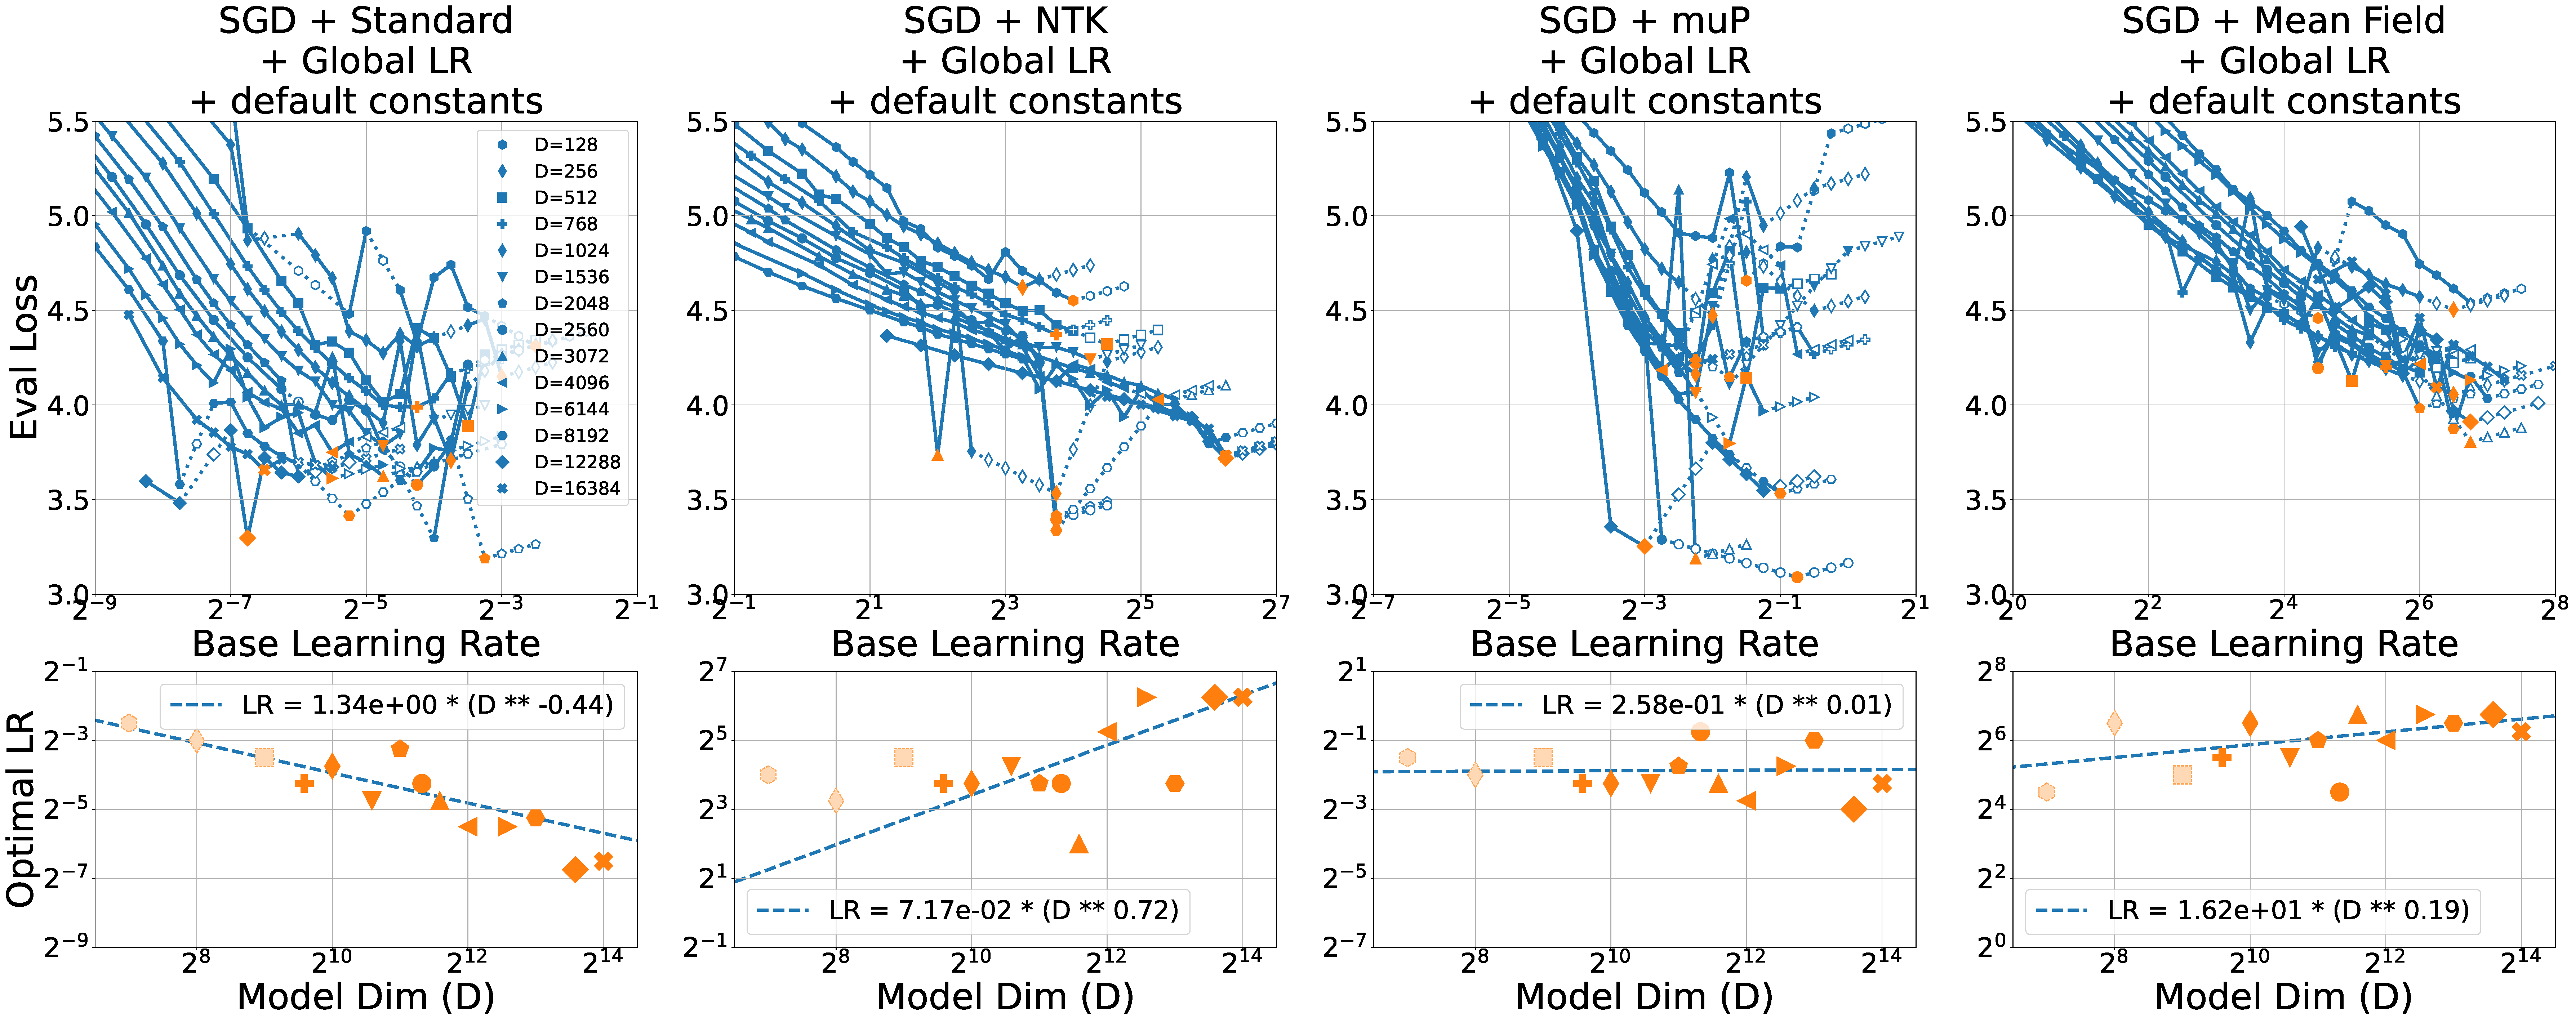
\includegraphics[width=0.98\linewidth]{icml2024/figures/lr_sweeps/appendix/sgd/sgd+50k_steps.pdf}

\figvspace

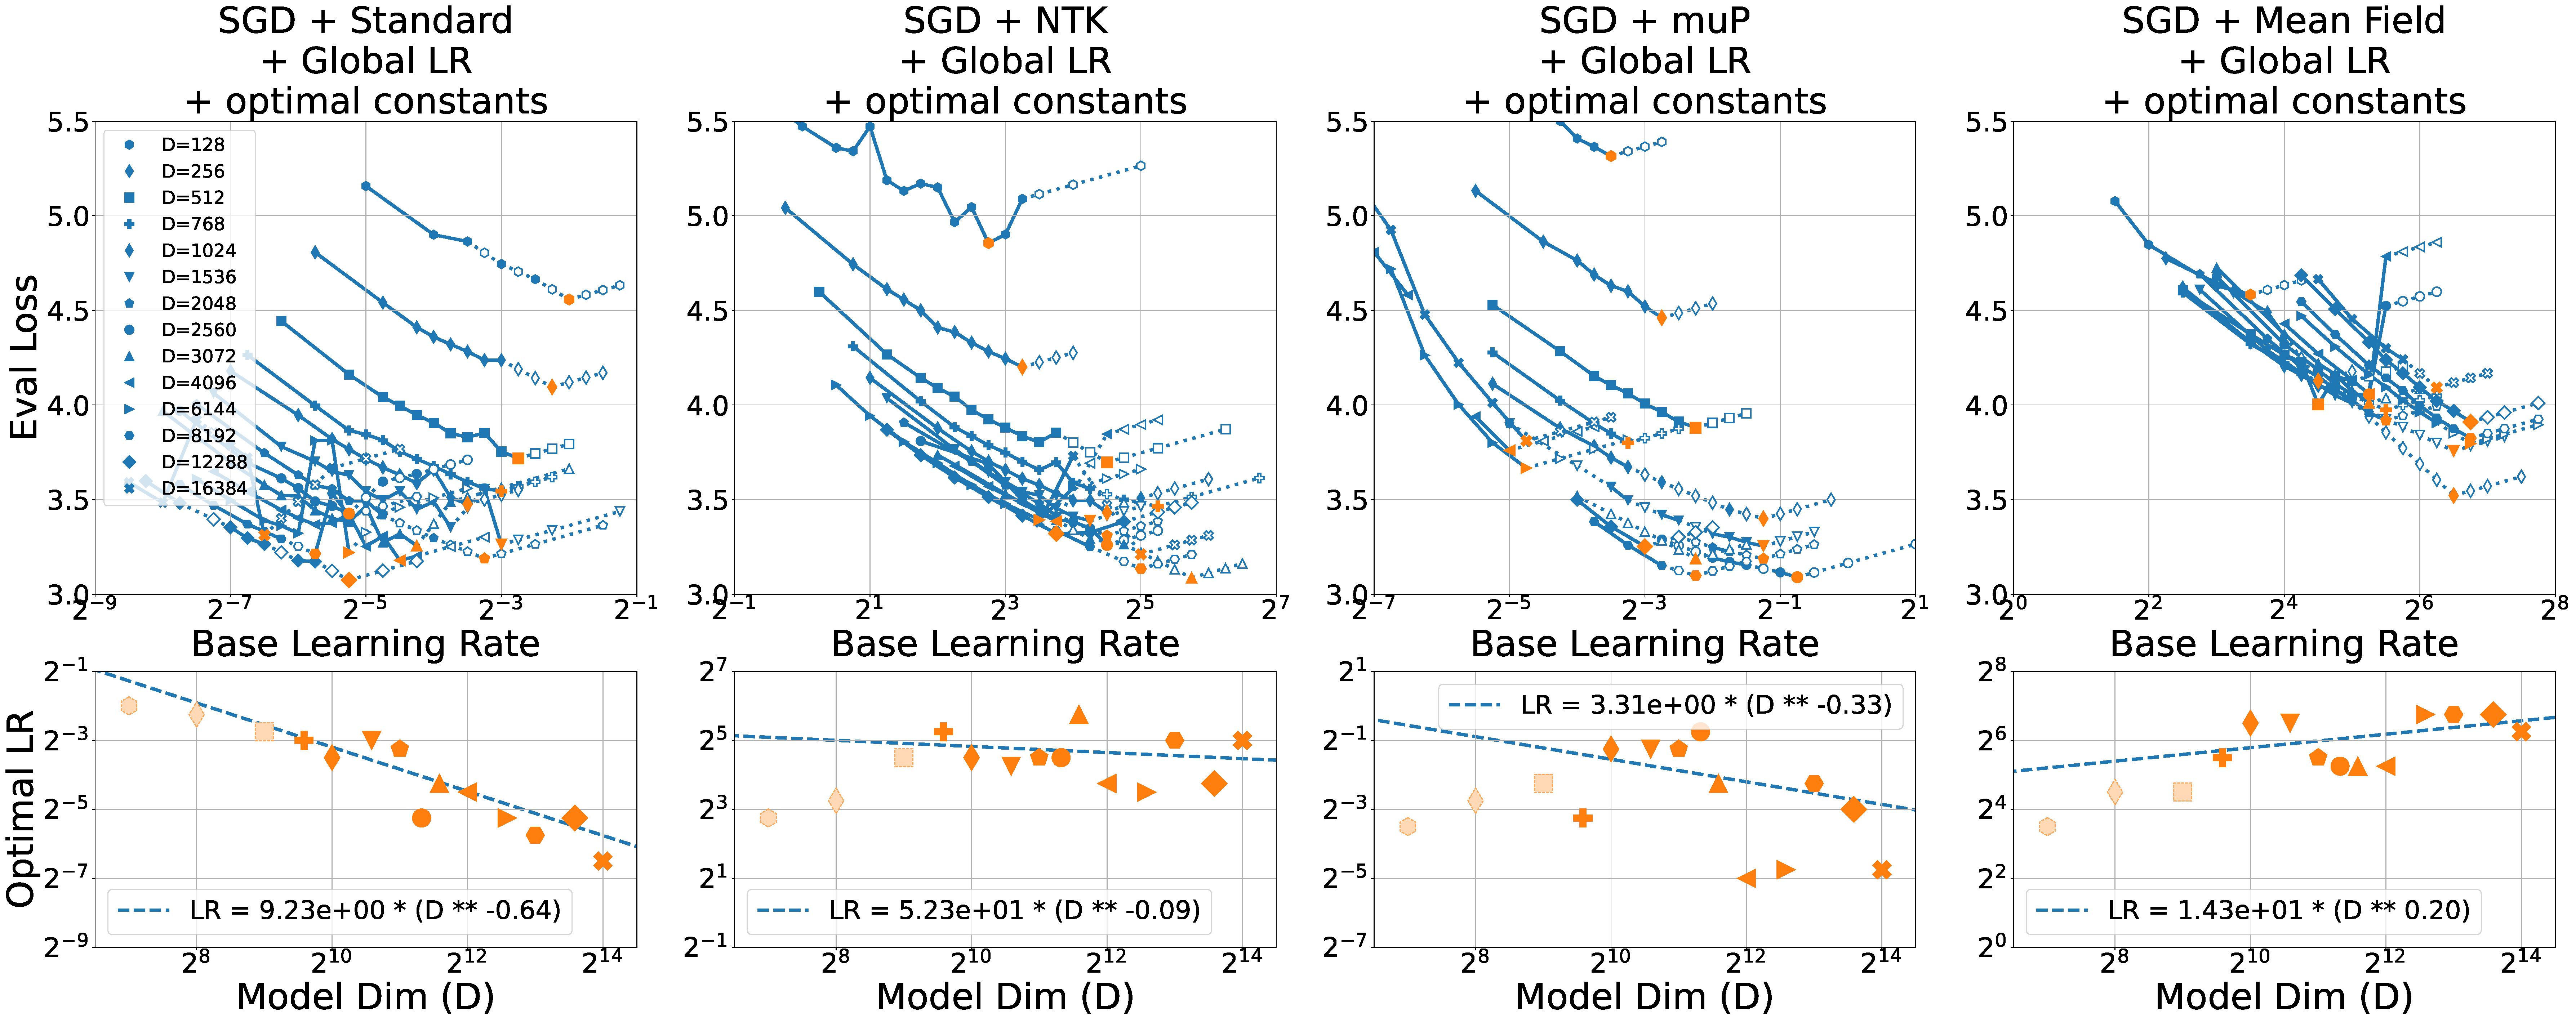
\includegraphics[width=0.98\linewidth]{icml2024/figures/lr_sweeps/appendix/sgd/sgd+50k_steps_optimal_constants_only.pdf}
\caption{Learning rate sweeps and power laws fit to optimal learning rate vs model dim. Top = SGD + global learning rate + default constants. Bottom = SGD + global learning rate + optimal constants. Number of training steps = $50{,}000$.}
\end{SidewaysFigure}
\clearpage

\thispagestyle{plain}
\begin{SidewaysFigure}
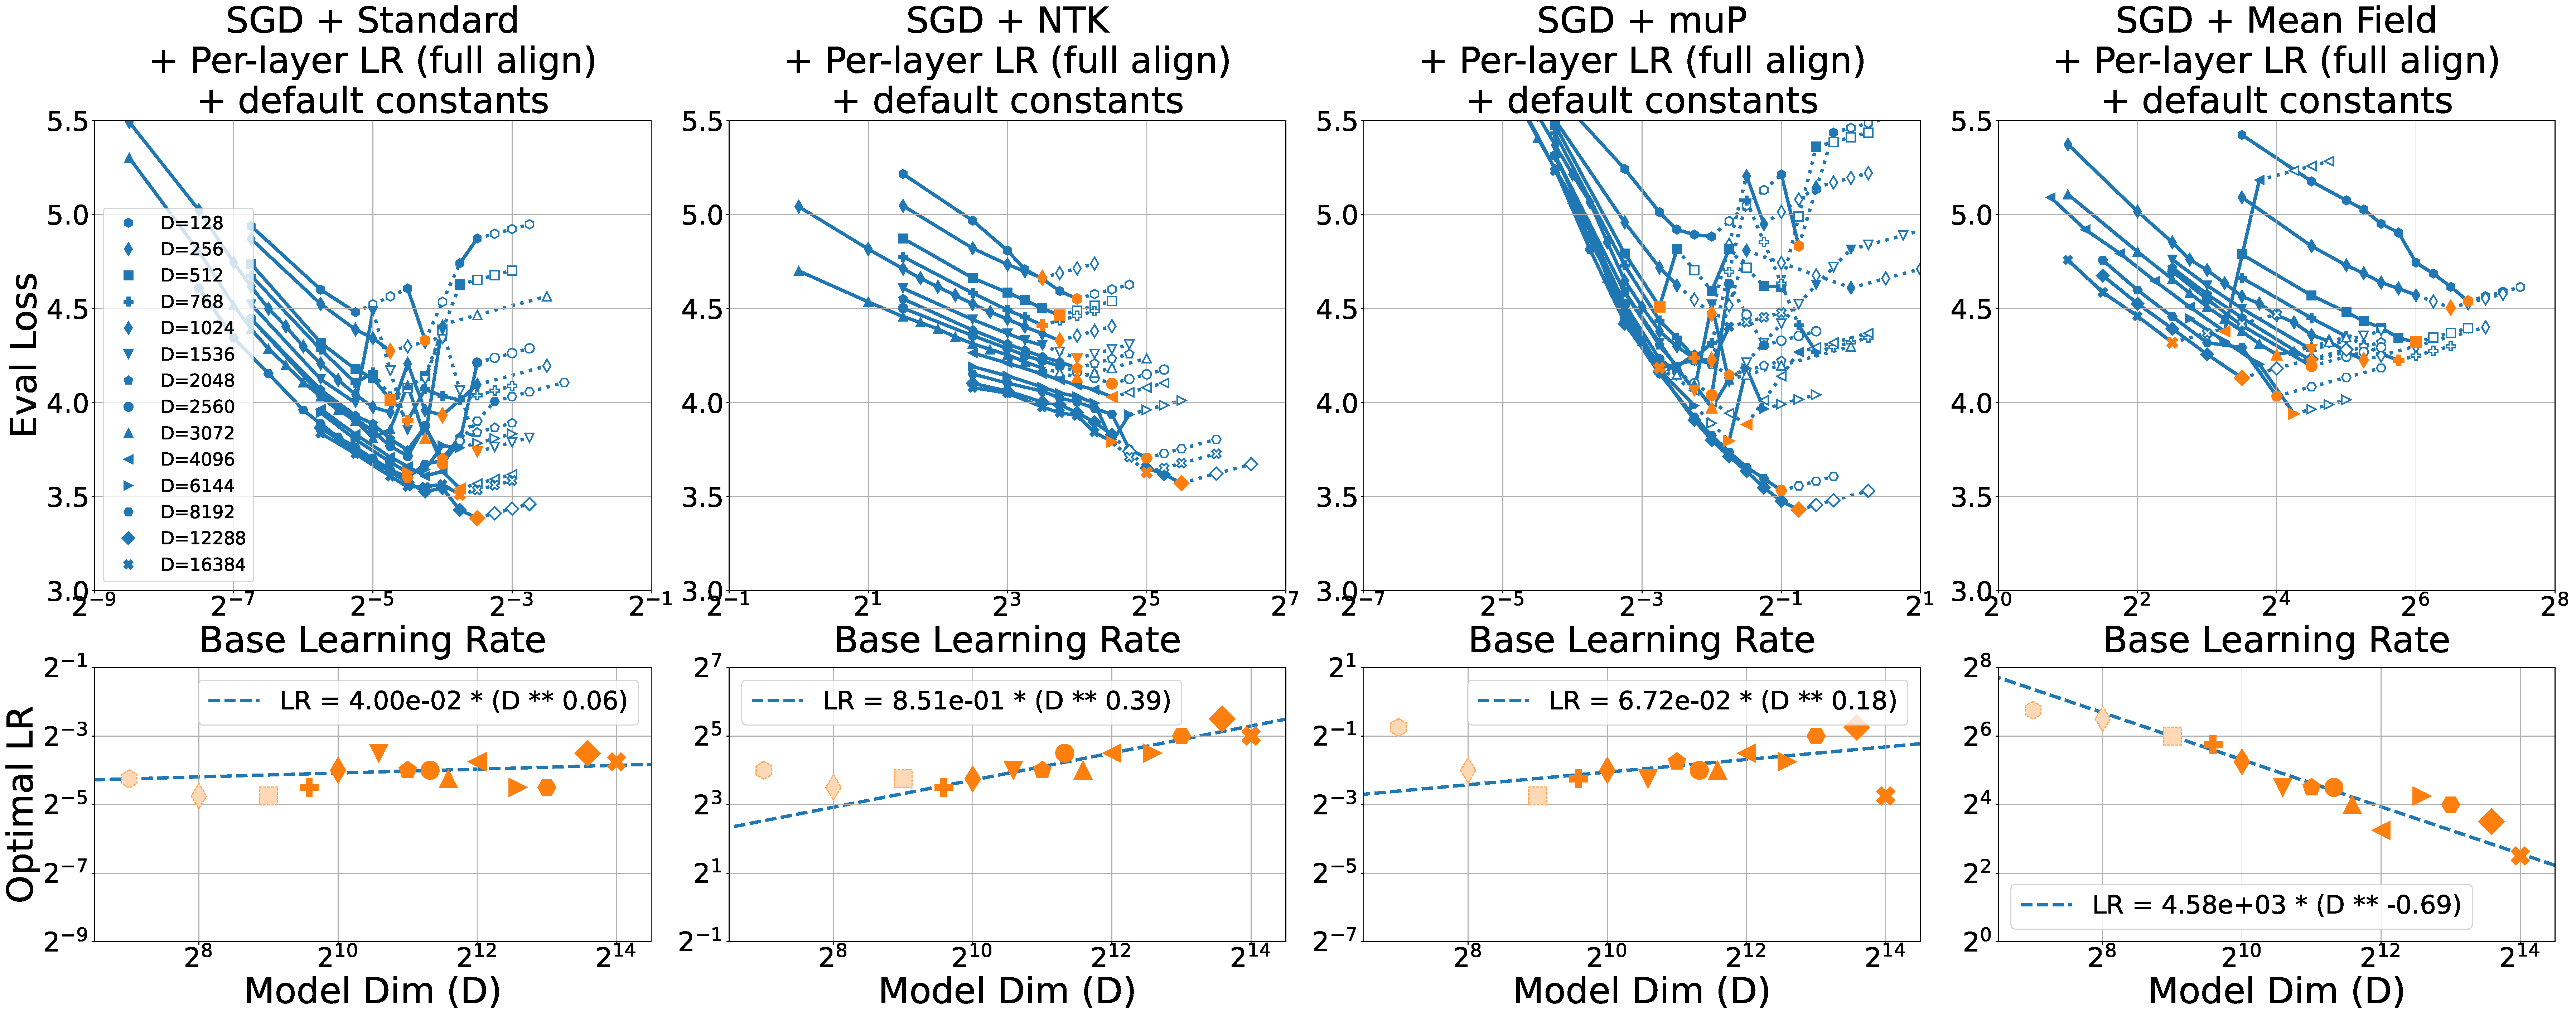
\includegraphics[width=0.98\linewidth]{icml2024/figures/lr_sweeps/appendix/sgd/sgd+50k_steps_per_module_lr.pdf}

\figvspace

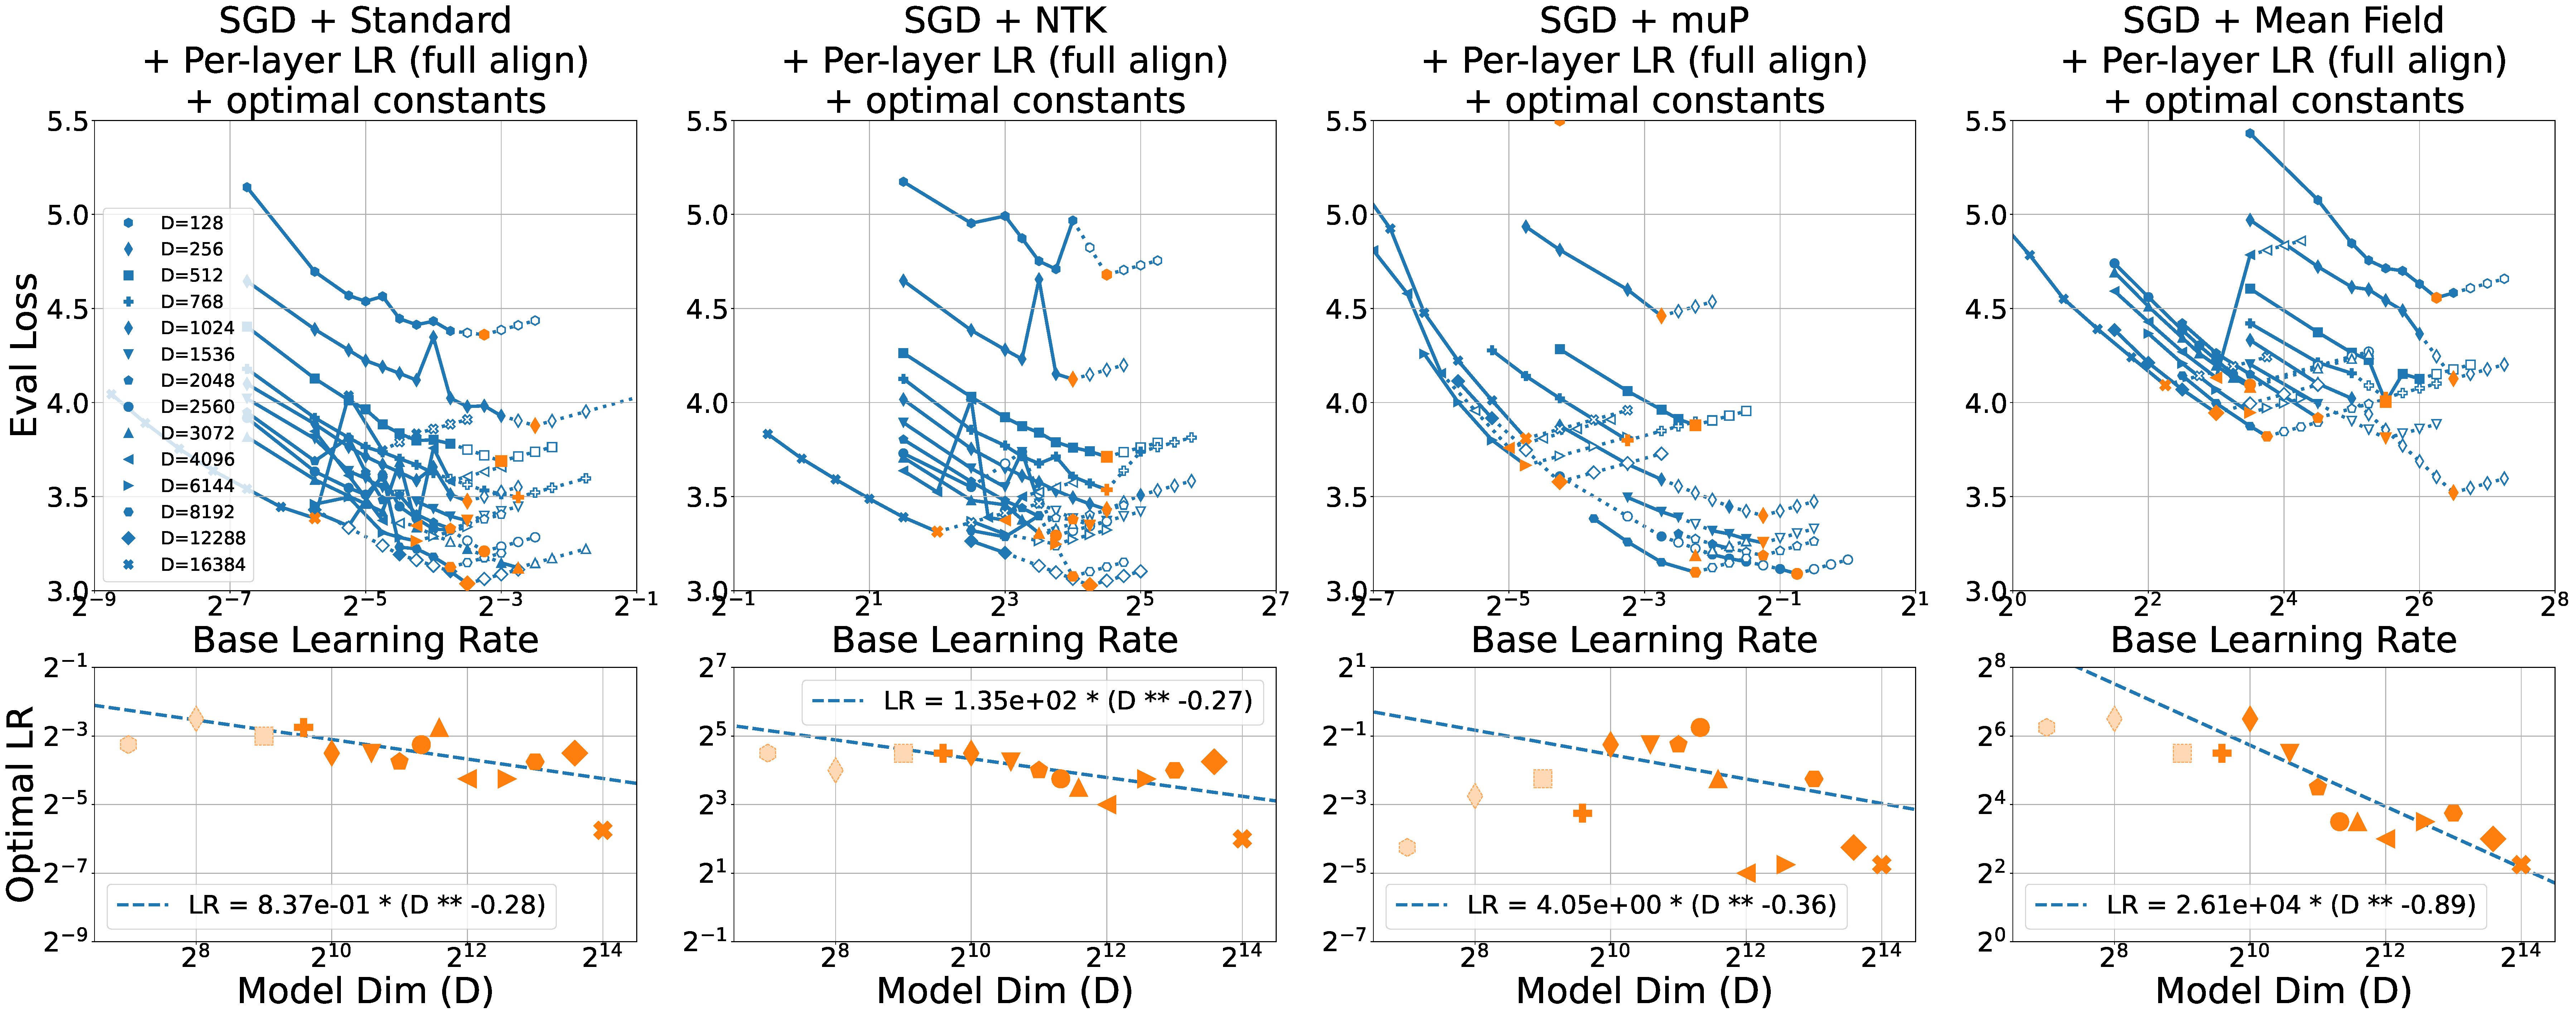
\includegraphics[width=0.98\linewidth]{icml2024/figures/lr_sweeps/appendix/sgd/sgd+50k_steps_per_module_lr_optimal_constants.pdf}
\caption{Learning rate sweeps and power laws fit to optimal learning rate vs model dim. Top = SGD + per-layer learning rate assuming full alignment + default constants. Bottom = SGD + per-layer learning rate assuming full alignment + optimal constants. Number of training steps = $50{,}000$.}
\end{SidewaysFigure}
\clearpage

\thispagestyle{plain}
\begin{SidewaysFigure}
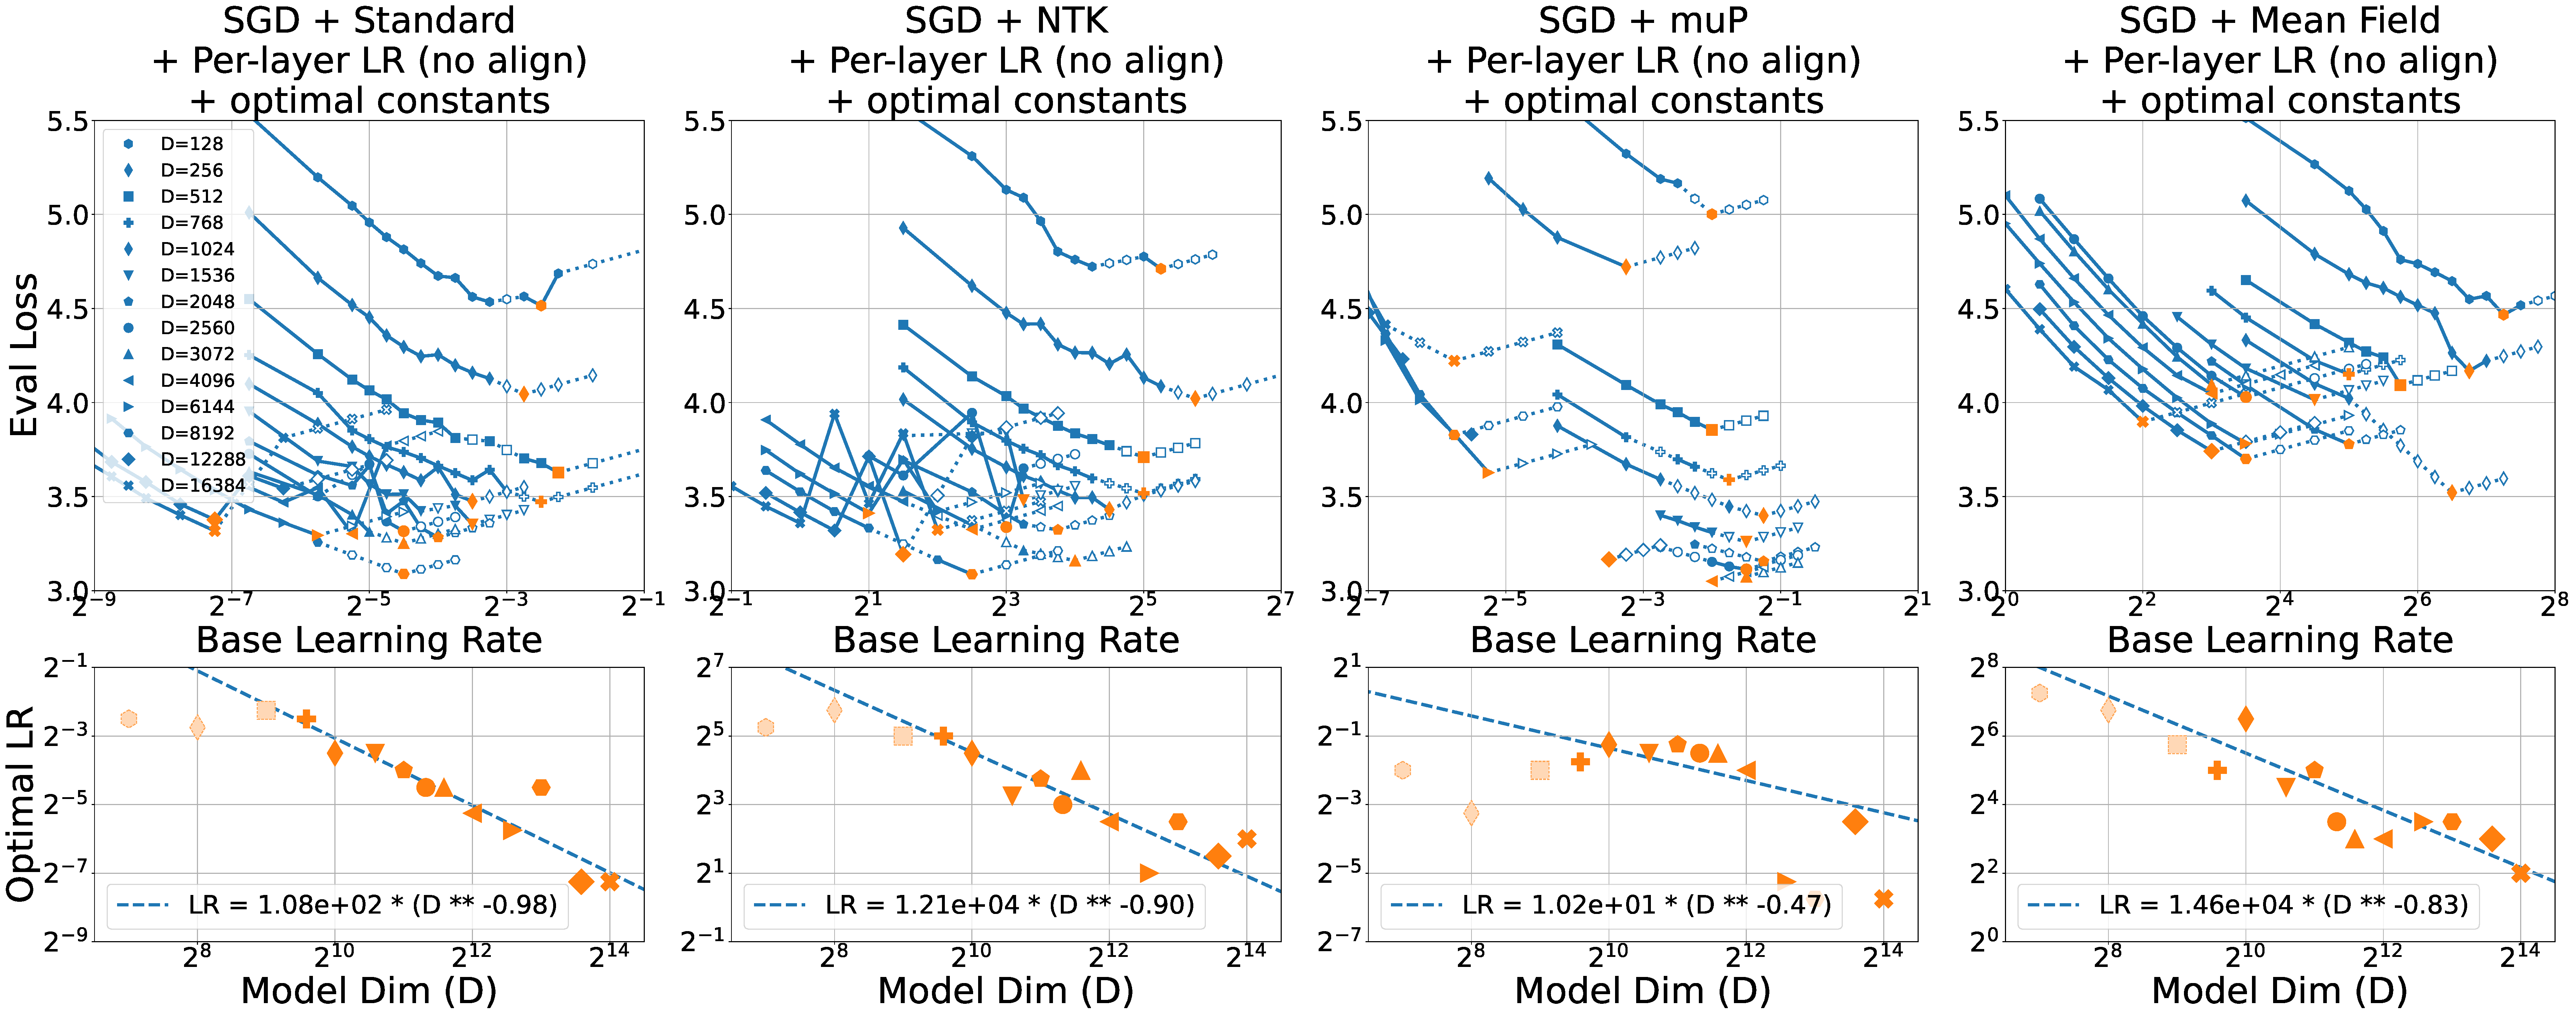
\includegraphics[width=0.98\linewidth]{icml2024/figures/lr_sweeps/appendix/sgd/sgd+50k_steps_per_module_lr_optimal_constants_no_align.pdf}
\caption{Learning rate sweeps and power laws fit to optimal learning rate vs model dim. SGD + per-layer learning rate assuming no alignment + optimal constants. Number of training steps = $50{,}000$.}
\end{SidewaysFigure}
\clearpage

\clearpage
\thispagestyle{plain}
\begin{SidewaysFigure}
\subsection{Learning Rate Sweeps for Adam, all settings}
\label{sec:app_lr_sweeps_adam}
\vspace{12pt}
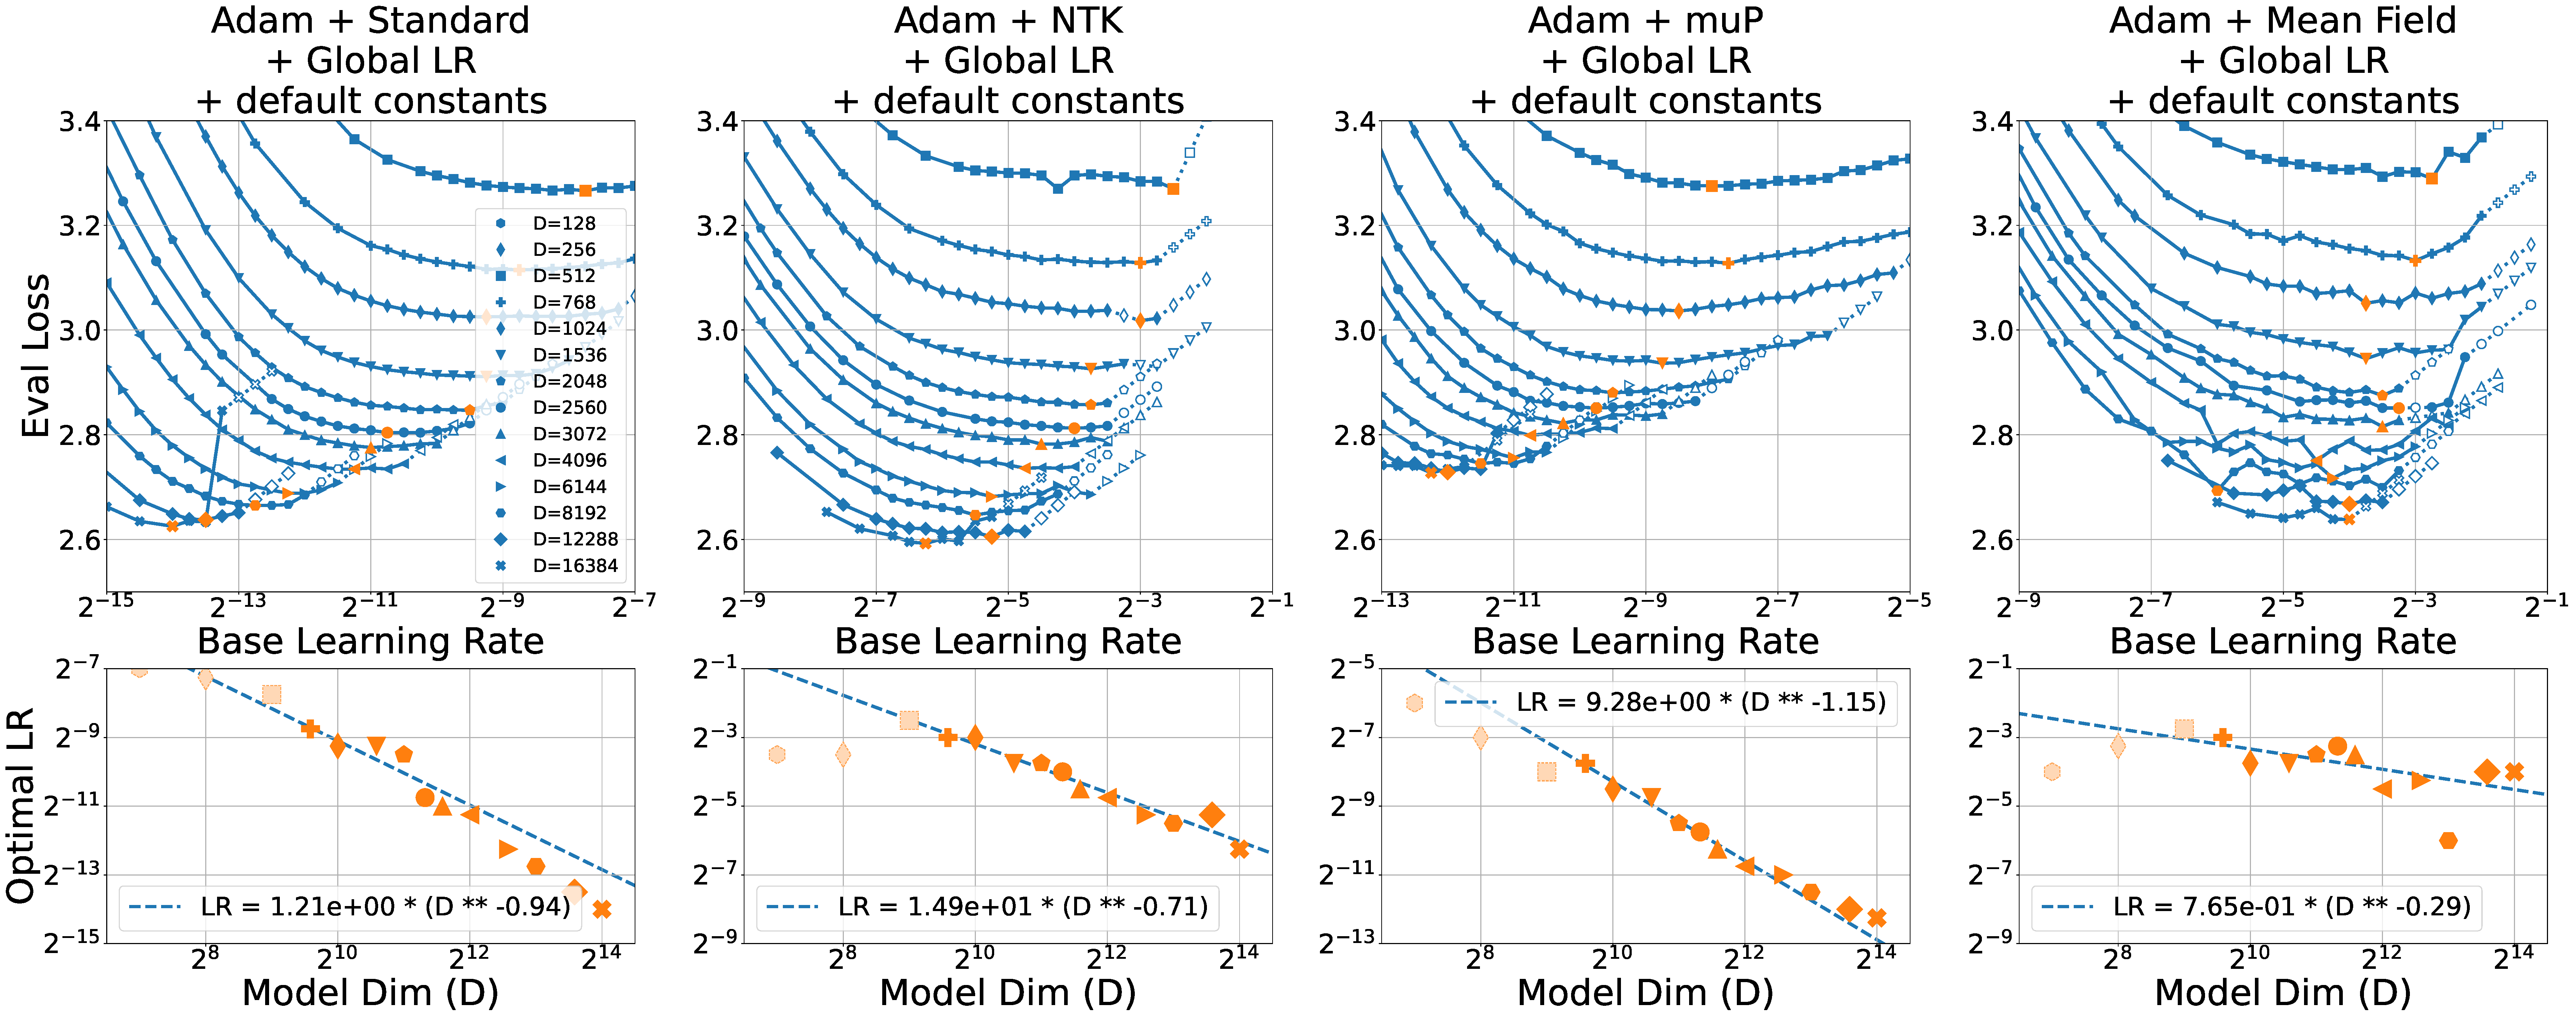
\includegraphics[width=0.98\linewidth]{icml2024/figures/lr_sweeps/appendix/adam/adam+50k_steps.pdf}

\figvspace

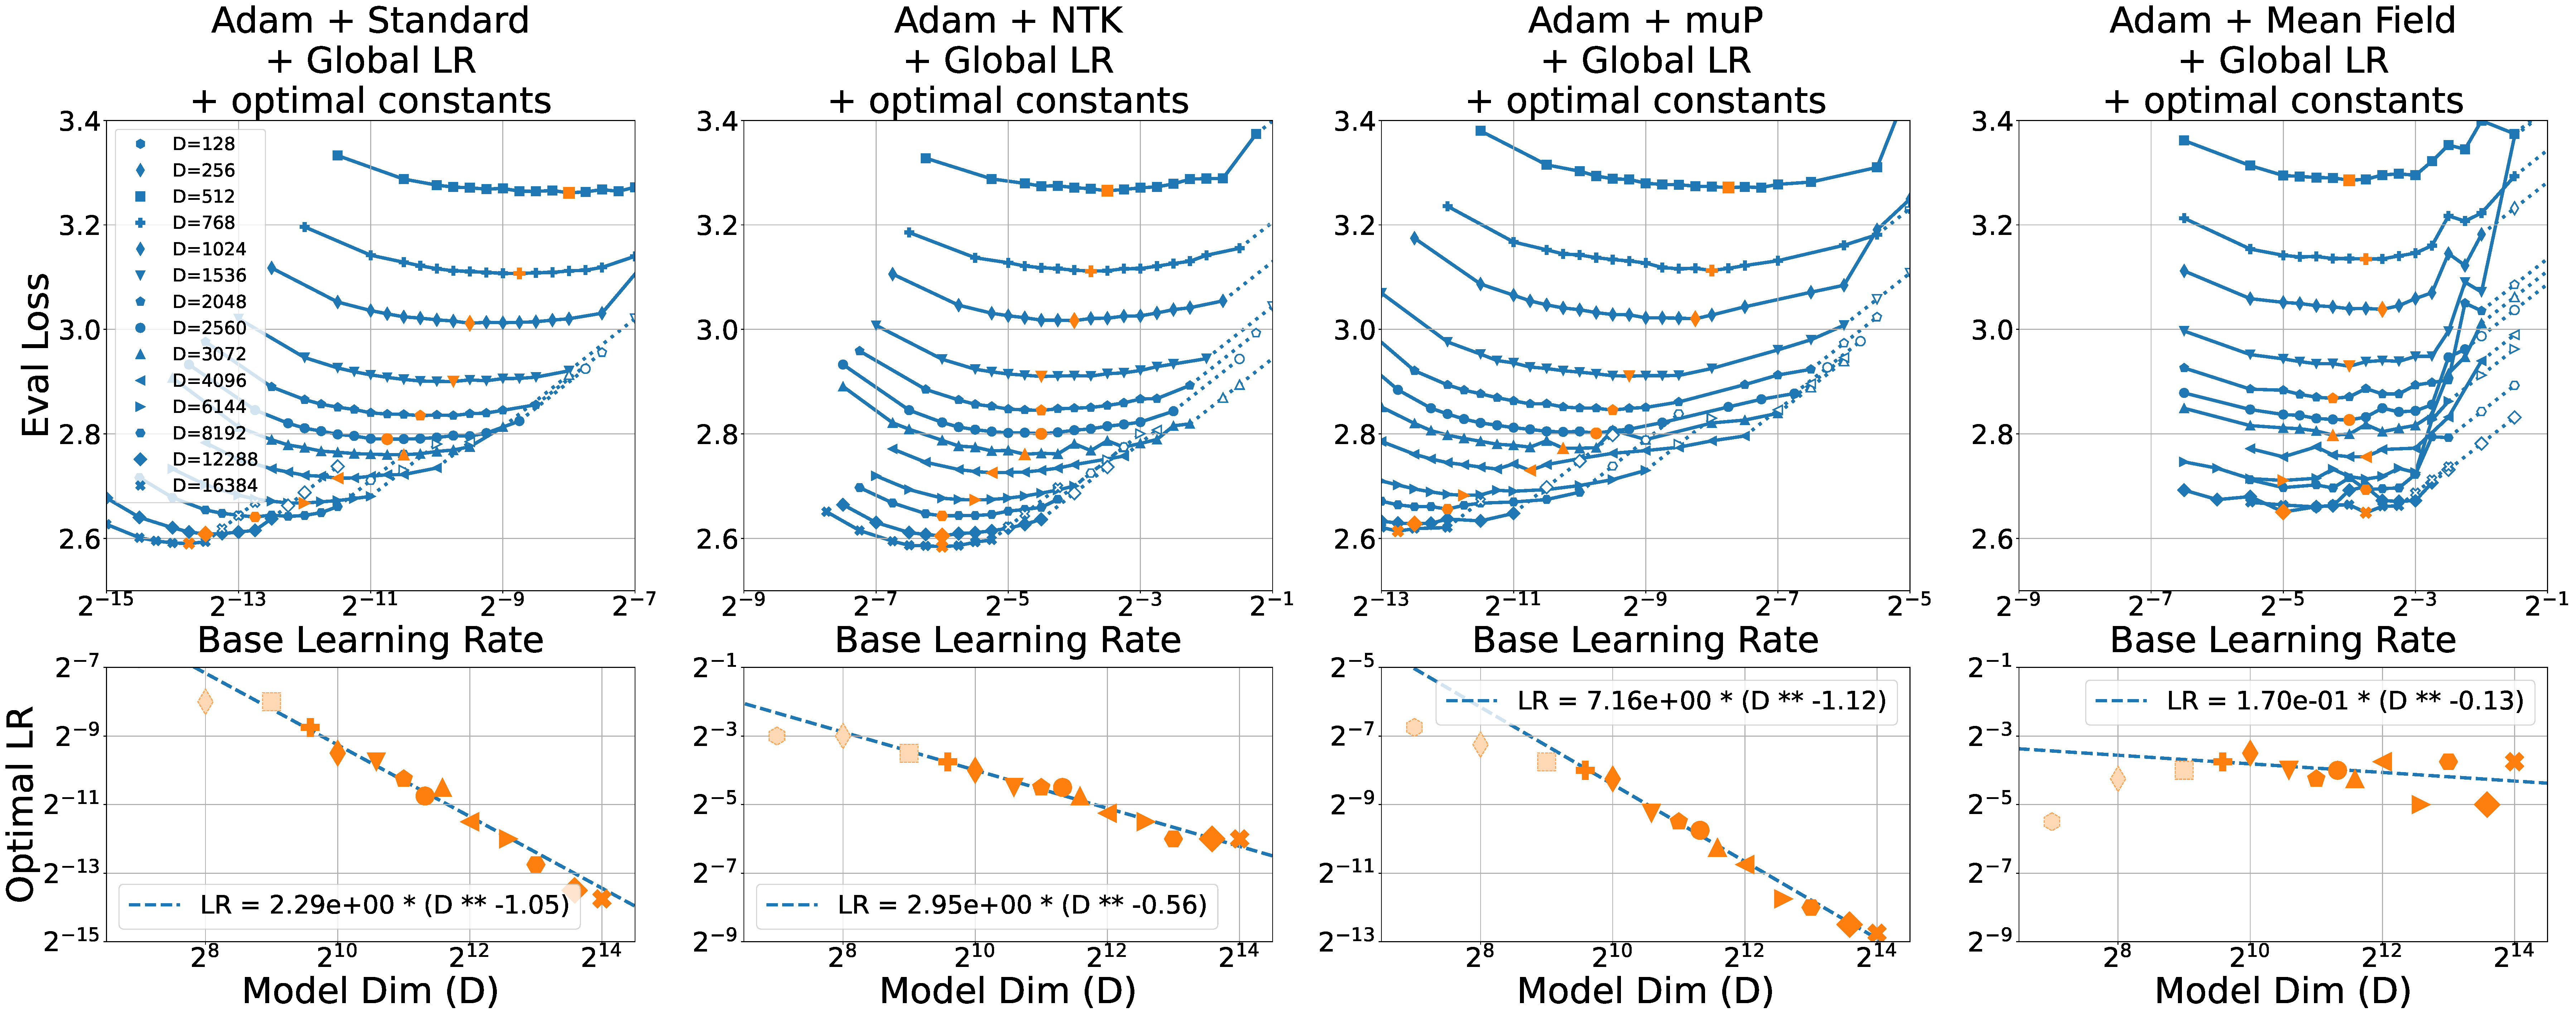
\includegraphics[width=0.98\linewidth]{icml2024/figures/lr_sweeps/appendix/adam/adam+50k_steps_optimal_constants_only.pdf}
\caption{Learning rate sweeps and power laws fit to optimal learning rate vs model dim. Top = Adam + global learning rate + default constants. Bottom = Adam + global learning rate + optimal constants. Number of training steps = $50{,}000$.}
\end{SidewaysFigure}
\clearpage

\thispagestyle{plain}
\begin{SidewaysFigure}
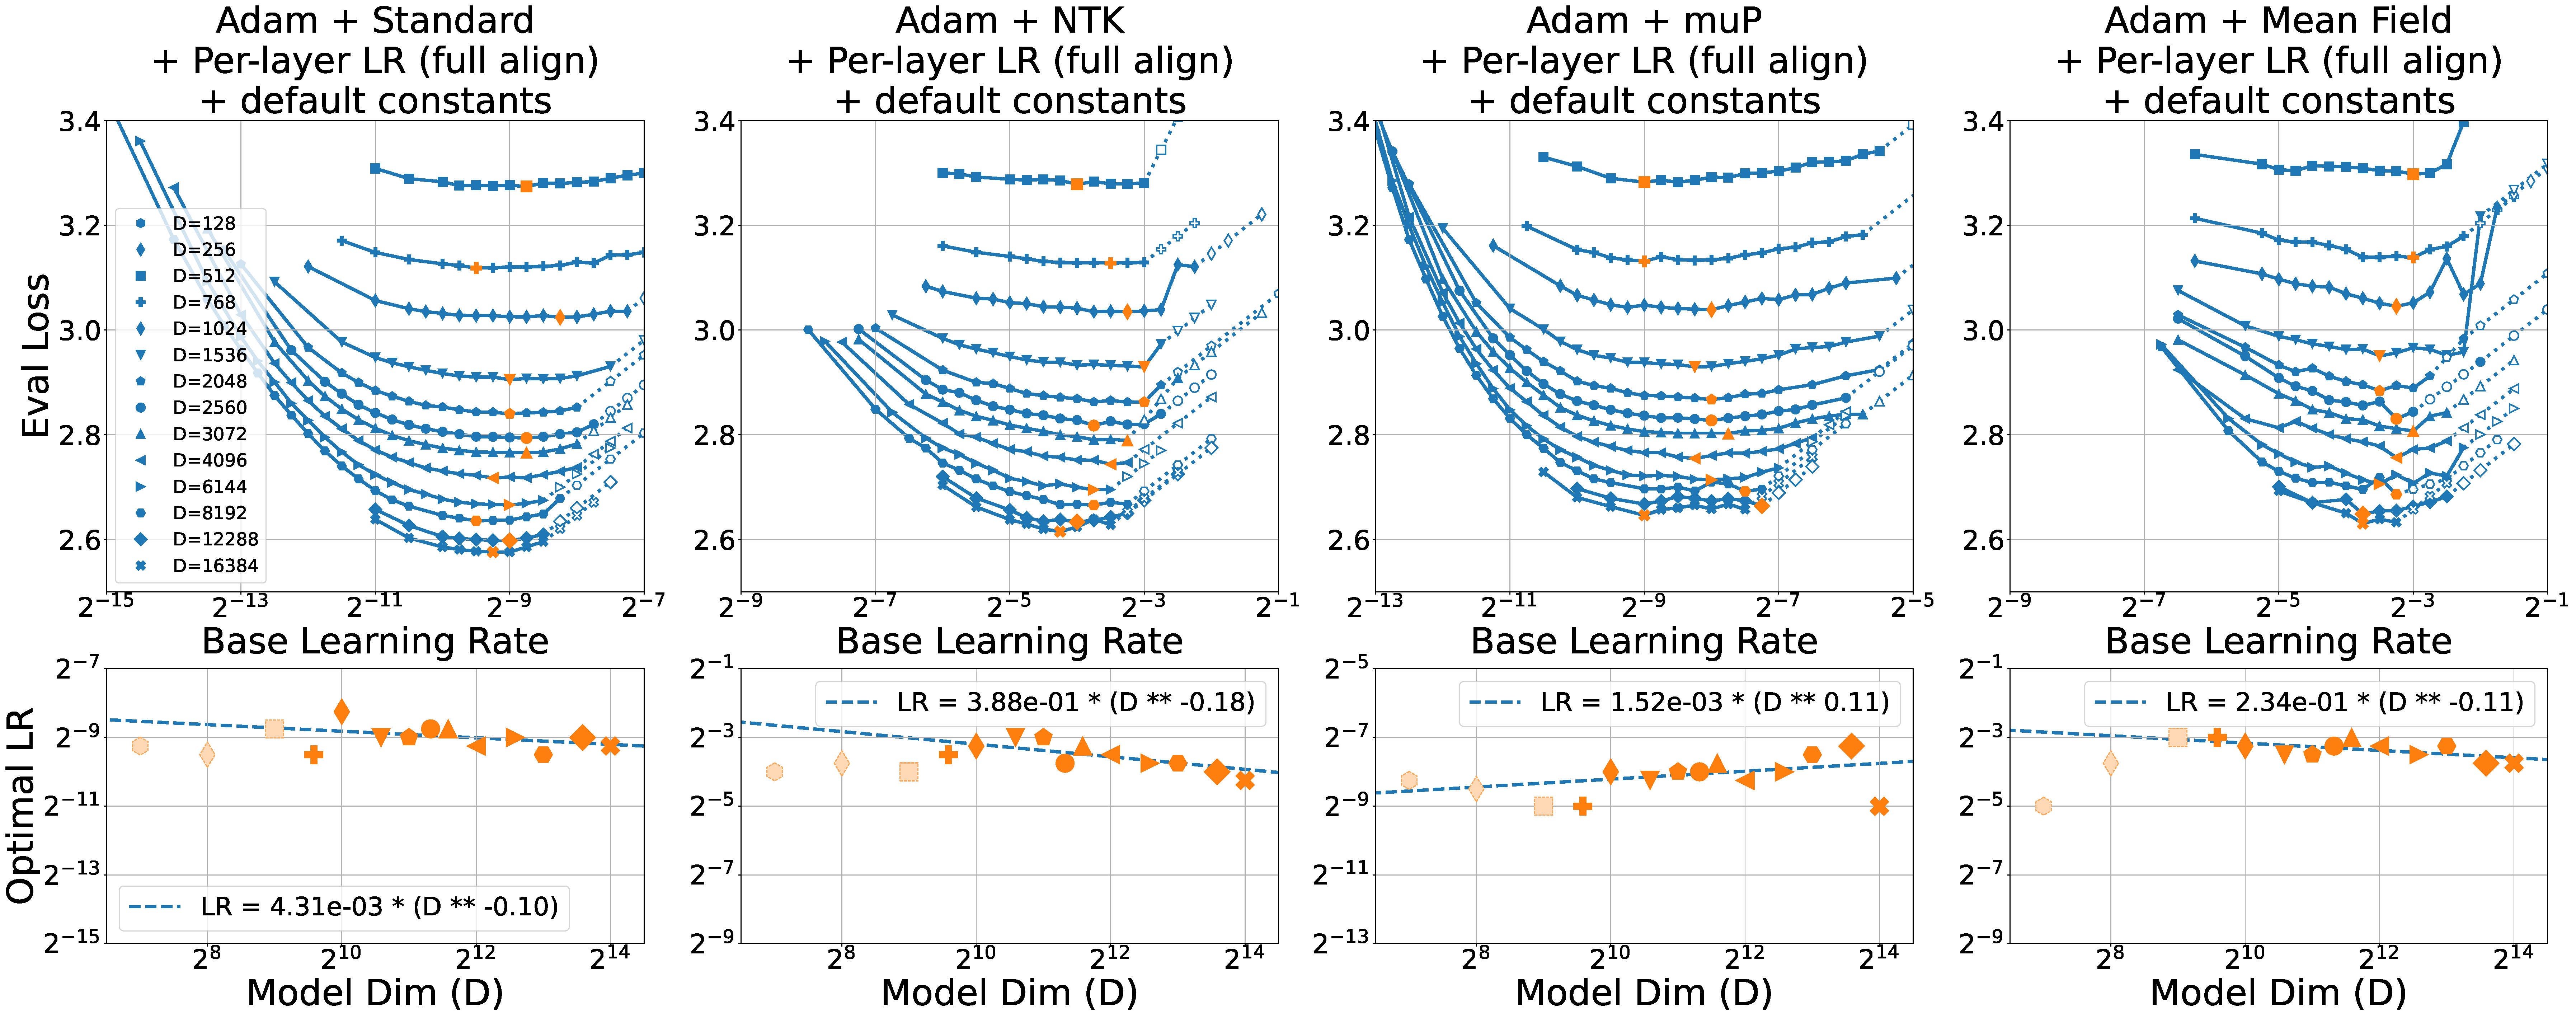
\includegraphics[width=\linewidth]{icml2024/figures/lr_sweeps/appendix/adam/adam+50k_steps_per_module_lr.pdf}

\figvspace

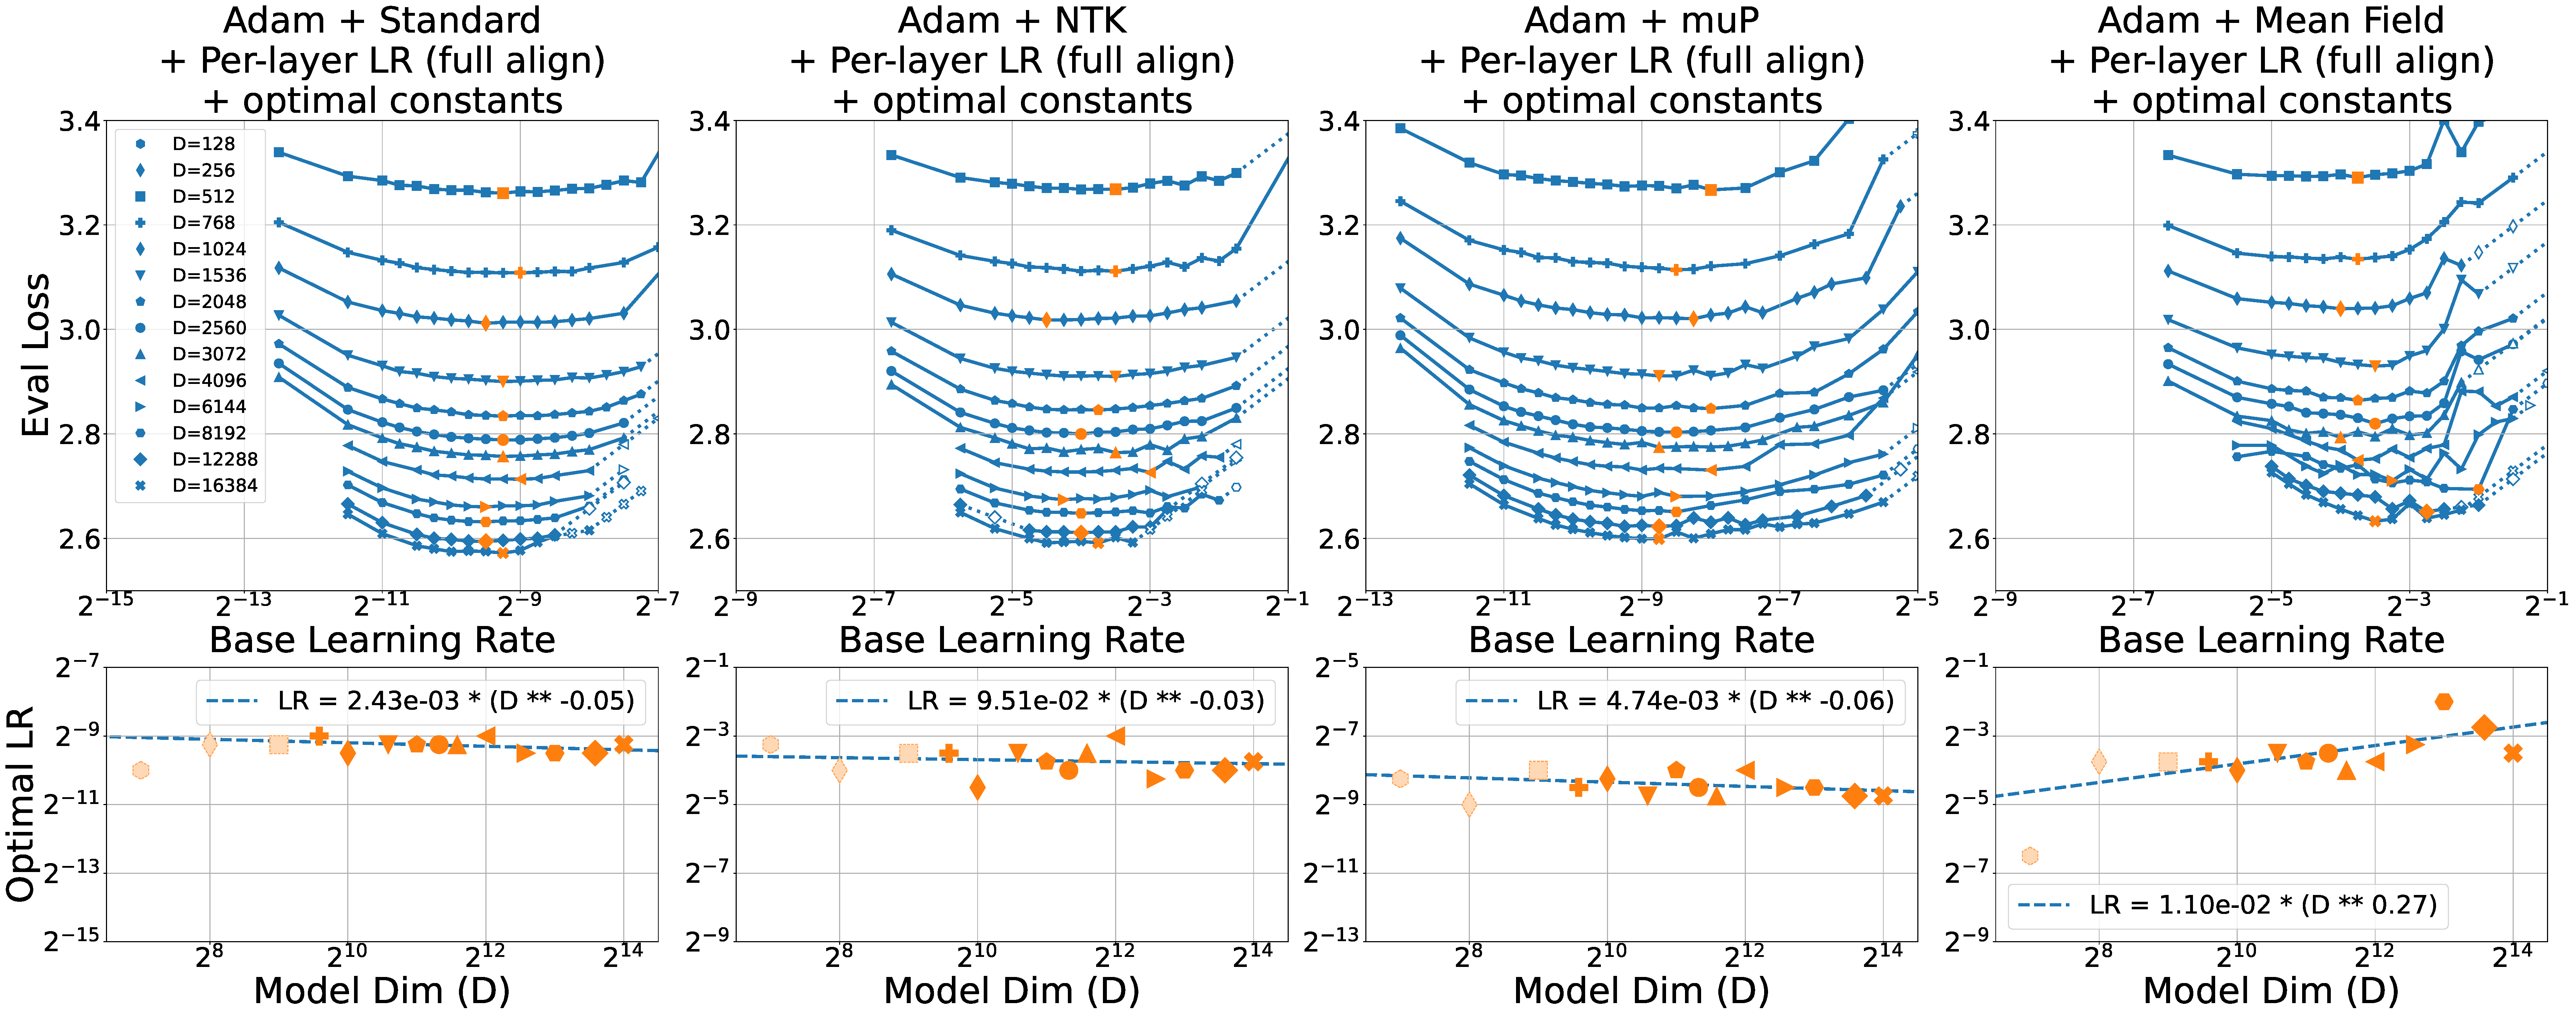
\includegraphics[width=\linewidth]{icml2024/figures/lr_sweeps/appendix/adam/adam+50k_steps_per_module_lr_optimal_constants.pdf}
\caption{Learning rate sweeps and power laws fit to optimal learning rate vs model dim. Top = Adam + per-layer learning rates assuming full alignment + default constants. Bottom = Adam + per-layer learning rates assuming full alignment + optimal constants. Number of training steps = $50{,}000$.}
\end{SidewaysFigure}
\clearpage

\thispagestyle{plain}
\begin{SidewaysFigure}
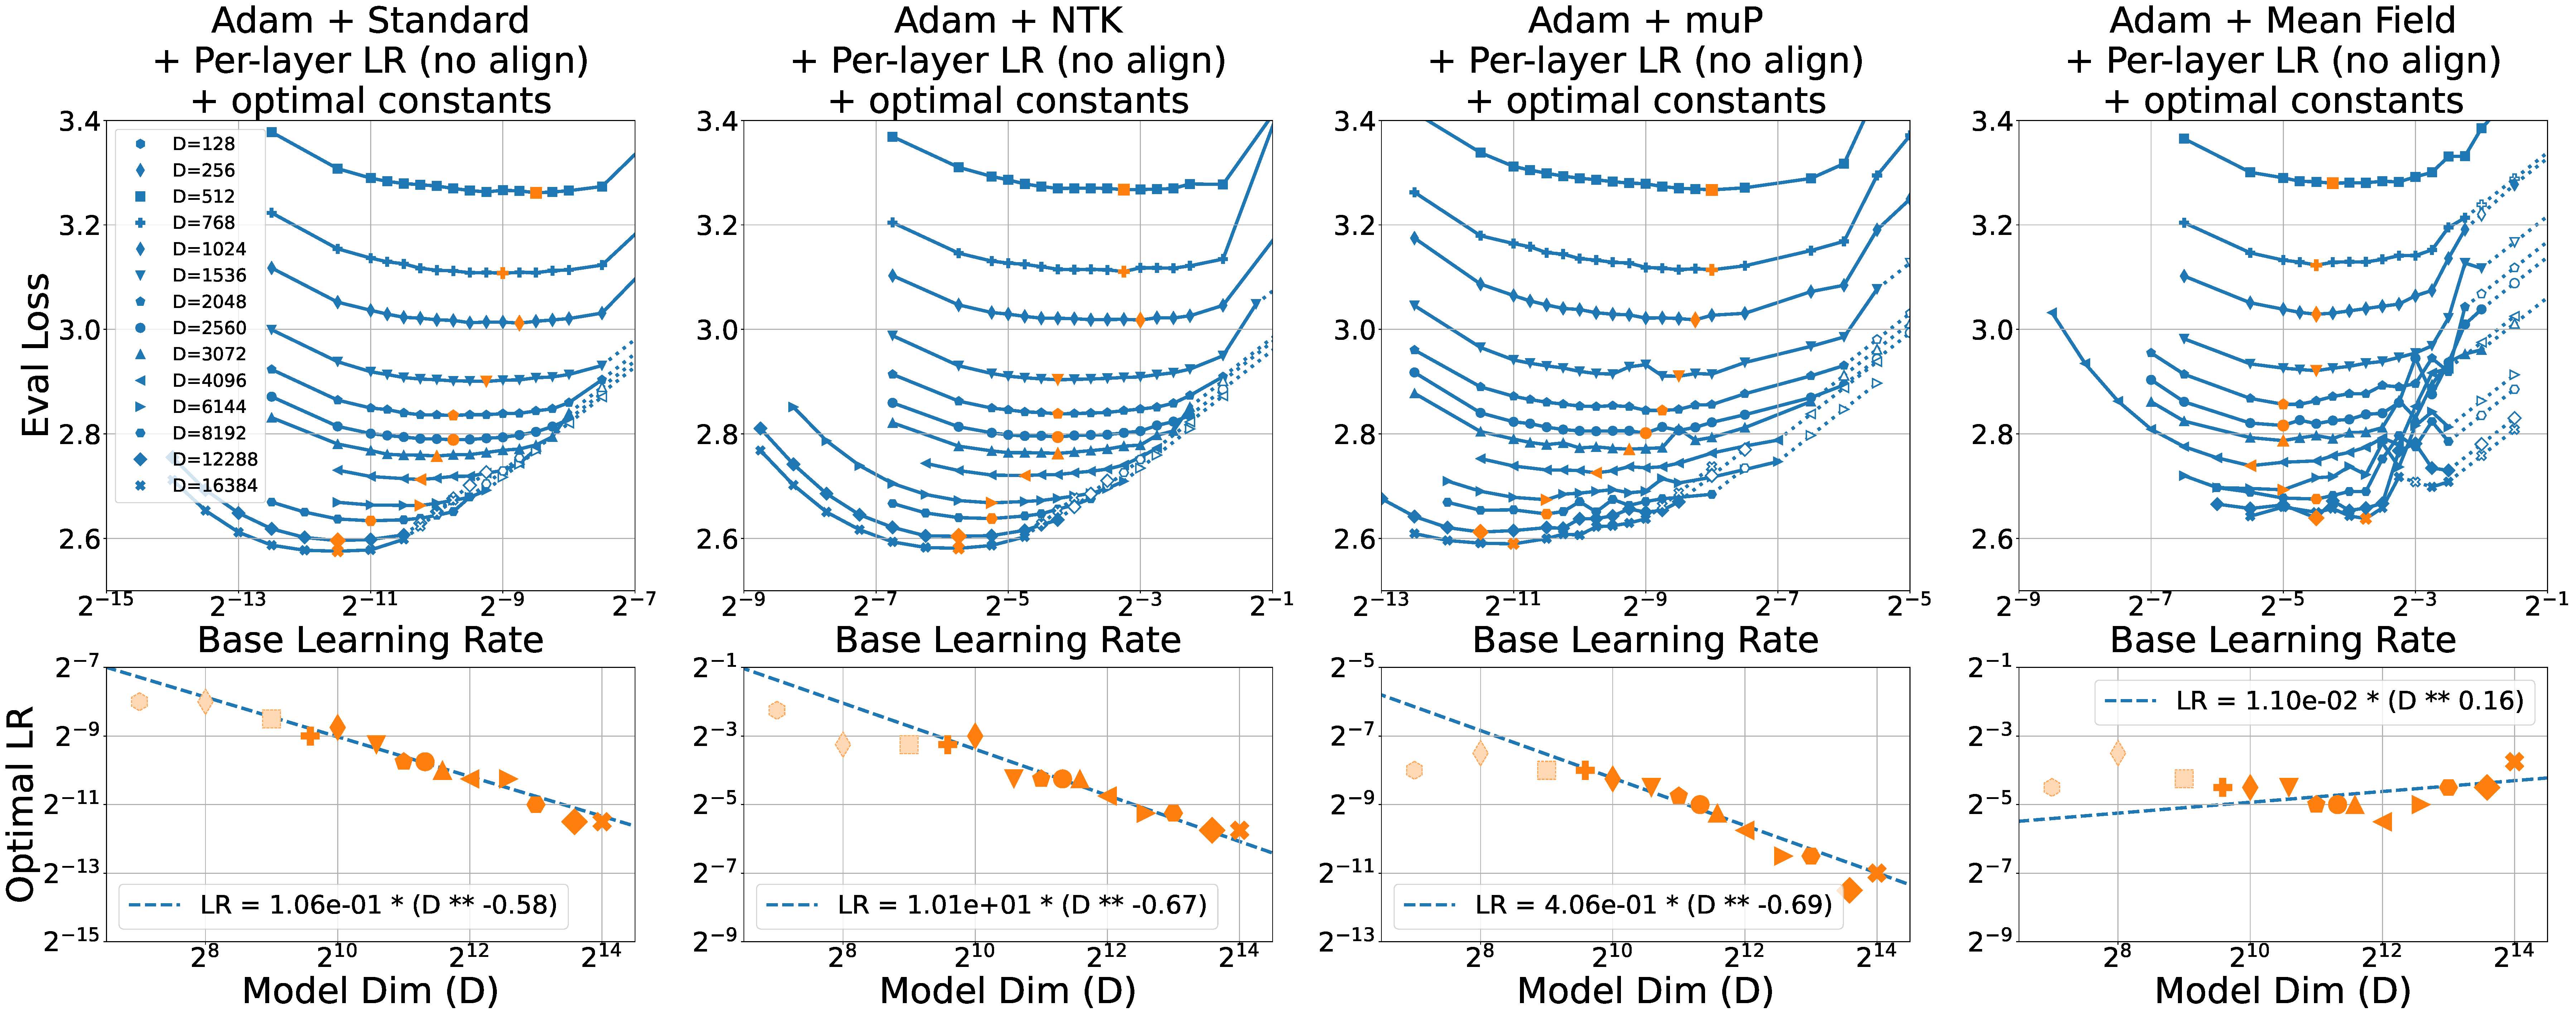
\includegraphics[width=\linewidth]{icml2024/figures/lr_sweeps/appendix/adam/adam+50k_steps_per_module_lr_optimal_constants_no_align.pdf}

\figvspace

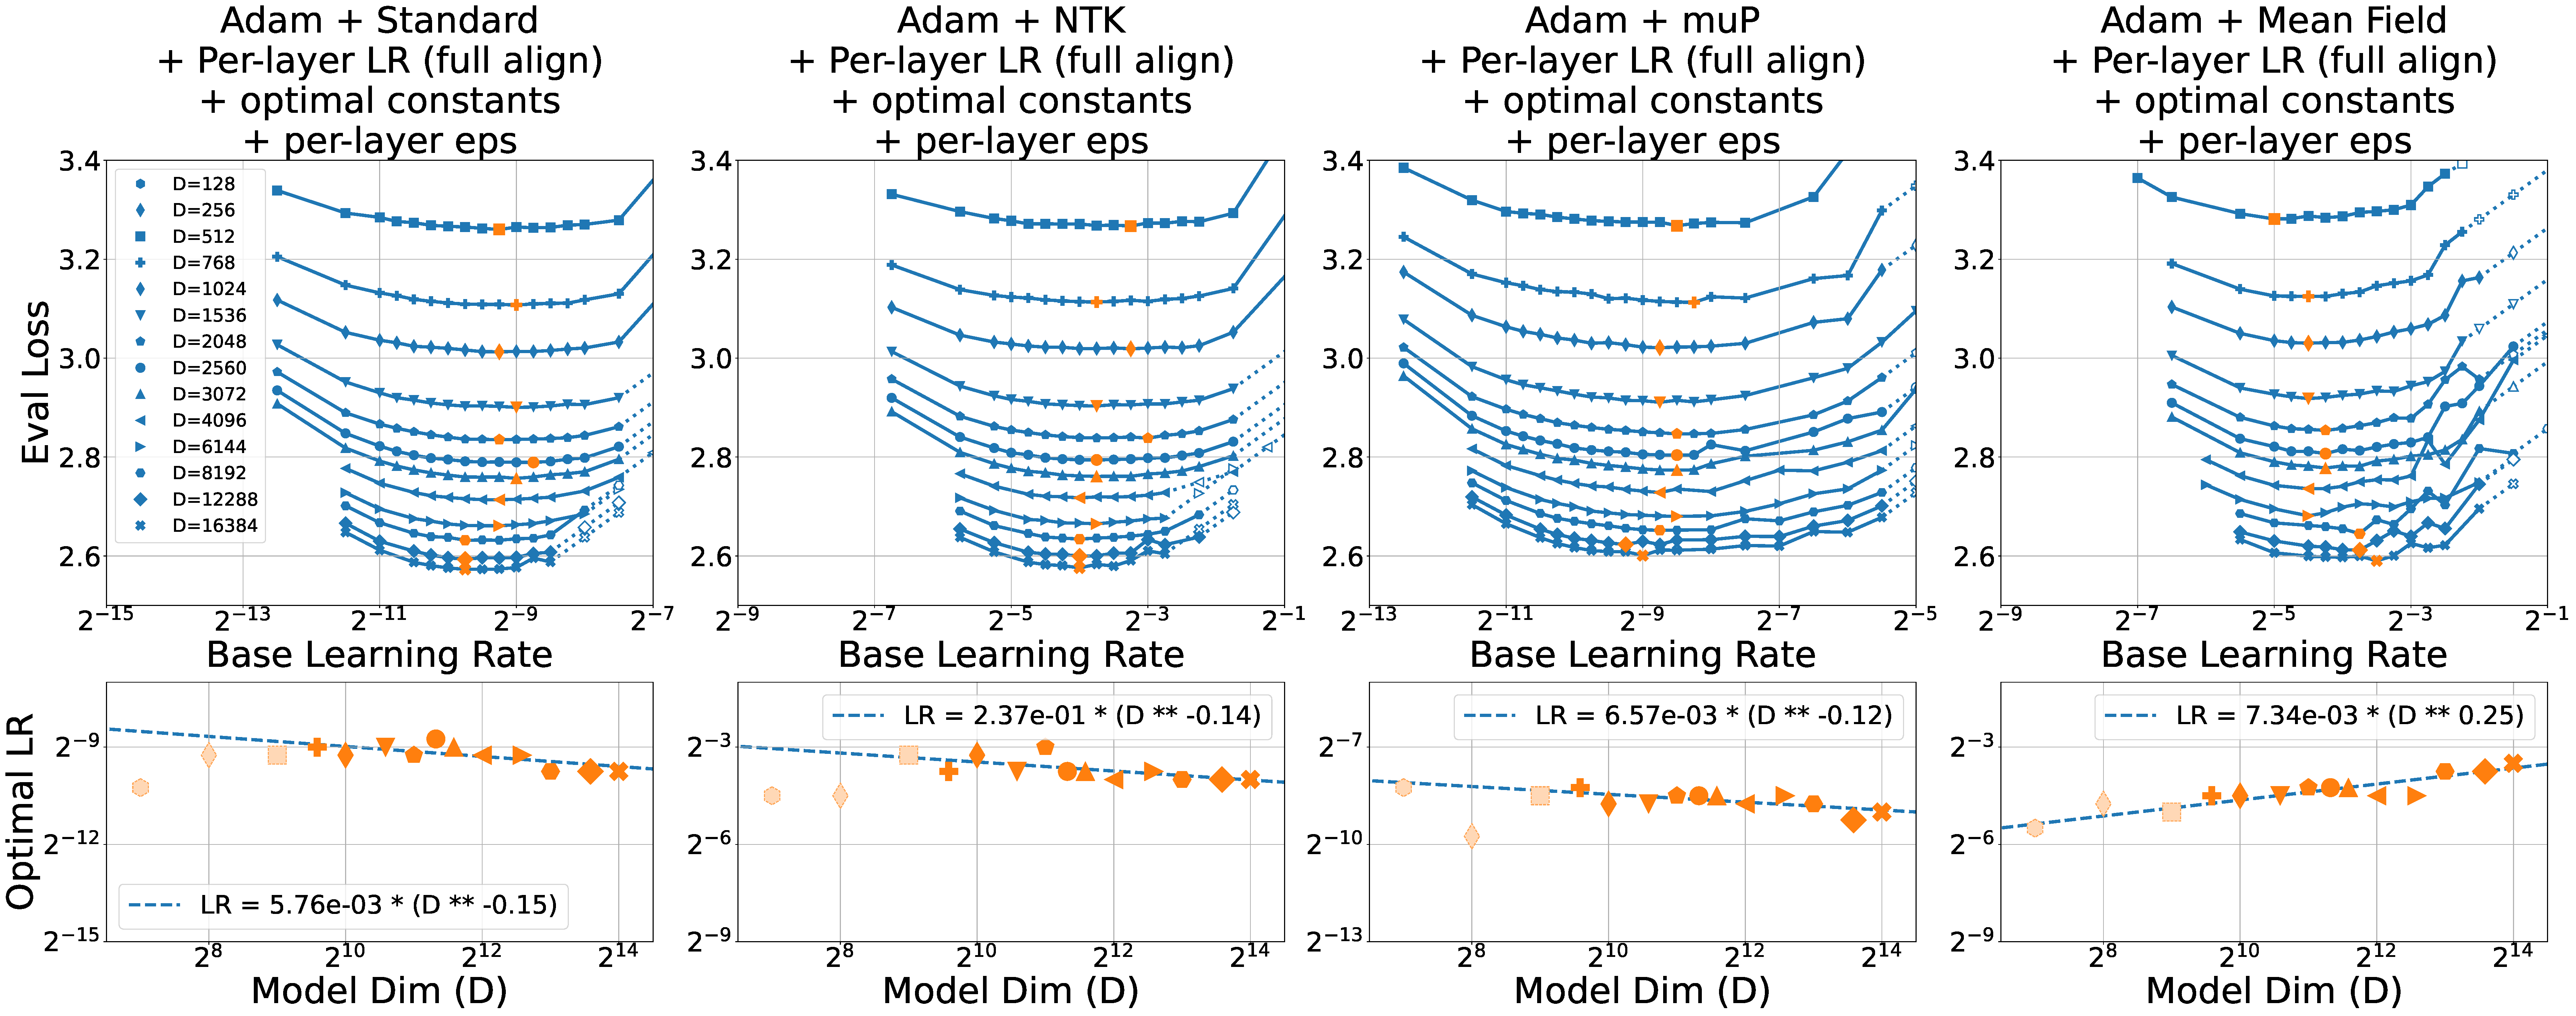
\includegraphics[width=\linewidth]{icml2024/figures/lr_sweeps/appendix/adam/adam+50k_steps_per_module_lr_optimal_constants_per_module_eps_base_eps12.pdf}
\caption{Learning rate sweeps and power laws fit to optimal learning rate vs model dim. Top = Adam + per-layer learning rates assuming no alignment + optimal constants. Bottom = Adam + per-layer learning rates assuming full alignment + optimal constants + per-layer epsilon with base epsilon = 1e-12. Number of training steps = $50{,}000$.}
\end{SidewaysFigure}
\clearpage

\thispagestyle{plain}
\begin{SidewaysFigure}
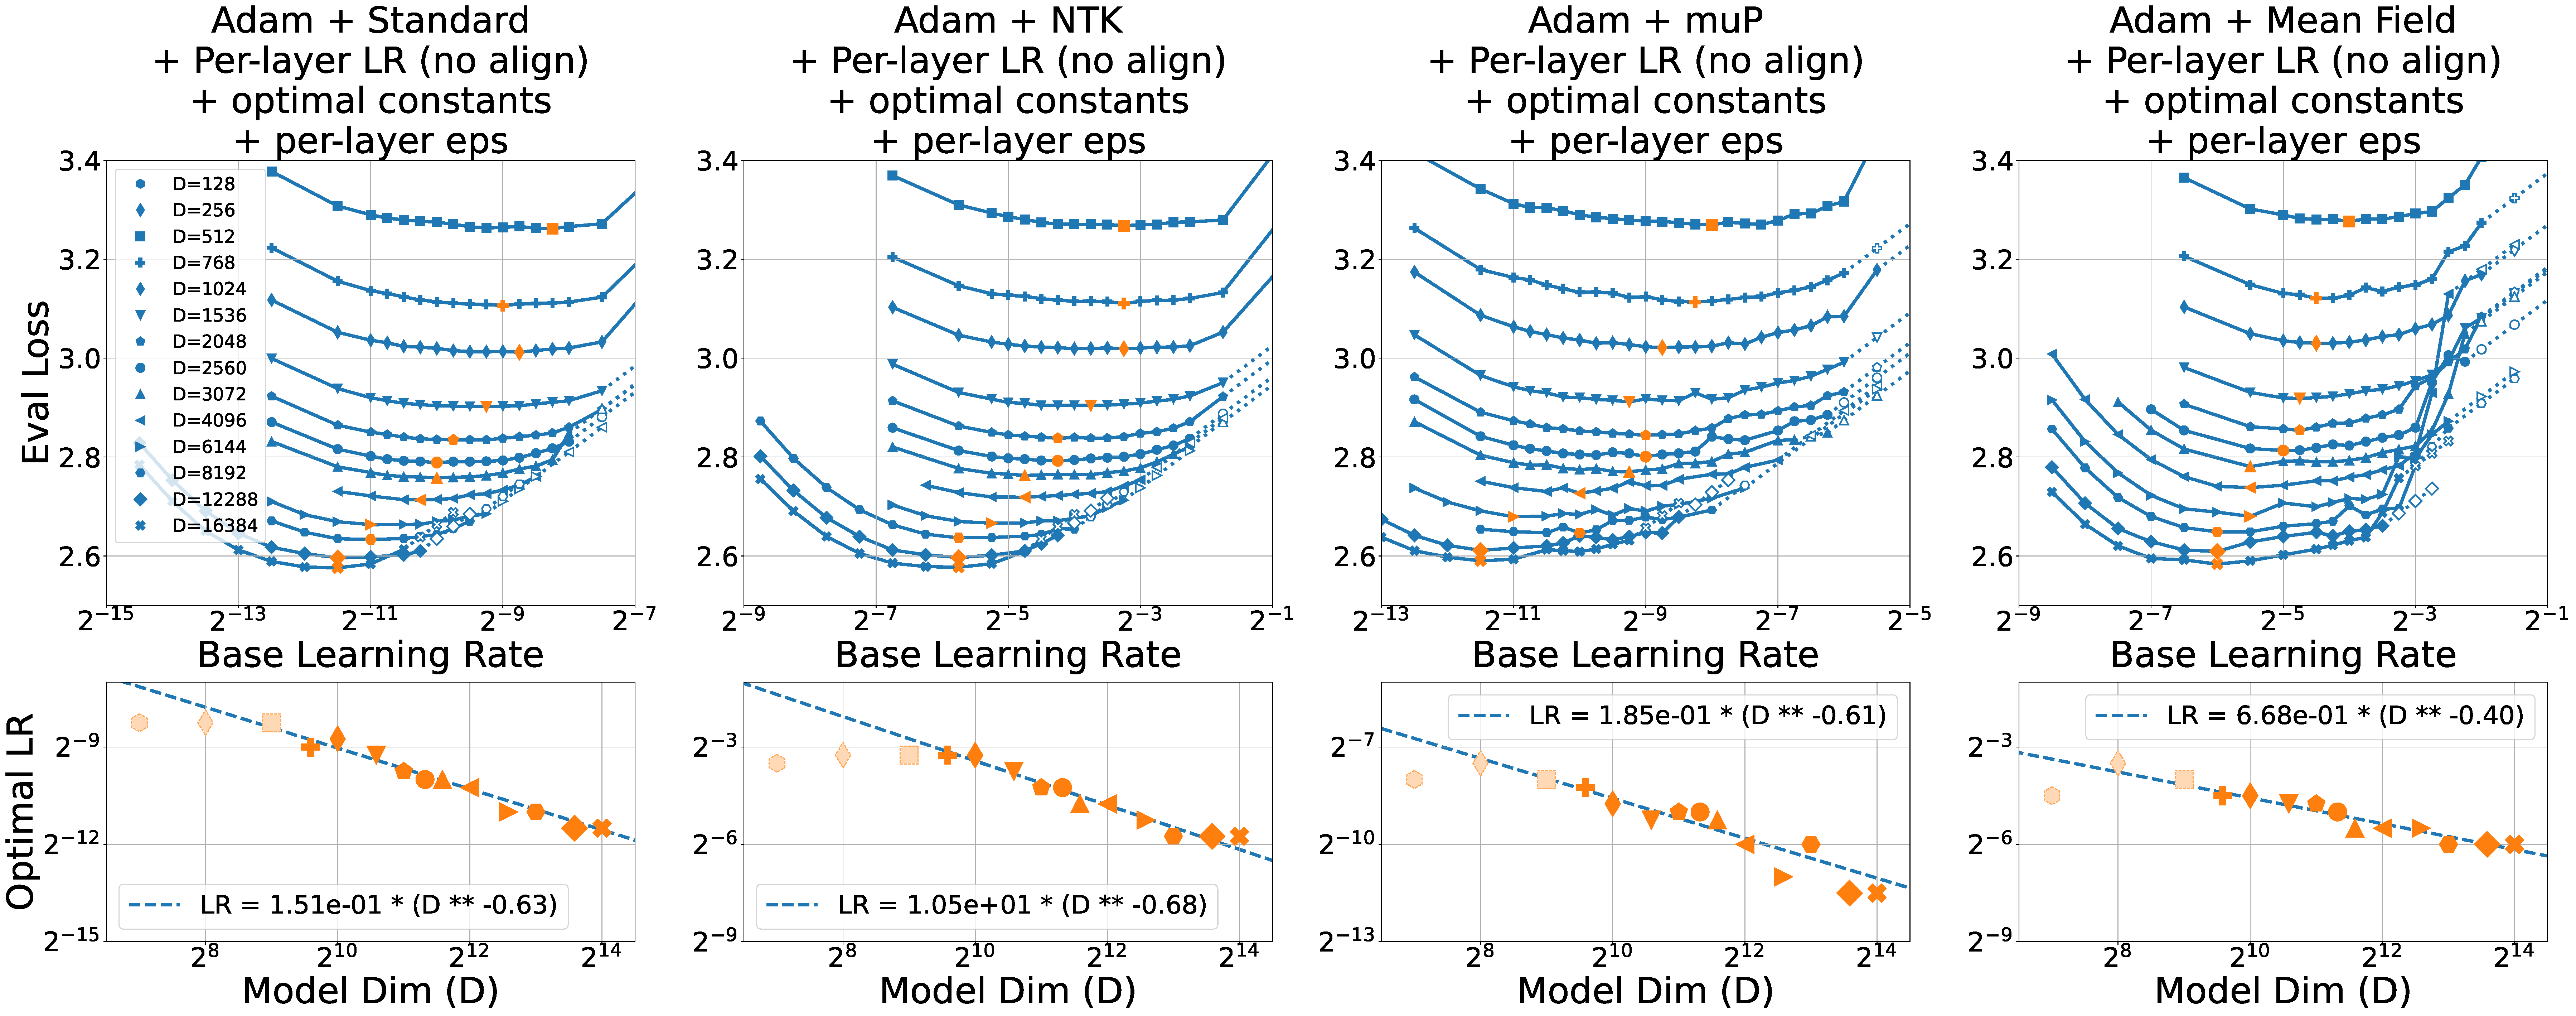
\includegraphics[width=\linewidth]{icml2024/figures/lr_sweeps/appendix/adam/adam+50k_steps_per_module_lr_no_align_optimal_constants_per_module_eps_base_eps12.pdf}

\figvspace

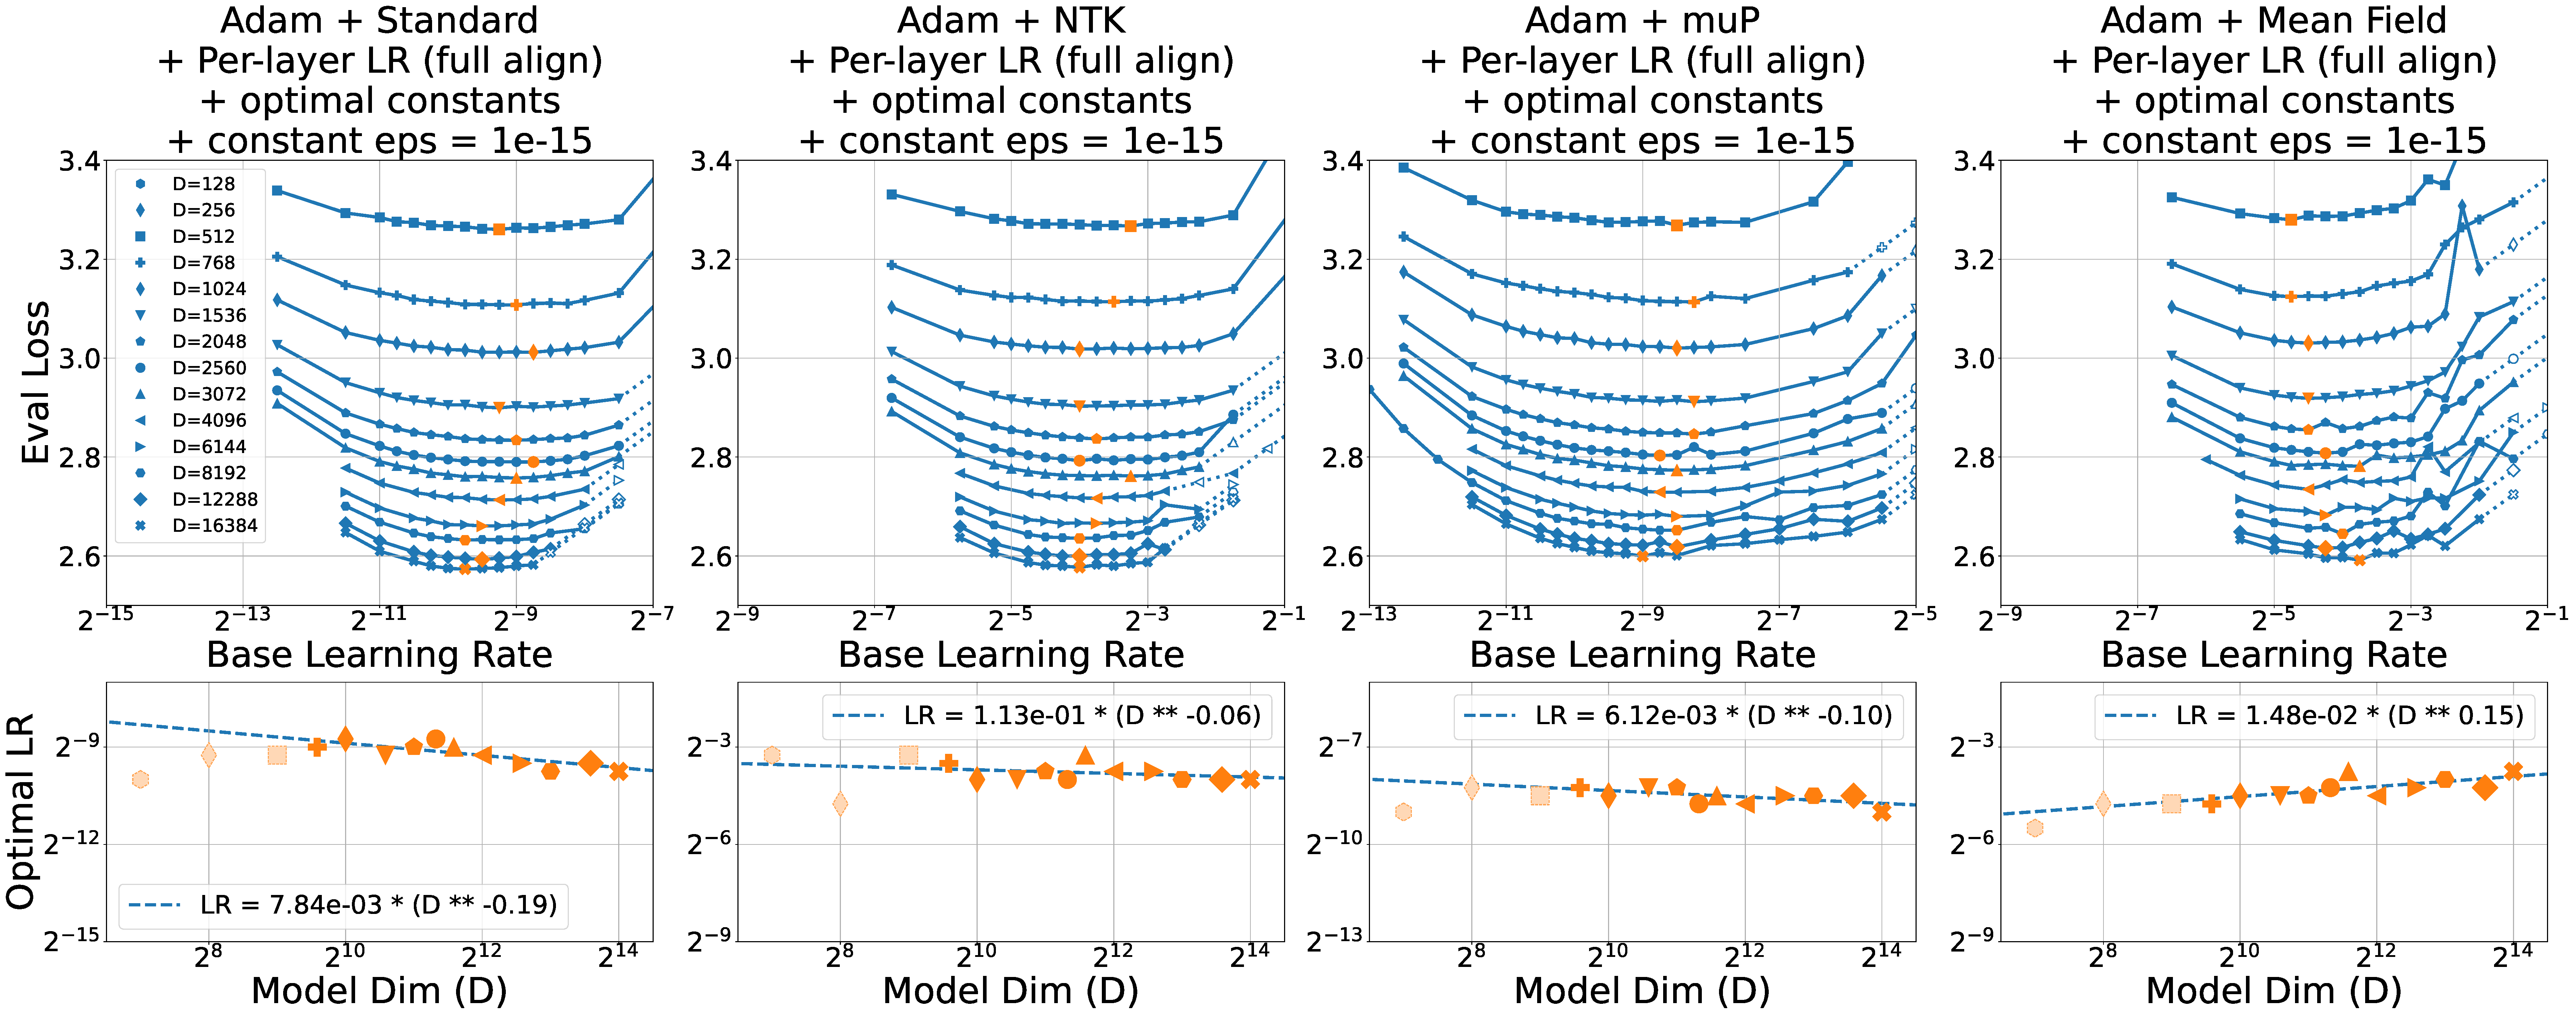
\includegraphics[width=\linewidth]{icml2024/figures/lr_sweeps/appendix/adam/adam+50k_steps_per_module_lr_optimal_constants_eps15.pdf}
\caption{Learning rate sweeps and power laws fit to optimal learning rate vs model dim. Top = Adam + per-layer learning rates assuming no alignment + optimal constants + per-layer epsilon with base epsilon = 1e-12. Bottom = Adam + per-layer learning rates assuming full alignment + optimal constants + constant epsilon = 1e-15. Number of training steps = $50{,}000$.}
\end{SidewaysFigure}
\clearpage

\thispagestyle{plain}
\begin{SidewaysFigure}
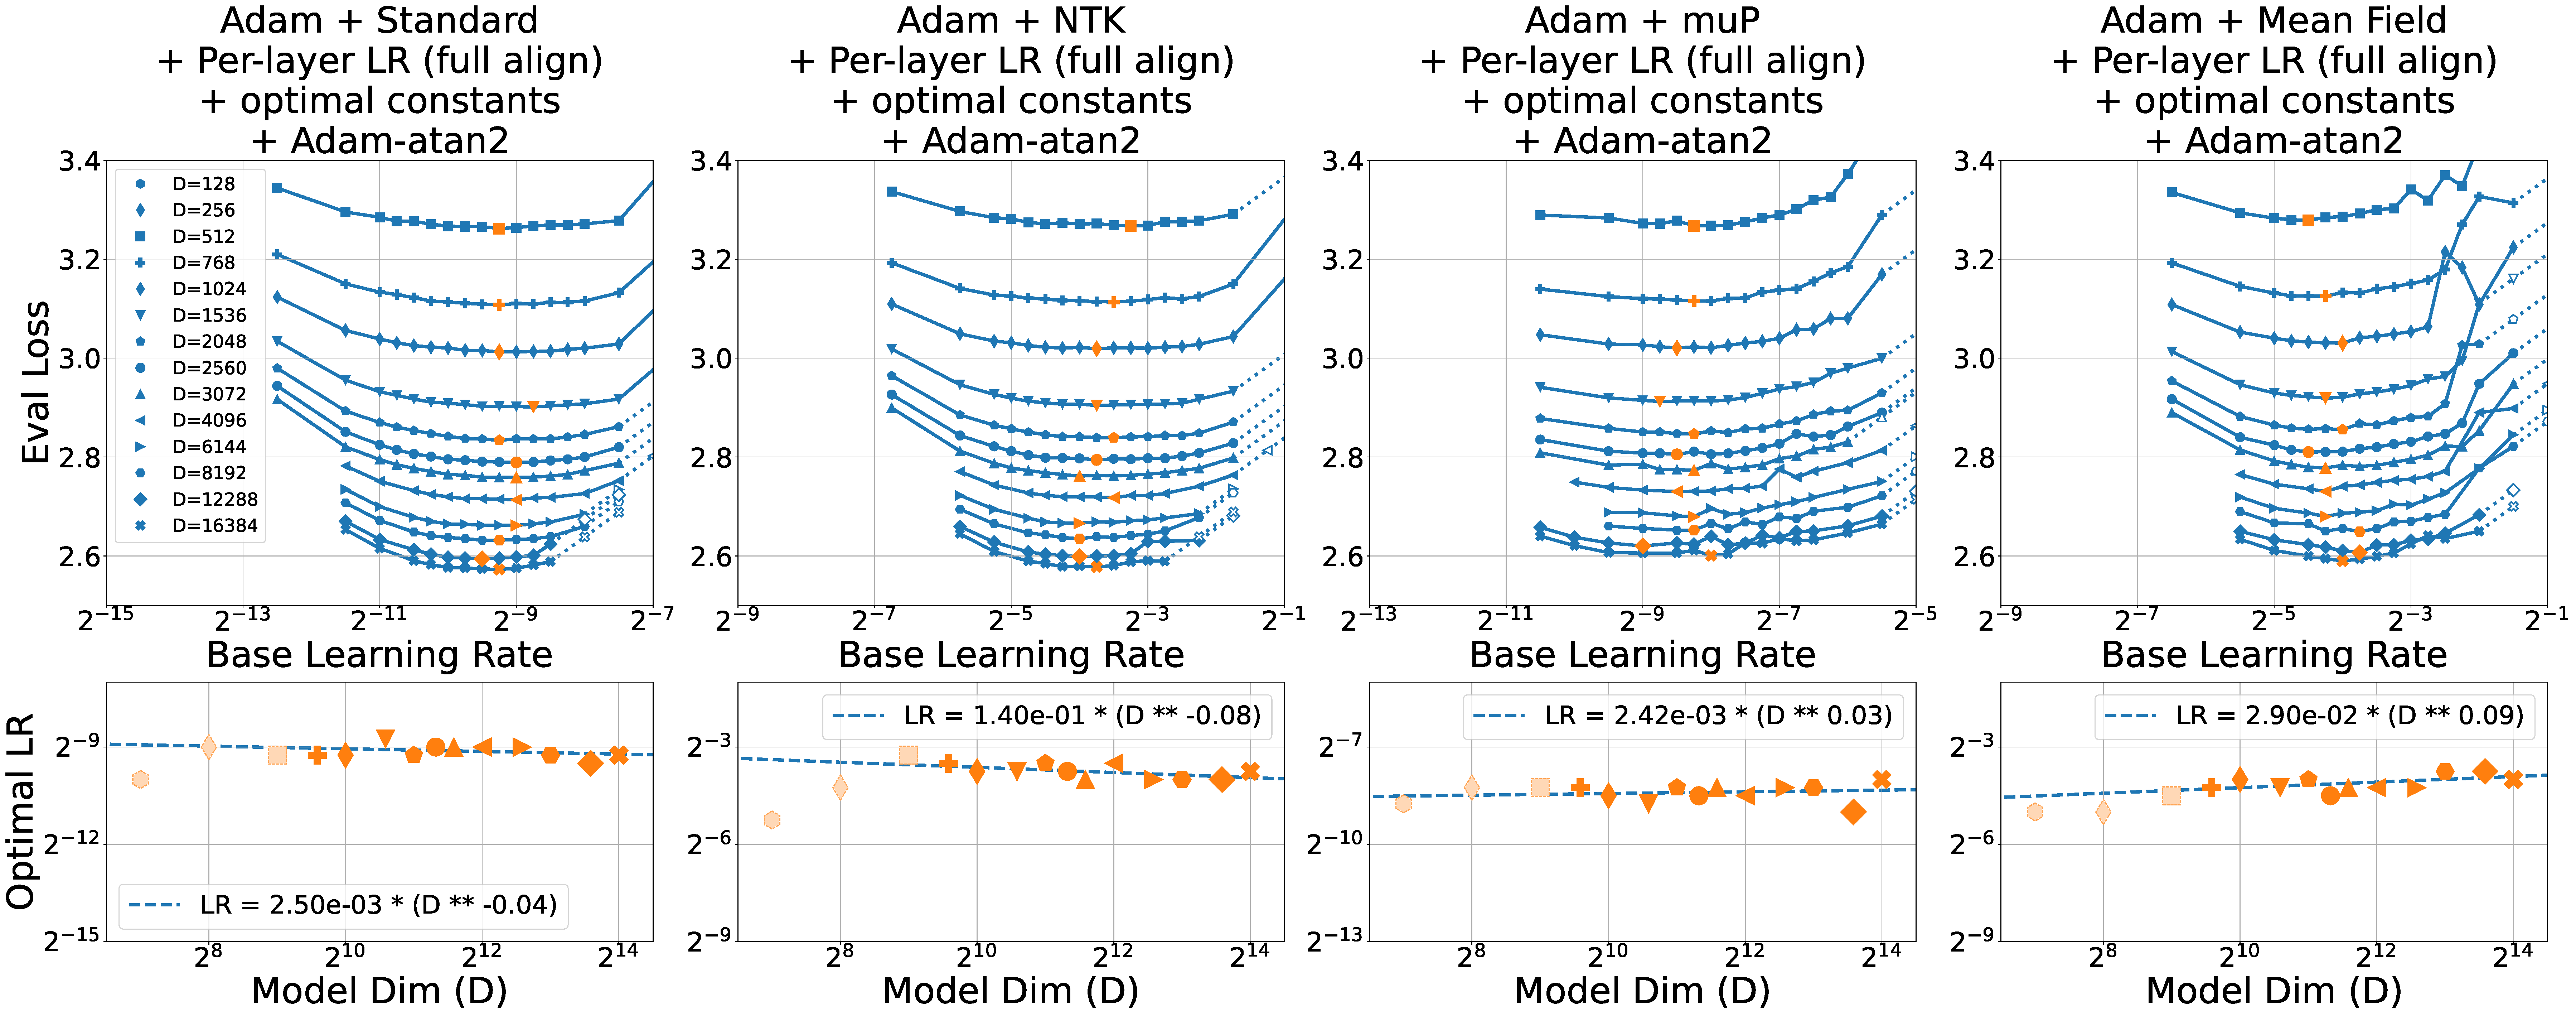
\includegraphics[width=\linewidth]{icml2024/figures/lr_sweeps/appendix/adam/adam+50k_steps_per_module_lr_optimal_constants_atan2_scale1.pdf}
\caption{Learning rate sweeps and power laws fit to optimal learning rate vs model dim. Adam-atan2 + per-layer learning rates assuming full alignment + optimal constants. Number of training steps = $50{,}000$.}
\end{SidewaysFigure}
\clearpage

\thispagestyle{plain}
\begin{SidewaysFigure}
\subsection{Learning Rate Sweeps for Adam + Parameter Scaling, all settings}
\label{sec:app_lr_sweeps_adam_ps}
\vspace{12pt}
\includegraphics[width=0.98\linewidth]{icml2024/figures/lr_sweeps/appendix/adam_ps/adam_ps+50k_steps_per_module_lr.pdf}

\figvspace

\includegraphics[width=0.98\linewidth]{icml2024/figures/lr_sweeps/appendix/adam_ps/adam_ps+50k_steps_per_module_lr_optimal_constants.pdf}
\caption{Learning rate sweeps and power laws fit to optimal learning rate vs model dim. Top = Adam + parameter scaling + per-layer learning rates assuming full alignment + default constants. Bottom = Adam + parameter scaling + per-layer learning rates assuming full alignment + optimal constants. Number of training steps = $50{,}000$.}
\label{fig:lr_sweep_adam_ps_full_align}
\end{SidewaysFigure}
\clearpage

\thispagestyle{plain}
\begin{SidewaysFigure}
\includegraphics[width=0.98\linewidth]{icml2024/figures/lr_sweeps/appendix/adam_ps/adam_ps+50k_steps.pdf}

\figvspace

\includegraphics[width=0.98\linewidth]{icml2024/figures/lr_sweeps/appendix/adam_ps/adam_ps+50k_steps_optimal_constants_only.pdf}
\caption{Learning rate sweeps and power laws fit to optimal learning rate vs model dim. Top = Adam + parameter scaling + per-layer learning rates assuming no alignment (equivalent to global learning rate) + default constants. Bottom = Adam + parameter scaling + per-layer learning rates assuming no alignment (equivalent to global learning rate) + optimal constants. Number of training steps = $50{,}000$.}
\label{fig:lr_sweep_adam_ps_no_align}
\end{SidewaysFigure}
\clearpage

\thispagestyle{plain}
\begin{SidewaysFigure}
\includegraphics[width=0.98\linewidth]{icml2024/figures/lr_sweeps/appendix/adam_ps/adam_ps+50k_steps_per_module_lr_optimal_constants_per_module_eps_base_eps12.pdf}

\figvspace

\includegraphics[width=0.98\linewidth]{icml2024/figures/lr_sweeps/appendix/adam_ps/adam_ps+50k_steps_per_module_lr_no_align_optimal_constants_per_module_eps_base_eps12.pdf}
\caption{Learning rate sweeps and power laws fit to optimal learning rate vs model dim. Top = Adam + parameter scaling + per-layer learning rates assuming full alignment + optimal constants + per-layer epsilon with base epsilon = 1e-12. Bottom = Adam + parameter scaling + per-layer learning rates assuming no alignment (equivalent to global learning rate) + optimal constants + per-layer epsilon with base epsilon = 1e-12. Number of training steps = $50{,}000$.}
\end{SidewaysFigure}
\clearpage


